\documentclass{article}
\title{The Ant Colony Optimisation for the Travelling Salesman Problem}
\author{Dylan Galea}
%Note since you added a sub section you will need to update some parts referring to a seciton.  IDEALLY LABEL SECTIONS

\usepackage{cite}
\usepackage{graphicx}
\usepackage{listings}
\usepackage[tbtags]{amsmath}
\usepackage{amsthm}
\usepackage{amssymb}
\usepackage{physics}
\usepackage{tikz}
\usepackage{pgfplots}
\usepackage{slashbox}
\usepackage{algpseudocode,algorithm,algorithmicx}
\usetikzlibrary{arrows.meta,automata,positioning}

\newtheorem{definition}{Definition}[subsection]
\newtheorem{theorem}[definition]{Theorem}
\newtheorem{lemma}[definition]{Lemma}
\newtheorem{corollary}[definition]{Corollary}
\newtheorem*{remark}{Remark}
\newtheorem{example}[definition]{Example}
\newtheorem{case}{Case}
\newtheorem{claim}{Claim}
\DeclareMathOperator*{\argmax}{argmax}

\begin{document}
\maketitle
\newpage
\tableofcontents
\newpage
\section{Introduction}
Before defining the Travelling Salesman Problem and proving properties about it, a number of graph theoretic concepts that will be used throughout, must first be defined. Therefore, what follows is a sub-section that introduces a number of graph theoretic concepts which are required for the Travelling Salesman Problem.
\subsection{Some Graph Theory}
Graph theory is the study of a structure called a graph. A graph can be defined formally as shown in definition \ref{Graph} below.
\begin{definition}
\label{Graph}
A graph G is a pair (V,E) were V is any non empty finite set called the set of vertices of G, and E $\subseteq$ \{$\{u,v\}$ $:$ $\forall$ u,v $\in$ V and u $\neq$ v\} is called the set of edges of G {\normalfont{\cite{black_tanenbaum_2017}}}. A graph G defined by the pair (V,E) is denoted by G(V,E) or G.
\end{definition}
A graph defined using definition \ref{Graph} is called an undirected graph. There is also the concept of a directed graph were $\mathit{E \subseteq \{(u,v) : \forall u,v \in V, u \neq v\}}$ \cite{black_tanenbaum_2017}. However, in this thesis it can be assumed that any graph that will be considered is undirected unless otherwise stated. It can also be assumed that there are no edges between same vertices unless otherwise stated. It must also be noted that by this definition, there cannot be multiple edges joining any 2 vertices. The reason is that sets do not allow repetition of elements. Thus, each element in the edge set is unique. The discussion will now proceed by introducing more graph theoretic terminology, with examples that illustrate these terminologies.\\
\\When two vertices are joined by an edge, they are said to be adjacent. This is defined formally in definition \ref{adjacent} below.
\begin{definition}
\label{adjacent}
Given a graph G(V,E), $\forall$ u,v $\in$ V, u and v are said to be adjacent if \{$u,v\}$ $\in$ E. Also, if u and v are adjacent, then u and v are said to be end vertices of the edge \{$u,v\}$. \normalfont{\cite{harris_hirst_mossinghoff_2008}}
\end{definition}
There is also a special name associated with the case when a vertex is an end vertex of an edge.
\begin{definition}
\label{incident}
A vertex v in a graph G is incident to an edge e in G if v is an end vertex of e. {\normalfont{\cite{harris_hirst_mossinghoff_2008}}}
\end{definition}
It is sometimes also required to know how many edges are incident to a specific vertex in a graph.
\begin{definition}
\label{degree}
The degree of a vertex v in a graph G denoted by deg(v) is, the number of edges incident with v in G. {\normalfont{\cite{harris_hirst_mossinghoff_2008}}}
\end{definition}
Any graph $\mathit{G(V,E)}$ can also be represented pictorially by drawing the vertices of $\mathit{G}$ using circles, and by drawing the edges of $\mathit{G}$ using lines between adjacent vertices. As a result, in this thesis a graph is sometimes given formally using sets or as a pictorial representation, assuming that one can be converted into another. Example \ref{Example 1} below depicts how a graph can be represented pictorially.
\begin{example}
\label{Example 1}
{\normalfont{Consider the graph}} G(V,E) {\normalfont{such that}}  V=\{$v_1, v_2, v_3, v_4\}$ {\normalfont{and}} E = \{$\{v_1, v_2\}, \{v_2,v_3\}, \{v_3,v_4\}, \{v_4,v_1\}\}$.\\{\normalfont{Then}} G {\normalfont{can be represented pictorially as :}}\\

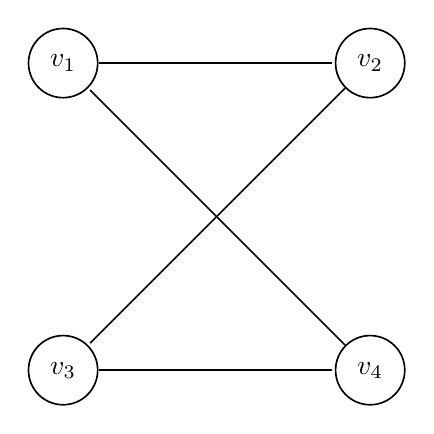
\begin{tikzpicture}[
    > = , % arrow head style
    shorten > = 1pt, % don't touch arrow head to node
    auto,
    node distance = 3cm, % distance between nodes
    semithick % line style
    ]

    \tikzset{every state}=[
    draw = black,
    thick,
    fill = black,
    minimum size = 1mm
    ]

    \node[state] (v1) {$v_1$};
    \node[state] (v2) [right=of v1] {$v_2$};
    \node[state] (v3) [below =of v1] {$v_3$};
    \node[state] (v4) [below =of v2] {$v_4$};
  
    \path[->] (v1) edge  node[]{}(v2);
    \path[->] (v2) edge  node[]{} (v3);
    \path[->] (v3) edge  node[]{}(v4);
    \path[->] (v4) edge  node[]{}(v1);
\end{tikzpicture}\\
{\normalfont{Using definition \ref{adjacent}, two adjacent vertices in }}G {\normalfont{are}} $v_1$ {\normalfont{and}} $v_2$.{\normalfont{ On the other hand, two non adjacent vertices in }}G {\normalfont{are}} $v_1$ {\normalfont{and}} $v_3.$\\ {\normalfont{By definition \ref{incident}}}, $v_1$ {\normalfont{and}} $v_2$ {\normalfont{are incident to the edge}} \{$v_1, v_2\}$.\\
{\normalfont{Using definition \ref{degree}, the degree of every vertex in}} G {\normalfont{is 2}}.
\end{example}
There are many other examples of graphs, one of them being the complete graph on $\mathit{n}$ vertices.
\begin{definition}
\label{Complete Graph}
A graph G(V,E) is said to be complete if $\forall$ v,w $\in$ V v $\neq$ w, v is adjacent to w. The complete graph on n vertices is denoted by $K_n$. \normalfont{\cite{harris_hirst_mossinghoff_2008}}
\end{definition}
Given any graph $\mathit{G(V,E)}$, one can also define graph theoretic structures that lie within $\mathit{G}$ such as walks and paths.
\begin{definition}
\label{walk}
Given a graph G(V,E), a walk is a sequence of vertices (not necessarily distinct) u= $u_1$, $u_2$, ...,$u_n$ = v such that, $\forall$ i $\in$ [n-1], $\{u_i, u_{i+1}\}$ $\in$ E. Such a walk is usually referred to as a u-v walk, were u and v are the end vertices of the walk. \normalfont{\cite{harris_hirst_mossinghoff_2008}}
\end{definition}
\begin{definition}
\label{Path}
Given a graph G(V,E), a path in G joining any 2 vertices u, v $\in$ V, is a u-v walk with no repeated vertices.
\end{definition}
Definition \ref{Path} can now be used to define cycles and connectivity in a graph.
\begin{definition}
\label{connectedgraph}
A graph G(V,E) is said to be connected if $\forall$ u,v $\in$ V u $\neq$ v, u and v are joined by a path. \normalfont{\cite{harris_hirst_mossinghoff_2008}}
\end{definition}
\begin{definition}
\label{cycle}
Given a graph G(V,E), a cycle in G is a path on n $\geq$ 4 vertices, such that, the first vertex and the last vertex are equal. \normalfont{\cite{cycle}} 
\end{definition}
By Definitions \ref{walk}, \ref{Path} above, it is clear that a path is a special instance of a walk. Similarly from Definitions \ref{Path} and \ref{cycle}, a cycle is a special instance of a path, with the only difference being that in a cycle, the first vertex and the last vertex are equal. Another thing worth mentioning is that, according to definitions \ref{walk}, \ref{Path} and \ref{cycle}, since cycles and paths are formulated in terms of walks, then they are sequences of vertices and not actual graphs. However, this is not the case because they can be represented easily as graphs. For example, given the path/cycle $\mathit{u_1, u_2, ...,u_n}$ a new graph $\mathit{G(V,E)}$ can be created such that, $\mathit{V= \{ u_1, u_2, ..., u_n\}}$ and $\mathit{E = \{ \{u_i, u_{i+1}\} : \forall i, 0 < i < n\}}$. For example, consider the cycle $v_1$, $v_2$, $v_3$, $v_4$, $v_1$, then the graph depicted in example \ref{Example 1}, is the graph representing this cycle. Such graphs are known as Cycle/Path graphs and are denoted by $\mathit{C_n/P_n}$ respecitvely, $\mathit{n}$ being the number of vertices in the graph. Since this construction can be done, cycles/paths will be treated as both graphs and sequences throughout this project. This will later be useful when defining Hamiltonian cycles. For better understanding of definitions \ref{Complete Graph}, \ref{Path}, \ref{connectedgraph} and \ref{cycle}, example \ref{example3} is constructed.
\begin{example}
\label{example3}
{\normalfont{Consider the graph}} G(V,E) {\normalfont{below:}}\\
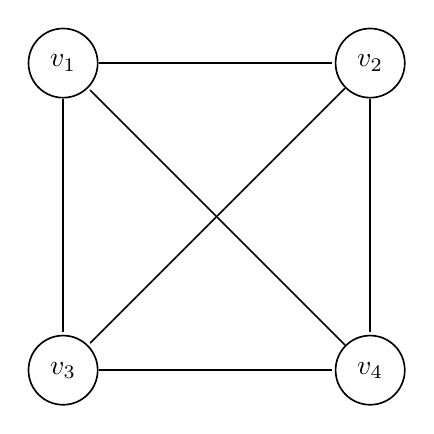
\begin{tikzpicture}[
    > = , % arrow head style
    shorten > = 1pt, % don't touch arrow head to node
    auto,
    node distance = 3cm, % distance between nodes
    semithick % line style
    ]

    \tikzset{every state}=[
    draw = black,
    thick,
    fill = black,
    minimum size = 1mm
    ]

    \node[state] (v1) {$v_1$};
    \node[state] (v2) [right=of v1] {$v_2$};
    \node[state] (v3) [below =of v1] {$v_3$};
    \node[state] (v4) [below =of v2] {$v_4$};
  
    \path[->] (v1) edge  node[]{}(v2);
    \path[->] (v1) edge  node[]{}(v3);
    \path[->] (v2) edge  node[]{} (v3);
    \path[->] (v3) edge  node[]{}(v4);
    \path[->] (v2) edge  node[]{}(v4);
    \path[->] (v4) edge  node[]{}(v1);
\end{tikzpicture}
\\
{\normalfont{Since every vertex in}} G {\normalfont{is adjacent to every other vertex, }}G {\normalfont{must be complete. Therefore}} G {\normalfont{must be}} $K_4$. {\normalfont{Since}} G {\normalfont{is complete, it must also be connected because, there is a path}} $P_2$ {\normalfont{between any two distinct vertices of}} G.\\
{\normalfont{Some examples of walks in}} G {\normalfont{are:}}\\
1. $v_1$ $v_2$ $v_3$ $v_4$ $v_1$ $v_2$\\
2. $v_1$ $v_4$ $v_2$ $v_3$ $v_1$ $v_3$\\
3. $v_4$ $v_3$ $v_1$ $v_4$ $v_1$\\
{\normalfont{Some examples of paths in}} G {\normalfont{are:}}\\
1. $v_1$ $v_2$ $v_3$ $v_4$\\
2. $v_1$ $v_4$\\
3. $v_4$ $v_3$ $v_1$\\
{\normalfont{Some examples of cycles in}} G {\normalfont{are:}}\\
1. $v_1$ $v_2$ $v_3$ $v_4$ $v_1$\\
2. $v_1$ $v_4$ $v_2$ $v_3$ $v_1$\\
3. $v_4$ $v_3$ $v_1$ $v_4$
\end{example}
 Another important graph theoretic concept is that of subgraphs. 
\begin{definition}
\label{subgraph}
Given a graph G(V,E) and a graph H($V^\prime$,$E^\prime$), H is a subgraph of G if $V^\prime$ $\subseteq$ V and $E^\prime$ $\subseteq$ E.  \normalfont{\cite{harris_hirst_mossinghoff_2008}}
\end{definition}
Clearly by definition \ref{subgraph} and the construction of Cycle/Path graphs, if $A$ is a cycle/path in $G$ then the Cycle/Path graph representing $A$ is a subgraph of $G$. This leads to defining the concept of two distinct path/cycles. Two paths/cycles in $G$ are said to be distinct if, when they they are constructed as Path/Cycle subgraphs of $G$ they differ in at least one edge. After defining some important concepts, the next step is to extend definition \ref{Graph} to define another class of graphs called weighted graphs. It must be noted that all definitions presented so far apply also to weighted graphs.
\begin{definition}
\label{Weighted Function}
Given a graph G(V,E), a weight function is a function f : E $\mapsto$ $\real^+$ {\normalfont{\cite{harris_hirst_mossinghoff_2008}}}. The real numbers assigned to each edge are called weights.
\end{definition}
Note that in definition \ref{Weighted Function}, the weights are taken to be positive. According to \cite{harris_hirst_mossinghoff_2008}, there could be cases were negative weights would be appropiate. However, unless otherwise stated, it is to be assumed that when considering a weight function, the weights are positive.
\begin{definition}
\label{Weighted Graph}
A weighted graph is a graph G(V,E) with a weight function f {\normalfont{\cite{harris_hirst_mossinghoff_2008}}}. This is denoted by the triple G(V,E,f) or G. 
\end{definition}
According to Bondy and Murty \cite{bondy_murty_1982}, weighted graphs occur regularly in applied graph theory. For example, a railway network can be represented by a weighted graph were, the vertices are the set of towns in the railway network, and there are edges between 2 vertices in the graph if, there is a direct route from one town to another, without visiting other towns in the process. The weight function would then represent the cost of travelling directly from one town to another. In addition to that, the shortest path between 2 towns in the network may be required. It is clear that in order to try and solve such problems, the total weight of a subgraph must first be defined.
\begin{definition}
\label{weightofasubgraph}
Given a weighted graph G(V,E,f), the total weight of any subgraph  H($V^\prime$,$E^\prime$,f) of G is: $$\sum_{e \in E^\prime}^{} f(e) $$. \normalfont{\cite{bondy_murty_1982}}
\end{definition}
It is important to note that by definition \ref{subgraph}, any weighted graph G is a subgraph of itself, therefore, it's weight can be calculated. This is highlighted in Example \ref{example4} below.
\begin{example}
\label{example4}
{\normalfont{Consider the weighted graph}} G(V,E,f) {\normalfont{such that,}} G(V,E) {\normalfont{ is the graph in example \ref{example3} with weight function}} f {\normalfont{such that}},\\
f(\{$v_1, v_2\}$) = 4\\
f(\{$v_1, v_3\}$) = 5\\
f(\{$v_2, v_3\}$) = 2\\
f(\{$v_3, v_4\}$) = 10\\
f(\{$v_2, v_4\}$) = 4\\
f(\{$v_4, v_1\}$) = 7\\
{\normalfont{Then by definition \ref{Weighted Graph}, the graph below is a weighted graph}}.\\
\end{example}
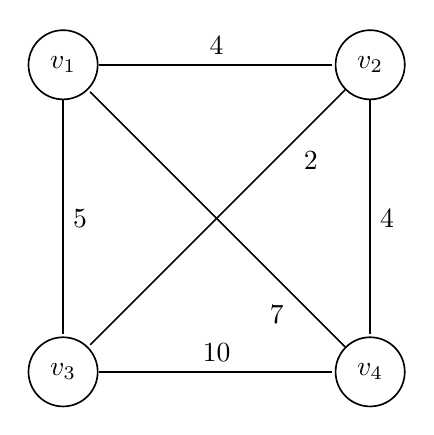
\begin{tikzpicture}[
    > = , % arrow head style
    shorten > = 1pt, % don't touch arrow head to node
    auto,
    node distance = 3cm, % distance between nodes
    semithick % line style
    ]

    \tikzset{every state}=[
    draw = black,
    thick,
    fill = white,
    minimum size = 1mm
    ]
    \node[state] (v1) {$v_1$};
    \node[state] (v2) [right=of v1] {$v_2$};
    \node[state] (v3) [below =of v1] {$v_3$};
    \node[state] (v4) [below =of v2] {$v_4$};
  
    \path[->] (v1) edge  node[]{4}(v2);
    \path[->] (v1) edge  node[]{5}(v3);
    \path[->] (v2) edge  node[pos=0.2,below right]{2} (v3);
    \path[->] (v3) edge  node[]{10}(v4);
    \path[->] (v2) edge  node[]{4}(v4);
    \path[->] (v4) edge  node[pos=0.2,below left]{7}(v1);
\end{tikzpicture}\\
 {\normalfont{Also according to definition \ref{subgraph}, the above graph is a subgraph of itself. Therefore it's weight can be calculated, where by definition \ref{weightofasubgraph}, the weight of}} G {\normalfont{is 32.}}\\
\\
According to Guichard \cite{guichard_2018}, trees are another useful class of graphs.
\begin{definition}
\label{tree}
A tree is a connected graph with no cycles. \normalfont{\cite{guichard_2018}}
\end{definition}
Having defined the basic graph theoretic concepts, it is now time to define harder concepts that use previous definitions. It is important to note that the following concepts can be applied to both weighted and unweighted graphs. Therefore, in the remaining definitions the graph being considered can either be weighted or unweighted.
\begin{definition}
\label{spanning subgraph}
H($V^\prime$,$E^\prime$) is a spanning subgraph of G(V,E) if H is a subgraph of G and $V^\prime$ = V. \normalfont{\cite{ray_2013}}
\end{definition}
There are many spanning subgraphs, however the ones that are relevant to this thesis are spanning trees and spanning cycles, the latter mostly known as Hamiltonian cycles.
\begin{definition}
A graph H is a spanning tree of G if H is a tree and H is a spanning subgraph of G. \normalfont{\cite{ray_2013}}
\label{spanning tree}
\end{definition}
\begin{definition}
\label{hamiltonian cycle}
Given a graph G, C is a Hamiltonian cycle in G if C is a cycle and C is a spanning subgraph of G. Also, a graph that contains a Hamiltonian cycle is called a Hamiltonian graph. \normalfont{\cite{ray_2013}}
\end{definition}
It is worth mentioning that definition \ref{hamiltonian cycle} holds because, cycles can be represented by Cycle graphs due to the construction discussed earlier. What follows now is an example that illustrates better definitions \ref{spanning subgraph}, \ref{spanning tree} and \ref{hamiltonian cycle}. 
\begin{example}
\label{example5}
{\normalfont{Let}} G {\normalfont{be the graph in example \ref{example4}. Then, according to definition \ref{spanning subgraph}, the two graphs below are two spanning subgraphs of}} G {\normalfont{because, they contain all the vertices of}} G {\normalfont{and are subgraphs of }}G .\\
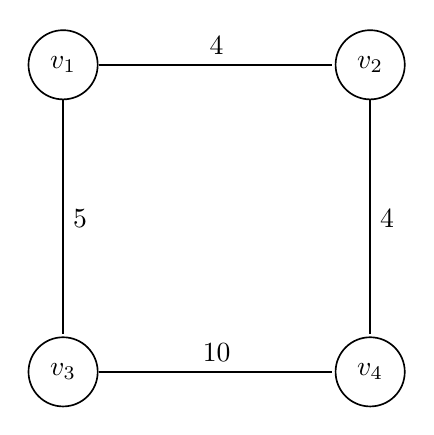
\begin{tikzpicture}[
    > = , % arrow head style
    shorten > = 1pt, % don't touch arrow head to node
    auto,
    node distance = 3cm, % distance between nodes
    semithick % line style
    ]

    \tikzset{every state}=[
    draw = black,
    thick,
    fill = white,
    minimum size = 1mm
    ]
    \node[state] (v1) {$v_1$};
    \node[state] (v2) [right=of v1] {$v_2$};
    \node[state] (v3) [below =of v1] {$v_3$};
    \node[state] (v4) [below =of v2] {$v_4$};
  
    \path[->] (v1) edge  node[]{4}(v2);
    \path[->] (v1) edge  node[]{5}(v3);
    \path[->] (v3) edge  node[]{10}(v4);
    \path[->] (v2) edge  node[]{4}(v4);
\end{tikzpicture}\\
\\
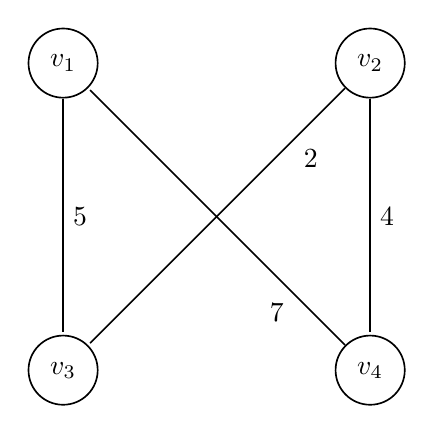
\begin{tikzpicture}[
    > = , % arrow head style
    shorten > = 1pt, % don't touch arrow head to node
    auto,
    node distance = 3cm, % distance between nodes
    semithick % line style
    ]

    \tikzset{every state}=[
    draw = black,
    thick,
    fill = white,
    minimum size = 1mm
    ]
    \node[state] (v1) {$v_1$};
    \node[state] (v2) [right=of v1] {$v_2$};
    \node[state] (v3) [below =of v1] {$v_3$};
    \node[state] (v4) [below =of v2] {$v_4$};
  
    \path[->] (v1) edge  node[]{5}(v3);
    \path[->] (v2) edge  node[pos=0.2,below right]{2} (v3);
    \path[->] (v2) edge  node[]{4}(v4);
    \path[->] (v4) edge  node[pos=0.2,below left]{7}(v1);
\end{tikzpicture}\\
{\normalfont{It must also be said that by definition \ref{hamiltonian cycle}, the above two graphs are Hamiltonian cycles in}} G {\normalfont{because, they are spanning sub-graphs of}} G {\normalfont{and are Cycle sub-graphs of}} G. {\normalfont{Since the above graphs are sub-graphs of }}G{\normalfont{, by definition \ref{weightofasubgraph}, their weight can be calculated by summing up the weights of the edges. Thus, the Hamiltonian cycles above have weight 23 and 18 respectively.}}\\
{\normalfont{Given the same graph }}G{\normalfont{ in example \ref{example4}, the two graphs below are spanning trees of }}G{\normalfont{ of weight 18 and 19 respectively.}}\\
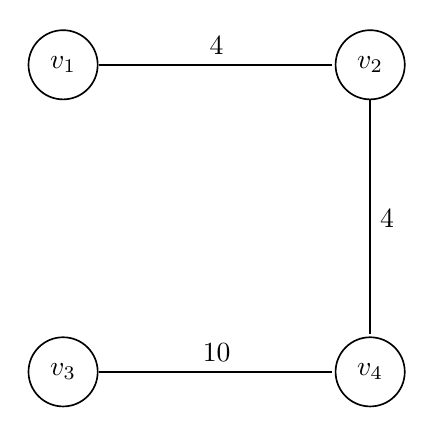
\begin{tikzpicture}[
    > = , % arrow head style
    shorten > = 1pt, % don't touch arrow head to node
    auto,
    node distance = 3cm, % distance between nodes
    semithick % line style
    ]

    \tikzset{every state}=[
    draw = black,
    thick,
    fill = white,
    minimum size = 1mm
    ]
    \node[state] (v1) {$v_1$};
    \node[state] (v2) [right=of v1] {$v_2$};
    \node[state] (v3) [below =of v1] {$v_3$};
    \node[state] (v4) [below =of v2] {$v_4$};
  
    \path[->] (v1) edge  node[]{4}(v2);
    \path[->] (v3) edge  node[]{10}(v4);
    \path[->] (v2) edge  node[]{4}(v4);
\end{tikzpicture}\\
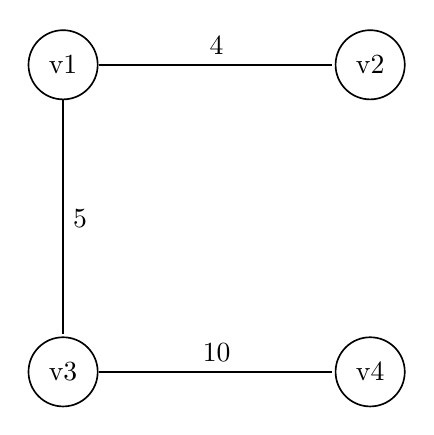
\begin{tikzpicture}[
    > = , % arrow head style
    shorten > = 1pt, % don't touch arrow head to node
    auto,
    node distance = 3cm, % distance between nodes
    semithick % line style
    ]

    \tikzset{every state}=[
    draw = black,
    thick,
    fill = white,
    minimum size = 1mm
    ]
    \node[state] (v1) {v1};
    \node[state] (v2) [right=of v1] {v2};
    \node[state] (v3) [below =of v1] {v3};
    \node[state] (v4) [below =of v2] {v4};
  
    \path[->] (v1) edge  node[]{4}(v2);
    \path[->] (v1) edge  node[]{5}(v3);
    \path[->] (v3) edge  node[]{10}(v4);
\end{tikzpicture}\\
{\normalfont{This example also shows that within the same weighted graph, there could be multiple Hamiltonian cycles and spanning trees of different weight.}}
\end{example}
Having defined Hamiltonian cycles and spanning trees, it is natural to ask whether there are necessary and sufficient conditions in a graph that guarantee it is Hamiltonian or that it contains a spanning tree as sub-graph. In fact, theorem \ref{spanningtreetheorem} gives a necessary and sufficient condition for a graph to have a spanning tree.
\begin{theorem}
A graph G has a spanning tree $\iff$ it is connected {\normalfont{\cite{ray_2013}}}.
\label{spanningtreetheorem}
\end{theorem} 
\begin{proof}
($\implies$) Let $\mathit{G(V,E)}$ be a graph having a spanning tree $\mathit{T(V^\prime,E^\prime)}$ as one of it's subgraphs. Let $\mathit{v1, v2}$ $\in$ $\mathit{V}$. Since, $\mathit{T}$ is a spanning tree of $\mathit{G}$, then, $\mathit{T}$ is a spanning subgraph of $\mathit{G}$. Thus, $\mathit{v1, v2}$ $\in$ $V^\prime$. Also, since $\mathit{T}$ is a tree, $\mathit{T}$ must be connected. Therefore, $\exists$ a path $\mathit{P}$ joining vertices $\mathit{v_1}$ and $\mathit{v_2}$ in $\mathit{T}$. But since $\mathit{T}$ is a subgraph of G, then $\mathit{P}$ is also a path in $\mathit{G}$. Therefore $\mathit{G}$ must be connected.\\
($\Leftarrow$) Conversely, let $\mathit{G(V,E)}$ be a connected graph. Then, if $\mathit{G}$ has no cycles, $\mathit{G}$ itself must be a spanning tree. If $\mathit{G}$ has cycles, delete an edge from a cycle in $\mathit{G}$. Clearly, the resultant graph is still connected and contains one less cycle. Repeat this procedure untill no more cycles are left in the graph. Then, the resultant graph $\mathit{G^\prime}$ would be a connected subgraph of $\mathit{G}$ having no cycles(i.e a tree). Also, since by the deletion procedure, no vertex was deleted from $\mathit{G}$, $\mathit{G^\prime}$ is a spanning subgraph of $\mathit{G}$. Therefore $\mathit{G^\prime}$ is a spanning tree of $\mathit{G}$. \normalfont{\cite{ray_2013}}
\end{proof}
Theorem \ref{spanningtreetheorem} confirms that for a graph to have a spanning tree, the graph must be connected and vice-versa. Thus, for spanning trees, the necessary and sufficient condition is connectivity. However, the same cannot be said about Hamiltonian cycles because, no necessary and sufficient conditions are known for a graph to be Hamiltonian. In fact, there are sufficient conditions for a graph to be Hamiltonian, however, these conditions are not necessary. There are also necessary conditions, some of which are trivial, such as, if $\mathit{G}$ is Hamiltonian then G must be connected, but this is not necessary and sufficient. According to Guichard \cite{guichard_2018}, these sufficient conditions typically say that for a graph to be Hamiltonian it must have a lot of edges. But it is also argued in \cite{guichard_2018}, that these conditions are not necessary, because, there are Hamiltonian graphs that have few edges. For example, $\mathit{C_n}$ has only $\mathit{n}$ edges but is Hamiltonian. One such sufficient but not necessary condition for Hamiltonianicity is Ore's Theorem below.
\begin{theorem}[Ore's Theorem]
\label{ore's theorem}
Let G be a graph on n $\geq$ 3 vertices such that if v and w are not adjacent in G then deg(v) + deg(w) $\geq$ n. Then G is Hamiltonian. {\normalfont{\cite{ray_2013}}}
\end{theorem}
\begin{proof}
Suppose that $\mathit{G(V,E)}$ is a graph satisfying all the conditions in the theorem statement but is not Hamiltonian. Then since $\mathit{G}$ is not Hamiltonian and $K_n$ is Hamiltonian, $\mathit{G}$ must be a subgraph of $\mathit{K_n}$ having fewer edges than $\mathit{K_n}$. Therefore, add edges to $\mathit{G}$ between non adjacent vertices to obtain a subgraph $\mathit{H(V^\prime,E^\prime)}$ of $\mathit{K_n}$ such that adding an edge to $\mathit{H}$ would create a subgraph of $\mathit{K_n}$ which is Hamiltonian. Let $\mathit{u, v}$ $\in$ $V^\prime$ be 2 non-adjecent vertices in H. Since by construction $\mathit{G}$ is a subgraph of $\mathit{H}$, $\mathit{u, v}$ must be non-adjcent in $\mathit{G}$. Therefore $\mathit{deg(u) + deg(v) \geq n}$ in both G and H. Since adding an edge to $\mathit{H}$ creates a resultant graph that is Hamiltonian, then, adding an edge between $\mathit{u}$ and $\mathit{v}$ creates a Hamiltonian graph. Therefore, in $\mathit{H}$ there must be a path joining $\mathit{u}$ and $\mathit{v}$ containing all the vertices of $\mathit{H}$. Let the path be $\mathit{u = v_1, v_2, ..., v_n = v}$.\\
Now suppose $\mathit{deg(v_1)}$ = $\alpha$ in $\mathit{H}$. Now $\forall \mathit{i}, 1 <  i < \mathit{n}$, if there is an edge between $\mathit{u_1}$ and $\mathit{u_i}$ in $\mathit{H}$, then there must not be an edge between $\mathit{u_{i-1}}$ and $\mathit{u_n}$ because, $\mathit{u_1, u_i, u_{i+1}, ..., u_n, u_{i-1}, u_{i-2}, ..., u_1}$ would be a Hamiltonian cycle in $\mathit{H}$, thus H would be Hamiltonian. Therefore, $\mathit{deg(u_n)}$ $\leq$ $\mathit{n-1-\alpha}$\\
$\implies$ $\mathit{deg(u_1) + deg(u_n) \leq \alpha +  n-1 - \alpha}$ in $\mathit{H}$\\
$\implies$ $\mathit{deg(u_1) + deg(u_n) \leq n-1}$ in $\mathit{H}$\\
$\implies$ $\mathit{deg(u_1) + deg(u_n) < n}$ in $\mathit{G}$ since $\mathit{G}$ is a subgraph of $\mathit{H}$.\\
This contradicts the assumption that $\mathit{deg(u_1 = u) + deg(u_n = v) \geq n}$ in $\mathit{G}$ \\
Therefore, $\mathit{G}$ must be Hamiltonian. \cite{ray_2013}
\end{proof}
It is important to note that the above proof uses the fact that $K_n$ is Hamiltonian. This is true because any $C_n$ is always a subgraph of $K_n$. Therefore any $C_n$ that spans $K_n$ is a subgraph of $K_n$. Example \ref{example 6} below is a counter example to show why Ore's theorem gives a sufficient but not necessary condition.\\
\begin{example}
\label{example 6}
{\normalfont{Consider the graph}} $C_5$ below.
\\
\begin{tikzpicture}[
    > = , % arrow head style
    shorten > = 1pt, % don't touch arrow head to node
    auto,
    node distance = 3cm, % distance between nodes
    semithick % line style
    ]

    \tikzset{every state}=[
    draw = black,
    thick,
    fill = white,
    minimum size = 1mm
    ]
    \node[state] (v1) {$v_1$};
    \node[state] (v2) [below left =of v1] {$v_2$};
    \node[state] (v3) [below right =of v1] {$v_3$};
    \node[state] (v4) [below=of v2] {$v_4$};
    \node[state] (v5) [below=of v3] {$v_5$};

    \path[->] (v1) edge  node[]{}(v2);
    \path[->] (v2) edge  node[]{}(v4);
    \path[->] (v4) edge  node[]{}(v5);
    \path[->] (v5) edge  node[]{}(v3);
    \path[->] (v3) edge  node[]{}(v1);
\end{tikzpicture}\\
$C_5$ {\normalfont{above is Hamiltonian because it contains the Hamiltonian cycle}} $v_1, v_2, v_4, v_5, v_3, v_1$. {\normalfont{However,}} deg($v_1$) + deg($v_5$) = 4 $<$ 5 = n. {\normalfont{Therefore, the condition in Ore's Theorem is not a necessary condition}}.
\end{example} 
To conclude, these facts seem to indicate that determining whether a graph is Hamiltonian is a very difficult problem and that there are certain problems that are harder than other problems. In order to reason about such problems, some computational theory must first be established. This is done in the next subsection.
\subsection{Some Computational Theory}
After defining some important graph theoretic concepts, it is now time to present some important computational theory that will be used in later sections. The discussion will now proceed by defining two different types of problems and describing the relationship between them.
\begin{definition}
\label{optimization problems}
Suppose that a problem P has many possible solutions such that each solution has an associated value. Then P is an optimisation problem if P requires to find the solution with the best value.  \normalfont{\cite{cormen_leiserson_rivest_stein}}
\end{definition}
Therefore, according to definition \ref{optimization problems}, the aim of the algorithm solving an optimisation problem would then be to find the solution with the best (min/max) value. An maximisation problem is an optimization problem that asks to find the solution with the maximum value. On the other hand, a minimisation problem is an optimisation problem that asks to find the solution with the minimum value. The solution with the best value is called an optimal solution to the problem, and it's value is known as the optimal value. An optimal solution is not termed as `the' optimal solution because, there could be many optimal solutions having the same optimal value. \cite{cormen_leiserson_rivest_stein} \\\\Another type of problems is called decision problems.
\begin{definition}
\label{decision problems}
Decision problems are problems whose solutions are either a yes or a no. \normalfont{\cite{cormen_leiserson_rivest_stein}}
\end{definition}
In \cite{cormen_leiserson_rivest_stein} it is argued that, given an optimisation problem, one can transform this optimisation problem into a decision problem such that, the decision problem is easier than the optimisation problem. Therefore, if some optimisation problem is easy to solve, the decision problem version is easy to solve as well \cite{cormen_leiserson_rivest_stein}. On the other hand, if the decision problem is hard to solve then this would mean that the original optimization problem is also hard to solve \cite{cormen_leiserson_rivest_stein}. Note that the notion of `hard' and `easy' problems will be defined rigorously later in this section. This concept was only mentioned here to show that there exists a relationship between optimisation problems and decision problems. Before going into harder computational theory, an example is given to undestand how an optimisation problem can be transformed into a related decision problem.
\begin{example}
\label{example decision/optimization}
{\normalfont{Two optimisation problems are:\\
1. The shortest path problem\\
2. The minimum weight spanning tree problem\\
Given a connected weighted graph}} G{\normalfont{, the shortest path problem is the task of finding a path}} P {\normalfont{between two vertices in}} G {\normalfont{such that, the weight of }}P {\normalfont{is the minimum amongst all paths joining these two vertices in }}G {\normalfont{\cite{hackerearth_blog}}}. {\normalfont{On the other hand, given a  connected weighted graph}} G {\normalfont{the minimum weight spanning tree problem is the task of finding a spanning tree in}} G {\normalfont{of minimum weight \cite{geeksforgeeks}. The shortest path problem is an optimsation problem because, from all the possible paths in the graph, a path having the optimal value (minimum weight) is chosen. In this case the best path is the path with minimum weight. Similarly, using the same reasoning, the minimum weight spanning tree problem is an optimisation problem. }}\\
{\normalfont{The decision problems related to these optimisation problems can be obtained by specifying a bound on the value to be optimized \cite{cormen_leiserson_rivest_stein}. Therefore, the decision problems related to the shortest path problem, and the minimum weight spanning tree problem defined in this example are:}}\\
{\normalfont{1.Given a connected weighted graph}} G, {\normalfont{two vertices}} u {\normalfont{and}} v, {\normalfont{and an integer}} k,{\normalfont{ does a path exist from}} u {\normalfont{to}} v {\normalfont{in}} G {\normalfont{of weight at most}} k?\\
{\normalfont{2.Given a connected weighted graph}} G, {\normalfont{and an integer}} k{\normalfont{, does}} G {\normalfont{contain a spanning tree of weight at most}} k?\\
{\normalfont{The above two problems are decision problems because the answer to these problems is either a yes or a no.}}
\end{example}
Reasoning about computational problems is usually done by analyzing the properties belonging to the algorithms that solve these problems. One property that is analyzed is called the running time of an algorithm. This is defined in definition \ref{running_time} below.
\begin{definition}
\label{running_time}
Given an input I, the running time of an algorithm A is the number of steps executed by A given I. The running time of an algorithm A can be represented by the function T $:$ $\mathbb{N}$ $\mapsto$ $\mathbb{N}$ were the domain represents the size of the input, and the co-domain represents the amount of steps taken by the algorithm to execute given an input size. {\normalfont{\cite{cormen_leiserson_rivest_stein}, \cite{adamchik_2009}}}
\end{definition}
The following is an example on how the running time of an algorithm can be constructed.
\begin{example}
\label{example_running}
{\normalfont{Consider an algorithm that performs the addition of two}} n-{{\normalfont{bit strings. Then if the addition of 2 bits takes}}} a {\normalfont{computational steps, the addition of 2}} $\mathit{n-}${\normalfont{bit strings will take}} a $\times$ n {\normalfont{steps, since, each computation must be performed}} n {\normalfont{times (i.e on each bit in the string). Therefore, the running time of this algorithm for an input of size}} n {\normalfont{can be represented by the function,\\}} T(n) = a $\times$ n. {\normalfont{\cite{cormen_leiserson_rivest_stein}, \cite{adamchik_2009}}}
\end{example}
Expressing the running time in this way seems pretty easy to understand. However, it has problems. Typically, the running time of an algorithm is fixed for any input, however, the running time function is not defined on the actual inputs, but, on the input sizes. As a result, since the same input size might represent different inputs, there could be different running times for the same input size $\mathit{n}$, as this depends on which input is given. This means that for any input size $\mathit{n}$, there are different running time functions giving different running times. These different running time functions represent the different cases that could arise in an algorithm given any input size $\mathit{n}$. The most important runnning time functions are the worst-case running time, the best-case running time and the average-case running time. The worst/best/average case running time are the longest/shortest/average running time of an algorithm given any input of size $\mathit{n}$ respectively. Therefore the problem is what running time function should be used to reason about algorithms. Although the average-case running time generally has a greater practical significance, it is often very difficult to compute. Therefore, the worst-case running time is usually used, that is, finding the running time function that gives the worst-case running time for any input of size $\mathit{n}$. The worst-case running time of an algorithm is an upper bound to all other running times, therefore, this assures that the algorithm will never get a longer running time for any input of size $\mathit{n}$. So, if the worst case running time is polynomial in the input size, then we know that the problem is in class P (These terms will be defined below).  \cite{cormen_leiserson_rivest_stein}, \cite{adamchik_2009}\\\\
Another problem is that, the running time of an algorithm can be difficult to compute precisely because it depends on the computer the algorithm is executed on. This informally means that, an algorithm may need different amount of computational steps on different computers for the same input. For example, the number of steps taken for adding 2-bits as seen in example \ref{example_running}, may be different on different computers, resulting into running time functions that represent the same worst/best/average running time case, differing only in multiplicative constants and low order terms. To get around this problem, a mechanism that identifies a common property between all running time functions is needed. This mechanism is called asymptotic analysis. This means making the input size increase without bound so that only the order of growth of the running time function is relevant. This works because, as the input size increases, the low-order terms and multiplicative constants of the running time function get dominated by the size of the input itself. This means that, given any running time function, the low-order terms and multiplicative constants of the function can be ignored leaving only the order of growth (which is common across all running time functions representing the same best/worst/average running time case). In a running time function, the order of growth is given by the highest order term. This is because, the highest order term has the greatest effect on the running time function as the input size increases. For example, given the running time function $\mathit{T(n) = an^2+bn+c}$, $\mathit{n^2}$ is the term that increases the running time the most as the input size increases without bound. \cite{cormen_leiserson_rivest_stein}, \cite{adamchik_2009} \\\\
The following example is used to explain better what has been discussed in the previous paragraph.
\begin{example}
{\normalfont{Suppose that the }} n-{\normalfont{bit addition algorithm in example \ref{example_running}, has a worst-case running time function}} T(n) = a $\times$ n {\normalfont{on computer}} A {\normalfont{and a worst-case running time function}} T(n) = b $\times$ n {\normalfont{on computer}} B {\normalfont{where,}} a/b {\normalfont{represent the number of computational steps required to perform 2-bit addition on computers}} A/B {\normalfont{respectively. The asymptotic analysis of the algorithm concludes that, the}} n-{\normalfont{bit addition algorithm has an }} $n^2$ {\normalfont{ asymptotic behaviour. Note that this is common to both running time functions}}. {\normalfont{\cite{cormen_leiserson_rivest_stein}, \cite{adamchik_2009}}}
\end{example}
To express the asymptotic behaviour of functions mathematically, asymptotic notations are normally used. One of these notations is called the Big O Notation, whose exact definition is given below.
\begin{definition}
\label{bigonotation}
Let f $:$ $\mathbb{N}$ $\mapsto$ $\mathbb{N}$ and g $:$ $\mathbb{N}$ $\mapsto$ $\mathbb{N}$ be two monotonic functions. Then f(n) = O(g(n)) if $\exists$ c $>$ 0 and $n_0$ $>$ 0 such that f(n) $\leq$ cg(n) $\forall$ n $\geq$ $n_0$. \normalfont{\cite{adamchik_2009}} 
\end{definition}
Definition \ref{bigonotation} implicitly states that when writing $\mathit{f(n) = O(g(n)), g(n)}$ is an upperbound to $\mathit{f(n)}$ as the input size $\mathit{n}$ grows without bound \cite{adamchik_2009}. Therefore, if $\mathit{f(n)}$ is the worst case running time function of an algorithm and $\mathit{f(n) = O(g(n))}$, then it is guaranteed that as $\mathit{n \rightarrow \infty}$ the algorithm will never get a running time longer than $\mathit{g(n)}$ times some constant. Note that definition \ref{bigonotation} can be used even for the asymptotic analysis of the average and best case running times. However, unless otherwise stated, it can be assumed that in this thesis Big O Notation will be used for the worst-case asymptotic analysis of algorithms. The following is a continuation to example \ref{running_time}.
\begin{example}
\label{bigonotationexample}
{\normalfont{By example \ref{running_time}, the algorithm that performs two}} n-{\normalfont{bit addition has a running time function}} T(n)= an. {\normalfont{Therefore, by definition \ref{bigonotation},}} T(n) = O(n) {\normalfont{because, since}} a  {\normalfont{is a natural number}} $\exists$ z $\geq$ a {\normalfont{such that,}} an $\leq$ zn $\forall$ n $\in$ $\mathbb{N}$. {\normalfont{Therefore at each step, the order of growth of}} T(n) {\normalfont{is linear with respect to the input size}} n.
\end{example}
It is important to note that if $\mathit{T(n) = O(g(n))}$, then, $\mathit{T(n) = O(h(n))}$ if $\mathit{h(n)}$ has a higher order of growth than $\mathit{g(n)}$. For example, in example \ref{bigonotation} $\mathit{T(n) = O(n^2)}$ as well since, $\mathit{n^2}$ is an upperbound to $\mathit{n}$ therefore, it is an upperbound to $\mathit{T(n)}$. However, unless otherwise stated, it can be assumed that whenever $\mathit{T(n) = O(g(n))}$, $\mathit{g(n)}$ is a tight asymptotic bound to $\mathit{T(n)}$. A tight asymptotic bound to $\mathit{T(n)}$ is a function $\mathit{g(n)}$ such that, if $\mathit{T(n)=O(f(n))}$ then $\mathit{g(n)=O(f(n))}$.\\\\
So we have the following definition.
\begin{definition}
\label{time_complexity}
Given a function g(n) and an algorithm A having a running time function T(n), A is said to have a time complexity of O(g(n)) if T(n) = O(g(n)). \normalfont{\cite{adamchik_2009}} 
\end{definition}
Definition \ref{time_complexity} does not apply only to the worst case running time function. However, recall that when discussing running time functions it was said that it can be assumed that, the worst-case running time function is taken. Therefore, it can be assumed that the worst-case running time function is taken when saying that an algorithm has an $\mathit{O(g(n))}$ time complexity, or when saying that an algorithm is an $\mathit{O(g(n))}$ algorithm. This will sometimes also be termed as, the worst-case time complexity of the algorithm. Note that when it is said that a problem can be solved in $\mathit{O(g(n))}$ time, this means the problem can be solved by an algorithm that has an $\mathit{O(g(n))}$ worst-case time complexity.\\\\
The following table summarizes some of the most common time complexities encountered in computational theory, and what they are commonly known as. The table was adapted using information from \cite{big_o_notation_explained} and \cite{carter_1999}.
\begin{table}[!htbp]
  \begin{center}
    \caption{Time Complexities and Terminology Used.}
    \label{tab:table1}
    \begin{tabular}{l|c} % <-- Alignments: 1st column left, 2nd middle and 3rd right, with vertical lines in between
      \textbf{Time Complexity} & \textbf{Terminology Used}\\
      \hline
      O(1)                          & Constant time    \\
     $O(\mathit{\log n})$          & Logarithmic time \\
     $O(\mathit{n})$               & Linear time      \\
     $O(\mathit{n \log n})$        & Log-linear time  \\
     $O(\mathit{n^2})$             & Quadratic time   \\
     $O(\mathit{n^c})$, $\mathit{c > 0}$ constant & Polynomial time  \\
     $O(\mathit{a^n})$, $\mathit{a \geq 2}$ constant & Exponential time \\
     $O(\mathit{n!})$              & Factorial time
    \end{tabular}
  \end{center}
\end{table}
\\In Table \ref{tab:table1}, the time-complexities are ordered in ascending order of growth \cite{big_o_notation_explained}. This means that, for example, constant time algorithms have a smaller order of growth than logarithmic time algorithms. It must be noted that the higher the order or growth, the more steps the algorithm needs to execute for any input and therefore, the less efficient it is. In general, problems that can be solved in polynomial time are tractable problems \cite{cormen_leiserson_rivest_stein}. On the other hand, problems that require superpolynomial (exponential/factorial) time algorithms to be solved are intractable problems \cite{cormen_leiserson_rivest_stein}. In general, tractable problems are considered to be easy to solve, whereas intractable problems are hard to solve. Table \ref{tab:table2} below is constructed to show why problems that can be solved in polynomial time are tractable, whilst, problems that cannot be solved in polynomial time are intractable. Table \ref{tab:table2} gives the execution time of any algorithm given an input of size $\mathit{10}$ or $\mathit{100}$, provided that the algorithm's time complexity is $\mathit{O(n)}$, $\mathit{O(n^2)}$, $\mathit{O(2^n)}$ or $\mathit{O(n!)}$.
\begin{table}[!htbp]
  \begin{center}
    \caption{Execution Time Given Input Size and Time Complexity}
    \label{tab:table2}
    \begin{tabular}{l|c|c|c} % <-- Alignments: 1st column left, 2nd middle and 3rd right, with vertical lines in between
      \textbf{\backslashbox{Time Complexity}{Input Size}} & \textbf{10} & \textbf{100}\\
      \hline
&&\\
     $\mathit{O(n)}$ & $\mathit{3.171{\times10^{-16} years}}$ & $\mathit{3.171{\times10^{-15} years}}$\\
     $\mathit{O(n^2)}$ & $\mathit{3.171{\times10^{-15} years}}$ & $\mathit{3.171{\times10^{-13} years}}$     \\
     $\mathit{O(2^n)}$ & $\mathit{3.247{\times10^{-14} years}}$ & $\mathit{4.0197{\times10^{13} years}}$\\
     $\mathit{O(n!)}$ & $\mathit{1.1507{\times10^{-10} years}}$ & Very large to compute
    \end{tabular}
  \end{center}
\end{table}
\\\\Table \ref{tab:table2} above was adapted from \cite{pettis}. In Table \ref{tab:table2} above it is assumed that the machine the algorithms can be executed on perform $\mathit{10^9}$ computational steps per second \cite{pettis}. It can be concluded from Table \ref{tab:table2} above that, as the size of the input increases, only the polynomial functions have small values. This means that a polynomial time algorithm does not have a very large execution time even if the size of the input is increased substantially. On the other hand, an algorithm with an exponential or factorial time complexity has a very large execution time, because, the rate of growth of the time complexity function is very large.
\\\\The following is an example to wrap-up all the time complexity concepts discussed so far.
\begin{example}
\label{time_complexity_example}
{\normalfont{In example \ref{bigonotationexample},}} T(n) = O(n). {\normalfont{Therefore according to definition \ref{time_complexity}, the}} n-{\normalfont{bit addition algorithm has a time complexity of}} O(n). {\normalfont{Therefore by Table \ref{tab:table1}, the}} n-{\normalfont{addition algorithm has a linear time complexity, or simply is a linear-time algorithm. As a result, the}} n-{\normalfont{bit addition problem can be solved in linear time}}.
\end{example}
In what has been presented so far in this section it has always been assumed that, any problem has an algorithm that solves it. However, this is not the case because there are computational problems that cannot be solved by any computer, no matter how much processing power and time is dedicated to them. In addition to that, there are problems that can be solved in polynomial time and others which cannot. This seems to indicate that there are several classes of problems. One of these classes is the class P defined below. \cite{cormen_leiserson_rivest_stein}
\begin{definition}
\label{P}
The class P consists of all the problems that can can be solved in polynomial time. {\normalfont{\cite{cormen_leiserson_rivest_stein}}}
\end{definition}
Therefore according to Definition \ref{P}, the class P consists of tractable problems. An example of a problem in the class $\mathit{P}$ is the $\mathit{n}$-bit addition problem defined in Example \ref{example_running}. The $\mathit{n}$-bit addition problem is in the class P because, it can be solved in linear time (as discussed in example \ref{time_complexity_example}). Apart from the class P, there is also the class NP. The following two definitions help in defining the class NP.
\begin{definition}
\label{certificate}
A certificate of a solution is a mathematical object that guarantees the solution. {\normalfont{\cite{computer_science_stack_exchange}}}
\end{definition}
It can be deduced from Definition \ref{certificate} that if a certificate is correct, then the solution is correct. Therefore, one can verify if a solution is correct by actually verifying that the certificate is correct. For convenience, in this project, `verifying a solution/certificate if it is correct' will be referred to as `verifying a solution'. Note that Definition \ref{certificate} is not the exact mathematical definition of a certificate. The exact mathematical definition of a certificate is not given, because, it requires discussing concepts about languages and verification algorithms which are beyond the scope of this project. A more formal discussion about certificates is given in \cite{cormen_leiserson_rivest_stein}.
\begin{definition}
\label{polynomial_time_verification}
Suppose that S is an arbitrary solution to a problem A. Then, A can be verified in polynomial time if given a certificate C of S, $\exists$ a polynomial time algorithm such that, when supplied C and an instance (input) of A as inputs, the algorithm can verify if C is correct. {\normalfont{\cite{cormen_leiserson_rivest_stein}}}
\end{definition}
In other words, Definition \ref{polynomial_time_verification} states that, a problem can be verified in polynomial time if the certificate that lead to the solution can be verified by a polynomial time algorithm. Note that as discussed before, when verifying a certificate, we are implicitly verifying the solution. What follows now is an example that explains Definition \ref{certificate} and Definition \ref{polynomial_time_verification}.
\begin{example}
\label{example_polynomial_time_verification}
{\normalfont{To explain Definition \ref{certificate} and Definition \ref{polynomial_time_verification}, the Hamiltonian Cycle problem is going to be used. Given a graph}} G(V,E){\normalfont{, the Hamiltonian cycle problem is the task of determing whether}} G {\normalfont{has a Hamiltonian cycle \cite{cormen_leiserson_rivest_stein}. A certificate of a solution to the Hamiltonian cycle problem can be a sequence of vertices}} S = $v_1$, ..., $v_n$ {\normalfont{on }}$|$V$|$ = n {\normalfont{vertices. Note that if the solution to the Hamiltonian cycle problem is `yes' then, the certificate would guarantee the solution if it is a Hamiltonian cycle in}} G{\normalfont{. On the other hand, if the solution to the Hamiltonian cycle problem is a `no', then, any certificate given guarantees the solution. The solution is guaranteed because, since there is no Hamiltonian cycle in}} G{\normalfont{, there is no certificate that represent a Hamiltonian cycle in}} G{\normalfont{. Therefore, for the Hamiltonian cycle problem to be verifiable in polynomial time, we must have a polynomial time algorithm that checks whether the certificate is a Hamiltonian cycle when the answer is `yes'. This can be done by creating an algorithm that checks if }} $\forall$ i $\in$ [n-1], \{$v_i, v_{i+1}\} \in$ E and \{$v_n$, $v_1\} \in$ E. {\normalfont{Therefore, the checker algorithm has a worst case}} O(n) {\normalfont{time complexity because, it must check all edges in the cycle. Hence, the checker algorithm takes polynomial time to execute. As a result, the Hamiltonian cycle problem can be verified in polynomial time.}}
\end{example}
Note that, as shown in Example \ref{example_polynomial_time_verification}, to show that a problem is verifiable in polynomial time, it is only needed to be shown that a certificate of the solution `yes' can be verified in polynomial time'. This is because, any certificate is correct when the answer is `no'. Now the class NP can be defined.
\begin{definition}
\label{NP}
The class NP consists of all decision problems that can be verified in polynomial time. {\normalfont{\cite{cormen_leiserson_rivest_stein}, \cite{geeksforgeeks_2018_2}}}
\end{definition}
 It is important to note that according to definition \ref{NP}, a problem $\mathit{A}$ is in the class NP if $\mathit{A}$ is a decision problem. This will not be a limiting factor because, as discussed before, every optimization problem can be transformed into a related decision problem by specifying a bound on the solution to be optimized (see example \ref{example decision/optimization}). Reasoning about decision problems is easier because, the related decision problem is not harder than the original optimisation problem. As a result, one can prove that an optimisation problem cannot be solved in polynomial time by showing that, the related decision problem cannot be solved in polynomial time.\cite{cormen_leiserson_rivest_stein}\\\\
Another important class of problems is the class of NP-Complete problems. To define this class, a reduction algorithm must first be defined.
\begin{definition}
\label{reduction_algorithm}
Suppose that A and B are two decision problems. A reduction algorithm is an algorithm that transforms any instance $\alpha$ of A into an instance $\beta$ of B with the following properties:
\begin{itemize}
   \item The algorithm takes polynomial time to execute
   \item The solution to $\alpha$ is yes $\iff$ the solution to $\beta$ is yes. {\normalfont{\cite{cormen_leiserson_rivest_stein}}}
\end{itemize} 
\end{definition}
A reduction algorithm has important applications in computational theory. In fact, suppose that there are two decision problems $\mathit{A}$ and $\mathit{B}$ such that an instance $\mathit{\alpha}$ of the problem $\mathit{A}$ needs to be solved in polynomial time. Suppose also that, $\mathit{B}$ can be solved in polynomial time using algorithm $\mathit{B^\star}$ and there exists a reduction algorithm $\mathit{R}$ from $\mathit{A}$ to $\mathit{B}$. Then $\mathit{A}$ can be solved in polynomial time in the following way :
 \begin{itemize}
	\item Use $\mathit{R}$ to transform $\mathit{\alpha}$ into an instance $\mathit{\beta}$ of $\mathit{B}$
	\item Execute $\mathit{B^\star}$ on the input $\beta$ to get answer $\gamma$ = yes/no
	\item Give $\mathit{\gamma}$ as an answer for $\mathit{\alpha}$.
\end{itemize} 
It is important to note that $\mathit{A}$ can be solved in polynomial time because, the total time of the above procedure is polynomial. The above procedure is polynomial because, the total time of executing two polynomial time algorithms is the summation of two polynomials, which by properties of polynomials is still polynomial. It is important to note that, the above could only be done because the solution to $\alpha$ is yes $\iff$ the solution to $\beta$ is yes. \cite{cormen_leiserson_rivest_stein}\\\\
Another important application of reduction algorithms is to show that a polynomial time algorithm does not exist for a particular decision problem. Let $\mathit{A}$ and $\mathit{B}$ be decision problems such that $\mathit{A}$ cannot be solved in polynomial time. Suppose that $\exists$ a reduction algorithm $\mathit{R}$ from $\mathit{A}$ to $\mathit{B}$. Then it can be shown that $\mathit{B}$ cannot be solved in polynomial time because, if $\mathit{B}$ can be solved in polynomial time, then $\mathit{R}$ can be used to transform any instance $\alpha$ of $\mathit{A}$ into an instance $\beta$ of $\mathit{B}$ were again, $\alpha$ can be solved in polynomial time as discussed in the previous paragraph. Since $\alpha$ is arbitrary, $\mathit{A}$ can be solved for all inputs in polynomial time and hence, $\mathit{A}$ can be solved in polynomial time. This contradicts the assumption that $\mathit{A}$ cannot be solved in polynomial time. Therefore, when using a reduction algorithm from a decision problem $\mathit{A}$ to a decision problem $\mathit{B}$, one implicitly makes the statement that decision problem $\mathit{B}$ is as hard (in terms of tractability as discussed before) as decision problem $\mathit{A}$. If not, this would contradict properties that belong to the problem $\mathit{A}$. \cite{cormen_leiserson_rivest_stein}\\\\
After defining reduction algorithms, the class of NP-Complete problems can now be defined.
\begin{definition}
\label{NPC}
A decision problem A is in the class NP-Complete (NPC) if A is in NP and A is as hard as any problem in NP. {\normalfont{\cite{cormen_leiserson_rivest_stein}} }
\end{definition}
In other words, definition \ref{NPC} states that for a problem $\mathit{A}$ to be in NPC, $\mathit{A}$ must be in NP and that any problem in NP can be transformed using a reduction algorithm into $\mathit{A}$. Therefore, to show that a problem $\mathit{A}$ is in NPC, one must show that it is in NP, and that every problem in NP can be reduced to $\mathit{A}$. Showing that $\mathit{A}$ is in NP is not difficult because, it only requires to show that an alleged solution for an instance of A can be verified in polynomial time. As discussed before, this can be done by checking that a certificate for the solution `yes' can be verified in polynomial time. On the other hand, showing that every problem in NP is reducible to $\mathit{A}$ may seem diffcult because, this requires checking that every problem in NP can be reduced to $\mathit{A}$ \cite{geeksforgeeks_2018_2}. However, this is not the case because reduction algorithms are transitive \cite{geeksforgeeks_2018_2}. Hence, considering a known NP-Complete problem $\mathit{H}$, since $\mathit{H}$ is NP-Complete, every problem in NP can be reduced to $\mathit{H}$. Therefore, if one can find a reduction algorithm from $\mathit{H}$ to $\mathit{A}$, then by transitivity of reduction algorithms, every problem in NP can be reduced to $\mathit{A}$ using a reduciton algorithm \cite{geeksforgeeks_2018_2}.\\\\
The classes P, NP and NPC have very important implications in computational theory. One of the most important problems in computational theory is whether P = NP. It is known that P $\subseteq$ NP. This is true because, since every problem in P can be solved in polynomial time, then implicitly the polynomial time verification has been done by the algorithm solving the problem. Therefore, every problem in P is in NP and hence, P $\subseteq$ NP. Note that this could be done because, every problem can be converted into a decision problem. Showing that NP $\subseteq$ P may seem to be easy as well. In fact, to show that NP $\subseteq$ P, one only needs to show that $\exists$ an NP-Complete problem $\mathit{C}$ that can be solved in polynomial time, because, by the NP-Completness of $\mathit{C}$, every problem in NP can be reduced using a reduction algorithm to $\mathit{C}$ and hence, every problem in NP could be solved in polynomial time since the reduction algorithm and the algorithm solving $\mathit{C}$, would take a total time that is still polynomial. However, no polynomial time algorithm has yet been discovered for any problem in NPC. In addition to this, no one has yet been able to prove that such polynomial time algorithms do not exist for NP-Complete problems. This essentially means that, the NP $\subseteq$ P problem is still an open question. \cite{cormen_leiserson_rivest_stein}\\\\
After defining the important computational theory, it is now time to define the Travelling Salesman Problem, and present important properties about it. This will all lead to showing that the Travelling Salesman Problem is NP-Complete, hence, showing that no polynomial time algorithm has yet been discovered to solve the Travelling Salesman Problem. All of this will be done in the next section.
\newpage
\section{The Travelling Salesman Problem}
\subsection{Problem Definition, Properties and Complexity Class}
After defining all the graph theoretic concepts and computational theory required, it is now time to define the Travelling Salesman Problem. The Travelling Salesman Problem is defined mathematically in Definition \ref{TSP} below.
\begin{definition}
\label{TSP}
Given a complete weighted graph G on at least three vertices, the Travelling Salesman Problem (TSP) is the problem of finding a minimum weight Hamiltonian cycle in G. {\normalfont{\cite{bondy_murty_1982}}}
\end{definition}
According to Definition \ref{TSP}, a weighted graph $\mathit{G}$ must be complete for the TSP to be defined. However, this is not a limiting factor because, every weighted graph $\mathit{G^\prime}$ can be converted into a complete weighted graph, by adding the missing edges in $\mathit{G^\prime}$ with a very large weight. Note that this can be done because, if $\mathit{G^\prime}$ is an incomplete weighted Hamiltonian graph, the minimum weight Hamiltonian cycle in $\mathit{G^\prime}$ would never be effected when transforming $\mathit{G^\prime}$ into a complete graph in this way. The minimum weight Hamiltonian cycle can never be effected because, since the missing edges have a very large weight, they can never be part of the minimum weight Hamiltonian cycle when added. Therefore, since incomplete weighted graphs can be represented as complete weighted graphs, it can be assumed that complete weighted graphs are always being considered when discussing the TSP.\\\\
Definition \ref{TSP} also assumes, indirectly, that if $\mathit{G}$ is a complete weighted graph then $\mathit{G}$ is Hamiltonian. This is true because, any 2 distinct vertices in $K_n$ are adjacent, therefore, every Hamiltonian cycle consisting of $n$ vertices must be in $K_n$. Note that for the TSP, $K_2$ and $K_1$ are implicitly excluded because, by definition \ref{cycle}, cycles are defined on graphs having at least 3 vertices.\\ 
\\
The following example is used to clearly explain what the TSP defined in Definition \ref{TSP} is all about.
\begin{example}
\label{example_2.1}
{\normalfont{Consider the complete graph}} $K_4$ {\normalfont{with the weight function}} f {\normalfont{defined in example \ref{example4}. The distinct Hamiltonian cycles (defined in section 1.1) of}} G {\normalfont{are:}}
\begin{itemize}
   \item $v_1$, $v_2$, $v_3$, $v_4$, $v_1$ {\normalfont{with weight}} 23
   \item $v_1$, $v_3$, $v_4$, $v_2$, $v_1$ {\normalfont{with weight}} 23
   \item $v_1$, $v_3$, $v_2$, $v_4$, $v_1$ {\normalfont{with weight}} 18
\end{itemize} 
{\normalfont{Therefore, by definition \ref{TSP}, the solution to the TSP given the graph}} $K_4$ {\normalfont{with weight function}} f {\normalfont{would be, the minimum weight Hamiltonian cycle}} $v_1$, $v_3$, $v_2$, $v_4$, $v_1$. Note that $K_4$ has three distinct Hamiltonian cycles. This fact is a special case of Lemma \ref{distinct_hamiltonian_cycles} for any $K_n$. 
\end{example}
Example \ref{example_2.1} suggests implicitly that, to solve the TSP on any complete weighted graph, one can do it by a brute-force algorithm. A brute-force algorithm for the TSP is one that computes all the Hamiltonian cycles in a graph and chooses the one of least weight as a soltution \cite{Sanchit}. However, $\mathit{K_n}$ contains $\mathit{\frac{(n-1)!}{2}}$ distinct Hamiltonian cycles. Therefore, a brute-force algorithm is inefficient because, it must generate all the distinct Hamiltonian cycles in the graph taking factorial time to do so \cite{Sanchit}. 
\begin{lemma}
\label{distinct_hamiltonian_cycles}
For n $\geq$ 3, $K_n$ has $\frac{(n-1)!}{2}$ distinct Hamiltonian cycles \cite{mathematics_stack_exchange_2012}. 
\end{lemma}
\begin{proof}
Suppose that $V$ and $E$ are the set of verties and the set of edges of $K_n$ respectively. Any Hamiltonian cycle in $K_n$ can be represented by a permutation of $V$ and vice-versa. For example the Hamiltonian cycle $h$ = $v_1$, ..., $v_n$, $v_1$ can be represented by the permutation $v_1$ $v_2$ ... $v_n$ and vice-versa. Therefore, the number of Hamiltonian cycles in $K_n$ is equal to the number of permutations of $V$. Since there are $n!$ permutations of $V$, there must be $n!$ Hamiltonian cycles in $K_n$. Now, in terms of Hamiltonian cycles, $h$, is the same as the Hamiltonian cycle $v_2$, ..., $v_n$, $v_1$, $v_2$. This is true because, altough the order of vertices is different, they use the same edges from $E$. Therefore, in general there are $n$ distinct permutations (one for every vertex in $K_n$ when used as a starting vertex of the vertex sequence) representing the same Hamiltonian cycle. In addition to this, each permutation would still represent the same Hamiltonian cycle if the vertices are in reversed order. This is true because, again the same edges from $E$ are used. Therefore, there must be $\frac{n!}{2n}$ = $\frac{(n-1)!}{2}$ distinct Hamiltonian cycles in $K_n$.
\end{proof}
As discussed in previous paragraphs, Lemma \ref{distinct_hamiltonian_cycles} confirms that a brute-force algorithm is not efficient enough to solve the TSP for large inputs. This means that, we can either try and design a new algorithm that solves the TSP in polynomial time, or try and prove that TSP is an NP-Complete problem. As discussed in section 1.2, the latter would confirm that no polynomial time algorithm is known for the TSP. It is important to note that, this does not mean that TSP cannot be solved in polynomial time.\\\\ In what follows, it will be proven that the TSP is an NP-Complete problem. Therefore, first it will be shown that TSP is in NP, and secondly, that TSP is as hard as any problem in NP (as discussed in section 1.2). It is important to note that, to prove that TSP is in NP, TSP must be converted into a decision problem. This is needed because in Definition \ref{TSP}, TSP was presented as an optimisation problem, and because, by Definition \ref{NP}, the class NP contains decision problems. The TSP's related decision problem is the following :\\\\
\underline{\textbf{TSP defined as a decision problem:}}\\\\
\textit{Given an instance $(G,k)$ where $G$ is a complete weighted graph and $k$ is an integer, does $G$ contain a Hamiltonian cycle of weight at most $k$} \cite{cormen_leiserson_rivest_stein}?\\\\
Having converted the TSP in Definition \ref{TSP} into a decision problem, it is now time to show that TSP is in NP. This is shown in Lemma \ref{TSP_in_NP} below.
\begin{theorem}
\label{TSP_in_NP}
TSP is in NP {\normalfont{\cite{cormen_leiserson_rivest_stein}}}.
\end{theorem}
\begin{proof}
Consider the TSP's decision problem variant. To show that TSP is in NP, it must be shown that an alleged solution for the TSP can be verified in polynomial time. As discussed in section 1.2, this can be done by verifying in polynomial time a certificate for the solution `yes'. Suppose that $G(V,E)$ is a complete weighted graph on $n$ vertices. A certificate of a solution to the TSP given G can be a sequence of $n$ vertices. Suppose that $v_1$, $v_2$, ..., $v_n$ is an arbitrary certificate. To check that the certificate is correct, two checks on this certificate must be carried out by an algorithm. Firstly, the algorithm must check that no vertex in the certificate is repeated (i.e. that the certificate is a Hamiltonian cycle). Secondly, the algorithm must check that, the total weight of the Hamiltonian cycle obtained from the certificate is at most $k$. Therefore, the algorithm is made up of the following two parts:
\begin{itemize}
   \item In the first part, the algorithm must check that for all $i$ $\in$ [$n$], $v_i$ appears only once in the certificate. This part of the algorithm can be implemented by keeping an array $A$ of boolean values having length $n$ such that, for each $v_i$, the algorithm checks that $A[i]$ is $0$. If $A[i]$ is set to $0$, the algorithm sets $A[i]$ to $1$ when it encounters $v_i$ in the given sequence and then moves to the next vertex in the solution sequence. If while traversing the certificate, the checker algorithm notices that for $j$ $\in$ [$n$], $A[j]$ has already been set to 1, the algorithm stops because this means that, $v_j$ is repeated and hence the certificate is not a Hamiltonian cycle. As a result, the certificate is incorrect. If this does not happen, the algorithm starts executing the next part (next bullet point). Clearly, this first part of the algorithm has a worst-case $O(n)$ time complexity were $n$ is the length of the solution sequence. The worst-case occurs when the checker algorithm needs to traverse all the vertices in the solution sequence. As a result, this part of the checker algorithm can be executed in polynomial time.
   \item The checker algorithm must now check that, the total weight of the Hamiltonian cycle represented by the sequence of vertices is at most $k$ . This part of the checker algorithm can be implemented by keeping a floating point variable named `total\_weight', and summing the weight of each edge used in the Hamiltonian cycle to the variable `total\_weight'. Since a Hamiltonian cycle contains $n$ edges, this part of the checker algorithm has a worst-case $O(n)$ time complexity because, all edges must be summed to calculate the total weight of the Hamiltonian cycle. After the total weight of the solution sequence is calculated, it is checked in $O(1)$ time whether `total\_weight' $\leq k$. If this inequality is satisfied, the checker algorithm declares the solution as correct, otherwise declares the solution as incorrect. Therefore, it can be concluded that, this part of the checker algorithm has an $O(n)$ worst-case time complexity. Hence, this part of the checker algorithm can be executed in polynomial time.
\end{itemize} 
Since the checker algorithm is made up of two parts that execute in polynomial time, then, the whole algorithm runs in polynomial time. Therefore, it can be concluded that, any certificate can be verified if it is correct or not in polynomial time by the above checker algorithm. Therefore, the TSP can be verified in polynomial time and hence, it is in NP. 
\end{proof}
Note that the above proof was constructed using the ideas found in \cite{cormen_leiserson_rivest_stein}. Now it is time to show that TSP is an NP-Complete problem.  To show that TSP is an NP-Complete problem, it remains to be shown that the TSP is as hard as any problem in NP. This can be done as discussed in section 1.2, by taking a known NP-Complete problem and reducing it to the TSP. The known NP-Complete problem that is going to be used is the Hamiltonian cycle problem. Note that we already showed in Example \ref{example_polynomial_time_verification} that the Hamiltonian cycle problem is in NP. However, it will not be shown that the Hamiltonian cycle problem is as hard as any problem in NP, because, the proof is out of the scope of this project. In \cite{cormen_leiserson_rivest_stein}, it is shown that the Hamiltonian cycle problem is as hard as any problem in NP, by reducing the Vertex-Cover problem into the Hamiltonian cycle problem.
\begin{theorem}
\label{TSP_NP-Complete}
TSP is an NP-Complete problem {\normalfont{\cite{cormen_leiserson_rivest_stein}}}. 
\end{theorem}
\begin{proof}
Consider the TSP as a decision problem. By Theorem \ref{TSP_in_NP} TSP is in NP. Therefore, it remains to be shown that TSP is hard as any problem in NP. By Theorem 34.13 in \cite{cormen_leiserson_rivest_stein}, the Hamiltonian cycle problem is NP-Complete. We will now show that the Hamiltonian cycle problem can be reduced to the TSP. Let $G(V,E)$ be an arbitrary instance to the Hamiltonian cycle problem such that $\abs{V} = n$ . An instance of the TSP can be constructed from $G$ as follows. From $G$ construct the the complete weighted graph $G^\prime(V^\prime,E^\prime,f)$ such that, $V^\prime=V$, $E^\prime=\{(u, v) : u, v \in V$ and $u \neq v\}$ and \\
$f\colon V^\prime \times V^\prime \to \{0,1\}, f(\{u, v\}) = \begin{cases} 0& \text{if } \{u, v\} \in E\\ 1              & \text{otherwise} \end{cases}$\\
Therefore, an instance to the TSP constructed as a decision problem, can be the pair $(G^\prime,0)$ where $G^\prime$ is the complete weighted graph, and $k =0$. From Definition \ref{reduction_algorithm}, one can show that the above transformation is a reduction algorithm if the transformation can be carried in polynomial time and that, the solution to the Hamiltonian cycle problem given $G$ is yes $\iff$ the solution to the TSP given $(G^\prime,0)$ is yes. According to \cite{ray_2013}, $K_n$ contains $\frac{n(n-1)}{2}$ edges. Therefore, the algorithm implementing the above transformation has an $O(n^2)$ worst-case time complexity because, it needs to create $\frac{n(n-1)}{2}$ edges between $n$ vertices at worst. Now, for the above transformation to be a reduction algorithm, there remains to show that the solution to the Hamiltonian cycle problem given $G$ is yes $\iff$ the solution to the TSP given $(G^\prime,0)$ is yes. Therefore, we need to show that $G$ has a Hamiltonian cycle $\iff$ $G^\prime$ has a Hamiltonian cycle of weight at most 0. Suppose that $G$ contains some Hamiltonian cycle $h$. Since $h$ is a Hamiltonian cycle in $G$, each edge of $h$ is in $E$, therefore $h$ has weight 0 in $G^\prime$. Therefore, h must be a Hamiltonian cycle in $G^\prime$ of weight at most 0. Suppose that $G^\prime$ contains a Hamiltonian cycle $C$ of weight at most 0. Then, each edge of the $C$ must belong to $G$. Therefore, $C$ must be a Hamiltonian cycle in $G$. Therefore, we have shown that there is a reduction algorithm from the Hamiltonian cycle problem to the TSP. Therefore, TSP is as hard as the Hamiltonian cycle problem. Now since the Hamiltonian cycle problem is NP-Complete, it is as hard as any problem in NP. This means that by transitivity, the TSP is as hard as any problem in NP. Therefore, TSP must be NP-Complete. \cite{cormen_leiserson_rivest_stein}
\end{proof}
Theorem \ref{TSP_NP-Complete} confirms that no polynomial time algorithm which solves the TSP is known. However, according to \cite{cormen_leiserson_rivest_stein}, there are three ways to get around NP-Completeness. Firstly, if the input to an NP-Complete problem is small, an exponential algorithm may be good enough \cite{cormen_leiserson_rivest_stein}. Secondly, there could be special cases of the problem that could be solved in polynomial time \cite{cormen_leiserson_rivest_stein}. Thirdly, there are algorithms that can be designed to find near-optimal solutions in polynomial time \cite{cormen_leiserson_rivest_stein}. Algorithms that return near-optimal solutions to a problem are called approximation algorithms \cite{cormen_leiserson_rivest_stein}. The discussion will now proceed by presenting some concepts about approximation algorithms.
\begin{definition}
\label{p(n)-approximation algorithm}
Suppose that A is an optimisation problem with postive values assigned to each solution, and X is an approximation algorithm for A. Let $C^\star$ be the value of an optimal solution of A, and C be the value of the solution returned by X. The algorithm X is said to have an approximation ratio p(n) if, for any input of size n, max($\frac{C}{C^\star}$, $\frac{C^\star}{C}$) $\leq$ p(n). If an algorithm X has an approximation ratio p(n) then, X is said to be a p(n)-approximation algorithm. {\normalfont{\cite{cormen_leiserson_rivest_stein}}}
\end{definition}
Using Definition \ref{p(n)-approximation algorithm}, if an optimisation problem is a maximisation problem, then, 0 $\le$ $C$ $\leq$ $C^\star$. Hence, the approximation ratio is $\frac{C^\star}{C}$, giving the factor of how large is the optimal value to the approximate solution value. On the other hand, if an optimisation problem is a minimization problem then 0 $\le$ $C^\star$ $\leq$ C. Hence, the approximation ratio is $\frac{C}{C^\star}$, which gives the factor of how large is the approximate solution value to the optimal value. Note that, a 1-approximation algorithm is an algorithm that produces the optimal solution since, $\frac{C^\star}{C} = 1$ and $\frac{C}{C^\star} = 1 \implies C = C^\star$. \cite{cormen_leiserson_rivest_stein}
\\\\
It is important to note that many problems have polynomial time approximation algorithms with a small constant approximation ratio \cite{cormen_leiserson_rivest_stein}. However, this is not always the case because, there are problems whose best known polynomial time approximation algorithms have approximation ratios that grow as the size of the input increases \cite{cormen_leiserson_rivest_stein}. It is now natural to ask whether the TSP has a polynomial time approximation algorithm with a constant approximation ratio. According to \cite{cormen_leiserson_rivest_stein}, it turns out that if a polynomial time approximation algorithm with a constant approximation ratio for the TSP exists, then P=NP.
\begin{theorem}
Suppose that P $\neq$ NP, then, for any constant p $\geq$ 1, no polynomial time approximation algorithm with approximation ratio p exists for the TSP {\normalfont{\cite{cormen_leiserson_rivest_stein}}}.
\label{no_approx_tsp}
\end{theorem}
\begin{proof}
Consider the TSP defined in Definition \ref{TSP}. Suppose that P $\neq$ NP and that there exists a constant $p$ $\geq$ 1 such that, $A$ is a polynomial time $p$-approximation algorithm for the TSP. WLOG assume that $p$ is an integer, if not round it to the nearest integer. Let $G(V,E)$, $\abs{V} = n$ be an instance of the Hamiltonian cycle problem defined in Example \ref{example_polynomial_time_verification}. Construct an instance $G^\prime(V^\prime,E^\prime,f)$ of the TSP from $G$ such that, $V^\prime = V$, $E^\prime = \{ \{u, v\} : u, v \in V$ and $u \neq v\}$ and \\ 
$f\colon V^\prime \times V^\prime \to \{1, p\abs{V} + 1\},$ $f(\{u, v\}) = \begin{cases} 1& \text{if } \{u, v\} \in E\\ p\abs{V} + 1              & \text{otherwise} \end{cases}$\\
As discussed in Theorem \ref{TSP_NP-Complete}, this construction can be done in polynomial time. Now consider the TSP defined on the graph $G^\prime$. If $G$ contains a Hamiltonian cycle $h$, then $f$ assigns a weight of $1$ to each edge of $h$ in $G^\prime$. Therefore, by Definition \ref{weightofasubgraph}, $h$ has weight $\abs{V}$ in $G^\prime$. If $G$ is not Hamiltonian, any Hamiltonian cycle in $G^\prime$ must contain edges which are not in $E$. As a result, the weight of any Hamiltonian cycle in $G^\prime$ is at least $p\abs{V} + 1 + \abs{V} - 1 = p\abs{V} + \abs{V} = (p+1)\abs{V} > p\abs{V} \geq \abs{V}$ $(\star)$.  Now, apply the approximation algorithm $A$ on $G^\prime$, and let $w^\star$ be the optimal value of the TSP defined on $G^\prime$. We will now show that $A$ can be used to check if $G$ is Hamiltonian. Therefore, we get the following two cases : 
\begin{case}
\label{case1}
$G$ is Hamiltonian 
\end{case}
Let $h^\prime$ be a Hamiltonian cycle in $G^\prime$. Since $G$ is Hamiltonian, $h^\prime$ either consists only of edges that are in $E$, or consists of edges some of which are in $E$ and some of which are not. Therefore, by the previous paragraph, $h^\prime$ can either have weight $\abs{V}$ or weight of at least $p\abs{V} + \abs{V}$. This means that in general, the Hamiltonian cycles in $G^\prime$ can only have a weight of $\abs{V}$ or a weight of at least $p\abs{V} + \abs{V}$. Now, since in (*), $p\abs{V} + \abs{V} > \abs{V}$, the minimum weight Hamiltonian cycle in $G^\prime$ must have weight $\abs{V}$. Therefore, $w^\star = \abs{V}$. Now, since $A$ is a $p$-approximation algorithm, $A$ guarantees that it will return a Hamiltonian cycle which has weight less than or equal to $pw^\star = p\abs{V}$ when such cycle exists. Therefore, since $G^\prime$ has Hamiltonian cycles of weight $\abs{V}$ $\leq$ $p\abs{V}$, and by $(\star)$ the remaining Hamiltonian cycles are of weight at least $ p\abs{V} + \abs{V} > p\abs{V}$, the approximation algorithm will always return a Hamiltonian cycle of weight $\abs{V}$. Therefore, whenever $G$ is Hamiltonian, $A$ will return a Hamiltonian cycle of weight $\abs{V}$.
\begin{case}
$G$ is not Hamiltonian
\end{case}
Since $G$ is not Hamiltonian, by the paragraph before Case \ref{case1} above, every Hamiltonian cycle in $G^\prime$ has at least a weight of $p\abs{V} + \abs{V}$. Therefore, the minimum weight Hamiltonian cycle in $G^\prime$ has at least a weight of $p\abs{V} + \abs{V}$. Now, since the TSP is a minimization problem, any solution returned by $A$ must have a value greater than or equal to the the optimal value. Therefore, A must return a Hamiltonian cycle having weight at least $p\abs{V} + \abs{V}$. Now, since by ($\star$), $p\abs{V} + \abs{V} > p\abs{V}$, $A$ must return a Hamiltonian cycle of weight greater than $p\abs{V}$. As a result, whenever $G$ is not Hamiltonian, $A$ must return a Hamiltonian cycle having weight greater than $p\abs{V}$ \\\\
From Case 1 and Case 2 above it can be concluded that, by checking the weight of the Hamiltonian cycle returned by A, one can determine whether $G$ is Hamiltonian or not. As discussed in Theorem \ref{TSP_in_NP}, this check can be done in polynomial time. Therefore, since $A$ is a polynomial time algorithm, the whole procedure solves the Hamiltonian Cycle Problem in polynomial time. As discussed in Section 1.2, if one NP-Complete problem can be solved in polynomial time, then P=NP. Now, by Theorem 34.4 in \cite{cormen_leiserson_rivest_stein}, the Hamiltonian Cycle problem is NP-Complete, therefore P=NP. Contradiction. \\
$\therefore$ There is no polynomial time approximation algorithm with a constant approximation ratio for the TSP.
\end{proof}
The proof of Theorem \ref{no_approx_tsp} was constructed using ideas in \cite{cormen_leiserson_rivest_stein}.\\\\
As discussed in Section 1.2, the P=NP problem is an open problem. Therefore, we do not know of a polynomial time approximation algorithm with a constant approximation ratio for the TSP, otherwise, the contrappositve of Theorem \ref{no_approx_tsp} would imply that P=NP, contradicting the fact that the P=NP problem is an open problem. It is important to note that, it is not easy to determine the approximation ratio of an approximation algorithm. In fact, there could be cases that an approximation ratio may only be determined for specific instances of a problem \cite{cormen_leiserson_rivest_stein}. One of the specific instances of the TSP that will be considered in the following section is called the Metric-TSP defined below.
\begin{definition}
\label{Metric-TSP}
The Metric-TSP is the TSP defined on a complete weighted graph $G(V,E,f)$ on at least 3 vertices, with the additional property that $\forall$ u,v,w $\in$ V, $f(\{u,v\}) \leq f(\{u,w\}) + f(\{w,v\})$. The additional property is called the triangle inequality. {\normalfont{\cite{vazirani_2003}}}
\end{definition}
 What follows is a subsection on two approximation algorithms that are suitable for the TSP. These approximation algorithms are the Nearest Neighbour Approximation Algorithm and the Twice Around The Minimum Spanning Tree Approximation Algorithm. Both of these algorithms can be applied to the TSP defined in Definition \ref{TSP}, however, we do not know their approximation ratios when applied to the TSP defined in Definition \ref{TSP}. 
\subsection{Approximation Algorithms}
\subsubsection{Nearest Neighbour Approximation Algorithm}
\label{nna_section}
The Nearest Neighbour Algorithm (NNA) is a simple algorithm that can find near-optimal solutions for the TSP \cite{arora_agarwal_tanwar_2016}. The NNA takes as input, an instance of the TSP, and outputs a sequence of all visited vertices in the order of how they were visited \cite{arora_agarwal_tanwar_2016}. According to \cite{arora_agarwal_tanwar_2016}, the NNA can be described by the following steps:\\\\
\underline{\textbf{NNA Procedure:}}
\begin{itemize}
\itemsep0em
\item Randomly select any vertex $u$ as starting vertex, mark it as visited, and set $current\_vertex = u$.
\item Find an edge of least weight between vertex $current\_vertex$ and an unvisited vertex $v$.
\item Mark $v$ as visited and set $current\_vertex = v$.
\item If all vertices have been visited, move to vertex $u$ and go to bullet point five, otherwise, go to bullet point two.
\item Return the sequence of vertices in the order of how they were visited.
\end{itemize}
From the NNA procedure above it can be deduced that, the idea behind the NNA is to try and find a minimum weight Hamiltonian cycle by always moving from one vertex to another using the edge of least weight. This means that the NNA tries to choose an edge which looks the best at that point in time, hoping that it would lead to a minimum weight Hamiltonian cycle. It is important to note that although the goal of the NNA is to find a minimum weight Hamiltonian cycle, the goal is not guaranteed \cite{khan_agrawal_2016}.
\\\\What we must guarantee is that the sequence of vertices returned by the NNA forms a Hamiltonian cycle. This guarantee is given because, all the vertices in the graph must be visited before the algorithm terminates. In addition to that, excluding the starting vertex, each vertex cannot be visited more than once because by bullet point number two in the NNA Procedure, the algorithm only chooses edges that lead to unvisited vertices. Therefore, by Definition \ref{hamiltonian cycle}, the sequence of vertices outputted by the algorithm represent a Hamiltonian Cycle.
\\\\It is also important to check that the NNA can execute in polynomial time. Otherwise, for large inputs we cannot give approximations in feasible time. According to \cite{article}, the NNA has a quadratic time complexity. This is true because of the following. Suppose that $current\_vertex = u$, where $u$ is an arbitrary vertex in the TSP instance. Then, the NNA determines the next vertex $v$ to move to by checking every vertex adjacent to $u$. Therefore, since each vertex is adjacent to $n-1$ other vertices, the NNA must perform $n-1$ steps for each of the $n$ vertices, which yields a total of $n(n-1)$ steps. Therefore the NNA must have a quadratic time complexity. What follows is an example showing how the NNA constructs an approximation for the TSP.
\begin{example}
\label{example_nna_explanation}
\normalfont{Consider the graph} $G$ in Example \ref{example4}. The NNA constructs a solution to the TSP defined on $G$ in the following way. Assume that randomly the NNA choses to start from vertex $v_1$. The following graphs give a pictorial representation on how the NNA will progress step by step on $G$, using the NNA Procedure above. In these graphs, the blue vertices are the visited vertices, and black vertices are the unvisited vertices. Also, the chosen edges will be coloured red whilst the unchosen edges will be coloured black.\\\\
\underline{Step 1:}\\\\
Mark the starting vertex $v_1$ as visited\\\\
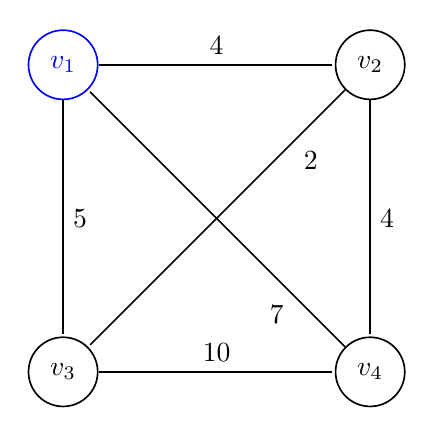
\begin{tikzpicture}[
    > = , % arrow head style
    shorten > = 1pt, % don't touch arrow head to node
    auto,
    node distance = 3cm, % distance between nodes
    semithick % line style
    ]

    \tikzset{every state}=[
    draw = black,
    thick,
    fill = white,
    minimum size = 1mm
    ]
    \node[state,blue] (v1) {$v_1$};
    \node[state] (v2) [right=of v1] {$v_2$};
    \node[state] (v3) [below =of v1] {$v_3$};
    \node[state] (v4) [below =of v2] {$v_4$};
  
    \path[->] (v1) edge  node[]{4}(v2);
    \path[->] (v1) edge  node[]{5}(v3);
    \path[->] (v2) edge  node[pos=0.2,below right]{2} (v3);
    \path[->] (v3) edge  node[]{10}(v4);
    \path[->] (v2) edge  node[]{4}(v4);
    \path[->] (v4) edge  node[pos=0.2,below left]{7}(v1);
\end{tikzpicture}
\\\\
\underline{Step 2:}\\\\
Edge $\{v_1, v_2\}$ is chosen because it has the least weight amongst all edges that $v_1$ is adjacent to. Therefore, move to $v_2$ and mark $v_2$ as visited.\\\\
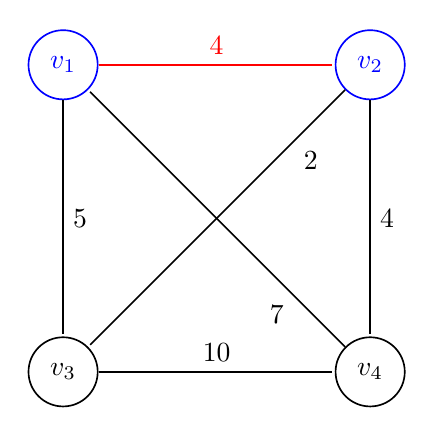
\begin{tikzpicture}[
    > = , % arrow head style
    shorten > = 1pt, % don't touch arrow head to node
    auto,
    node distance = 3cm, % distance between nodes
    semithick % line style
    ]

    \tikzset{every state}=[
    draw = black,
    thick,
    fill = white,
    minimum size = 1mm
    ]
    \node[state,blue] (v1) {$v_1$};
    \node[state, blue] (v2) [right=of v1] {$v_2$};
    \node[state] (v3) [below =of v1] {$v_3$};
    \node[state] (v4) [below =of v2] {$v_4$};
  
    \path[->] (v1) edge[red]  node[]{4}(v2);
    \path[->] (v1) edge  node[]{5}(v3);
    \path[->] (v2) edge  node[pos=0.2,below right]{2} (v3);
    \path[->] (v3) edge  node[]{10}(v4);
    \path[->] (v2) edge  node[]{4}(v4);
    \path[->] (v4) edge  node[pos=0.2,below left]{7}(v1);
\end{tikzpicture}
\\\\
\underline{Step 3:}\\\\
Since not all vertices are visited, steps 1 and 2 above are repeated and thus, edge $\{v_2, v_3\}$ is chosen. Therefore, move to vertex $v_3$ and mark $v_3$ as visited.\\\\
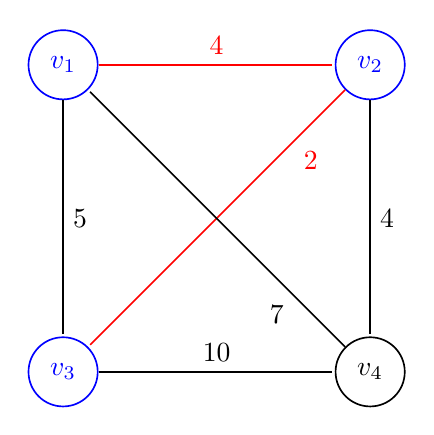
\begin{tikzpicture}[
    > = , % arrow head style
    shorten > = 1pt, % don't touch arrow head to node
    auto,
    node distance = 3cm, % distance between nodes
    semithick % line style
    ]

    \tikzset{every state}=[
    draw = black,
    thick,
    fill = white,
    minimum size = 1mm
    ]
    \node[state,blue] (v1) {$v_1$};
    \node[state,blue] (v2) [right=of v1] {$v_2$};
    \node[state,blue] (v3) [below =of v1] {$v_3$};
    \node[state] (v4) [below =of v2] {$v_4$};
  
    \path[->] (v1) edge[red]  node[]{4}(v2);
    \path[->] (v1) edge  node[]{5}(v3);
    \path[->] (v2) edge[red]  node[pos=0.2,below right]{2} (v3);
    \path[->] (v3) edge  node[]{10}(v4);
    \path[->] (v2) edge  node[]{4}(v4);
    \path[->] (v4) edge  node[pos=0.2,below left]{7}(v1);
\end{tikzpicture}
\\\\
\underline{Step 4:}\\\\
Since not all vertices are visited, steps 1 and 2 above are repeated and thus, edge $\{v_3, v_4\}$ is chosen. Therefore, move to vertex $v_4$ and mark $v_4$ as visited.\\\\
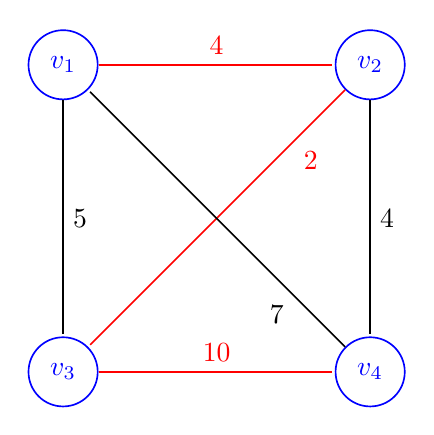
\begin{tikzpicture}[
    > = , % arrow head style
    shorten > = 1pt, % don't touch arrow head to node
    auto,
    node distance = 3cm, % distance between nodes
    semithick % line style
    ]

    \tikzset{every state}=[
    draw = black,
    thick,
    fill = white,
    minimum size = 1mm
    ]
    \node[state,blue] (v1) {$v_1$};
    \node[state,blue] (v2) [right=of v1] {$v_2$};
    \node[state,blue] (v3) [below =of v1] {$v_3$};
    \node[state,blue] (v4) [below =of v2] {$v_4$};
  
    \path[->] (v1) edge[red]  node[]{4}(v2);
    \path[->] (v1) edge  node[]{5}(v3);
    \path[->] (v2) edge[red]  node[pos=0.2,below right]{2} (v3);
    \path[->] (v3) edge[red]  node[]{10}(v4);
    \path[->] (v2) edge  node[]{4}(v4);
    \path[->] (v4) edge  node[pos=0.2,below left]{7}(v1);
\end{tikzpicture}
\\\\
\underline{Step 5:}\\\\
Since all vertices are visited, the NNA moves to the starting vertex.\\\\
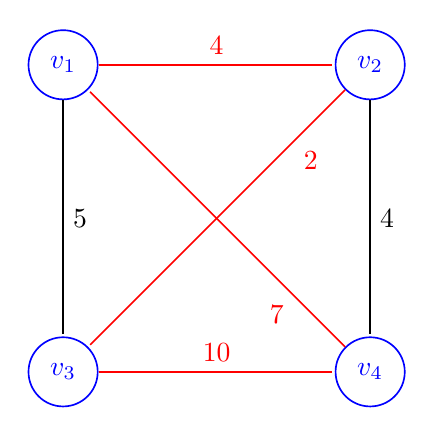
\begin{tikzpicture}[
    > = , % arrow head style
    shorten > = 1pt, % don't touch arrow head to node
    auto,
    node distance = 3cm, % distance between nodes
    semithick % line style
    ]

    \tikzset{every state}=[
    draw = black,
    thick,
    fill = white,
    minimum size = 1mm
    ]
    \node[state,blue] (v1) {$v_1$};
    \node[state,blue] (v2) [right=of v1] {$v_2$};
    \node[state,blue] (v3) [below =of v1] {$v_3$};
    \node[state,blue] (v4) [below =of v2] {$v_4$};
  
    \path[->] (v1) edge[red]  node[]{4}(v2);
    \path[->] (v1) edge  node[]{5}(v3);
    \path[->] (v2) edge[red]  node[pos=0.2,below right]{2} (v3);
    \path[->] (v3) edge[red]  node[]{10}(v4);
    \path[->] (v2) edge  node[]{4}(v4);
    \path[->] (v4) edge[red]  node[pos=0.2,below left]{7}(v1);
\end{tikzpicture}\\\\
Finally, the NNA returns the Hamiltonian cycle $v_1$, $v_2$, $v_3$, $v_4$, $v_1$ of weight 23.
\end{example}
It is important to note that in Example \ref{example_nna_explanation}, the minimum weight Hamiltonian cycle was not found. In fact, according to Example \ref{example_2.1}, the solution for the TSP given $G$ is the Hamiltonian cycle $v_1$, $v_3$, $v_2$, $v_4$, $v_1$ of weight 18. Note that the NNA would have found the optimal solution if it had started from vertex $v_2$. Since the approximate solution value does not differ a lot from the optimal value, this example seems to indicate that the NNA returns good approximations. However, this is not the case because, there could be instances where the NNA returns very bad approximations. The following example shows when the NNA can give bad approximations.
\begin{example}
\label{nna_fail}
\normalfont{Let} $M \in \mathbb{Z}^+$. Consider the graph $G$ below:
\\\\
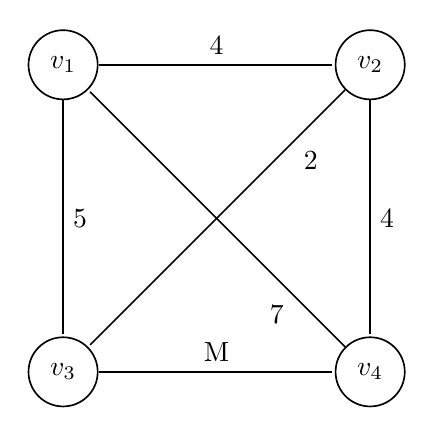
\begin{tikzpicture}[
    > = , % arrow head style
    shorten > = 1pt, % don't touch arrow head to node
    auto,
    node distance = 3cm, % distance between nodes
    semithick % line style
    ]

    \tikzset{every state}=[
    draw = black,
    thick,
    fill = white,
    minimum size = 1mm
    ]
    \node[state] (v1) {$v_1$};
    \node[state] (v2) [right=of v1] {$v_2$};
    \node[state] (v3) [below =of v1] {$v_3$};
    \node[state] (v4) [below =of v2] {$v_4$};
  
    \path[->] (v1) edge[]  node[]{4}(v2);
    \path[->] (v1) edge  node[]{5}(v3);
    \path[->] (v2) edge[]  node[pos=0.2,below right]{2} (v3);
    \path[->] (v3) edge[]  node[]{M}(v4);
    \path[->] (v2) edge  node[]{4}(v4);
    \path[->] (v4) edge[]  node[pos=0.2,below left]{7}(v1);
\end{tikzpicture}\\\\
Assuming that $M$ is a very large number, the minimum weight Hamiltonian cycle of $G$ is $v_2, v_3, v_1, v_4, v_2$ of weight 18. This minimum weight Hamiltonian cycle is found if the NNA starts from vertex $v_2$. Now suppose that the NNA starts from vertex $v_1$. Then, NNA returns the Hamiltonian cycle $v_1$, $v_2$, $v_3$, $v_4$, $v_1$ of weight $M + 13$. This means that, since $M$ is a very large number, the NNA would return an approximate result that differs a lot in weight compared to the optimal solution. Therefore, in this case, the NNA returns a very bad approximation.
\end{example}
It can be concluded from Example \ref{nna_fail} that the quality of the result returned by the NNA depends heavily on which vertex the algorithm starts with, especially when the weights differ a lot. As seen in Example \ref{nna_fail}, this happens when the edge with a very large weight has to be used in order to complete the Hamiltonian cycle, or when all other vertices have been visited. In fact in Example \ref{nna_fail}, edge $\{v_3, v_4\}$ has to be used because, $current\_vertex$ was equal to $v_3$ but only $v_4$ was unvisited.\\\\
Since the NNA is an approximation algorithm, it is natural to ask what is it's approximation ratio when applied to the TSP. As discussed in Section 2.0, we can already confirm from Theorem \ref{no_approx_tsp} that it is known that the NNA does not have a constant approximation ratio unless P=NP. As a result, the approximation ratio of the NNA applied to the TSP defined in Definition \ref{TSP} is not known, otherwise, P=NP. However, Rosenkrantz, Stearns and Lewis \cite{Rosenkrantz}, proved that, the NNA applied to an instance $G$ of the Metric-TSP has an approximation ratio that is logarithmic in the number of vertices in $G$. In what follows, a lemma will be proved. This will help in proving that the approximation ratio of the NNA applied to an instance $G$ of the Metric-TSP, is logarithmic in the number of vertices in $G$ . 
\begin{lemma}
\label{to_proove_bound}
Let G(V,E,f) be a complete weighted graph on $n$ vertices, and $W^\star$ be the optimal value of the Metric-TSP defined on G. Suppose that there exists a mapping g : V $\mapsto$ $\real^+$ such that, for all v $\in$ V, g(v) = $l_v$ and that the following  two conditions hold:
\begin{itemize}
\item $f(\{u, v\})$ $\geq$ min( $l_u$, $l_v$) for all $u$,$v$ $\in$ $V$
\item $l_u$ $\leq$ $\frac{1}{2}W^\star$ for all u $\in$ V
\end{itemize}
Then $\sum_{u \in V} l_u \leq \frac{1}{2}(\lceil log_2 n \rceil + 1)W^\star$. {\normalfont{\cite{Rosenkrantz}}}
\end{lemma}
\begin{proof}
Let $G(V,E,f)$ be a complete weighted graph on $n$ vertices, satisfying all the conditions in the Theorem statement. Suppose that $V=\{i | 1 \leq i \leq n\}$ and that, for all $i$, $j$ $\in$ V, if $i$ $\leq$ $j$ then $l_i$ $\geq$ $l_j$. Clearly, this just re-names and re-orders the vertices, hence, the generality of the proof is not effected.
\begin{claim}
\label{claim1}
$W^\star$ $\geq$ 2 $\sum_{i = k+1}^{min(2k, n)} l_i$, for all 1 $\leq$ $k$ $\leq$ n, where $k$ $\in$ $\mathbb{N}$.
\end{claim}
Let $H(V^\prime,E^\prime,f)$ be the complete weighted subgraph of $G$, such that, $V^\prime$ = $\{i | 1 \leq i \leq min(2k, n)\}$. Let $T$ be a sequence of vertices representing a Hamiltonian cycle in $H$, such that, the vertices are ordered as they would appear in a minimum weight Hamiltonian cycle of $G$. Let $C(V^\prime, E^{\prime\prime}, f)$ be the Cycle graph obtained from $T$ with weight $T^\star$. By the triangle inequality, for all $\{i, j\}$ $\in$ $E^{\prime\prime}$, $f(\{i, j\})$ is less than or equal to the weight of the path from $i$ to $j$ in a minimum weight Hamiltonian cycle of $G$. This holds because, the vertices in $T$ appear in the same order as in the minimum weight Hamiltonian cycle. Therefore, $T^\star$ $\leq$ $W^\star$. Now, by Definition \ref{weightofasubgraph}, $T^\star$ =  $\sum_{\{i, j\} \in E^{\prime\prime}} f(\{i, j\})$. Therefore, by the first bullet point in Lemma \ref{to_proove_bound},  $T^\star$ = $\sum_{\{i, j\} \in E^{\prime\prime}} f(\{i, j\})$ $\geq$  $\sum_{\{i, j\} \in E^{\prime\prime}} min(l_i, l_j)$. For each $i$ $\in$ [$min(2k, n)$], let $\alpha_i$ be the number of edges $\{i, j\}$ $\in$ $E^{\prime\prime}$, such that, $i > j$ ( i.e $l_i$ = $min(l_i, l_j)$). Then, $\sum_{\{i, j\} \in E^{\prime\prime}} min(l_i, l_j)$ = $\sum_{i \in E^\prime} \alpha_il_i$\\
$\implies$ $T^\star$ $\geq$ $\sum_{i \in E^\prime} \alpha_i l_i$ = $\sum_{i =1}^{min(2k, n)} \alpha_i l_i$.\\ Now, for all $i$ $\in$ [$min(2k, n)$], $\alpha_i$ $\leq$ 2. This is true because, every vertex $v_i$ is incident to exactly two edges of $C$. In addition to this, $\alpha_1$ + .. + $\alpha_{min(2k, n)}$ = $\abs{E^{\prime\prime}}$, because, for all $\{i,j\}$ $\in$ $E^{\prime\prime}$, either $ i \geq j$ or $j > i$. Therefore, either $\alpha_i$ or $\alpha_j$ is incremented by one. Another observation is that, $k$ is at least half of the number of vertices in $C$. This is true because of the following. Suppose that, $min(2k, n)$ = 2k. Then, by the construction of $C$ and $H$, $C$ contains $2k$ vertices. Hence, $k$ must be half of the number of vertices in $C$. Now, suppose that $min(2k, n)$ = $n$. Then, by the construction of $C$ and $H$, $C$ contains $n$ vertices. Now, $n$ $\leq$ $2k$, hence, $k$ must be at least half of the number of vertices in $C$. Therefore, from both cases, it can be deduced that $k$ is at least half of the number of vertices in $C$.
\begin{claim}
\label{claim2}
$\sum_{i =1}^{min(2k, n)} \alpha_i l_i$ $\geq$ 2 $\sum_{i = k + 1}^{min(2k, n)} l_i$.
\end{claim}
Since $k$ is at least half the number of vertices in $C$, and each $l_i$ is positive, 2 $\sum_{i = k + 1}^{min(2k, n)} l_i$ has the largest value when $k$ = $\frac{1}{2} min(2k, n)$. Therefore, if we can prove Claim \ref{claim2} for $k$ = $\frac{1}{2} min(2k, n)$, we prove it for all possible $k$. Let $k$ = $\frac{1}{2} min(2k, n)$ and $\alpha_i$ = 2 for all $i$ $\in$ [$k+1,min(2k, n)$]. Then, $\alpha_{k+1}$ + ... + $\alpha_{min(2k, n)}$ = 2($min(2k, n)$ - $k$) = 2($min(2k, n)$ -  $\frac{1}{2} min(2k, n)$ ) =  $min(2k, n)$ = number of edges in $C$. Therefore, since $\alpha_1$ + .. + $\alpha_{min(2k, n)}$ = $\abs{E^{\prime\prime}}$, then, $\alpha_i$ = 0 for all $i$ $\in$ [$k$]. Therefore, $\sum_{i =1}^{min(2k, n)} \alpha_i l_i$ = $\sum_{i = k + 1}^{min(2k, n)}2 l_i$ = 2 $\sum_{i = k + 1}^{min(2k, n)} l_i$. Therefore $\sum_{i =1}^{min(2k, n)} \alpha_i l_i$ $\geq$ 2 $\sum_{i = k + 1}^{min(2k, n)} l_i$, and hence, Claim \ref{claim2} is proved.\\\\
Now, since $W^\star$ $\geq$ $T^\star$ $\geq$ $\sum_{i =1}^{min(2k, n)} \alpha_i l_i$. Then, by Claim \ref{claim2}, $W^\star$  $\geq$ 2 $\sum_{i = k + 1}^{min(2k, n)} l_i$, and hence Claim \ref{claim1} is proved aswell.\\\\
By Claim \ref{claim1},  $W^\star$  $\geq$ 2 $\sum_{i = k + 1}^{min(2k, n)} l_i$. \\Hence,  $\sum_{j = 0}^{\lceil log_2 n \rceil - 1} W^\star$  $\geq$ $\sum_{j = 0}^{\lceil log_2 n \rceil -1} 2 \sum_{i = k + 1}^{min(2k, n)} l_i$. Letting $k$ = $2^{j}$, we get that,  $\sum_{j = 0}^{\lceil log_2 n \rceil - 1} W^\star$  $\geq$ $\sum_{j = 0}^{\lceil log_2 n \rceil -1} 2 \sum_{i = 2^j + 1}^{min(2^{j+1}, n)} l_i$. \\$\implies$ $\lceil log_2 n \rceil$ $W^\star$  $\geq$ 2 $\sum_{i = 2}^{n} l_i$. Now, bullet point number two in Lemma \ref{to_proove_bound} implies that, $W^\star$ $\geq$ 2$l_1$. \\$\implies$ $\lceil log_2 n \rceil$ $W^\star$  $\geq$ 2 $\sum_{i = 1}^{n} l_i$.\\$\implies$  $\frac{1}{2}$ ($\lceil log_2 n \rceil$ + 1) $W^\star$  $\geq$ $\sum_{i = 1}^{n} l_i$ = $\sum_{u \in V} l_u$.
\end{proof}
The above proof was constructed using ideas from \cite{Rosenkrantz}. Having proved Lemma \ref{to_proove_bound}, it is now time to prove that, when applied to an instance $G$ of the Metric-TSP, the NNA has an approximation ratio that depends logarithmically on the number of vertices in $G$.
\begin{theorem}
\label{log_bound_thrm}
Suppose that $G(V,E,f)$ is an instance of the Metric-TSP. Let $W^\star$ be the optimal value of $G$, and apply the NNA on $G$. Suppose that $W$ is the value of the approximation returned by the NNA. Then, $\frac{W}{W^\star}$ $\leq$ $\frac{1}{2}(\lceil log_2 n \rceil + 1)$ {\normalfont\cite{Rosenkrantz}}.
\end{theorem}
\begin{proof}
Define $G(V,E,f)$, $W^\star$ and $W$ as stated in Theorem \ref{log_bound_thrm}. Consider the NNA Procedure described in this section and apply it to $G$. Let $g$ : $V$ $\mapsto$ $\real^+$ be a mapping defined by $g(v)$ = $f(\{v,u\})$, where, $u$ is the vertex chosen by the NNA when $current\_vertex = v$. For all $v$ $\in$ $V$, let $l_v$ = $g(v)$. We show that $g$ satisfies the two conditions of Lemma \ref{to_proove_bound}.\\\\
\textbf{Condition 1} :  $f(\{u, v\})$ $\geq$ min( $l_u$, $l_v$) for all $u$,$v$ $\in$ $V$\\\\
Let $u$, $v$ $\in$ $V$. Suppose that $u$ was set as visited by the NNA before $v$. Then, since $G$ is complete, $\{u, v\}$ was a candidate edge for the NNA when $current\_vertex$ was equal to $u$. Therefore, $f(\{u, v\})$ is greater than or equal to the weight of the edge selected when $current\_vertex$ was equal to $u$. Note that the weight of the selected edge is $l_u$. Therefore, $f(\{u, v\})$ $\geq$ $l_u$ (*). Using the same argument, if $v$ was set as visited by the NNA before $u$, then, $f(\{v, u\})$ = $f(\{u, v\})$ $\geq$ $l_v$ (**). Now, since the NNA must visit all veritices, either $u$ is visited before $v$ or vice-versa. As a result, one of (*) or (**) must hold. Hence, $f(\{u, v\})$ $\geq$ min($l_u$, $l_v$). Therefore, since $u$ and $v$ are arbitrary, Condition 1 holds.\\\\
\textbf{Condition 2} :  $l_u$ $\leq$ $\frac{1}{2}W^\star$ for all u $\in$ V\\\\
Let  $u$, $v$ $\in$ V such that, $l_u$ = $f(\{u, v\})$. Let $h$ be a minimum weight Hamiltonian cycle in $G$. Since $h$ is spanning a spanning subgraph, both $u$ and $v$ are in $h$. Therefore, $h$ can be expressed as the disjoint union of two paths joining $u$ and $v$. One of the paths can be obtain by starting from vertex $u$ and traversing through $h$ clockwise until finding $v$. The other path can be obtained by starting from vertex $u$ and traversing through $h$ anti-clockwise until finding $v$. Let these paths be $p_1$ and $p_2$. By the triangle inequality, the weight of $p_1$ and the weight of $p_2$ are both greater than or equal to $f(\{u,v\})$ in $G$. Therefore, summing both inequalities we get, 2$l_u$ = $2f(\{u,v\})$ $\leq$ weight of $p_1$ + weight of $p_2$ = weight of $h$ = $W^\star$. As a result, $l_u$ $\leq$ $\frac{1}{2}W^\star$. Therefore, since $u$ is arbitrary, Condition 2 holds.\\\\Now, for all $v$ in $V$, $l_v$ is the weight of the edge chosen by the NNA when $current\_vertex = v$. Therefore, $\sum_{u \in V} l_u $ =  $W$. Using Lemma \ref{to_proove_bound}, $W$ = $\sum_{u \in V} l_u $ $\leq$ $\frac{1}{2}$ ($\lceil log_2 n \rceil$ + 1) $W^\star$.\\ $\implies$ $W$ $\leq$ $\frac{1}{2}$ ($\lceil log_2 n \rceil$ + 1) $W^\star$\\ $\implies$ $\frac{W}{W^\star}$ $\leq$ $\frac{1}{2}$ ($\lceil log_2 n \rceil$ + 1).
\end{proof}
The proof of Theorem \ref{log_bound_thrm} was constructed using ideas in \cite{Rosenkrantz}.\\\\
The implication of Theorem \ref{log_bound_thrm} is that, when applying the NNA on an instance $G$ of the Metric-TSP, the quality of the approximation depends on the number of vertices in $G$. This is true because of the following. As the number of vertices increases, the approximation ratio increases logarithmically. Therefore, for very large $n$, $\frac{1}{2}(\lceil log_2 n \rceil + 1)$ may become very large that it may allow bad approximations to be returned by the NNA. These bad approximation would be returned because, their value would still be less than $\frac{1}{2}(\lceil log_2 n \rceil + 1)$ $\times$ optimal value. One way of solving this problem is to try and deduce whether the NNA can have a constant approximation ratio when applied to the Metric-TSP. This would solve the problem because, as the number of vertices increases, we are guaranteed that the value of the approximation is within a constant factor of the optimal value. In other words, as the number of vertices increases, approximations whose value is greater than the approximation ratio would not become eligible for the NNA. However, Rosenkrantz, Stearns and Lewis \cite{Rosenkrantz}, proved that there is an instance $G$ of the Metric-TSP such that, when the NNA is applied to $G$, it has an approximation ratio that is strictly bounded below by a logarithmic function of the number of vertices in $G$. This means that in general, the NNA cannot have a constant approximation ratio when applied to the Metric-TSP. This fact is stated in Theorem \ref{no_proof} below without proof because, the proof is too long.
\begin{theorem}
\label{no_proof}
For all m $>$ 3, m $\in$ $\mathbb{N}$, there is an instance $G(V,E,f)$ of the Metric-TSP such that, $\abs{V}$ = $2^m - 1$ and $\frac{W}{W^\star}$ $>$ $\frac{1}{3}$($log_2 (n+1))$ $+$ $\frac{4}{9}$, where $W$ is the optimal value of $G$, and $W^\star$ is the value of the approximation returned by the NNA when it is applied to $G$.{\normalfont{\cite{Rosenkrantz}}}
\end{theorem}
Theorem \ref{log_bound_thrm} and \ref{no_proof} imply that in general the NNA cannot have a constant approximation ratio when applied to the Metric-TSP. However, this does not mean that the Metric-TSP cannot be approximated using an approximation algorithm that has a constant approximation ratio. In fact, an approximation algorithm that is known to have a contstant approximation ratio when applied to the Metric-TSP is the Twice Around the Minimum Spanning Tree Approximation Algorithm. The Twice Around the Minimum Spanning Tree Approximation Algorithm will be presented in the next subsection.    
\subsubsection{Twice Around the Minimum Spanning Tree Approximation Algorithm}
\label{TAMSA_SECTION}
Similarly to the NNA, the Twice Around the Minimum Spanning Tree Algorithm (TAMSA) is an algorithm that can find near-optimal solutions for the TSP \cite{cormen_leiserson_rivest_stein}. The TAMSA computes an approximate solution for the TSP by using two other algorithms. In what follows, these two algorithms will be briefly described without delving into any specific details related to their implementation.\\\\
The first algorithm used by the TAMSA is Prim's algorithm. Prim's algorithm takes a weighted graph $G(V,E,f)$ and an arbitrary starting vertex $r$ $\in$ $V$ as inputs, and returns a minimum weight spanning tree $T(V^\prime,E^\prime,f)$ of $G$. Prim's algorithm computes $T$ in the following way. The algorithm initially starts with empty $V^\prime$ and empty $E^\prime$. Then, the algorithm proceeds by adding $r$ to $V^\prime$. Afterwards, the algorithm adds to $E^\prime$, the edge of least-weight connecting a vertex $v^\prime$ in $V^\prime$ to a vertex $v$ $\notin$ $V^\prime$. Following this, $v$ is added to $V^\prime$. The whole procedure is then repeated until all vertices in $V$ are added to $V^\prime$. \cite{harris_hirst_mossinghoff_2008}\\\\
An important question that must be answered is whether the procedure described in the previous paragraph does return a minimum weight spanning tree. Typically, one needs to show that the mathematical structure returned by Prim's algorithm is that of a spanning tree, whose weight is the least possible among all spanning trees of the input graph. Note that, the answer to this question is vital for algorithms that use Prim's algorithm to produce a minimum weight spanning tree. In fact, if Prim's algorithm does not return a minimum weight spanning tree, the algorithms that use Prim's algorithm need to use another algorithm to compute a minimum weight spanning tree. The next two theorems confirm that given an arbitrary complete weighted graph $G$ together with an arbitray starting vertex $r$ as input, Prim's algorithm always returns a minimum weight spanning tree of $G$. Theorem \ref{correctness1} was constructed using ideas from \cite{greedy_algorithms}.
\begin{theorem}
\label{correctness1}
Prim's algorithm always returns a spanning tree. {\normalfont{\cite{prim's_algorithm}}}
\end{theorem}
\begin{proof}
Let $G(V,E,f)$ be a complete weighted graph, and $T(V^\prime,E^\prime,f)$ be the graph returned by Prim's algorithm when given $G$ and an arbitrary vertex $s$ $\in$ $V$ as input. Note that $s$ is the starting vertex for Prim's algorithm. To show that $T$ is a spanning tree, it must be shown that $T$ is a connected spanning sub graph of $G$ with no cycles. Note that $T$ is a sub graph of $G$ because, Prim's algorithm constructs $T$ using vertices and edges that belong to $G$.\\\\
Suppose that $T$ does not span $G$. Then, there exists a non-empty set of vertices $X$ $\subseteq$ $V$ such that, $X$ $\cap$ $V^\prime$ = $\emptyset$. Let $x$ $\in$ $X$. Then, $x$ $\notin$ $V^\prime$ and hence, there are no edges in $E$ of the form $\{v,x\}$ where $v$ $\in$ $V^\prime$, otherwise, Prim's algorithm would have chosen the edge and added $x$ to $V^\prime$. Now, since $G$ is connected, there exists a path $P$ in $G$ joining $s$ to $x$. In addition to this, $s$ $\in$ $V^\prime$ and $x$ $\in$ $X$. Hence, $P$ must contain an edge of the form $\{v, x\}$, where $v$ $\in$ $V^\prime$. This means that $E$ contains an edge of the form $\{v, x\}$, where $v$ $\in$ $V^\prime$. Contradiction. Therefore, $T$ must be a spanning sub graph of $G$.\\\\
To show that $T$ is connected, it must be shown that any two distinct vertices in $V^\prime$ are connected by a path. Let $u$, $v$ $\in$ $V^\prime$ such that, $u$ $\neq$ $v$. Now, before Prim's algorithm adds $u$ to $V^\prime$, it connects it with a vertex $u_k$ which is already in $V^\prime$. But before $u_k$ was added to $V^\prime$, Prim's algorithm must have connected $u_k$ to a vertex $u_{k-1}$ that is already in $V^\prime$. Repeat this argument until reaching a vertex $z$, which is not connected to another vertex from a previous iteration of Prim's algorithm. Note that a vertex $z$ exists because, since there are a finite number of vertices in $V$, there are a finite number of vertices in $V^\prime$ that could have been chosen before $u$. From the description of Prim's algorithm above, this argument terminates when $z$ = $s$. This is true because, $s$ is the only vertex in $V$ which was not connected to another vertex in $V^\prime$ prior to being added to $V^\prime$. Now, suppose that $k$ vertices were added to $V^\prime$ before $u$. Then, $s= u_0, u_1, u_2, ..., u_k, u_{k+1} = u$ must be a path in $T$ joining $s$ to $u$ because, $\{u_i, u_{i+1}\}$ $\in$ $E^\prime$ for all $i$ $\in$ [$k$]. Now, the same argument can be repeated for $v$ and hence, $s$ and $v$ must also be connected by a path $P^\prime$. Therefore, since both $u$ and $v$ connect to the same vertex $s$ via a path, we can start from a vertex $u$ ($v$), travel to $s$ using $P$ ($P^\prime$), and travel to $v$ using $P^\prime$ ($P$). Therefore, $u$ and $v$ must be connected by a path. Hence, $T$ must be a connected spanning sub graph of $G$.\\\\
Suppose that $T$ contains a cycle $C$. Let $\{c_1, c_2\}$ be the last edge of $C$ that was added by Prim's algorithm to $E^\prime$ (hence the edge that caused the cycle to be created). WLOG, suppose that $c_1$ was added to $V^\prime$ by Prim's algorithm before $c_2$. Then, since Prim's algorithm adds an edge between a vertex in $V^\prime$ and a vertex not in $V^\prime$, it must be that $c_2$ is not in $V^\prime$ before $\{c_1, c_2\}$ is added to $E^\prime$. Hence, before $\{c_1, c_2\}$ is added to $E^\prime$, there are no paths in $T$ joining $c_1$ to $c_2$. This means that, no cycle is created when adding $\{c_1, c_2\}$ to $E^\prime$ because, $c_1$ would be connected to $c_2$ by exactly one path (the path $c_1, c_2$). Contradiction, since $\{c_1, c_2\}$ is the edge that caused the cycle to be created. Therefore, $T$ must be a connected spanning sub graph of $G$ without cycles, hence, by Definition \ref{spanning tree}, $T$ is a spanning tree of $G$.
\end{proof}
Theorem \ref{correctness1} confirms that Prim's algorithm returns a spanning tree. Now, it must be shown that the spanning tree returned by Prim's algorithm has the least possible weight among all spanning trees of $G$. Theorem \ref{correctness2} was adapted using ideas from \cite{prim's_algorithm}.
\begin{theorem}
Prim's algorithm always returns a minimum weight spanning tree. {\normalfont{\cite{prim's_algorithm}}}
\label{correctness2}
\end{theorem}
\begin{proof}
Let $G(V,E,f)$ be a complete weighted graph, and $T(V^\prime,E^\prime,f)$ be the spanning tree returned by Prim's algorithm when given $G$ and an arbitrary vertex $s$ $\in$ $V$ as input. Note that, $s$ is the starting vertex for Prim's algorithm. Let $T^\star(V^\star,E^\star,f)$ be a minimum weight spanning tree of $G$. If $T$ = $T^\star$, the theorem holds.\\\\
Suppose that $T$ $\neq$ $T^\star$. Then,  $E^\prime$ $\setminus$ $E^\star$ $\neq$ $\emptyset$. Let $e = \{v_1, v_2\}$ $\in$  $E^\prime$ $\setminus$ $E^\star$. Let $S$ $\subset$ $V^\prime$ be the set of vertices in $V^\prime$ just before Prim's algorithm adds the edge $\{v_1, v_2\}$ to $E^\prime$. Although $e$ $\notin$ $E^\star$, there is a path $P$ joining $v_1$ to $v_2$ in $T^\star$, because, $T^\star$ is a spanning tree. Now, by construction of $S$, $v_1$ $\in$ $S$ and $v_2$ $\notin$ $S$. Hence, P is a sequence of vertices beginning with vertices in $S$, and ending with vertices which are not in $S$. Therefore, there exists some edge $e^\prime = \{x,y\}$ $\in$ $E^\star$ such that $x$ $\in$ $S$ and $y$ $\notin$ $S$. Now, in the iteration of Prim's algorithm when $V^\prime$ = $S$, both $e$ and $e^\prime$ connect a vertex which is in $V^\prime$ to a vertex which is not in $v^\prime$. Hence, both $e$ and $e^\prime$ are eligible to be chosen by Prim's algorithm at this stage. However, it is known that $e$ is chosen instead of $e^\prime$. This means that, $e$ is an edge of lesser weight than $e^\prime$. Now, if the edge $e^\prime$ is removed from $E^\star$ and replaced with the edge $e$, we get a path $P^{\prime\prime}$ in $T^\star$ joining $x$ to $y$. Hence, ($T^\star$ $\setminus$ $P$) $\cup$ $P^{\prime\prime}$ would still remain a spanning tree. Let $T^\sim$ be the spanning tree ($T^\star$ $\setminus$ $P$) $\cup$ $P^{\prime\prime}$. Then, $T^\sim$ differs from $T^\star$ exactly in the edges $e$ and $e^\prime$, where, $f(e)$ $\geq$ $f(e^\prime)$. This means that, $T^\sim$ has weight at most that of $T^\star$. Now, since $T^\star$ is a minimum spanning tree, it must be a spanning tree of least weight. Hence, $f(T^\sim)$ = $f(T^\star)$. Therefore, if this procedure is repeated for every edge in $E^\prime$ $\setminus$ $E^\star$, $T^\star$ would be converted into a spanning tree $W^\prime = T$, where $f(T) = f(W^\prime) = f(T^\star)$. Therefore, $T$ must be a minimum weight spanning tree. Note that this holds because, the procedure can be repeated only for a finite number of times. This is true because, since $G$ is a finite graph, $|E^\prime$ $\setminus$ $E^\star|$ is a finite number.
\end{proof}
What follows is an example that demonstrates how Prim's algorithm constructs a minimum weight spanning tree of a graph.
\begin{example}
\label{example_prim}
\normalfont{Consider} the graph $G$ in Example \ref{example4}, and the brief description of Prim's algorithm. Let $T(V^\prime,E^\prime)$ be the graph with an empty set of vertices, and an empty set of edges. Assuming that the starting vertex is $v_1$, Prim's algorithm starts by adding $v_1$ to $V^\prime$. Hence $T$ is now the following graph:\\\\
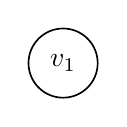
\begin{tikzpicture}[
    > = , % arrow head style
    shorten > = 1pt, % don't touch arrow head to node
    auto,
    node distance = 3cm, % distance between nodes
    semithick % line style
    ]

    \tikzset{every state}=[
    draw = black,
    thick,
    fill = white,
    minimum size = 1mm
    ]
    \node[state] (v1) {$v_1$};
\end{tikzpicture}\\\\
The algorithm now proceeds by adding the edge of least weight from $E$ to $E^\prime$, which connects a vertex $v^\prime$ $\in$ $V^\prime$ to a vertex $v$ $\notin$ $V^\prime$. Also, $v$ is added to $V^\prime$. In this example, these properties are satisfied by the edge $\{v_1, v_2\}$, hence, $T$ is the following graph.\\\\
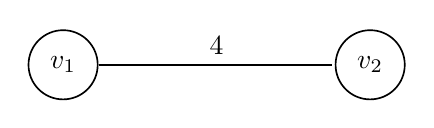
\begin{tikzpicture}[
    > = , % arrow head style
    shorten > = 1pt, % don't touch arrow head to node
    auto,
    node distance = 3cm, % distance between nodes
    semithick % line style
    ]

    \tikzset{every state}=[
    draw = black,
    thick,
    fill = white,
    minimum size = 1mm
    ]
    \node[state] (v1) {$v_1$};
    \node[state] (v2) [right=of v1] {$v_2$};
  
    \path[->] (v1) edge[]  node[]{4}(v2);
\end{tikzpicture}\\\\
Since not all vertices in $V$ have been added to $V^\prime$, the same procedure is repeated. Hence, the edge $\{v_2, v_3\}$ is chosen because, it is the edge of least weight connecting a vertex in $V^\prime$ to a vertex not in $V^\prime$. Therefore, $T$ is the following graph\\\\
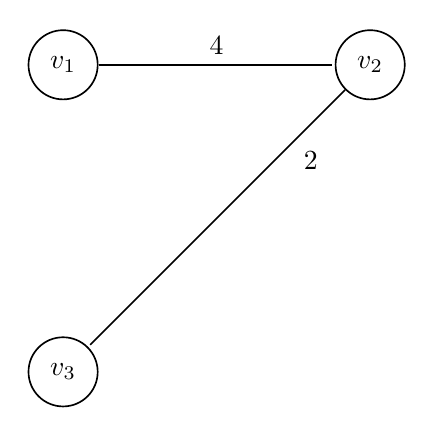
\begin{tikzpicture}[
    > = , % arrow head style
    shorten > = 1pt, % don't touch arrow head to node
    auto,
    node distance = 3cm, % distance between nodes
    semithick % line style
    ]

    \tikzset{every state}=[
    draw = black,
    thick,
    fill = white,
    minimum size = 1mm
    ]
    \node[state] (v1) {$v_1$};
    \node[state] (v2) [right=of v1] {$v_2$};
    \node[state] (v3) [below =of v1] {$v_3$};
  
    \path[->] (v1) edge[]  node[]{4}(v2);
    \path[->] (v2) edge[]  node[pos=0.2,below right]{2} (v3);
\end{tikzpicture}\\\\
Again, since not all vertices in $V$ have been added to $V^\prime$, the same procedure is repeated. In this case, $\{v_2, v_4\}$ is the edge of least weight connecting a vertex in $V^\prime$ to a vertex not in $V^\prime$. Therefore, $T$ is the following graph.\\\\
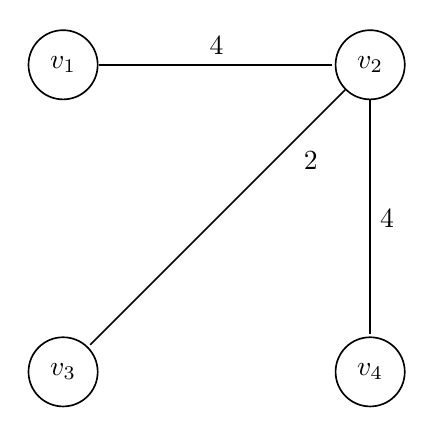
\begin{tikzpicture}[
    > = , % arrow head style
    shorten > = 1pt, % don't touch arrow head to node
    auto,
    node distance = 3cm, % distance between nodes
    semithick % line style
    ]

    \tikzset{every state}=[
    draw = black,
    thick,
    fill = white,
    minimum size = 1mm
    ]
    \node[state] (v1) {$v_1$};
    \node[state] (v2) [right=of v1] {$v_2$};
    \node[state] (v3) [below =of v1] {$v_3$};
    \node[state] (v4) [below =of v2] {$v_4$};
  
    \path[->] (v1) edge[]  node[]{4}(v2);
    \path[->] (v2) edge[]  node[pos=0.2,below right]{2} (v3);
    \path[->] (v2) edge  node[]{4}(v4);
\end{tikzpicture}\\\\
Since all vertices in $V$ have been added to $V^\prime$, the algorithm now terminates by returning $T$.
\end{example}
The second algorithm used by the TAMSA is the preorder tree walk algorithm, more commonly known as the depth first traversal tree algorithm. Given a tree $T(V,E,f)$ and an arbitrary starting vertex $r$ $\in$ $V$ as inputs, the preorder tree walk algorithm returns a walk $S$ of $T$ containing all vertices in $V$, where the vertices are ordered according to how they were visited while performing the walk. The preorder tree walk algorithm computes a walk $S$ in the following way. At the start of the algorithm, $S$ is empty. Then, starting from $r$, the algorithm marks $r$ as visited and adds $r$ to $S$. Following this, the algorithm recursively calls itself on all unvisited neighbors of $r$. The entire procedure is repeated until all vertices in $V$ are added to $S$. Note that in this section, the execution of the preorder tree walk algorithm on an arbitrary tree will be termed as a preorder walk. For example, a preorder walk of the tree in Figure \ref{tree_example} below, results in the vertex sequence $v_1, v_2, v_3, v_4, v_5, v_9, v_6, v_7, v_8$. \cite{cormen_leiserson_rivest_stein}\\\\
\begin{figure}[h]
\centering
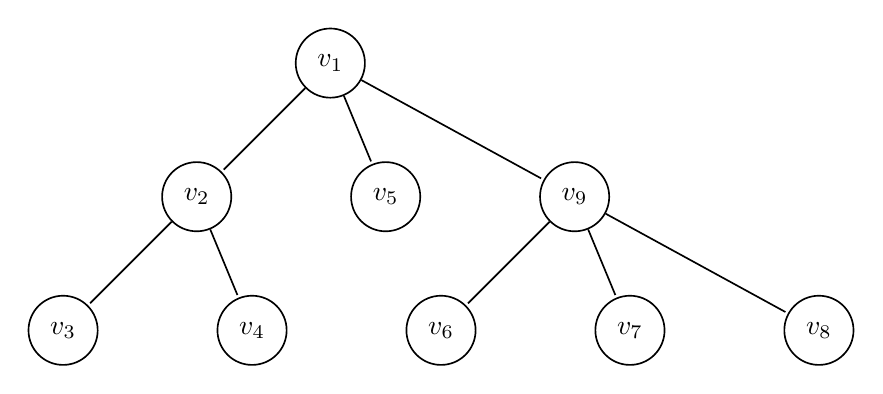
\begin{tikzpicture}[
    > = , % arrow head style
    shorten > = 1pt, % don't touch arrow head to node
    auto,
    node distance = 1.5cm, % distance between nodes
    semithick, % line style
    ]

    \tikzset{every state}=[
    draw = black,
    thick,
    fill = white,
    minimum size = 1mm
    ]
    \node[state] (v1) {$v_1$};
    \node[state] (v2) [below left=of v1] {$v_2$};
    \node[state] (v5) [right=of v2] {$v_5$};
    \node[state] (v9) [right =of v5] {$v_9$};
    \node[state] (v3) [below left =of v2]{$v_3$};
    \node[state] (v4) [right=of v3] {$v_4$};
    \node[state] (v6) [below left =of v9] {$v_6$};
    \node[state] (v7) [right=of v6] {$v_7$};
    \node[state] (v8) [right =of v7] {$v_8$};
  
    \path[->] (v1) edge[]  node[]{}(v2);
    \path[->] (v2) edge[]  node[]{} (v3);
    \path[->] (v2) edge  node[]{}(v4);
    \path[->] (v1) edge[]  node[]{}(v5);
    \path[->] (v1) edge[]  node[]{} (v9);
    \path[->] (v9) edge  node[]{}(v6);
    \path[->] (v9) edge  node[]{}(v7);
    \path[->] (v9) edge  node[]{}(v8);
\end{tikzpicture}
\caption{Tree example}
\label{tree_example}
\end{figure}\\\\
Having briefly described important algorithms that will be used by the TAMSA algorithm, now it is time to describe the TAMSA itself. The TAMSA takes an instance of the TSP as input, and returns a sequence of vertices representing a Hamiltonian cycle \cite{cormen_leiserson_rivest_stein}. The TAMSA algorithm can be described using the pseudo code below which was adapted from \cite{cormen_leiserson_rivest_stein}.\\\\
\textbf{TAMSA($G(V,E,f)$):}
\begin{itemize}
\itemsep0em
\item Choose an arbitrary vertex $r$ $\in$ V as starting vertex.
\item Starting from $r$, compute a minimum weight spanning tree $T$ of $G$ using Prim's algorithm.
\item Perform a preorder walk on T starting from $r$, and let $S$ be the walk returned by the preorder tree walk algorithm.
\item Add $r$ to $S$ as a final vertex and return S.
\end{itemize}
For the TAMSA to be a useful approximation algorithm that approximates the TSP, it must guarantee that it will return a Hamiltonian cycle, and that the Hamiltonian cycle is computed in polynomial time. Let $G$ be an instance of the TSP, and let $T$ be the minimum weight spanning tree of $G$ returned by Prim's algorithm. By Theorem \ref{correctness2} and Theorem \ref{correctness1} it is guaranteed that $T$ is a minimum weight spanning tree. Now, let $S$ be the sequence of vertices returned by a preorder walk on $T$. Since $T$ has no cycles and, visited vertices can never be visited again, a preorder tree walk of $T$ can never result into a walk with repetition of vertices. Hence, $S$ has no repetition of vertices. In addition to this, since $T$ is connected, the preorder tree walk algorithm terminates when all vertices of $G$ have been added to $S$. Therefore, $S$ must contain all vertices of $G$. Hence, $S$ must be a path containing all vertices of $G$. As a result, for $S$ to be a Hamiltonian cycle, the first vertex in $S$ must be repeated as a final vertex. This is done by bullet point number four in the TAMSA pseudo code. Therefore, it can be concluded that $S$ must be a Hamiltonian cycle. The next step is to check that the TAMSA computes a Hamiltonian cycle in polynomial time.\\\\
Given a TSP instance $G(V,E,f)$, the time complexity of the TAMSA is $O(|V|^2)$ \cite{cormen_leiserson_rivest_stein}. This is true because of the following. Consider the TAMSA pseudo code above. Clearly, the largest amount of work to be performed by the TAMSA is to compute a minimum weight spanning tree $T$ of $G$, and to compute a preorder tree walk of $T$. The preorder tree walk of $T$ takes $O(|V|)$ steps because, the preorder tree walk algorithm terminates when all the vertices in $G$ have been visited (this is true due to reasons mentioned in the previous paragraph). Hence, bullet point number three takes $O(|V|)$ time. Now, according to Exercise 23.2-2 in \cite{cormen_leiserson_rivest_stein}, there is an implementation of Prim's algorithm that takes $O(|V^2|)$ time in order to compute a minimum weight spanning tree. Thus, the total time complexity of the TAMSA is $O(|V^2|)+ O(|V|) = O(|V^2|)$. However, in \cite{cormen_leiserson_rivest_stein} it is shown that the asymptotic time complexity of Prim's algorithm can be improved to $O(|E| log(|V|))$ by using a binary min-heap. This would mean that the time complexity of the TAMSA is no longer $O(|V^2|)$, but is $O(|E| log(|V|))$. As a result, the TAMSA has a log-linear time complexity. Therefore, using Table \ref{tab:table1} in Section 1.2, and and the fact that the NNA has a quadratic time complexity (discussed in Section 2.1.1), the TAMSA is more efficient asymptotically because, it has a smaller order of growth. Note that, the analysis of the time complexity of Prim's algorithm is not given because, it requires theory about data structures such as Heaps to be established, and this is out of the scope of this project. What follows is an example which demonstrates how the TAMSA computes a Hamiltonian cycle.
\begin{example}
\label{tamsa_demonstration}
\normalfont{Consider} the graph $G$ in Example \ref{example4}, and the TAMSA pseudo code presented in this section. Assume that randomly, the TAMSA chooses vertex $v_1$ as starting vertex. From Example \ref{example_prim}, the minimum spanning tree $T$ returned by Prim's algorithm starting from vertex $v_1$ is the graph below.\\\\
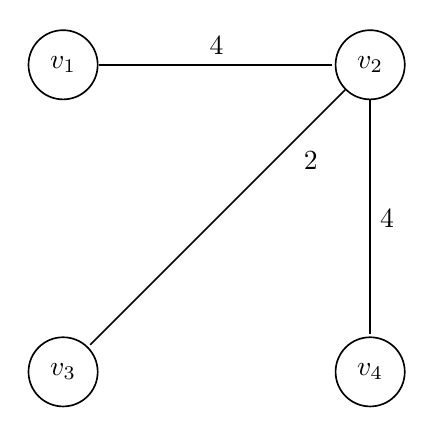
\begin{tikzpicture}[
    > = , % arrow head style
    shorten > = 1pt, % don't touch arrow head to node
    auto,
    node distance = 3cm, % distance between nodes
    semithick % line style
    ]

    \tikzset{every state}=[
    draw = black,
    thick,
    fill = white,
    minimum size = 1mm
    ]
    \node[state] (v1) {$v_1$};
    \node[state] (v2) [right=of v1] {$v_2$};
    \node[state] (v3) [below =of v1] {$v_3$};
    \node[state] (v4) [below =of v2] {$v_4$};
  
    \path[->] (v1) edge[]  node[]{4}(v2);
    \path[->] (v2) edge[]  node[pos=0.2,below right]{2} (v3);
    \path[->] (v2) edge  node[]{4}(v4);
\end{tikzpicture}\\\\
Now, according to bullet point number three in the TAMSA pseudo code, the TAMSA must perform a preorder tree walk on $T$. Consider the brief description of the preorder tree walk algorithm. A preorder walk of $T$ is computed in the following way. Note that, in the following demonstration, the blue vertices are the vertices that have already been visited by the preorder tree walk algorithm, and the black vertices are those vertices that have not yet been visited by the preorder tree walk algorithm.\\
The algorithm starts by visiting the starting vertex $v_1$ and adding it to $S$. Therefore, $S = v_1$.
\\\\
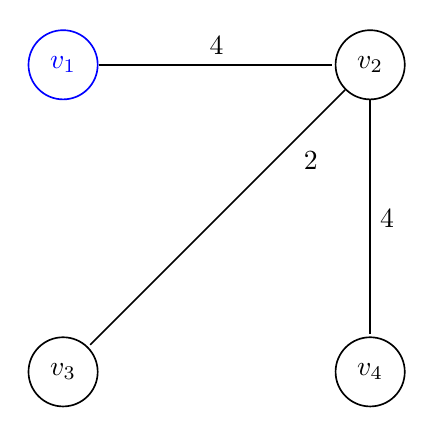
\begin{tikzpicture}[
    > = , % arrow head style
    shorten > = 1pt, % don't touch arrow head to node
    auto,
    node distance = 3cm, % distance between nodes
    semithick % line style
    ]

    \tikzset{every state}=[
    draw = black,
    thick,
    fill = white,
    minimum size = 1mm
    ]
    \node[state,blue] (v1) {$v_1$};
    \node[state] (v2) [right=of v1] {$v_2$};
    \node[state] (v3) [below =of v1] {$v_3$};
    \node[state] (v4) [below =of v2] {$v_4$};
  
    \path[->] (v1) edge[]  node[]{4}(v2);
    \path[->] (v2) edge[]  node[pos=0.2,below right]{2} (v3);
    \path[->] (v2) edge  node[]{4}(v4);
\end{tikzpicture}\\\\
Since not all vertices have been visited, the algorithm recursively calls itself on the unvisited neighbors of $v_1$, which in this case is only $v_2$. Hence, $v_2$ is visited and added to $S$. Therefore $S= v_1, v_2$.
\\\\
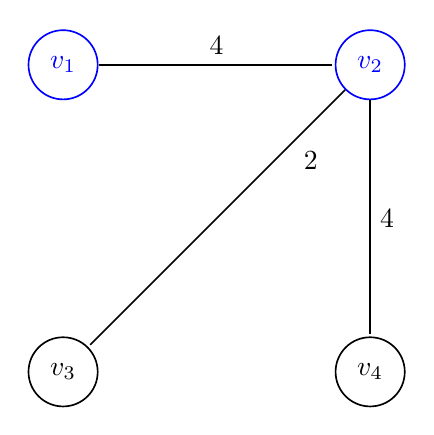
\begin{tikzpicture}[
    > = , % arrow head style
    shorten > = 1pt, % don't touch arrow head to node
    auto,
    node distance = 3cm, % distance between nodes
    semithick % line style
    ]

    \tikzset{every state}=[
    draw = black,
    thick,
    fill = white,
    minimum size = 1mm
    ]
    \node[state,blue] (v1) {$v_1$};
    \node[state,blue] (v2) [right=of v1] {$v_2$};
    \node[state] (v3) [below =of v1] {$v_3$};
    \node[state] (v4) [below =of v2] {$v_4$};
  
    \path[->] (v1) edge[]  node[]{4}(v2);
    \path[->] (v2) edge[]  node[pos=0.2,below right]{2} (v3);
    \path[->] (v2) edge  node[]{4}(v4);
\end{tikzpicture}\\\\
Since not all vertices have been visited, the algorithm recursively calls itself on the unvisited neighbors of $v_2$, which in this case are $v_3$ and $v_4$. Assuming that $v_3$ is visited before $v_4$, $v_3$ is marked as visited and added to $S$. Therefore $S= v_1, v_2, v_3$.
\\\\
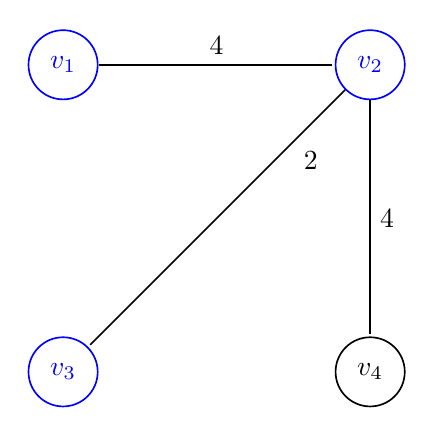
\begin{tikzpicture}[
    > = , % arrow head style
    shorten > = 1pt, % don't touch arrow head to node
    auto,
    node distance = 3cm, % distance between nodes
    semithick % line style
    ]

    \tikzset{every state}=[
    draw = black,
    thick,
    fill = white,
    minimum size = 1mm
    ]
    \node[state,blue] (v1) {$v_1$};
    \node[state,blue] (v2) [right=of v1] {$v_2$};
    \node[state,blue] (v3) [below =of v1] {$v_3$};
    \node[state] (v4) [below =of v2] {$v_4$};
  
    \path[->] (v1) edge[]  node[]{4}(v2);
    \path[->] (v2) edge[]  node[pos=0.2,below right]{2} (v3);
    \path[->] (v2) edge  node[]{4}(v4);
\end{tikzpicture}\\\\
Since not all vertices have been visited, and $v_3$ has no neighbors, the algorithm now visits another neighbor of $v_2$ which in this case is $v_4$. Hence $v_4$ is marked as visited and added to $S$. Therefore $S= v_1, v_2, v_3, v_4$.
\\\\
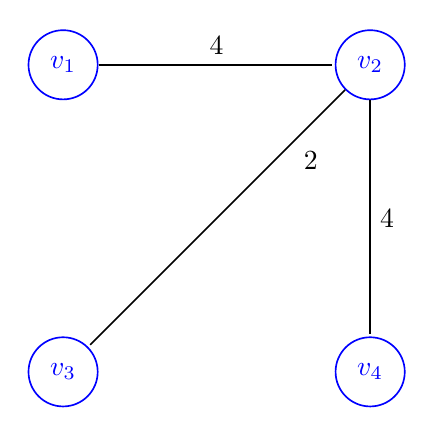
\begin{tikzpicture}[
    > = , % arrow head style
    shorten > = 1pt, % don't touch arrow head to node
    auto,
    node distance = 3cm, % distance between nodes
    semithick % line style
    ]

    \tikzset{every state}=[
    draw = black,
    thick,
    fill = white,
    minimum size = 1mm
    ]
    \node[state,blue] (v1) {$v_1$};
    \node[state,blue] (v2) [right=of v1] {$v_2$};
    \node[state,blue] (v3) [below =of v1] {$v_3$};
    \node[state,blue] (v4) [below =of v2] {$v_4$};
  
    \path[->] (v1) edge[]  node[]{4}(v2);
    \path[->] (v2) edge[]  node[pos=0.2,below right]{2} (v3);
    \path[->] (v2) edge  node[]{4}(v4);
\end{tikzpicture}\\\\
Since all vertices have been visited, the TAMSA adds $v_1$ to $S$ and returns it. Hence the TAMSA returns the Hamiltonian cycle $v_1, v_2, v_3, v_4, v_1$ of weight 23.
\end{example}
From Example \ref{tamsa_demonstration} and Example \ref{example_nna_explanation} one can observe that the NNA and the TAMSA returned the same Hamiltonian cycle. Also similarly to the NNA, the TAMSA returns bad approximations for the graph presented in Example \ref{nna_fail}. This is true because of the following. Suppose that $G(V,E,f)$ is the graph in Example \ref{nna_fail}, and $v_1$ is the vertex chosen randomly by the TAMSA in bullet point number one of the TAMSA pseudo code, when given $G$ as input. The minimum weight spanning tree of $G$ is the same as the minimum weight spanning tree of the graph $G^\prime$ in Example \ref{example4}. This is true because, $G$ and $G^\prime$ differ only in the weight of the edge $\{v_3, v_4\}$, were this edge is not included in the minimum weight spanning tree of $G^\prime$. Hence, if $f(\{v_3, v_4\})$ is very large (greater than 10), and the other edges weights remain the same, the edge $\{v_3, v_4\}$ will not be included in the minimum weight spanning tree of $G$ and hence, other edges will be used (which are identical to those of $G^\prime$). Since the minimum weight spanning tree of $G$ is the same as that of $G^\prime$, then by Example \ref{example_prim}, the TAMSA will return the Hamiltonian cycle $ H = v_1, v_2, v_3, v_4, v_1$ when given $G$ as input. Now, since $f(\{v_3, v_4\})$ is very large and $\{v_3, v_4\}$ is an edge in H, the weight of $H$ would be very large. As a result, the weight of $H$ would differ a lot from the optimal solution. Note that, this problem would not happen if the preorder traversal is started from vertex $v_4$. In fact, the Hamiltonian cycle returned by the TAMSA would be $H = v_4, v_2, v_3, v_1, v_4$ (assuming $v_3$ is visited before $v_1$ when considering $v_2$), where the edge $\{v_3, v_4\}$ of weight $M$ is not in $H$. Therefore, from this paragraph it can be concluded that the quality of the approximation returned by the TAMSA depends on the starting vertex of the preorder walk.\\\\
Consider the TSP as defined in Definition \ref{TSP}. Similarly to the NNA, the approximation ratio of the TAMSA when applied to the TSP is unknown. In addition to this, Theorem \ref{no_approx_tsp}, guarantees that the TAMSA is not a constant approximation algorithm for the TSP, unless P=NP. Therefore, since it is not known whether P=NP, it is not known if the TAMSA is a constant approximation algorithm for the TSP. However, what is known is that the TAMSA is a 2-approximation algorithm for the Metric-TSP \cite{cormen_leiserson_rivest_stein}. This fact is proved in Theorem \ref{2_approx} below. Before proving Theorem \ref{2_approx}, the concept of a full walk will be explained because, it is going to be used in the proof.\\\\
Consider the preorder tree walk algorithm description provided in this section. Let $S$ be an arbitrary Hamiltonian cycle returned by the preorder tree walk algorithm. Suppose that, the preorder tree walk algorithm is currently at a vertex $u$. According to the preorder tree walk algorithm description, the algorithm first marks $u$ as visited, adds $u$ to $S$, and then it recursively calls itself on all the unvisited neighbors $v_1, ..., v_k$ of $u$. From the preorder tree walk algorithm description it can be deduced that, the algorithm returns to $u$ when all unvisited vertices in the subgraph connected to the vertex $v_i$ for all $i$ $\in$ [$k$], are visited. In a preorder tree walk, when returning back to a vertex $v$, $v$ is not added again to $S$. To the contrary, in a full walk, when returning to a vertex $v$, $v$ is added again to $S$. Therefore, a full walk of a tree adds every vertex $v$ to $S$ whenever $v$ is first visited, and when $v$ is returned to after visiting one of the subgraphs connected to $v$ \cite{cormen_leiserson_rivest_stein}. In other words, a full walk is a preorder tree walk which lists a vertex every time it is visited. For example, a full walk of the tree in Figure \ref{tree_example} of this section would result into the walk, $v_1, v_2, v_3, v_2, v_4, v_2, v_1, v_5, v_1, v_9, v_6, v_9, v_7, v_9, v_8, v_9, v_1$. Note that in a full walk, each edge is traversed exactly twice. This is true because, at each vertex $v$, the algorithm uses an edge $e$ to traverse to a neighbor $w$ of $v$, and uses the same edge $e$ when returning back to the vertex $v$, after all the unvisited vertices in the subgraph connected to $w$ are visited. Having described what a full walk is, it is now time to prove that the TAMSA is a 2-approximation algorithm when applied to the Metric-TSP. Note that the proof for Theorem \ref{2_approx} below was adapted using ideas from \cite{cormen_leiserson_rivest_stein}.
\begin{theorem}
\label{2_approx}
The TAMSA is a 2-approximation algorithm for the Metric-TSP {\normalfont{\cite{cormen_leiserson_rivest_stein}}}.
\end{theorem}
\begin{proof}
Let $G(V,E,f)$ be an instance of the Metric-TSP, and $H^\star$ be a minimum weight Hamiltonian cycle of $G$. A spanning tree $T^\star$ can be obtained from $H^\star$ by deleting an edge from $H^\star$. This is true because, when deleting an edge from $H^\star$, no vertices of $G$ are deleted, hence, all vertices in $V$ would still be in $T^\star$. In addition to this, $T^\star$ has no cycles because, it contains less edges than vertices. As a result, by Definition \ref{spanning tree}, $T^\star$ is a spanning tree. Now, since every edge weight is positive, deleting an edge from a Hamiltonian cycle would result into a spanning tree of weight less than that of the Hamiltonian cycle. Furthermore, the weight of any spanning tree is greater than the weight of the minimum weight spanning tree. Hence, the weight of the minimum weight spanning tree gives a lower bound on the weight of the minimum weight Hamiltonian cycle. Therefore, letting $T$ be the minimum weight spanning tree of $G$, the following inequality holds:
\begin{equation}
\begin{split}
    \label{eq:1}
    f(T) \leq f(T^\star) \leq f(H^\star)\\
    \implies f(T) \leq f(H^\star)
 \end{split}
 \end{equation}
Now, let $W$ be a full walk of $T$. It was argued in this section that, a full walk of a tree $T^\prime$ uses an edge of $T^\prime$ exactly twice. Hence,
\begin{equation}
\begin{split}
    \label{eq:2}
    f(W) = 2f(T) \leq 2f(H^\star) \text{ (By Equation \ref{eq:1})}\\
    \implies f(W) \leq 2f(H^\star)
 \end{split}
 \end{equation}
However, $W$ is not a Hamiltonian cycle because it contains repetition of vertices. Now, since $G$ satisfies the triangle inequality, a path $P = u, v$ in $G$, has less weight than a path $P^\prime = u, c, v$ in $G$, $u, c, v$ $\in$ $V$. This means that, since a full walk returns to a vertex $u$ from a vertex $c$ and traverses to a vertex $v$, the full walk has a larger weight than that of traversing directly from $c$ to $v$ in $G$. Hence, by removing repetition of vertices in $W$, a sequence of vertices $H$ with the following properties is obtained. The first property is that $H$ is a Hamiltonian cycle. This is true because, $H$ contains every vertex exactly once (excluding the starting vertex of the cycle). The second property is that $H$ has a smaller weight than $W$. This is true because of the triangle inequality implications described in this paragraph. Due to the second property, the inequality below is satisfied.
\begin{equation}
\begin{split}
   \label{eq:3}
    f(H) \leq f(W)
 \end{split}
 \end{equation}
As described in this section, the difference between a full walk and a preorder walk is that in a preorder walk, vertices are not listed again when they are returned to. Hence, a preorder walk on a tree $T^\prime$ is equivalent to performing a full walk on a tree $T^\prime$ and deleting the repetition of vertices. This means that $H$ is the output of the preorder tree walk algorithm when given $T$ as input. Hence, $H$ is the Hamiltonian cycle outputted by the TAMSA. Therefore, from Equation \ref{eq:3} and Equation \ref{eq:2} it can be concluded that,
\begin{equation}
\begin{split}
   \label{eq:4}
    f(H) \leq f(W) \text{ (By Equation \ref{eq:3})}\\
    \implies f(H) \leq 2f(H^\star) \text{ (By Equation \ref{eq:2})}
 \end{split}
 \end{equation}
Hence, from Equation \ref{eq:4} it can be concluded that, the value of the approximate solution returned by the TAMSA is within a constant factor of 2 of the optimal value. Hence, the TAMSA is a 2-approximation algorithm for the Metric-TSP.
\end{proof}
Therefore, Theorem \ref{2_approx} guarantees that, the value of the approximation returned by the TAMSA when applied to the Metric-TSP, is never more than twice the optimal value, even for very large instance sizes. Recall that, this was not the case for the NNA. In fact, in Section 2.1 it was shown that, the approximation ratio for the NNA when applied to the Metric-TSP increases logarithmically with respect to the input size. That being said, it is stated in \cite{cormen_leiserson_rivest_stein} that although the TAMSA has a constant approximation ratio, it is not the best practical choice for the Metric-TSP. In fact, Christofides gave a 3/2-approximation algorithm for the Metric-TSP. However, this will not be discussed in this project because, Christofides' algorithm requires presenting mathematical concepts which are out of the scope of this project. Such mathematical concepts are those of a minimum weight perfect matching.\\\\
In Section 2.1.1 and Section 2.1.2, the aim was to present algorithms that approximate the TSP, and rigorously prove their approximation ratios when applied to a special case of the TSP (Metric-TSP). Although having approximation guarantees is important (via the approximation ratio), it is better in practice in terms of accuracy of approximations to design an algorithm that is guaranteed to find an optimal solution if given enough time. Note that this statement will be justified when comparing the algorithm's performance in Chapter 3. In the following section, two classes of algorithms called the heuristics and metaheuristics will be defined. Afterwards, an example of a metaheuristic called the Ant Colony Optimization metaheuristic is going to be defined. After doing so, an example of an Ant Colony Optimization metaheuristic called the Ant Colony System will be given. After defining the Ant Colony System, the main aim is to prove that if given enough time, the Ant Colony System applied to an arbitrary TSP instance $G$ will converge to the optimal solution of $G$ (note that the time may be arbitrarily large).
\subsubsection{The Ant Colony Optimization Algorithm}
\label{section_ACO}
To understand the nature of the Ant Colony Optimization Algorithm better, it is important to define two classes of algorithms. One important class of algorithms is that of heuristics. Heuristics are algorithms that seek to obtain near-optimal solutions to a problem in a short time (polynomial), without guaranteeing that an optimal solution will be found \cite{dorigo_stutzle_thomas_2004}. From what has been discussed so far, one can deduce that the TAMSA and the NNA are heuristic algorithms because, they both try to obtain near-optimal solutions to the TSP, without guaranteeing that the returned solution is an optimal one. The other important class of algorithms is that of metaheuristics.  A metaheuristic is a set of algorithmic notions that can be used to define heuristic methods for a wide variety of problems \cite{dorigo_stutzle_thomas_2004}. In other words this means that, a metaheuristic algorithm is a general framework that can be used to define different heuristics which may not solve the same problem. Note that a metaheuristic is different than a heuristic because, heuristic algorithms are specifically written to solve only one problem. For example, the NNA and the TAMSA can only approximate the TSP. Some examples of metaheuristic algorithms are Tabu Search, Simulated Annealing, Evolutionary Computing, and the ACO algorithm \cite{dorigo_stutzle_thomas_2004}. Note that for convenience, the terms `metaheuristic algorithm' and `algorithm' are used interchangeably.\\\\
The ACO algorithm is a metaheuristic algorithm which was inspired from the behavior of ants in real ant colonies. Ants are capable of finding the shortest path from a food source to their nest and vice-versa without using any visual signals. Although ants do not use visual cues, it does not mean that they cannot communicate. In fact, ants deposit a chemical known as pheromone when they walk, and they probabilistically prefer to move into directions which are rich in pheromone. The trail of pheromone left behind by an ant while walking is called a pheromone trail. It is important to note that an ant may still move to a direction which is not rich in pheromone, however, the probability of doing so is very small. The movement of ants in directions which are not rich in pheromone is important in real ant colonies because, it helps ants explore other ways of constructing a path from a food source to the nest which may result into a shorter path. \cite{dorigo_gambardella_1997}, \cite{dorigo_stutzle_thomas_2004}\\\\ 
The reason why ants are able to find short paths from a food source to their nest is because, pheromone accumulates quicker on shorter paths. Pheromone accumulates quicker on shorter paths because of the following. Suppose that ants start to wander randomly to different directions in their environment starting from a food source. Obviously, ants that choose shorter paths to their nest will arrive much quicker than the ants that choose longer paths. This means that, on the way back to the food source, the ants that used the shorter paths will smell more pheromone on the shorter paths than on the longer paths because, the ants that choose the longer paths would have still not arrived at their nest (the pheromone trail is not yet constructed). In addition to this, pheromone evaporates gradually over time. Hence, the longer a path $P$ is, the more pheromone evaporation $P$ experiences until the ants using $P$ reach their destination. As a result, the ants would probabilistically prefer to move back to the food source using the shorter paths because they simply would contain more pheromone. Over time this would result into higher accumulation of pheromone on a shortest path, which would make the majority of the ants to choose a shortest path in order to travel from their nest to a food source and vice-versa. \cite{dorigo_gambardella_1997}, \cite{dorigo_stutzle_thomas_2004}\\\\
What follows is an example that demonstrates at an abstract level how the ACO metaheuristic can be applied to the Shortest Path Problem defined in Example \ref{example decision/optimization}.
\begin{example}
\label{explain_ACO}
\normalfont{Suppose} that the shortest path from vertex $v_1$ to vertex $v_4$ of the graph $G$ below must be found.\\\\
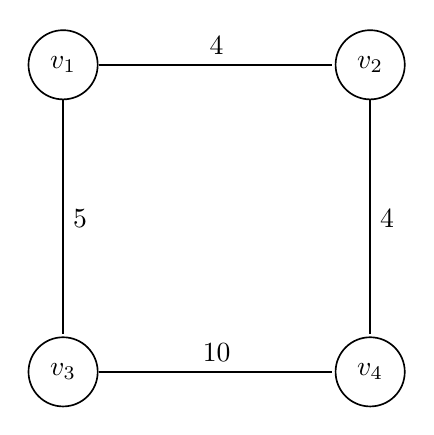
\begin{tikzpicture}[
    > = , % arrow head style
    shorten > = 1pt, % don't touch arrow head to node
    auto,
    node distance = 3cm, % distance between nodes
    semithick % line style
    ]

    \tikzset{every state}=[
    draw = black,
    thick,
    fill = white,
    minimum size = 1mm
    ]
    \node[state] (v1) {$v_1$};
    \node[state] (v2) [right=of v1] {$v_2$};
    \node[state] (v3) [below =of v1] {$v_3$};
    \node[state] (v4) [below =of v2] {$v_4$};
  
    \path[->] (v1) edge[]  node[]{4}(v2);
    \path[->] (v1) edge  node[]{5}(v3);
    \path[->] (v3) edge  node[]{10}(v4);
    \path[->] (v2) edge  node[]{4}(v4);
\end{tikzpicture}
\\\\
Clearly, the ACO framework can be applied to the Shortest Path Problem on $G$ by letting the ant's environment be $G$, and the food source and the nest be $v_1$ and $v_4$ respectively. The ants would then find the shortest path due to the following. Since no ant has yet started to walk in it's environment, no pheromone has yet been deposited. Hence, for every ant starting at vertex $v_1$, $v_2$ and $v_3$ have the same probability of being chosen because no pheromone is yet deposited on the edges $\{v_1, v_2\}$, $\{v_1, v_3\}$. Hence, assuming that all ants at $v_1$ move at the same time, half of the ants probabilistically choose to move to $v_2$ and half of the ants probabilistically choose to move to $v_3$.\\\\
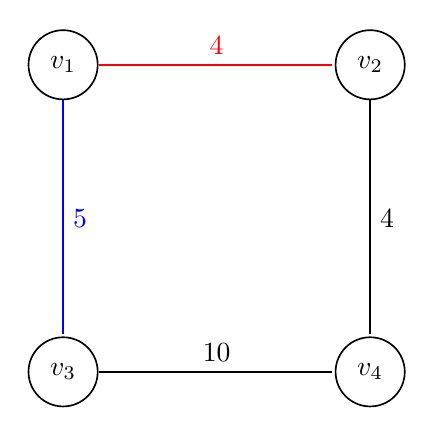
\begin{tikzpicture}[
    > = , % arrow head style
    shorten > = 1pt, % don't touch arrow head to node
    auto,
    node distance = 3cm, % distance between nodes
    semithick % line style
    ]

    \tikzset{every state}=[
    draw = black,
    thick,
    fill = white,
    minimum size = 1mm
    ]
    \node[state] (v1) {$v_1$};
    \node[state] (v2) [right=of v1] {$v_2$};
    \node[state] (v3) [below =of v1] {$v_3$};
    \node[state] (v4) [below =of v2] {$v_4$};
  
    \path[->] (v1) edge[red]  node[]{4}(v2);
    \path[->] (v1) edge[blue]  node[]{5}(v3);
    \path[->] (v3) edge  node[]{10}(v4);
    \path[->] (v2) edge  node[]{4}(v4);
\end{tikzpicture}
\\\\
Suppose that a constraint is added such that each ant does not visit vertices that it has already visited. This can be easily done by assigning a list of vertices to each ant $k$ which contains the vertices that ant $k$ has already visited. As a result, the ants at $v_3$ and $v_2$ have only one vertex to move to because $v_1$ has already been visited. Therefore, all ants from $v_2$ and $v_3$ move to vertex $v_4$.\\\\
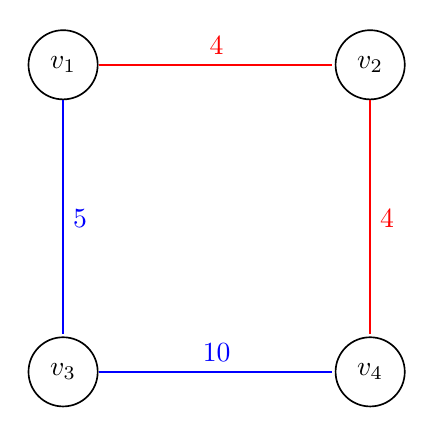
\begin{tikzpicture}[
    > = , % arrow head style
    shorten > = 1pt, % don't touch arrow head to node
    auto,
    node distance = 3cm, % distance between nodes
    semithick % line style
    ]

    \tikzset{every state}=[
    draw = black,
    thick,
    fill = white,
    minimum size = 1mm
    ]
    \node[state] (v1) {$v_1$};
    \node[state] (v2) [right=of v1] {$v_2$};
    \node[state] (v3) [below =of v1] {$v_3$};
    \node[state] (v4) [below =of v2] {$v_4$};
  
    \path[->] (v1) edge[red]  node[]{4}(v2);
    \path[->] (v1) edge[blue]  node[]{5}(v3);
    \path[->] (v3) edge[blue]  node[]{10}(v4);
    \path[->] (v2) edge[red]  node[]{4}(v4);
\end{tikzpicture}
\\\\
Now, since the red path is shorter than the blue path, the ants following the red path arrive at vertex $v_4$ before the ants following the blue path. Hence, on the way back to vertex $v_1$, the red path has more pheromone than the blue path because, more pheromone is evaporated on the longer path until all ants arrive at $v_4$. Therefore, the majority of the ants at $v_4$ would probabilistically choose to travel to $v_1$ using the red path. As a result, the red path keeps on accumulating more pheromone than the blue path and eventually this would lead to a situation were almost all ants would choose the red path when traveling from $v_1$ to $v_4$ and vice-versa. To conclude, the ACO algorithm for the Shortest Path Problem given $(G, v_1, v_4)$ as instance can then return the best found path $P$ (in this case the red path) when either the majority of the ants are traveling through $P$, or, it can return $P$ after a maximum number of iterations are reached.  
\end{example}
Having described the basic ideas behind the ACO metaheuristic, it is now time to describe the requirements the algorithm which implements the ACO framework must follow, in order to be successfully applied to the TSP. Let $G(V,E,f)$ be an instance of the TSP. As described in Example \ref{explain_ACO}, the ant's environment can be represented by $G$. In addition to this, since the goal of the TSP is to find a minimum weight Hamiltonian cycle, it does not matter which vertex represents the food source and which vertex represents the nest, because, all vertices have to be visited. What is important is that when an ant starts traversing vertices in a graph, it doesn't move to vertices that it has already visited. This can be done as discussed in Example \ref{explain_ACO} above, by giving each ant a list of vertices called  the working memory, which is used to remember which vertices it has already visited. Note that although real ants do not posses a working memory, the working memory is vital for the artificial ants to compute a Hamiltonian cycle, otherwise, ants may produce walks of $G$ with repetition of vertices. Another important thing is that the artificial ants must keep the order of how the vertices are visited. This can be easily done by always adding a new vertex that an ant visits at the end of the working memory. In what follows, a specific type of ACO metaheuristic will be discussed in detail with specific reference to how it can be applied to the TSP. This metaheuristic algorithm is called the Ant Colony System (ACS) in literature. \cite{dorigo_gambardella_1997}, \cite{dorigo_stutzle_thomas_2004}\\\\
The ACS for the TSP can be described as follows. Suppose that $G(V,E,f)$ is a TSP instance. At the start of the algorithm, each ant is placed on a random vertex of $G$. At each time step, every ant $k$ is moved to a vertex of $G$ which is not in the working memory of ant $k$, and this is repeated until all vertices of $G$ are in the working memory of ant $k$. The new vertex that each ant must move to is determined using a probabilistic function. As discussed so far in this subsection, the ants must probabilistically prefer to move in directions with high pheromone. Hence, at each time step, the probabilistic function must be in such a way that every ant should probabilistically prefer to choose vertices, which are connected via edges to the vertex the ant is currently on with high pheromone. However, since the TSP is based on finding shorter connections, then the length of the edges must also effect the direction the ants must move to. Therefore, the probabilistic function must be a function of both the pheromone accumulated on the edges, and of the length of the edges connecting the current vertex the ant is on with a candidate vertex, where, the higher the weight of an edge $e$  is, the less chance $e$ has of being chosen by an ant. Due to this probabilistic function, ants would probabilistically prefer to move to vertices that are connected by edges with high pheromone and which are close-by. \cite{dorigo_gambardella_1997}, \cite{dorigo_stutzle_thomas_2004}\\\\
Another important component of the ACS is local trail updating. Local trail updating is the reduction of pheromone on the edges chosen by an ant at each time step. The aim of local trail updating is to reduce the pheromone of an edge $e$, after it is chosen by an ant so that $e$ is less desirable for other ants. Local trail updating is important because, it increases the probability that ants explore other edges that were not visited by any other ant, and hence, lowers the probability that the ants generate the same sub-optimal solution repeatedly. It is important to note that, local trail updating was inspired from pheromone evaporation in real ant colonies. In what has been discussed so far, it was argued that pheromone accumulates quicker on shorter paths in real ant colonies. The ACS encourages this behavior by making the ants that produce the shorter Hamiltonian cycles deposit more pheromone on the edges constituting their Hamiltonian cycle at every iteration. As a result, there would be more pheromone present on edges that constitute the shorter Hamiltonian cycles. This procedure is called global trail updating. One way to go about global trail updating is to make the ant that produces the best Hamiltonian cycle since the first iteration of the algorithm add more pheromone on the edges constituting it's Hamiltonian cycle. Another way is to make the ant that produces the iteration's best Hamiltonian cycle deposit more pheromone on the edges constituting it's Hamiltonian cycle. According to \cite{dorigo_stutzle_thomas_2004}, the former is better than the latter empirically. Hence, in what remains, global trail updating is performed by the ant that produces the Hamiltonian cycle of minimum weight since the first iteration of the ACS (global best solution). Note that the ant that produces the global best solution is called the global best ant. \cite{dorigo_gambardella_1997}, \cite{dorigo_stutzle_thomas_2004} \\\\
It is important to note that there are different ACO algorithms that could have been applied to the TSP. The ACS was chosen because, it is one of the most empirically successful ACO algorithms in terms of accuracy of approximations \cite{dorigo_stutzle_thomas_2004}. It is important to note that later on in this section, other ACO algorithms will be briefly described by discussing how they vary from the ACS. The discussion will now proceed by presenting the pseudocode of an algorithm (Algorithm \ref{ACO_ALG}) for the TSP that implements the ACS framework. In Algorithm \ref{ACO_ALG} below, $G(V,E,f)$ is an instance of the TSP, and $g$ is a probabilistic function with the properties described in the previous paragraphs. Also, $a.current\_vertex$ is the variable containing the vertex that ant $a$ is currently on. Note that Algorithm \ref{ACO_ALG} was constructed using ideas from \cite{dorigo_gambardella_1997}.
\begin{algorithm}[H]
\begin{algorithmic}[1]
\State $best\_ham\_cycle$ = ()
\State $best\_ham\_cycle.weight$ = $\infty$
\While{(!finished)}
          \State Place $m$ new ants on $m$ randomly selected vertices in $V$.
          \While{not all ants have completed a Hamiltonian cycle of $G$}
		\For {every ant $a$}
			\State move $a$ to vertex $v$ $\in$ $V$ chosen using the probabilistic function $g$.
			\State Perform local trail updating on the edge $\{a.current\_vertex, v\}$
		\EndFor
	\EndWhile
	\State $A$ = ant which produces a minimum weight Hamiltonian cycle of this iteration.
	\If{$best\_ham\_cycle.weight$ $\geq$ $A.Hamiltonian\_Cycle.weight$}
		\State $best\_ham\_cycle$ = $A.Hamiltonian\_Cycle$
	\EndIf
           \State Perform global pheromone update on the edges of $G$ constituting the Hamiltonian cycle $best\_ham\_cycle$
\EndWhile
\State Return $best\_ham\_cycle$
\caption{: ACS\_TSP($G(V,E,f)$)}
\label{ACO_ALG}
\end{algorithmic}
\end{algorithm}
For Algorithm \ref{ACO_ALG} to be implemented, there remains to define the probabilistic function $g$, the global trail updating formula, and the local trail updating formula. As stated in \cite{dorigo_gambardella_1997}, there are different ways how the probabilistic function and the global/local trail updating formulas can be defined. However, the ones suggested by Dorigo and Gambardella in \cite{dorigo_gambardella_1997} will be presented. Note that the probabilistic function, and the local/global trail updating formula will be presented in their general form (i.e. for the ACS applied to any problem). While presenting these formulas, it will be discussed how they can be applied to the TSP. Note that from this point onward, any definitions and terms that will be defined will be used throughout the entire section. \\\\Let $G(V,E,f)$ be an instance of the TSP. An ant $k$ on vertex $r$ chooses the vertex $s$ to move to among those vertices which do not belong to its working memory $M_k$, by applying the probabilistic formula below.
\begin{equation}
  \label{eq:aco1}
  s=\begin{cases}
            \displaystyle{\argmax\limits_{u \notin M_k} \left\{[\tau(\{r,u\})].\left[\eta(\{r, u\})\right]^\beta \right\}} &\text{   if $q$ $\leq$ $q_0$}\\ 
             S &\text{ 	otherwise}
            \end{cases}
\end{equation}
where $\tau(\{r,u\})$ is the amount of pheromone on the edge $\{r,u\}$, $\eta(\{r,u\})$ is a problem specific function where for the TSP it was chosen to be the inverse of the weight of the edge $\{r,u\}$, $\beta$ is a parameter which weighs the importance of the pheromone level of an edge $\{r,u\}$ and the closeness of $u$ to $r$, 0 $\leq$ $q$ $\leq$ 1 is a random value chosen with uniform probability, 0 $\leq$ $q_0$ $\leq$ 1 is another parameter, and $S$ is a random variable which is selected according to the following probability distribution:
\begin{equation}
  \label{eq:aco2}
  p_k(\{r,s\})=\begin{cases}
             \displaystyle {\frac{[\tau(\{r,s\})].[\eta(\{r, s\})]^\beta}{\sum_{u \notin M_k} [\tau(\{r,u\})].[\eta(\{r, u\})]^\beta }} &\text{ if $s$ $\notin$ $M_k$}\\ 
             0 &\text{ 	otherwise}
            \end{cases}
\end{equation}
where $p_k(r,s)$ is the probability of ant $k$ on vertex $r$ to choose vertex $s$. \cite{dorigo_gambardella_1997}\\\\
The idea behind Formula \ref{eq:aco1} is the following. When an ant $k$ wants to move to a new vertex, it picks a random number $q$ in the interval [0,1], where each number in this interval has equal probability of being chosen. Then, if $q$ $\leq$ $q_0$, since $\eta$ was chosen to be the inverse of the weight of an edge, the edge with the largest amount of pheromone per edge weight is chosen. It is important to note that, the larger the amount of pheromone on an edge is, the more chance an edge has to be the maximum element in the argument list of Formula \ref{eq:aco1}. In addition to this, the smaller the weight of an edge is, the larger the value of $[\tau(\{r,u\})].\left[\eta(\{r, u\})\right]^\beta$ is. Therefore, it can be concluded that the case $q$ $\leq$ $q_0$ makes an ant choose the edge with the largest amount of pheromone per edge weight. In other words, the case $q$ $\leq$ $q_0$ forces an ant to choose the edge which has been chosen by the majority of ants as required by the ACO metaheuristic. \cite{dorigo_gambardella_1997}, \cite{dorigo_stutzle_thomas_2004}\\\\
When $q$ is less than $q_0$, the ant randomly picks a vertex with probability defined by the probability distribution in Formula \ref{eq:aco2} above. The idea behind Formula \ref{eq:aco2} above is the following. If a vertex is already in the working memory of an ant, then it has no chance of being selected. Hence, it's probability is zero. This will ensure that ants will not produce a walk with repetition of vertices. If a vertex $s$ is not in the working memory of an ant $k$, the probability of ant $k$ on vertex $r$ to choose $s$ depends on the amount of pheromone on the edge $\{r,s\}$ per edge weight of $\{r,s\}$, where, the larger this ratio is, the larger the probability of the vertex $s$ is to being chosen. Therefore, this equation makes an ant probabilistically prefer edges with large pheromone and small weight. However, unlike the case $q$ $\leq$ $q_0$ in Equation \ref{eq:aco1}, this does not mean that a vertex with a small probability cannot be chosen. This mimics the case when real ants move to directions which are not rich in pheromone. As discussed earlier, this is necessary in real ant colonies because it may help ants to find shorter paths from a food source to their nest. Similarly, the movement of artificial ants (ants in the ACO algorithm) to vertices with low probability defined by Formula \ref{eq:aco2}, may help the algorithm find Hamiltonian cycles of lesser weight. \cite{dorigo_gambardella_1997}, \cite{dorigo_stutzle_thomas_2004}\\\\
Therefore, from the above two paragraphs it can be concluded that, an ant can either move to new vertices using experience gathered from previous ants with probability $q_0$ (using the largest amount of pheromone per edge weight), or it can perform a biased exploration towards edges of small weight but with high pheromone levels with probability $(1-q_0)$. As a result, the value of $q_0$ determines the amount of exploration that will be performed by the ACS. According to  \cite{dorigo_gambardella_1997}, the best value of $q_0$ was empirically found to be 0.9. From this observation one can deduce that, it is more important for the ACS to gather information from previous ants than exploring other edges in the TSP instance. \cite{dorigo_gambardella_1997}, \cite{dorigo_stutzle_thomas_2004}\\\\
The next formula that needs to be presented is the global trail updating formula. As discussed previously, the idea behind global trail updating is to reward edges which belong to shorter Hamiltonian cycles, with more pheromone. It was also discussed that this will be achieved by forcing the global best ant to add more pheromone on the edges that belong to it's Hamiltonian cycle. The global trail updating formula can be seen in Formula \ref{eq:aco3} below, and it is the one presented in \cite{dorigo_stutzle_thomas_2004}. Therefore, the global best ant performs global trail updating on every edge $\{r,s\}$ forming part of it's solution using the formula below:
\begin{equation}
  \label{eq:aco3}
  \tau(\{r,s\})=(1-p).\tau(\{r,s\})+ p.\Delta\tau(\{r,s\})
\end{equation}
where $\tau(\{r,s\})$ is the amount of pheromone on edge $\{r,s\}$, $p$ is the evaporation rate which mimics evaporation of pheromone in real ant colonies, and $\Delta\tau(\{r,s\})$ is a problem specific value which for the TSP is chosen to be, the inverse of the weight of the best Hamiltonian cycle produced by the global best ant.\\\\
From Formula \ref{eq:aco3} it can be deduced that, the shorter a Hamiltonian cycle belonging to the global best ant is, the larger is $\Delta\tau(\{r,s\})$ and hence, more pheromone is added to it's edges. As a result, this will accumulate more pheromone on the edges belonging to shorter Hamiltonian cycles and thus make shorter Hamiltonian cycles more desirable for other ants. As already remarked, although it is desirable to have a lot of pheromone on the edges that form part of short Hamiltonian cycles, the ACS must not create a situation where an edge is always chosen by all ants. Otherwise, as previously discussed, the ants may not find shorter Hamiltonian cycles. As it can be seen in Formula \ref{eq:aco3}, this problem is solved by reducing some of the added pheromone by the aid of the evaporation rate $p$. As a result, $p$ is typically a value in the interval (0,1]. In fact, Dorigo and Gambardella \cite{dorigo_gambardella_1997} found out empirically that, the best value of $p$ is 0.1. \cite{dorigo_gambardella_1997}\\\\
For Algorithm \ref{ACO_ALG} to be implemented, there remains to present the local trail updating formula. The local trail updating formula that will be presented is the one suggested in \cite{dorigo_stutzle_thomas_2004}. Therefore, when an ant on vertex $r$ chooses vertex $s$ it modifies the pheromone on the edge $\{r,s\}$ using the local trail updating formula below.
\begin{equation}
  \label{eq:aco4}
  \tau(\{r,s\})=(1-\zeta).\tau(\{r,s\})+\zeta.\tau_0
\end{equation}
where $\tau_0$ is the value representing the amount of pheromone deposited on an edge when it is chosen by an ant, $\tau(\{r,s\})$ is the amount of pheromone on edge $\{r,s\}$, and 0 $<$ $\zeta$ $<$ 1 is the evaporation rate. It is important to note that $\tau_0$ and $\zeta$ are usually chosen in such a way that after the local trail updating formula is applied, the pheromone on the chosen edge is reduced. This is important because as discussed before, the aim of local trail updating is to avoid having all ants choosing the same edges. As a result, an experimentally good value for $\zeta$ was found to be 0.1, and an experimentally good value for $\tau_0$ was experimentally found to be $\displaystyle{\frac{1}{nC^{nn}}}$ where $n$ is the number of vertices in the TSP instance, and $C^{nn}$ is the length of the Hamiltonian cycle returned by the NNA. It is important to note that normally, the pheromone values of the edges at the start of the algorithm are initialized to the value of $\tau_0$. Another observation is that although $\zeta$ and $p$ both represent the evaporation rate, their values can be different. \cite{dorigo_gambardella_1997}, \cite{dorigo_stutzle_thomas_2004}\\\\
As already remarked, the ACO algorithm that was applied to the TSP in this section was the ACS. However, there are other ACO algorithms that could have been applied to the TSP. Two of these ACO algorithms are the Ant System (AS) and the Elitist Ant System (EAS). The main difference between the ACS, AS and EAS is how the pheromones on the edges are updated from one iteration to the next. For example in the AS, no pheromone update is carried out until all ants compute a solution of the problem they are applied to. In addition to this, after all ants compute their solution, every edge in the graph gets it's pheromone reduced. After all edges get their pheromone reduced, all ants add more pheromone on the edges they used. One can observe that this differs a lot from the ACS because, the AS performs pheromone evaporation on all edges in the graph. In addition to this, unlike the ACS, the AS does not perform global trail updating. The other ACO algorithm variant that was mentioned in this paragraph is the EAS. The EAS is an extension of the AS, where the only difference is that at each iteration, the global best ant adds more pheromone on the edges that constitute it's solution. Note that the AS and the EAS where only briefly described to show that there are other ACO algorithms that can be applied to any problem including the TSP. A detailed explanation on these ACO algorithms is given in \cite{dorigo_stutzle_thomas_2004}. \cite{dorigo_stutzle_thomas_2004}\\\\
Since ants are capable of finding a shortest path from a food source to their nest, it is now natural to ask whether the ACS is able to find a minimum weight Hamiltonian cycle if given enough time to execute. More generally, if a problem $P$ can be solved by an ACO algorithm $A$, will $A$ eventually find the optimal solution of $P$? In literature, when an optimization algorithm (algorithm for an optimization problem) $A$ finds an optimal solution for a problem, $A$ is said to converge. It is important to note that, if an ACO algorithm $A$ converges, then $A$ can find the optimal solution of every problem that it can be applied to. Unfortunately, it is not easy to determine whether the ACO metaheuristic converges because, the brief history of the ACO metaheuristic is a history of experimental research \cite{dorigo_stutzle_thomas_2004}. In addition to this, the fact that the ACO metaheuristic can be applied to a wide variety of problems, makes theoretical analysis very difficult \cite{dorigo_stutzle_thomas_2004}. Due to these reasons, all of the convergence results about the ACO metaheuristic that are known of only apply to specific variants (ex. ACS) \cite{dorigo_stutzle_thomas_2004}.\\\\
As already hinted in the previous paragraph, the theoretical property of algorithms that will be analyzed in this project is that of convergence. In general, there are at least two types of convergence in the ACO framework. These are convergence in value, and convergence in solution. An optimization algorithm converges in value if it generates the optimal solution at least once. On the other hand, an optimization algorithm converges in solution if it reaches a state which repeatedly generates the same optimal solution. It is important to note that, although convergence in solution is stronger than convergence in value, in this section only convergence in value will be considered. The reason is that, in optimization, the algorithm solving the optimization problem can be stopped once an optimal solution is found. For example, in Algorithm \ref{ACO_ALG}, once the value of best\_ham\_cycle.weight becomes equal to the optimal value, it will never change again because, the optimal value is the smallest possible value, hence, the algorithm can be stopped. In what follows, an ACO algorithm variant called $ACO_{bs, \tau_{min}}$ will be defined, and it will be shown that the $ACO_{bs, \tau_{min}}$ algorithm converges in value if given enough time. Afterwards, it will be shown that the proof of convergence of $ACO_{bs, \tau_{min}}$ applies also to the ACS. As a result, it can then be confirmed that the ACS will eventually converge to a minimum weight Hamiltonian cycle if given enough time. \cite{dorigo_stutzle_thomas_2004}\\\\
In what has been discussed so far, it has always been assumed that the ants perform walks on the instance of the optimization problem that is inputted to the ACO algorithm implemented. For example in the ACS for the TSP, the ants perform walks directly on the TSP graph instance. However, this can only be done if the instance of the problem being consider is a graph instance. Optimization problems who's instances are not a graph require their instances to be transformed into graph instances. Otherwise if not, the ACO algorithm cannot be applied on that problem. Therefore, before defining the $ACO_{bs, \tau_{min}}$ algorithm, a number of concepts must first be formalized. Note that the terms/concepts that will be defined/formalized/generalized from this point onward will be used throughout in what follows. A minimization problem $P$ can be defined as a triple $(S, f, \Omega)$ where, $S$ is the set of all candidate solutions of $P$, $f$ : S $\mapsto$ $\real^+$ is called the cost function, and $\Omega$ is a set of constraints which defines the set of feasible candidate solutions $\widetilde{S}$ $\subseteq$ $S$. As a consequence of this definition, $s^\star$ $\in$ $\widetilde{S}$ is an optimal solution of $P$ if $f(s^\star)$ $\leq$ $f(s)$ for all $s$ $\in$ $S$. In general, $P$ can be mapped to a new problem $A$ which can be characterized in terms of a graph as follows. Let $C=\{c_1, c_2, ..., c_N\}$ be a set of components/vertices, where $N$ is the size of $C$, and let $X$ be the finite set of states the algorithm solving the problem $A$ can be in, defined in terms of all possible sequences $(c_i, c_j, ..., c_h, ...)$ over the elements of $C$, such that the length of every state is finite. Denote by $n$ the maximum possible length of an element $x$ in $X$. In addition to this, let $C$ and $S$ be in such a way that $S$ $\subseteq$ $X$. Also, let $\widetilde{X}$ $\subseteq$ X be a set of states of $A$ such that, if an element $x$ is in $\widetilde{X}$, then, $x$ can be transformed into an element $s$ which satisfies $\Omega$ by adding more components to $x$. As a result, $s$ $\in$ $\widetilde{S}$. In addition to this, let $S^\star$ be the set of all optimal solutions of $A$. As a result, $S^\star$ $\subseteq$ $\widetilde{X}$ and $S^\star$ $\subseteq$ $S$. Given the definitions in this paragraph, an ACO algorithm can then be applied to $A$ such that, the ants perform walks on the graph $G_c=(C,L,\mathrm{T})$, where $L$ is the set of edges that fully connects the components in $C$, and $\mathrm{T}$ is a matrix of pheromone trails, where $\tau_{ij}$=$\mathrm{T_{ij}}$ denotes the pheromone value of the edge $\{c_i, c_j\}$ in $G_c$. It is important to note that in this case, the graph $G_c$ will not posses the property of changing with respect to time. Hence, the problems that will be considered in this section are static with respect to time (static problems for short). Therefore, the convergence proofs that will be presented later on in this section only apply to static problems. Note that the TSP is a static problem because, the graph instance does not change during an algorithm's execution. Note that, what is important to take from these formalizations is that, if a minimization problem $P$ is to be solved using an ACO algorithm, then a graph $G_c$ must be constructed for the ants to solve $P$. \cite{dorigo_stutzle_thomas_2004}\\\\
To understand better the concepts formalized in the previous paragraph, these concepts are now going to be presented in the context of the TSP. The TSP can be represented formally as an optimization problem as follows. Given a TSP instance $G(V,E,g)$, $S$ can contain tuples of vertices in $G$, where repetition of vertices in the tuples is allowed. As a result, $S$ contains all possible walks in $G$. Since in the TSP, weights of walks must be optimized, the cost function $f$ is chosen to be $g$. The set of feasible candidate solutions $\widetilde{S}$ must contain the solutions which satisfy the problem's constraints. Hence, in the context of the TSP, the solutions in $\widetilde{S}$ must form a Hamiltonian cycle. As a result, the constraints in $\Omega$ must force $\widetilde{S}$ to contain only Hamiltonian cycles. Therefore, two constraints are only needed in $\Omega$. The first constraint in $\Omega$ is that every $s$ in $\widetilde{S}$ must be of the form $(v_1, v_2, ...,v_n, v_1)$, where apart from $v_1$, no other vertex is allowed to be repeated in $s$. The second constraint in $\Omega$ is that for every $s$ in $\widetilde{S}$, $s$ must contain all the vertices in $V$. The next term that needs to be defined is $S^\star$. In the context of the TSP, $S^\star$ is the set of all minimum weight Hamiltonian cycles in $G$. Now, since the TSP's instance are graphs, the ants can directly use $G$ to perform it's walks. As a result, $G_c$ = $G$, $C = V$ and $E=L$. What remains to be defined is $X$ and $\widetilde{X}$. In the context of the TSP, $X=S$ and $\widetilde{X}$ is the set of all elements in $X$ of the form $x$ = $(v_1, v_2, ..., v_n)$, such that if more vertices are added to $x$, $x$ is transformed into a Hamiltonian cycle. Note that, what is important to take from these formalizations is that, if a minimization problem $P$ is to be solved using an ACO algorithm, then a graph $G_c$ must be constructed for the ants to solve $P$.\\\\
Given the definitions and terms defined in the previous paragraphs, it is now time to define the $ACO_{bs, \tau_{min}}$ algorithm. The algorithm starts by initializing the pheromones in $\mathrm{T}$ to $\tau_0$ $>$ 0, where, $\tau_0$ is the same parameter as in Equation \ref{eq:aco4}. Secondly, each ant is placed on a vertex of the graph $G_c$, where the vertex is chosen according to problem the $ACO_{bs, \tau_{min}}$ algorithm is applied to (normally the starting vertices are chosen randomly with uniform distribution). Thirdly, the ants are moved around $G_c$, and $\Omega$ is used to prevent infeasible solutions from being constructed. Afterwards, step 2 and step 3 are repeated for a number of iterations, where the terminating condition depends on the problem the $ACO_{bs, \tau_{min}}$ algorithm is applied to. Similarly to the ACS, there remains to describe the probabilistic function to be used by ants when choosing new components/vertices (vertices and components are used interchangeably) of $G_c$, and how the pheromones are updated at each iteration. Suppose that ant $k$ is currently on component $c_i$. Having constructed the solution $x_h= (v_1, v_2, ..., v_h = c_i)$, ant $k$ chooses the component $c_j$, according to the following probability distribution.
\begin{equation}
  \label{eq:gen1}
  P(v_{h+1}=c_j | x_h)\begin{cases}
             \displaystyle {\frac{\tau_{ij}^\alpha}{\sum_{\{c_i,c_l\} \in N_i^k}  \tau_{il}^\alpha}} &\text{if } \{c_i,c_j\} \in N_i^k\\ 
             0 &\text{ 	otherwise}
            \end{cases}
\end{equation}
where, $\{c_i,c_j\}$ $\in$ $N_i^k$ iff the solution $(v_1, v_2, ..., v_h = c_i, c_j)$ built by ant $k$ is an element of $\widetilde{X}$ (i.e. the solution built by ant $k$ forms part of a feasible solution), and $\alpha$ is a parameter in the interval $(0,\infty)$. As it can be seen from the probability distribution in Equation \ref{eq:gen1}, the ants in the $ACO_{bs, \tau_{min}}$ algorithm probabilistically prefer to move to feasible components of $G_c$ (the solution is still in $\widetilde{X}$ when the new component is chosen) connected by edges which are rich in pheromone, as required by every ACO algorithm. Note that, if an edge $\{c_i, c_j\}$ is not in $N_i^k$, then $c_j$ has no chance of being selected because, it's probability is zero. This had to be done because of the following. Suppose that an ant has constucted the solution $(v_1, v_2, ..., v_h = c_i)$. If $\{c_i, c_j\}$ is not in $N_i^k$, then the solution $(v_1, v_2, ..., v_h = c_i, c_j)$ is not $\widetilde{X}$, hence it invalidates $\Omega$. Therefore, $(v_1, v_2, ..., v_h = c_i, c_j)$ is not a feasible solution, and hence it should not be constructed. \cite{dorigo_stutzle_thomas_2004}\\\\
After defining the probabilistic function, there remains to describe how the pheromones in $\mathrm{T}$ should be updated from one iteration to the next. Once all the ants have completed a solution in $\widetilde{X}$, the values in $\mathrm{T}$ are decreased by a small factor 0 $<$ $p$ $\leq$ 1, where $p$ is the same parameter as in Equation \ref{eq:aco3} (the evaporation rate). In other words, the pheromone levels of all edges $\{c_i, c_j\}$ in $G_c$ are decreased by a small factor $p$ using the formula below:
\begin{equation}
  \label{eq:gen2}
  \tau_{ij}= (1-p)\tau_{ij}
\end{equation}
Let $s^{bs}$ be the best feasible solution found since the first iteration (global best solution) of the $ACO_{bs, t_{min}}$ algorithm. After pheromone evaporation is performed, the pheromone value of the edges constructing $s^{bs}$ are increased by a value $q_f(s^{bs})$, where $q_f$ is defined by $q_f$ : $\widetilde{S}$ $\mapsto$ $\real^+$ such that, if $f(s_1)$ $>$ $f(s_2)$ then $q_f(s_1)$ $\leq$ $q_f(s_2)$ ($f$ is the minimization's problem cost function). In literature, $q_f$ is called a quality function, and the procedure of updating the pheromones of the edges constructing the global best solution is called global-best pheromone update. For example in the ACS, $q_f(s)$ = $\frac{1}{f(s)}$, where clearly, if  $f(s_1)$ $>$ $f(s_2)$ then $q_f(s_1)$ $\leq$ $q_f(s_2)$. Therefore, after Equation \ref{eq:gen2} is performed for every edge in $G_c$, the following equation is performed for every edge $\{c_i, c_j\}$ in $s^{bs}$: 
\begin{equation}
  \label{eq:gen3}
  \tau_{ij}= \tau_{ij} + q_f(s^{bs})
\end{equation}
An additional constraint is also put on the pheromones in $\mathrm{T}$. The constraint says that, the smallest entry of $\mathrm{T}$ cannot be less than some parameter $\tau_{min}$ $>$ 0. As a result, after Equations \ref{eq:gen2} and \ref{eq:gen3} are performed, the algorithm must check all the entries of $\mathrm{T}$, to verify that every entry in $\mathrm{T}$ is greater than $\tau_{min}$. If an entry $e$ in $\mathrm{T}$ is less than $\tau_{min}$, the algorithm must overwrite the value at entry $e$ to that of $\tau_{min}$. Therefore, for every edge $\{c_i, c_j\}$ in $G_c$, the $ACO_{bs, \tau_{min}}$ algorithm updates $\tau_{ij}$ using the following formula:
\begin{equation}
  \label{eq:gen4}
  \tau_{ij}= max\{\tau_{ij}, \tau_{min}\}
\end{equation}.
To summarize, the pheromone update procedure that will be used in the $ACO_{bs, \tau_{min}}$ algorithm can be characterized by the following. Pheromone update is performed only after all ants compute a solution. After all ants compute their solutions, every edge in $G_c$ gets it's pheromone reduced by a factor $p$, which mimics pheromone evaporation in real ant colonies. After pheromone evaporation is carried out, global-best pheromone update is performed to reward solutions which are more feasible than others, with more pheromone. Finally, if any entry $e$ in $\mathrm{T}$ has value less than $\tau_{min}$, then $e$ is overwritten to $\tau_{min}$. In what follows it will be assumed that, $\tau_{min}$ $<$ $q_f(s^\star)$ where $s^\star$ is the optimal solution of the problem the $ACO_{bs, \tau_{min}}$ algorithm is applied to. Note that this can be achieved by setting $\tau_0$ = $\frac{q_f(s^\prime)}{2}$, where $s^\prime$ is any solution in $\widetilde{S}$ ($\tau_{min}$ $\leq$ $\tau_0$ =  $\frac{q_f(s^\prime)}{2}$ $\leq$ $\frac{q_f(s^\star)}{2}$ $<$ $q_f(s^\star)$. \cite{dorigo_stutzle_thomas_2004}\\\\
After defining the $ACO_{bs, \tau_{min}}$ algorithm, it is now time to present two lemmas. These two lemmas will be used to show that the $ACO_{bs, \tau_{min}}$ algorithm converges in value to the optimal solution $s^\star$ of the static problem the algorithm is applied to. The first lemma states that the pheromone value of any edge in $G_c$ cannot exceed that of $\tau_{max}$ = $\frac{q_f(s^\star)}{p}$, even if the algorithm is executed for an infinite number of iterations. In what follows, all the concepts/terms defined in this section are assumed. In addition to these definitions, let $\theta$ denote an arbitrary iteration of the $ACO_{bs, \tau_{min}}$ algorithm, and $\tau_{ij}(\theta)$ denote the value of $\tau_{ij}$ at iteration $\theta$. Note that the proof of Lemma \ref{lemma1_aco} was constructed using ideas from \cite{dorigo_stutzle_thomas_2004}.
\begin{lemma}
\label{lemma1_aco}
 For any i, j $\in$ {\normalfont{[}}N{\normalfont{]}}, $\lim\limits_{\theta\to\infty}$ $\tau_{ij}(\theta)$ $\leq$ $\tau_{max}$ = $\frac{q_f(s^\star)}{p}$ {\normalfont{\cite{dorigo_stutzle_thomas_2004}}}.
\end{lemma}
\begin{proof}
Since $f(s^\star)$ $<$ $f(s)$ $\forall$ $s$ $\in$ $\widetilde{S}$ such that $s$ $\neq$ $s^\star$, then, by definition of $q_f$, $q_f(s^\star)$ $\geq$ $q_f(s)$ $\forall$ $s$ $\in$ $\widetilde{S}$, such that $s$ $\neq$ $s^\star$ (*).
\\\\ Now, from Equation \ref{eq:gen3} it can be deducated that, $q_f$ determines the amount of pheromone to be added to the edges constituting the global-best solution $s^{bs}$. In addition to this, edges which do not form part of $s^{bs}$ do not get more pheromone. Hence, (*) implies that the maximum amount of pheromone that can be added to any edge $\{c_i, c_j\}$ is $q_f(s^\star)$, and this is true for all iterations of the $ACO_{bs, \tau_{min}}$ algorithm. As a result, by Equations \ref{eq:gen2} and \ref{eq:gen3}, and the fact that $\tau_{min}$ $<$ $q_f(s^\star)$, the maximum amount of pheromone that can be present on any edge after one iteration is $(1-p)\tau_0 + q_f(s^\star)$, where $\tau_{ij}(0)$ = $\tau_0$ as already described. Similarly, the maximum amount of pheromone that an edge can have at iteration two is $(1-p)^2\tau_0 + (1-p)q_f(s^\star) + q_f(s^\star)$. Hence, in general, any edge in iteration $\theta$ can have a maximum pheromone value of $\tau_{ij}^{max}(\theta)$ =  $(1-p)^\theta\tau_0$ + $\sum_{i=1}^{\theta} (1-p)^{\theta-i}q_f(s^\star)$. Now, since $\tau_{ij}(\theta)$ $\leq$ $\tau_{ij}^{max}(\theta)$ for any $\theta$, then  $\lim\limits_{\theta\to\infty}$ $\tau_{ij}(\theta)$ $\leq$  $\lim\limits_{\theta\to\infty}$ $\tau_{ij}^{max}(\theta)$. In addition to this, $\tau_{ij}^{max}(\theta)$ = $(1-p)^\theta\tau_0$ + $\sum_{i=1}^{\theta} (1-p)^{\theta-i}q_f(s^\star)$ = $(1-p)^\theta\tau_0$ + $\sum_{i=0}^{\theta-1} (1-p)^{i}q_f(s^\star)$. Therefore, $\lim\limits_{\theta\to\infty}$ $\tau_{ij}^{max}(\theta)$ = $\lim\limits_{\theta\to\infty}$ $(1-p)^\theta\tau_0$ + $\lim\limits_{\theta\to\infty}$ $\sum_{i=0}^{\theta-1} (1-p)^{i}q_f(s^\star)$. Hence, $\lim\limits_{\theta\to\infty}$ $\tau_{ij}^{max}(\theta)$ = $\lim\limits_{\theta\to\infty}$ $\sum_{i=0}^{\infty} (1-p)^{i}q_f(s^\star)$ = $\frac{q_f(s^\star)}{p}$. Therefore,  $\lim\limits_{\theta\to\infty}$ $\tau_{ij}(\theta)$ $\leq$  $\lim\limits_{\theta\to\infty}$ $\tau_{ij}^{max}(\theta)$ = $\frac{q_f(s^\star)}{p}$, and hence, $\lim\limits_{\theta\to\infty}$ $\tau_{ij}(\theta)$ $\leq$ $\frac{q_f(s^\star)}{p}$ as required.
\end{proof}
The next lemma that will be proved states that, once an optimal solution $s^\star$ is found by the $ACO_{bs, \tau_{min}}$ algorithm, and the number of iterations $\theta$ become arbitrarily large, the pheromone values of all edges constituting $s^\star$ converge to $\tau_{max}$ defined in Lemma \ref{lemma1_aco}. In what follows, for all $i$, $j$ $\in$ [$N$] such that $\{c_i, c_j\}$ constitutes $s^\star$, let $\tau_{ij}^\star(\theta)$ denote the value of $\tau_{ij}$ after $\theta$ iterations. Note that Lemma \ref{lemma2_aco} was constructed using ideas from \cite{dorigo_stutzle_thomas_2004}.
\begin{lemma}
\label{lemma2_aco}
Once an optimal solution $s^\star$ is found by the $ACO_{bs, \tau_{min}}$ algorithm, the following holds:\\For all $\{c_i, c_j\}$ in $G_c$ constituting $s^\star$, $\lim\limits_{\theta\to\infty}$ $\tau_{ij}^\star(\theta)$ = $\tau_{max}$ = $\frac{q_f(s^\star)}{p}$. {\normalfont{\cite{dorigo_stutzle_thomas_2004}}}
\end{lemma}
\begin{proof}
Once an optimal solution $s^\star$ is found by the $ACO_{bs, \tau_{min}}$ algorithm, global-best pheromone update is performed only on $s^\star$, for the entire duration of the $ACO_{bs, \tau_{min}}$ algorithm. This is true because, the global best optimal solution is only changed in the $ACO_{bs, \tau_{min}}$ algorithm if another solution with lesser cost is found, where at the same time, no solution in $\widetilde{S}$ has cost less than $s^\star$. Therefore, let $s^\star$ be the first optimal solution found by the $ACO_{bs, \tau_{min}}$ algorithm, and $\theta^\star$ be the iteration when $s^\star$ is found. Then, for any connection $\{c_i, c_j\}$ constituting $s^\star$, the amount of pheromone on $\{c_i, c_j\}$ after the first iteration that $s^\star$ is found is $\tau_{ij}^\star(\theta^\star + 1)$=$(1-p)\tau_{ij}^\star(\theta^\star) + q_f(s^\star)$. Similarly, for the second iteration after $s^\star$ is found, the amount of pheromone on every $\{c_i, c_j\}$ constituting $s^\star$ is $\tau_{ij}^\star(\theta^\star + 2)$=$(1-p)^2\tau_{ij}^\star(\theta^\star) + (1-p)q_f(s^\star) + q_f(s^\star)$. Therefore, for $\sigma$ iterations after $s^\star$ is found, the amount of pheromone on every $\{c_i, c_j\}$ constituting $s^\star$ is $\tau_{ij}^\star(\theta^\star + \sigma)$=$(1-p)^\sigma\tau_{ij}^\star(\theta^\star)$ + $\sum_{i=1}^{\sigma} (1-p)^{\sigma-i}q_f(s^\star)$. Therefore, since by Lemma \ref{lemma1_aco} $\tau_{ij}^\star(\theta^\star)$ is bounded from the above, then by the proof of Lemma \ref{lemma1_aco}, as $\sigma$ $\to$ $\infty$, $z$ $\to$ $\frac{q_f(s^\star)}{p}$. Therefore, regardles of what $\tau_{ij}^\star(\theta^\star)$ is, the pheromones on the edges of $s^\star$ will converge to $\frac{q_f(s^\star)}{p}$ once $s^\star$ is found. Hence, $\lim\limits_{\theta\to\infty}$ $\tau_{ij}^\star(\theta)$ = $\frac{q_f(s^\star)}{p}$ once an optimal solution is found.
\end{proof}
It is now time to show that, the $ACO_{bs, \tau_{min}}$ algorithm finds the optimal solution $s^\star$ of the static problem it is applied to, at least once if given enough time to execute. In other words, it will be shown that the $ACO_{bs, \tau_{min}}$ algorithm converges in value to the optimal solution of the static problem it is applied to. Again, the proof is constructed using ideas from  \cite{dorigo_stutzle_thomas_2004}.
\begin{theorem}
\label{main_thrm}
Let $P^\star(\theta)$ be the probability that the $ACO_{bs, \tau_{min}}$ algorithm finds an optimal solution at least once in the first $\theta$ iterations. Then, for an arbitrary small $\epsilon$ $>$ 0 and for an arbitrarily large $\theta$, $P^\star(\theta)$ $\geq$ 1-$\epsilon$, and by definition of $\epsilon$, $\lim\limits_{\theta\to\infty}$ $P^\star(\theta)$ = 1. {\normalfont{\cite{dorigo_stutzle_thomas_2004}}}
\end{theorem}
\begin{proof}
Due to Lemma \ref{lemma1_aco} and Lemma \ref{lemma2_aco}, the pheromone value of any edge in $G_c$ is in the interval [$\tau_{min},\tau_{max}$]. Hence, given a partial feasible solution $x_h$ $\in$ $\widetilde{X}$, any choice performed by Formula \ref{eq:gen1} when selecting any component has probability $p_{min} > 0$. From Formula $\ref{eq:gen1}$ it can be observed that, the smallest value that $p_{min}$ can take occurs when the pheromone on the chosen edge is $\tau_{min}$, and all the other edges have $\tau_{max}$ pheromone on them. In other words, the smallest value of $p_{min}$ can be represented by $\widetilde{p}_{min}$ = $\displaystyle{\frac{\tau_{min}^\alpha}{(N-1)\tau_{max}^\alpha + \tau_{min}^\alpha}}$, where $N$ is the number of vertices in $G_c$. Note that, by definition of $\widetilde{p}_{min}$, $\widetilde{p}_{min}$ $\leq$ $p_{min}$. As a result, any feasible solution $s^\prime$ $\in$ $\widetilde{S}$ can be generated by the $ACO_{bs, \tau_{min}}$ algorithm with probability  $\widetilde{p}$ $\geq$ $\widetilde{p}_{min}^n$ $>$ 0, where $n$ is the maximum length of $s^\prime$. Note that a solution $s^\prime$ is generated with probability $\widetilde{p}_{min}^n$ if, all components in $s^\prime$ are chosen with probability $\widetilde{p}_{min}$. Since this holds for all $s^\prime$ $\in$ $S$, it holds for any optimal solution $s^\star$ (therefore, in this case $\widetilde{p}$ is the probability of $s^\star$ being generated). Let $s^\star$ be any optimal solution of the problem the $ACO_{bs, \tau_{min}}$ algorithm is applied to. The probability of not generating $s^\star$ in the first $\theta$ iterations is $(1-\widetilde{p})^\theta$. Therefore, the probability of generating $s^\star$ at least once in the first $\theta$ iterations is $\widetilde{P}^\star(\theta)$ = $1- (1-\widetilde{p})^\theta$. Now, since $P^\star(\theta)$ is the probability of generating any optimal solution at least once in the first $\theta$ iterations, then it must be that $\widetilde{P}^\star(\theta)$ is a lower bound of $P^\star(\theta)$ for all $\theta$. Hence, letting $\epsilon$ = $(1-\widetilde{p})^\theta$, then $P^\star(\theta)$ $\geq$ 1-$\epsilon$. As a result, if $\theta\to\infty$ then, 1 = $\lim_{\theta\to\infty}$ $\widetilde{P}^\star(\theta)$ $\leq$  $\lim_{\theta\to\infty}$ $P^\star(\theta)$ $\leq$ 1. Hence, $\lim_{\theta\to\infty}$ $P^\star(\theta)$ = 1.
\end{proof}
As discussed previously, Theorem \ref{main_thrm} guarantees that the $ACO_{bs, \tau_{min}}$ algorithm will find an optimal solution if it is executed long enough. What is interesting is that the theorem also applies to other variants of ACO algorithms which are different from the $ACO_{bs, \tau_{min}}$ algorithm in the way they update the pheromone on the edges of $G_c$. The main idea that was used to show that the $ACO_{bs, \tau_{min}}$ algorithm converges was that, the probability $P(s)$ of constructing a solution $s$ $\in$ $\widetilde{S}$ is always greater than a small constant $\epsilon$ $>$ 0. As seen in the proof of Theorem \ref{main_thrm}, this fact was obtained directly from the fact that 0 $<$ $\tau_{min}$ $<$ $\tau_{max}$ $<$ $\infty$. Therefore, if an ACO algorithm $A$ satisfies these two facts, then Theorem \ref{main_thrm} applies to $A$. In what remains, it will be discussed why the ACS satisfies both of these facts, and hence, why Theorem \ref{main_thrm} applies to the ACS. \cite{dorigo_stutzle_thomas_2004}\\\\
The ACS differs in three ways from the $ACO_{bs, \tau_{min}}$ algorithm. The first difference is in the probabilistic function that the ACS uses to construct solutions (Equation \ref{eq:aco1} and Equation \ref{eq:aco2}). The second difference is that in the ACS, pheromone evaporation is not performed to all of the edges, but to those of the global best solution, and to the chosen edges while the ants construct solutions. The third difference is that in the ACS, while an ant constructs a solution, the ant performs local pheromone update on the edges that it chooses. One can notice that in the ACS, the local pheromone update and the global pheromone update are of the form $\tau_{ij}(\theta +1)$ = $(1-\mu)\tau_{ij}(\theta)$ + $\mu$b where b = $q_f(s^{bs})$ or $\tau_0$ and $\mu$ = $p$ or $\zeta$. Therefore, $\tau_{ij}(\theta)$ = $(1-\mu)^\theta\tau_{ij}(0)$ + $b(1-(1-\mu)^\theta)$. Hence, as $\theta\to\infty$,  $\tau_{ij}(\theta)\to b$ (*). Hence, the sequence of pheromones $\tau_{ij}(\theta)$ can either decrease to $b$ if $\tau_{ij}(0)$ $>$ $b$ as $\theta$ increases, or it can increase to $b$ if $\tau_{ij}(0)$ $<$ $b$ as $\theta$ increases (**). Now, since local pheromone update decreases the pheromone value of an edge, one can consider the global pheromone update only and obtain an upper bound on $\tau_{ij}(\theta)$. By the result obtained in (*), and the fact that local pheromone update is ignored, one can conclude that the maximum value that $\tau_{ij}(\theta)$ can take is $q_f(s^\star)$. In addition to this, since $\tau_{ij}(0)$=$\tau_0$ $<$ $q_f(s^{bs})$ = $b$, then by (**), $\tau_{ij}(\theta)$ increases, hence, $\tau_{ij}(\theta)$ cannot fall below the value of $\tau_0$. As a result, $\tau_{min} = \tau_0$ and $\tau_{max} = q_f(s^\star)$ exist for the ACS. \cite{dorigo_stutzle_thomas_2004}\\\\
Therefore, given the results obtained in the previous paragraph, what remains to be shown is that, any feasible solution in $\widetilde{S}$ can be constructed with non-zero probability. Suppose that an ant $k$ is on component/vertex $c_i$. Suppose also that, the edge $e$ = $\{c_i, c_j\}$ with the property $c_j$ $\notin$ $M_k$ is not the most feasible edge to choose (i.e if $q$ $\leq$ $q_0$ $e$ will not be chosen). Hence, according to Equation \ref{eq:aco1}, the edge $\{c_i, c_j\}$ is only chosen when a biased randomized choice is made. Therefore, the probability of choosing edge $\{c_i, c_j\}$ is that of $(1-q_0)$.$p^\prime$, where $p^\prime$ is the probability of choosing the edge $\{c_i, c_j\}$ defined by the probabilistic function in Equation \ref{eq:aco2}. Now, if 0 $<$ $\eta_{ij}$ $<$ $\infty$ for all $i,j$ $\in$ $N$ (which in the case of the TSP it is), and $\beta$ $<$ $\infty$, then for all $i$, $j$ $\in$ [$N$], $\eta_{ij}$ belongs to the interval $[\eta_{min}, \eta_{max}]$, where $\eta_{min}$ and $\eta_{max}$ are the minimum and maximum elements that all $\eta_{ij}$'s may take, respectively. As a result, a lower bound on $p^\prime$ would be $\widetilde{p}^\prime$ = $\displaystyle{\frac{\tau_{min} \eta_{min}^\beta}{(N-1)\tau_{max}\eta_{max}^\beta + \tau_{min}\eta_{min}^\beta}}$. Hence, the probability of choosing the edge $\{c_i, c_j\}$ is bounded from below by $(1-q_0)\widetilde{p}^\prime$. As a result, since $i$ and $j$ are arbitrary, the value $0 < (1-q_0)\widetilde{p}_{min}$ is a lower bound to the probability of any choice while constructing the solution. Therefore, the probability of any feasible solution to be generated is greater than zero. As a result, due to what has been discussed before, Theorem \ref{main_thrm} applies to the ACS. \cite{dorigo_stutzle_thomas_2004}\\\\
From the above two paragraphs it can now be deduced that the ACS converges in value to the optimal solution of any static problem it is applied to if given enough time to execute. Hence, when applied to the TSP, the ACS converges in solution to a minimum weight Hamiltonian cycle if given enough time to execute. This means that when applied to the TSP, the ACS is guaranteed to find a minimum weight Hamiltonian cycle at least once, if it is executed long enough. It is important to note that, although it is guaranteed that the ACS will find a minimum weight Hamiltonian cycle when applied to the TSP if it is executed long enough, it is not guaranteed to do so in polynomial time. In fact according to \cite{dorigo_stutzle_thomas_2004}, there are no theoretical results about the speed of convergence of any ACO algorithm. Therefore, the algorithmic performance in terms of speed of convergence of any ACO algorithm can only be measured empirically \cite{dorigo_stutzle_thomas_2004}. Another important deduction that could be made from Theorem \ref{main_thrm} is that, the ACS is not susceptible to the problem presented in Example \ref{nna_fail}. This is true because, Theorem \ref{main_thrm} guarantees that a minimum weight Hamiltonian cycle will be found if given enough time, regardless of the starting positions of every ant. Hence, the question that remains to be asked is whether in practice, the ACS gives better results \\\\
Having presented the theory behind the NNA, the TAMSA, and the ACS algorithm, it is now time to analyze the theory empirically. Therefore, an entire section will be dedicated for the empirical analysis of the NNA, the TAMSA, and the ACS algorithm, where in this section, the following will be done. Firstly, a brief description of the NNA implementation, the TAMSA implementation, and the ACS algorithm implementation will be given. Secondly, the TAMSA and the NNA stated in Theorem \ref{2_approx} will be tested on Metric-TSP instances of different sizes, where the aim of the test is to check how much close the approximation values returned by the algorithms are to the bounds stated in Theorem \ref{2_approx} and Theorem \ref{log_bound_thrm} respectively. Thirdly, an empirical test will be carried out on the ACS algorithm, where the aim of this test is to analyze the relationship between the speed of convergence of the ACS algorithm applied to the TSP, and the number of iterations. Finally, to determine which algorithm gives the best approximation results, the approximation values of the ACS algorithm applied to the TSP will be compared to those of the TAMSA and the NNA. Note that due to this comparison, the ACS will be applied to the same Metric-TSP instances which will be applied to the TAMSA and the NNA.
\newpage 
\section{Computational Work}
Having presented the TAMSA, the NNA, and the ACS algorithm theoretically, it is now time to evaluate this theory empirically. Therefore, this section is divided into four subsections. The first three subsections contain the following. Firstly, a brief description of the implementation of the algorithm the subsection is dedicated to will be given. Note that all algorithms where written in Java. Secondly, the approximation results returned by the algorithm the subsection is dedicated to will be given. Thirdly, in the case of the NNA and the TAMSA, these results are going to be used in order to check how much close are the approximations to the approximation ratios stated in Theorems \ref{log_bound_thrm} and \ref{2_approx}. Fourthly, in the case of the ACS algorithm, the relationship between the speed of convergence of the implemented ACS algorithm, and the number of iterations will be studied. Finally, these approximation results will also be used to compare the quality of the approximations returned by ACS algorithm, to those of the NNA and the TAMSA. The following subsection is about the empirical analysis of the NNA. 
\subsection{The NNA Empirically}
As already mentioned, the main aim of this subsection is to present the approximation values returned by the NNA given TSP instances of different sizes, and to analyze how much close are these approximation values to the approximation ratio stated in Theorem \ref{log_bound_thrm}. In addition to this, the factor by which the approximation values vary from the optimal value, with respect to instance size will be analyzed. However, before doing all this, the implementation of the NNA which was carried out will be briefly described. Note that, for a detailed description on the NNA implementation which was written, the reader is encouraged to either read the inline comments in the file NearestNeighbourHeuristicEngine.java located in the folder MathematicsThesis/src/TSP/ApproximationAlgorithms/NearestNeighbour/Approximation, or the javadocs located in the same folder as the NearestNeighbourHeuristicEngine.java file.
\subsubsection{Implementation Description}
\label{NNA_impl}
The implementation of the NNA was based on the NNA procedure presented in Section \ref{nna_section}. However, there are two main differences which where carried out. The first difference is that, the NNA was implemented in such a way that it does not choose a random vertex as a starting vertex, but it gives each vertex the opportunity to act as a starting vertex. In other words, if $G(V,E,f)$ is the inputted TSP instance, $|V|$ Hamiltonian cycles are computed, where each Hamiltonian cycle has a different starting vertex from V. That being said, the NNA then returns the weight of the Hamiltonian cycle of least weight among the $|V|$ Hamiltonian cycles that it computes. A consequence of this change is that, given $G$, the NNA will always return the best approximation of $G$ that it can return. Another difference is that unlike the NNA procedure presented in Section \ref{nna_section}, this NNA implementation returns the weight of the approximated Hamiltonian cycle, not the actual Hamiltonian cycle. This was done in this way because, it will be much easier in later sections to compare the results of the NNA to other algorithms.\\\\
The NNA's logic was implemented using two methods which where called, $approximateTsp$ and $closestCity$. Given a vertex $u$ and information related to the input graph instance $G$, the $closestCity$ method iterates over all the vertices of $G$, and returns the unvisited vertex which is connected to $u$ via the edge of least weight, among all edges incident to $u$. This was carried out by iterating over all the vertices in $G$, and implementing a minimum function over all the feasible edges (unvisited and connected to $u$), in terms of their weights. On the other hand, the $approximateTsp$ method iterates over all the vertices in $V$, and at every iteration $i$, a Hamiltonian cycle $H$ is computed by starting from vertex $i$, and always visiting the vertex returned by the $closestCity$ method, until all vertices in $G$ are visited. After $H$ is computed, if $H$ is the Hamiltonian cycle of least weight that has been encountered since the first iteration, the weight of $H$ is stored in the variable $bestTourLength$. After the $approximateTsp$ method completes all the iterations, the value stored in $bestTourLength$ is returned, and the NNA stops executing.\\\\
After briefly describing the NNA implementation which was written, it is now time to present the approximation results obtained when the NNA algorithm was applied to TSP instances of different sizes. In addition to this, the results are then compared with the approximation ratio stated in Theorem \ref{log_bound_thrm}, to check how much close they are to the approximation ratio. This will eventually suggest whether the approximation ratio in Theorem \ref{log_bound_thrm} is a trivial bound or not. Note that, since the NNA was optimized to return the best approximation possible that it can return, this analysis only applies to the best result that the NNA can return. In other words this means that, although the best approximation value to be returned by the NNA may be far away from the bound stated in Theorem \ref{log_bound_thrm}, the NNA as presented in Section \ref{nna_section} may still return approximations which are close to the theoretical bound. Note that, the analysis will be restricted to the best result possible because, in practice it is more desirable to obtain the best result possible from an algorithm.
\subsubsection{Results and Analysis of Results}
\label{NNA_analyze}
The NNA implementation described in the previous paragraph was applied to TSP instances of different sizes, obtained from the TSPLIB library in \cite{reinelt}. The TSPLIB library is a database consisting of different TSP instances of different sizes, whose optimal value is known. Each TSPLIB instance is stored in a text file in the database, containing information relevant to the input graph instance. The TSPLIB instances which where used in this project contain a number of coordinates, that represent the position of the vertices in the considered space. In addition to this, the TSP instances also contain information on how the distance between these vertices should be defined. For this project, the space and metric that will be considered are $\real^2$, and the Euclidean distance $d$ respectively, where the Euclidean distance between two points $x=(x_1, x_2)$ and $y=(y_1, y_2)$ in $\real^2$ is defined by the following formula: \\
\begin{equation}
  \label{metric_space}
  d(x,y) = \sqrt{(x_1-y_1)^2+(x_2-y_2)^2}
\end{equation}\\
The space ($\real^2$, $d$) was chosen because, the approximation ratio presented in Theorem \ref{log_bound_thrm} applies for the NNA when applied to Metric-TSP instances. Note that the fact that ($\real^2$, $d$) is a metric space will not be proven because, it is out of the scope of this project. Another reason why the space ($\real^2$, $d$) was chosen was that, the majority of the TSPLIB instances are defined in the space ($\real^2$, $d$). Note that since all the TSPLIB instances which where used are defined in ($\real^2$, $d$), the empirical analysis which will be carried out for the NNA, TAMSA, and the ACS algorithm only applies to cases where the input graph is defined in ($\real^2$, $d$). Having briefly described the TSP instances which where used, it is now time to present the approximation values returned by the NNA, when applied to chosen TSP instances defined in ($\real^2$, $d$). These results are summarized in Table \ref{tab:NNA_results} below.
\begin{table}[H]
    \caption{NNA Appoximation Results.}
    \label{tab:NNA_results}
    \begin{tabular}{l|c|c|c} % <-- Alignments: 1st column left, 2nd middle and 3rd right, with vertical lines in between
      \textbf{TSPLIB instance} & \textbf{Instance size} & \textbf{optimal value} & \textbf{approximation value}\\
      \hline
    eil51 & 51 & 426 & 513.61\\
    rat99 & 99 & 1211 &  1369.53\\
    ch130 & 130 & 6110 & 7198.74 \\
    gil262 & 262 & 2378 & 2768.34\\
    lin318 & 318 & 41029 & 49215.61\\
    pcb442 & 442 & 50778 & 59064.27\\
    u574 & 574  & 36905 & 44605.14 \\ 
    p654 & 654 & 34643 & 40910.31\\
    u724 & 724 & 41910 & 51795.59\\
    u1060 & 1060 & 224094 & 276638.82\\
    \end{tabular}
\end{table}
Knowing the results in Table \ref{tab:NNA_results} above, one can compute the approximation factor of every TSP instance, and compare it with the bound stated by Theorem \ref{log_bound_thrm}. Note that the approximation factor is the value obtained from calculating $\frac{\text{approximation value}}{\text{optimal value}}$. These calculations are all summarized in Table \ref{tab:NNA_further_results} below. 
\begin{table}[H]
    \caption{NNA Further Results.}
    \label{tab:NNA_further_results}
    \begin{tabular}{l|c|c} % <-- Alignments: 1st column left, 2nd middle and 3rd right, with vertical lines in between
      \textbf{TSPLIB instance} & \textbf{Approximation Factor} & \textbf{Bound from Theorem \ref{log_bound_thrm}}\\
      \hline
    eil51 & 1.21 & 3.5\\
    rat99 & 1.13 & 4 \\
    ch130 & 1.18  & 4.5  \\
    gil262 &1.16 &  5  \\
    lin318 & 1.2 &  5  \\
    pcb442 & 1.16  & 5  \\
    u574 & 1.21   & 5.5  \\ 
    p654 & 1.18  & 5.5 \\
    u724 & 1.24 & 5.5 \\
    u1060 & 1.23  & 6  \\
    \end{tabular}
\end{table}
From Table \ref{tab:NNA_further_results} one can observe that, for the instances of the TSP which where taken, the approximation factor is not close to the bound stated in Theorem \ref{log_bound_thrm}. This means that in general, the bound stated in Theorem \ref{log_bound_thrm} does not give a good indication of what approximations should be expected in practice. Note that this statement applies only to the NNA implementation which was carried out in this project (i.e. giving oportunity to each vertex to start as starting vertex). This means that the NNA implementations who's approximation factors depend on the starting vertex, could result into the bound to be sharp. Another observation from Table \ref{tab:NNA_further_results} is that, although the instance size is increased, the approximation factor is approximately 1.2. This means that although in general for any Metric-TSP, it is theoretically known that the approximation ratio increases logarithmically with respect to the number of vertices, the empirical results suggest that for TSP instances in ($\real^2$, $d$), the NNA may have a constant approximation ratio of approximately 1.25. Therefore, it can be concluded that in practice, the NNA implementation which was carried out in this project returns approximations which are closer to the optimal value than what Theorem \ref{log_bound_thrm} suggests. Having empirically analyzed the NNA, it is now time to analyze the TAMSA empirically.
\subsection{The TAMSA Empirically}
As already described, the main aim of this subsection is to analyze the TAMSA empirically. Similarly to the NNA empirical analysis, the main aim of the TAMSA empirical analysis is to test whether the theoretical bound stated by Theorem \ref{2_approx} is a trivial bound or not. However before doing so, the TAMSA implementation will be briefly described. Note that the TAMSA was written in java, and it's implementation can be located in the folder MathematicsThesis/src/TSP/ApproximationAlgorithms/TwiceAroundMST. Also, for a more detailed description about the implementation, the reader is encouraged to either read the java docs located in the same folder as the TAMSA implementation, or read the inline documentation in the source code of the TAMSA implementation.
\subsubsection{Implementation Description}
\label{TAMSA_impl}
The TAMSA implementation is based on the TAMSA pseudocode presented in Section \ref{TAMSA_SECTION}. The only difference from the implementation which was carried out, and the pseudocode presented in Section \ref{TAMSA_SECTION} is that the TAMSA implementation which was carried out does not choose the starting vertex randomly. Instead, it gives every vertex in the input graph instance the opportunity to act as a starting vertex. As a result, if $G(V,E,f)$ is the input graph instance, $|V|$ Hamiltonian cycles are generated, and then the TAMSA returns the Hamiltonian cycle of least weight that it generates. This modification was done so that given $G$, the TAMSA always returns the best approximation of $G$ that can be returned. The TAMSA logic was implemented using two functions named $approximateTSP$, and $DFS$. The $approximateTSP$ function iterates over the set of vertices $V$, and gives each element of $V$ the opportunity to act as a starting vertex. At each iteration $j$, a minimum weight spanning tree $T$ of $G$ is calculated using Prim's Algorithm, by starting from vertex $j$. Afterwords, the $DFS$ function is used to compute a preorder tree walk $W$ of $T$ by starting from vertex $j$. Afterwards, the weight of the Hamiltonian cycle $H$ constructed from $W$ (by repeating the first vertex to $W$ as last vertex) is calculated, and if $H$ is the Hamiltonian cycle of least weight that the TAMSA has yet encountered since the first iteration, the weight of $H$ is stored in the variable $result$. As a result, after the $approximateTSP$ function finishes iterating over $V$, $result$ would contain the best approximation for $G$ that the TAMSA encountered. Hence, the value of the variable $result$ is returned.    \\\\
As described in the previous paragraph, the TAMSA requires the use of Prim's algorithm to compute a minimum weight spanning tree. Therefore, Prim's algorithm had to be implemented, and it's implementation can be found in classes PrimMST.java, and PrimsPriorityQueueEntry.java, both located in the folder MathematicsThesis/src/TSP/ApproximationAlgorithms/TwiceAroundMST. Recall that in Section \ref{TAMSA_SECTION}, it was discussed that Prim's algorithm repeatedly chooses the edge of least weight connecting a vertex which is already in the MST, to a vertex which is not in the MST, until all vertices are in the MST. Therefore, such edges are needed to be ranked according to their weight. This was carried out by implementing a priority queue consisting of vertices which are still not in the MST, where the topmost entry in the priority queue is the vertex connected by an edge of least weight to a vertex which is already in the MST. Prim's algorithm logic which was described in Section \ref{TAMSA_SECTION}, is implemented using the function $calculateMinimumWeightSpanningTree$. Given a starting vertex, the $calculateMinimumWeightSpanningTree$ first creates a priority queue entry for each of the vertices, and adds each vertex entry to the priority queue. This is done because, at the start of the algorithm no vertex is in the MST. Then, the $calculateMinimumWeightSpanningTree$ function starts popping out vertices from the top of the priority queue, where for each popped vertex $u$, the entry of an adjacent vertex $x$ to $u$ which is not in the MST is modified if, $f(\{x,u\})$ is less than the weight of any edge which has been encountered having $x$ as one of the end vertices. In addition to this, $u$ and the edge having $u$ as one of the end vertices and which is of least weight so far are added to the MST. This procedure is then repeated until the priority queue is empty (i.e. all vertices are in the MST). \\\\
Having briefly described the implementation of the TAMSA, it is now time to empirically analyze the TAMSA. As already mentioned, the approximation results of the TAMSA applied to various TSP instances will first be given, and then are used to analyze the theoretical bound stated in Theorem \ref{2_approx}.
\subsubsection{Results and Analysis of Results}
\label{tamsa_analysis}
Similarly to what has been done in Section \ref{NNA_analyze}, the TAMSA was applied to TSPLIB instances of different sizes. The TSPLIB instances which where inputted to the TAMSA were the same instances which where applied to the NNA. This was done so that it could be deduced which algorithm from the TAMSA and the NNA empirically gives the best approximations. It is important to note that as discussed in Section \ref{NNA_impl}, and Section \ref{TAMSA_impl}, both the TAMSA and the NNA where optimized to return the best approximation possible. As a result, once the results are presented, it can be directly deduced which is the algorithm which gives the best approximations. Another important note is that the TAMSA was applied to instances which are defined in ($\real^2,d$) where $d$ is the metric defined by Equation \ref{metric_space}. This was done in this way due to the same reasons as discussed in Section \ref{NNA_analyze}. The approximation results of the TAMSA applied to the TSP instances in Table \ref{tab:NNA_results} are summarized in Table \ref{tab:TAMSA_results} below. 
\begin{table}[H]
    \caption{TAMSA Appoximation Results.}
    \label{tab:TAMSA_results}
    \begin{tabular}{l|c|c|c} % <-- Alignments: 1st column left, 2nd middle and 3rd right, with vertical lines in between
      \textbf{TSPLIB instance} & \textbf{Instance size} & \textbf{optimal value} & \textbf{approximation value}\\
      \hline
    eil51 & 51 & 426 & 576.30\\
    rat99 & 99 & 1211 & 1599.15\\
    ch130 & 130 & 6110 & 8104.31\\
    gil262 & 262 & 2378 & 3268.79\\
    lin318 & 318 & 41029 & 56327.52\\
    pcb442 & 442 & 50778 & 68975.65\\
    u574 & 574  & 36905 & 49302.34\\ 
    p654 & 654 & 34643 & 47296.09\\
    u724 & 724 & 41910 & 59409.74\\
    u1060 & 1060 & 224094 & 301216.19\\
    \end{tabular}
\end{table}
Using the results summarized in Table \ref{tab:TAMSA_results}, one can also compute the approximation factor defined as in Section \ref{NNA_analyze}, and compare it to the bound stated in Theorem \ref{2_approx}. The approximation factor of each instance in Table \ref{tab:TAMSA_results} is presented in Table \ref{tab:Tamsa_further} below.
\begin{table}[H]
    \caption{TAMSA Further Results.}
    \label{tab:Tamsa_further}
    \begin{tabular}{l|c|c} % <-- Alignments: 1st column left, 2nd middle and 3rd right, with vertical lines in between
      \textbf{TSPLIB instance} & \textbf{Approximation Factor} & \textbf{Bound from Theorem \ref{2_approx}}\\
      \hline
    eil51 & 1.35 & 2\\
    rat99 & 1.32  & 2\\
    ch130 & 1.33 & 2  \\
    gil262 & 1.37 & 2  \\
    lin318 & 1.37   &  2  \\
    pcb442 & 1.35 & 2 \\
    u574 & 1.34  & 2 \\ 
    p654 & 1.37 & 2 \\
    u724 & 1.42 & 2 \\
    u1060 & 1.34 & 2  \\
    \end{tabular}
\end{table}
Comparing Table \ref{tab:NNA_further_results} with Table \ref{tab:Tamsa_further} above, one can observe that the bound of Theorem \ref{2_approx} is much closer to the best approximation factor that the TAMSA can return, compared to the closeness of the bound in Theorem \ref{log_bound_thrm}, to the best approximation factor that the NNA can return (note that the smaller the approximation factor, the better is it because, the closer it is to the optimal value). In addition to this, one can also observe from Table \ref{tab:Tamsa_further} that the approximation factor of the approximation returned by the TAMSA is 1.36 on average. Also, the approximation factor of the TAMSA for each TSPLIB instance did not vary too much from 1.36. This could also mean that in practice, if the TAMSA is optimized as discussed in Section \ref{TAMSA_impl}, the approximation factor of the TAMSA is a value which is close to the approximation factors in Table \ref{tab:Tamsa_further}. Having empirically analyzed the TAMSA, it is now time to empirically analyze the ACS.
\subsection{The ACS Empirically}
As already described, the main aim of this section is to empirically analyze the ACS algorithm when applied to the TSP. Unlike the TAMSA and the NNA, no theoretical bound is known for the ACS algorithm when applied to the TSP. On the other hand, as discussed in Section \ref{section_ACO}, what is known is that if the ACS is given enough time, it will converge in value to the optimal solution. In addition to this, it was also argued in Section \ref{section_ACO} that, there are no theoretical results about the speed of convergence of any ACO algorithm. Hence, apart from presenting the approximation results of the ACS when applied to TSPLIB instances, the empirical analysis will also evaluate the time it takes for the ACS algorithm to reach an approximation factor below 1.1. Note that the value 1.05 was chosen because, the algorithm may take infinite time to converge in value to the optimal solution. In addition to this, if the approximation value is close to 1.05, then the approximation value is very close to the optimal value.\\\\
But, before conducting the empirical analysis, the ACS java implementation which was carried out will be briefly described. The ACS implementation is written in the file ACOEngine.java located in the folder MathematicsThesis/src/TSP/ApproximationAlgorithms/ACO. Note that in the following subsection, only a brief description will be given on the implementation. The reason is that java docs and inline comments where written to describe the specific details of the implementation (located in the same path as the ACOEngine.java file).
\subsubsection{Implementation Description}
\label{acs_impl}
The ACS algorithm which was implemented is based on the ideas presented in Algorithm \ref{ACO_ALG}. The ACS algorithm logic is implemented using a number of functions located in the ACOEngine.java file. However, the main function is called the $approximateTSP$ TSP function. The $approximateTSP$ function starts by placing $m$ ants on randomly selected vertices of the input graph instance. Then, all ants are moved to a new vertex according to the probabilistic function $determineNextCity$ which implements Formula \ref{eq:aco1} and \ref{eq:aco2}. When an ant is moved to a new city, the chosen edge's pheromone is locally updated using the$localTrailUpdating$ function, which implements Formula \ref{eq:aco4}. When each ant computes a Hamiltonian cycle, the weight of the iteration best Hamiltonian cycle is compared to the weight of the global best Hamiltonian cycle, and if it's weight is smaller than the global best, the global best Hamiltonian cycle is set to be equal to the iteration best Hamiltonian cycle. Afterwards, the global best ant deposits pheromone on the global best Hamiltonian cycle using the $globalTrailUpdating$ function, which implements Formula \ref{eq:aco3}. The whole procedure is then repeated until a termination condition is met. When the termination condition is met, the weight of the global best Hamiltonian cycle is returned as an approximation.\\\\
As could be observed in Algorithm \ref{ACO_ALG}, and the discussion in Section \ref{section_ACO}, there are a number of parameters who's value is still not given. Such parameters are, the number of ants in the algorithm, $\beta$ defined in Formula \ref{eq:aco1}, and more. In general, different TSP instances require different parameters for optimal execution, however, according to \cite{dorigo_stutzle_thomas_2004}, the following values summarized in Table \ref{tab:param} where empirically found to be robust across many problems and instances. Therefore in the implementation of the ACS, the parametric values represented in Table \ref{tab:param} below where taken. Note that in Table \ref{tab:param} below, $C^{nn}$ denotes the approximation value returned by the NNA, and $n$ is the number of vertices in the input graph TSP instance.
\begin{table}[H]
    \caption{ACS algorithm parameter values.}
    \centering
    \label{tab:param}
    \begin{tabular}{l|c|} % <-- Alignments: 1st column left, 2nd middle and 3rd right, with vertical lines in between
      \textbf{Parameter} & \textbf{Value}\\
      \hline
    $\beta$ & 5\\
    $p$ & 0.1\\
    $m$ & 10\\
    $\tau_0$ & $\frac{1}{nC^{nn}}$\\
    $\zeta$ & 0.1\\
    $q_0$  & 0.9
    \end{tabular}
\end{table}
Another important factor in the ACS is the termination condition. The termination condition determines when the ACS stops execution. In this implementation, the ACS algorithm stops executing after executing for 10000 iterations. Note that the termination condition cannot be done in a way such that the ACS terminates when it finds an optimal value because, Theorem \ref{main_thrm} does not specify how much time needs to pass in order for the ACS algorithm to find an optimal value. As a result, the time may be arbitrarily large. Having briefly described the ACS algorithm implementation, it is now time to empirically analyze the ACS.
\subsubsection{Results and Analysis of Results}
\label{acs_analysis}
Similarly to the NNA and the TAMSA, the ACS algorithm was applied to TSPLIB instances of different sizes. The TSPLIB instances which where inputted to the ACS algorithm are the same instances which where inputted to the TAMSA, and the NNA. Again, this was done so that in Section \ref{comparison}, the TAMSA, NNA, and the ACS algorithm can be compared in terms of approximation accuracy. As a consequence of this decision, the empirical analysis which will be carried out in this section only applies to TSP instances defined in ($\real^2$,$d$), where $d$ is the metric defined in Equation \ref{metric_space}. The empirical analysis was restricted to instances in ($\real^2$, $d$) only because, the TSPLIB database's instances are mostly defined in ($\real^2$,$d$). The approximation results of the ACS algorithm applied to TSPLIB instances are summarized in Table \ref{tab:ACS_results} below. Note that in Table \ref{tab:ACS_results}, for every TSPLIB instance $I$, the approximation value is the smallest value which was encountered after three runs of the ACS algorithm on $I$. In addition to this, each run was executed for a number of iterations as indicated under the '\#iters' column in Table \ref{tab:ACS_results} below. Note that, a lot of iterations were executed to try and get the best approximations possible. Also, as the TSP instance size increases, the less iterations where executed because, the longer the ACS algorithm takes to execute.
\begin{table}[H]
    \caption{ACS Algorithm Appoximation Results.}
    \label{tab:ACS_results}
    \begin{tabular}{l|c|c|c|c} % <-- Alignments: 1st column left, 2nd middle and 3rd right, with vertical lines in between
      \textbf{TSPLIB instance} & \textbf{Instance size} & \textbf{optimal value} & \textbf{approximation value} &\textbf{\#iters}\\
      \hline
    eil51 & 51 & 426 & 432.77 & 200,000\\
    rat99 & 99 & 1211 & 1221.01& 200,000 \\
    ch130 & 130 & 6110 & 6209 & 200,000\\
    gil262 & 262 & 2378 & 2401 & 200,000\\
    lin318 & 318 & 41029 & 43483 & 100,000\\
    pcb442 & 442 & 50778 & 51829 & 70,000\\
    u574 & 574  & 36905 & 40798.46 & 50,000\\ 
    p654 & 654 & 34643 & 35200.82 &50,000\\
    u724 & 724 & 41910 & 43384.83 & 50,000\\
    u1060 & 1060 & 224094 & 246771& 50,000\\
    \end{tabular}
\end{table}
Similarly to what has been done in Section \ref{tamsa_analysis}, and Section \ref{NNA_analyze}, the approximation factor will be calculated for each instance in Table \ref{tab:ACS_results}. The approximation factor results are summarized in Table \ref{tab:ACS_further} below.
\begin{table}[H]
    \caption{ACS Further Results.}
    \label{tab:ACS_further}
    \begin{tabular}{l|c} % <-- Alignments: 1st column left, 2nd middle and 3rd right, with vertical lines in between
      \textbf{TSPLIB instance} & \textbf{Approximation Factor}\\
      \hline
    eil51 & 1.02\\
    rat99 & 1.01\\
    ch130 & 1.02\\
    gil262 & 1.01\\
    lin318 & 1.06\\
    pcb442 & 1.02\\
    u574 & 1.11\\ 
    p654 & 1.02\\
    u724 & 1.04\\
    u1060 & 1.11\\
    \end{tabular}
\end{table}
From Table \ref{tab:ACS_further} one can conclude that, the average approximation factor of the ACS algorithm when applied to TSP instances defined in ($\real^2$, $d$) is approximately 1.043 on average. This means that in practice, it might be the case that for TSP instances defined in ($\real^2$, d), the ACS might have an approximation ratio which is close to the value of 1.043, if executed for 200,000-50,000 iterations. In addition to this, although it is known that the ACS applied to the TSP will eventually converge in value to the optimal solution if given enough time, neither of the experimental runs resulted into the ACS algorithm to return the optimal value of the TSP instance it is applied to. This could mean that the ACS algorithm does not converge in value to the optimal solution in polynomial time. To try and verify if this statement is correct or not, another empirical experiment was carried out on the ACS algorithm described in Section \ref{acs_impl}.\\\\
This empirical experiment involved applying the ACS algorithm described in Section \ref{acs_impl} on three instances from Table \ref{tab:ACS_results}, and outputting the time in seconds since the start of the algorithm together with the weight of the global best Hamiltonian cycle, when a new global best Hamiltonian cycle is found by the ACS algorithm. As a result, the output was then used to create a plot which shows how the ACS algorithm is approaching the optimal value as the time increases. Note that only three instances where chosen because, the instances where chosen in a way such that one has a small number of vertices, the other has a medium number of vertices, and the other has a large number of vertices. In addition to this, the empirical experiment was executed three times for 1,000 iterations on each instance, and results where recorded for each run. The following plot represents how the ACS algorithm approaches the optimal value of the TSLIB instance 'eil51', as the time increases. Note that in Plot \ref{plot1} below, the three curves represent the three different runs.
\begin{figure}[H]
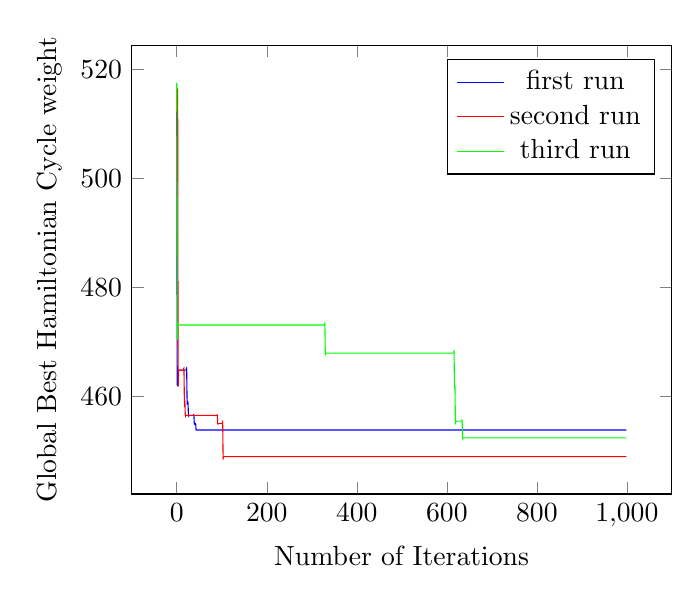
\begin{tikzpicture}
\begin{axis}[
    xlabel={Number of Iterations},
    ylabel={Global Best Hamiltonian Cycle weight},
    legend pos=north east,
    smooth
]
 
\addplot[
    color=blue,smooth
    ]
    coordinates {
  (0,513.610006884723)(1,464.82245950299443)(2,464.82245950299443)(3,464.82245950299443)(4,464.82245950299443)(5,464.82245950299443)(6,464.82245950299443)(7,464.82245950299443)(8,464.82245950299443)(9,464.82245950299443)(10,464.82245950299443)(11,464.82245950299443)(12,464.82245950299443)(13,464.82245950299443)(14,464.82245950299443)(15,464.82245950299443)(16,464.82245950299443)(17,464.82245950299443)(18,464.82245950299443)(19,464.82245950299443)(20,464.82245950299443)(21,464.82245950299443)(22,464.82245950299443)(23,459.0824085546931)(24,459.0824085546931)(25,458.7698459134533)(26,456.51526702836867)(27,456.51526702836867)(28,456.51526702836867)(29,456.51526702836867)(30,456.51526702836867)(31,456.51526702836867)(32,456.5152670283686)(33,456.5152670283686)(34,456.5152670283686)(35,456.5152670283686)(36,456.5152670283686)(37,456.5152670283686)(38,456.5152670283686)(39,454.98726096225937)(40,454.98726096225937)(41,454.98726096225937)(42,454.98726096225926)(43,453.8170850811243)(44,453.8170850811243)(45,453.8170850811243)(46,453.8170850811243)(47,453.8170850811243)(48,453.8170850811243)(49,453.8170850811243)(50,453.8170850811243)(51,453.8170850811243)(52,453.8170850811243)(53,453.8170850811242)(54,453.8170850811242)(55,453.8170850811242)(56,453.8170850811242)(57,453.8170850811242)(58,453.8170850811242)(59,453.8170850811242)(60,453.8170850811242)(61,453.8170850811242)(62,453.81708508112416)(63,453.81708508112416)(64,453.81708508112416)(65,453.81708508112416)(66,453.81708508112416)(67,453.81708508112416)(68,453.81708508112416)(69,453.81708508112416)(70,453.81708508112416)(71,453.81708508112416)(72,453.81708508112416)(73,453.81708508112416)(74,453.81708508112416)(75,453.81708508112416)(76,453.81708508112416)(77,453.81708508112416)(78,453.81708508112416)(79,453.81708508112416)(80,453.81708508112416)(81,453.81708508112416)(82,453.81708508112416)(83,453.81708508112416)(84,453.81708508112416)(85,453.81708508112416)(86,453.81708508112416)(87,453.81708508112416)(88,453.81708508112416)(89,453.81708508112416)(90,453.81708508112416)(91,453.81708508112416)(92,453.81708508112416)(93,453.81708508112416)(94,453.81708508112416)(95,453.81708508112416)(96,453.81708508112416)(97,453.81708508112416)(98,453.8170850811241)(99,453.8170850811241)(100,453.8170850811241)(101,453.8170850811241)(102,453.8170850811241)(103,453.8170850811241)(104,453.8170850811241)(105,453.8170850811241)(106,453.8170850811241)(107,453.8170850811241)(108,453.8170850811241)(109,453.8170850811241)(110,453.8170850811241)(111,453.8170850811241)(112,453.8170850811241)(113,453.8170850811241)(114,453.8170850811241)(115,453.8170850811241)(116,453.8170850811241)(117,453.8170850811241)(118,453.8170850811241)(119,453.8170850811241)(120,453.8170850811241)(121,453.8170850811241)(122,453.8170850811241)(123,453.8170850811241)(124,453.8170850811241)(125,453.8170850811241)(126,453.8170850811241)(127,453.8170850811241)(128,453.8170850811241)(129,453.8170850811241)(130,453.8170850811241)(131,453.8170850811241)(132,453.8170850811241)(133,453.8170850811241)(134,453.8170850811241)(135,453.8170850811241)(136,453.8170850811241)(137,453.8170850811241)(138,453.8170850811241)(139,453.8170850811241)(140,453.8170850811241)(141,453.8170850811241)(142,453.8170850811241)(143,453.8170850811241)(144,453.8170850811241)(145,453.8170850811241)(146,453.8170850811241)(147,453.8170850811241)(148,453.8170850811241)(149,453.8170850811241)(150,453.8170850811241)(151,453.8170850811241)(152,453.8170850811241)(153,453.8170850811241)(154,453.8170850811241)(155,453.8170850811241)(156,453.8170850811241)(157,453.8170850811241)(158,453.8170850811241)(159,453.8170850811241)(160,453.8170850811241)(161,453.8170850811241)(162,453.8170850811241)(163,453.8170850811241)(164,453.8170850811241)(165,453.8170850811241)(166,453.8170850811241)(167,453.8170850811241)(168,453.8170850811241)(169,453.8170850811241)(170,453.8170850811241)(171,453.8170850811241)(172,453.8170850811241)(173,453.8170850811241)(174,453.8170850811241)(175,453.8170850811241)(176,453.8170850811241)(177,453.8170850811241)(178,453.8170850811241)(179,453.8170850811241)(180,453.8170850811241)(181,453.8170850811241)(182,453.8170850811241)(183,453.8170850811241)(184,453.8170850811241)(185,453.8170850811241)(186,453.8170850811241)(187,453.8170850811241)(188,453.8170850811241)(189,453.8170850811241)(190,453.8170850811241)(191,453.8170850811241)(192,453.8170850811241)(193,453.8170850811241)(194,453.8170850811241)(195,453.8170850811241)(196,453.8170850811241)(197,453.8170850811241)(198,453.8170850811241)(199,453.8170850811241)(200,453.8170850811241)(201,453.8170850811241)(202,453.8170850811241)(203,453.8170850811241)(204,453.8170850811241)(205,453.8170850811241)(206,453.8170850811241)(207,453.8170850811241)(208,453.8170850811241)(209,453.8170850811241)(210,453.8170850811241)(211,453.8170850811241)(212,453.8170850811241)(213,453.8170850811241)(214,453.8170850811241)(215,453.8170850811241)(216,453.8170850811241)(217,453.8170850811241)(218,453.8170850811241)(219,453.8170850811241)(220,453.8170850811241)(221,453.8170850811241)(222,453.8170850811241)(223,453.8170850811241)(224,453.8170850811241)(225,453.8170850811241)(226,453.8170850811241)(227,453.8170850811241)(228,453.8170850811241)(229,453.8170850811241)(230,453.8170850811241)(231,453.8170850811241)(232,453.8170850811241)(233,453.8170850811241)(234,453.8170850811241)(235,453.8170850811241)(236,453.8170850811241)(237,453.8170850811241)(238,453.8170850811241)(239,453.8170850811241)(240,453.8170850811241)(241,453.8170850811241)(242,453.8170850811241)(243,453.8170850811241)(244,453.8170850811241)(245,453.8170850811241)(246,453.8170850811241)(247,453.8170850811241)(248,453.8170850811241)(249,453.8170850811241)(250,453.8170850811241)(251,453.8170850811241)(252,453.8170850811241)(253,453.8170850811241)(254,453.8170850811241)(255,453.8170850811241)(256,453.8170850811241)(257,453.8170850811241)(258,453.8170850811241)(259,453.8170850811241)(260,453.8170850811241)(261,453.8170850811241)(262,453.8170850811241)(263,453.8170850811241)(264,453.8170850811241)(265,453.8170850811241)(266,453.8170850811241)(267,453.8170850811241)(268,453.8170850811241)(269,453.8170850811241)(270,453.8170850811241)(271,453.8170850811241)(272,453.8170850811241)(273,453.8170850811241)(274,453.8170850811241)(275,453.8170850811241)(276,453.8170850811241)(277,453.8170850811241)(278,453.8170850811241)(279,453.8170850811241)(280,453.8170850811241)(281,453.8170850811241)(282,453.8170850811241)(283,453.8170850811241)(284,453.8170850811241)(285,453.8170850811241)(286,453.8170850811241)(287,453.8170850811241)(288,453.8170850811241)(289,453.8170850811241)(290,453.8170850811241)(291,453.8170850811241)(292,453.8170850811241)(293,453.8170850811241)(294,453.8170850811241)(295,453.8170850811241)(296,453.8170850811241)(297,453.8170850811241)(298,453.8170850811241)(299,453.8170850811241)(300,453.8170850811241)(301,453.8170850811241)(302,453.8170850811241)(303,453.8170850811241)(304,453.8170850811241)(305,453.8170850811241)(306,453.8170850811241)(307,453.8170850811241)(308,453.8170850811241)(309,453.8170850811241)(310,453.8170850811241)(311,453.8170850811241)(312,453.8170850811241)(313,453.8170850811241)(314,453.8170850811241)(315,453.8170850811241)(316,453.8170850811241)(317,453.8170850811241)(318,453.8170850811241)(319,453.8170850811241)(320,453.8170850811241)(321,453.8170850811241)(322,453.8170850811241)(323,453.8170850811241)(324,453.8170850811241)(325,453.8170850811241)(326,453.8170850811241)(327,453.8170850811241)(328,453.8170850811241)(329,453.8170850811241)(330,453.8170850811241)(331,453.8170850811241)(332,453.8170850811241)(333,453.8170850811241)(334,453.8170850811241)(335,453.8170850811241)(336,453.8170850811241)(337,453.8170850811241)(338,453.8170850811241)(339,453.8170850811241)(340,453.8170850811241)(341,453.8170850811241)(342,453.8170850811241)(343,453.8170850811241)(344,453.8170850811241)(345,453.8170850811241)(346,453.8170850811241)(347,453.8170850811241)(348,453.8170850811241)(349,453.8170850811241)(350,453.8170850811241)(351,453.8170850811241)(352,453.8170850811241)(353,453.8170850811241)(354,453.8170850811241)(355,453.8170850811241)(356,453.8170850811241)(357,453.8170850811241)(358,453.8170850811241)(359,453.8170850811241)(360,453.8170850811241)(361,453.8170850811241)(362,453.8170850811241)(363,453.8170850811241)(364,453.8170850811241)(365,453.8170850811241)(366,453.8170850811241)(367,453.8170850811241)(368,453.8170850811241)(369,453.8170850811241)(370,453.8170850811241)(371,453.8170850811241)(372,453.8170850811241)(373,453.8170850811241)(374,453.8170850811241)(375,453.8170850811241)(376,453.8170850811241)(377,453.8170850811241)(378,453.8170850811241)(379,453.8170850811241)(380,453.8170850811241)(381,453.8170850811241)(382,453.8170850811241)(383,453.8170850811241)(384,453.8170850811241)(385,453.8170850811241)(386,453.8170850811241)(387,453.8170850811241)(388,453.8170850811241)(389,453.8170850811241)(390,453.8170850811241)(391,453.8170850811241)(392,453.8170850811241)(393,453.8170850811241)(394,453.8170850811241)(395,453.8170850811241)(396,453.8170850811241)(397,453.8170850811241)(398,453.8170850811241)(399,453.8170850811241)(400,453.8170850811241)(401,453.8170850811241)(402,453.8170850811241)(403,453.8170850811241)(404,453.8170850811241)(405,453.8170850811241)(406,453.8170850811241)(407,453.8170850811241)(408,453.8170850811241)(409,453.8170850811241)(410,453.8170850811241)(411,453.8170850811241)(412,453.8170850811241)(413,453.8170850811241)(414,453.8170850811241)(415,453.8170850811241)(416,453.8170850811241)(417,453.8170850811241)(418,453.8170850811241)(419,453.8170850811241)(420,453.8170850811241)(421,453.8170850811241)(422,453.8170850811241)(423,453.8170850811241)(424,453.8170850811241)(425,453.8170850811241)(426,453.8170850811241)(427,453.8170850811241)(428,453.8170850811241)(429,453.8170850811241)(430,453.8170850811241)(431,453.8170850811241)(432,453.8170850811241)(433,453.8170850811241)(434,453.8170850811241)(435,453.8170850811241)(436,453.8170850811241)(437,453.8170850811241)(438,453.8170850811241)(439,453.8170850811241)(440,453.8170850811241)(441,453.8170850811241)(442,453.8170850811241)(443,453.8170850811241)(444,453.8170850811241)(445,453.8170850811241)(446,453.8170850811241)(447,453.8170850811241)(448,453.8170850811241)(449,453.8170850811241)(450,453.8170850811241)(451,453.8170850811241)(452,453.8170850811241)(453,453.8170850811241)(454,453.8170850811241)(455,453.8170850811241)(456,453.8170850811241)(457,453.8170850811241)(458,453.8170850811241)(459,453.8170850811241)(460,453.8170850811241)(461,453.8170850811241)(462,453.8170850811241)(463,453.8170850811241)(464,453.8170850811241)(465,453.8170850811241)(466,453.8170850811241)(467,453.8170850811241)(468,453.8170850811241)(469,453.8170850811241)(470,453.8170850811241)(471,453.8170850811241)(472,453.8170850811241)(473,453.8170850811241)(474,453.8170850811241)(475,453.8170850811241)(476,453.8170850811241)(477,453.8170850811241)(478,453.8170850811241)(479,453.8170850811241)(480,453.8170850811241)(481,453.8170850811241)(482,453.8170850811241)(483,453.8170850811241)(484,453.8170850811241)(485,453.8170850811241)(486,453.8170850811241)(487,453.8170850811241)(488,453.8170850811241)(489,453.8170850811241)(490,453.8170850811241)(491,453.8170850811241)(492,453.8170850811241)(493,453.8170850811241)(494,453.8170850811241)(495,453.8170850811241)(496,453.8170850811241)(497,453.8170850811241)(498,453.8170850811241)(499,453.8170850811241)(500,453.8170850811241)(501,453.8170850811241)(502,453.8170850811241)(503,453.8170850811241)(504,453.8170850811241)(505,453.8170850811241)(506,453.8170850811241)(507,453.8170850811241)(508,453.8170850811241)(509,453.8170850811241)(510,453.8170850811241)(511,453.8170850811241)(512,453.8170850811241)(513,453.8170850811241)(514,453.8170850811241)(515,453.8170850811241)(516,453.8170850811241)(517,453.8170850811241)(518,453.8170850811241)(519,453.8170850811241)(520,453.8170850811241)(521,453.8170850811241)(522,453.8170850811241)(523,453.8170850811241)(524,453.8170850811241)(525,453.8170850811241)(526,453.8170850811241)(527,453.8170850811241)(528,453.8170850811241)(529,453.8170850811241)(530,453.8170850811241)(531,453.8170850811241)(532,453.8170850811241)(533,453.8170850811241)(534,453.8170850811241)(535,453.8170850811241)(536,453.8170850811241)(537,453.8170850811241)(538,453.8170850811241)(539,453.8170850811241)(540,453.8170850811241)(541,453.8170850811241)(542,453.8170850811241)(543,453.8170850811241)(544,453.8170850811241)(545,453.8170850811241)(546,453.8170850811241)(547,453.8170850811241)(548,453.8170850811241)(549,453.8170850811241)(550,453.8170850811241)(551,453.8170850811241)(552,453.8170850811241)(553,453.8170850811241)(554,453.8170850811241)(555,453.8170850811241)(556,453.8170850811241)(557,453.8170850811241)(558,453.8170850811241)(559,453.8170850811241)(560,453.8170850811241)(561,453.8170850811241)(562,453.8170850811241)(563,453.8170850811241)(564,453.8170850811241)(565,453.8170850811241)(566,453.8170850811241)(567,453.8170850811241)(568,453.8170850811241)(569,453.8170850811241)(570,453.8170850811241)(571,453.8170850811241)(572,453.8170850811241)(573,453.8170850811241)(574,453.8170850811241)(575,453.8170850811241)(576,453.8170850811241)(577,453.8170850811241)(578,453.8170850811241)(579,453.8170850811241)(580,453.8170850811241)(581,453.8170850811241)(582,453.8170850811241)(583,453.8170850811241)(584,453.8170850811241)(585,453.8170850811241)(586,453.8170850811241)(587,453.8170850811241)(588,453.8170850811241)(589,453.8170850811241)(590,453.8170850811241)(591,453.8170850811241)(592,453.8170850811241)(593,453.8170850811241)(594,453.8170850811241)(595,453.8170850811241)(596,453.8170850811241)(597,453.8170850811241)(598,453.8170850811241)(599,453.8170850811241)(600,453.8170850811241)(601,453.8170850811241)(602,453.8170850811241)(603,453.8170850811241)(604,453.8170850811241)(605,453.8170850811241)(606,453.8170850811241)(607,453.8170850811241)(608,453.8170850811241)(609,453.8170850811241)(610,453.8170850811241)(611,453.8170850811241)(612,453.8170850811241)(613,453.8170850811241)(614,453.8170850811241)(615,453.8170850811241)(616,453.8170850811241)(617,453.8170850811241)(618,453.8170850811241)(619,453.8170850811241)(620,453.8170850811241)(621,453.8170850811241)(622,453.8170850811241)(623,453.8170850811241)(624,453.8170850811241)(625,453.8170850811241)(626,453.8170850811241)(627,453.8170850811241)(628,453.8170850811241)(629,453.8170850811241)(630,453.8170850811241)(631,453.8170850811241)(632,453.8170850811241)(633,453.8170850811241)(634,453.8170850811241)(635,453.8170850811241)(636,453.8170850811241)(637,453.8170850811241)(638,453.8170850811241)(639,453.8170850811241)(640,453.8170850811241)(641,453.8170850811241)(642,453.8170850811241)(643,453.8170850811241)(644,453.8170850811241)(645,453.8170850811241)(646,453.8170850811241)(647,453.8170850811241)(648,453.8170850811241)(649,453.8170850811241)(650,453.8170850811241)(651,453.8170850811241)(652,453.8170850811241)(653,453.8170850811241)(654,453.8170850811241)(655,453.8170850811241)(656,453.8170850811241)(657,453.8170850811241)(658,453.8170850811241)(659,453.8170850811241)(660,453.8170850811241)(661,453.8170850811241)(662,453.8170850811241)(663,453.8170850811241)(664,453.8170850811241)(665,453.8170850811241)(666,453.8170850811241)(667,453.8170850811241)(668,453.8170850811241)(669,453.8170850811241)(670,453.8170850811241)(671,453.8170850811241)(672,453.8170850811241)(673,453.8170850811241)(674,453.8170850811241)(675,453.8170850811241)(676,453.8170850811241)(677,453.8170850811241)(678,453.8170850811241)(679,453.8170850811241)(680,453.8170850811241)(681,453.8170850811241)(682,453.8170850811241)(683,453.8170850811241)(684,453.8170850811241)(685,453.8170850811241)(686,453.8170850811241)(687,453.8170850811241)(688,453.8170850811241)(689,453.8170850811241)(690,453.8170850811241)(691,453.8170850811241)(692,453.8170850811241)(693,453.8170850811241)(694,453.8170850811241)(695,453.8170850811241)(696,453.8170850811241)(697,453.8170850811241)(698,453.8170850811241)(699,453.8170850811241)(700,453.8170850811241)(701,453.8170850811241)(702,453.8170850811241)(703,453.8170850811241)(704,453.8170850811241)(705,453.8170850811241)(706,453.8170850811241)(707,453.8170850811241)(708,453.8170850811241)(709,453.8170850811241)(710,453.8170850811241)(711,453.8170850811241)(712,453.8170850811241)(713,453.8170850811241)(714,453.8170850811241)(715,453.8170850811241)(716,453.8170850811241)(717,453.8170850811241)(718,453.8170850811241)(719,453.8170850811241)(720,453.8170850811241)(721,453.8170850811241)(722,453.8170850811241)(723,453.8170850811241)(724,453.8170850811241)(725,453.8170850811241)(726,453.8170850811241)(727,453.8170850811241)(728,453.8170850811241)(729,453.8170850811241)(730,453.8170850811241)(731,453.8170850811241)(732,453.8170850811241)(733,453.8170850811241)(734,453.8170850811241)(735,453.8170850811241)(736,453.8170850811241)(737,453.8170850811241)(738,453.8170850811241)(739,453.8170850811241)(740,453.8170850811241)(741,453.8170850811241)(742,453.8170850811241)(743,453.8170850811241)(744,453.8170850811241)(745,453.8170850811241)(746,453.8170850811241)(747,453.8170850811241)(748,453.8170850811241)(749,453.8170850811241)(750,453.8170850811241)(751,453.8170850811241)(752,453.8170850811241)(753,453.8170850811241)(754,453.8170850811241)(755,453.8170850811241)(756,453.8170850811241)(757,453.8170850811241)(758,453.8170850811241)(759,453.8170850811241)(760,453.8170850811241)(761,453.8170850811241)(762,453.8170850811241)(763,453.8170850811241)(764,453.8170850811241)(765,453.8170850811241)(766,453.8170850811241)(767,453.8170850811241)(768,453.8170850811241)(769,453.8170850811241)(770,453.8170850811241)(771,453.8170850811241)(772,453.8170850811241)(773,453.8170850811241)(774,453.8170850811241)(775,453.8170850811241)(776,453.8170850811241)(777,453.8170850811241)(778,453.8170850811241)(779,453.8170850811241)(780,453.8170850811241)(781,453.8170850811241)(782,453.8170850811241)(783,453.8170850811241)(784,453.8170850811241)(785,453.8170850811241)(786,453.8170850811241)(787,453.8170850811241)(788,453.8170850811241)(789,453.8170850811241)(790,453.8170850811241)(791,453.8170850811241)(792,453.8170850811241)(793,453.8170850811241)(794,453.8170850811241)(795,453.8170850811241)(796,453.8170850811241)(797,453.8170850811241)(798,453.8170850811241)(799,453.8170850811241)(800,453.8170850811241)(801,453.8170850811241)(802,453.8170850811241)(803,453.8170850811241)(804,453.8170850811241)(805,453.8170850811241)(806,453.8170850811241)(807,453.8170850811241)(808,453.8170850811241)(809,453.8170850811241)(810,453.8170850811241)(811,453.8170850811241)(812,453.8170850811241)(813,453.8170850811241)(814,453.8170850811241)(815,453.8170850811241)(816,453.8170850811241)(817,453.8170850811241)(818,453.8170850811241)(819,453.8170850811241)(820,453.8170850811241)(821,453.8170850811241)(822,453.8170850811241)(823,453.8170850811241)(824,453.8170850811241)(825,453.8170850811241)(826,453.8170850811241)(827,453.8170850811241)(828,453.8170850811241)(829,453.8170850811241)(830,453.8170850811241)(831,453.8170850811241)(832,453.8170850811241)(833,453.8170850811241)(834,453.8170850811241)(835,453.8170850811241)(836,453.8170850811241)(837,453.8170850811241)(838,453.8170850811241)(839,453.8170850811241)(840,453.8170850811241)(841,453.8170850811241)(842,453.8170850811241)(843,453.8170850811241)(844,453.8170850811241)(845,453.8170850811241)(846,453.8170850811241)(847,453.8170850811241)(848,453.8170850811241)(849,453.8170850811241)(850,453.8170850811241)(851,453.8170850811241)(852,453.8170850811241)(853,453.8170850811241)(854,453.8170850811241)(855,453.8170850811241)(856,453.8170850811241)(857,453.8170850811241)(858,453.8170850811241)(859,453.8170850811241)(860,453.8170850811241)(861,453.8170850811241)(862,453.8170850811241)(863,453.8170850811241)(864,453.8170850811241)(865,453.8170850811241)(866,453.8170850811241)(867,453.8170850811241)(868,453.8170850811241)(869,453.8170850811241)(870,453.8170850811241)(871,453.8170850811241)(872,453.8170850811241)(873,453.8170850811241)(874,453.8170850811241)(875,453.8170850811241)(876,453.8170850811241)(877,453.8170850811241)(878,453.8170850811241)(879,453.8170850811241)(880,453.8170850811241)(881,453.8170850811241)(882,453.8170850811241)(883,453.8170850811241)(884,453.8170850811241)(885,453.8170850811241)(886,453.8170850811241)(887,453.8170850811241)(888,453.8170850811241)(889,453.8170850811241)(890,453.8170850811241)(891,453.8170850811241)(892,453.8170850811241)(893,453.8170850811241)(894,453.8170850811241)(895,453.8170850811241)(896,453.8170850811241)(897,453.8170850811241)(898,453.8170850811241)(899,453.8170850811241)(900,453.8170850811241)(901,453.8170850811241)(902,453.8170850811241)(903,453.8170850811241)(904,453.8170850811241)(905,453.8170850811241)(906,453.8170850811241)(907,453.8170850811241)(908,453.8170850811241)(909,453.8170850811241)(910,453.8170850811241)(911,453.8170850811241)(912,453.8170850811241)(913,453.8170850811241)(914,453.8170850811241)(915,453.8170850811241)(916,453.8170850811241)(917,453.8170850811241)(918,453.8170850811241)(919,453.8170850811241)(920,453.8170850811241)(921,453.8170850811241)(922,453.8170850811241)(923,453.8170850811241)(924,453.8170850811241)(925,453.8170850811241)(926,453.8170850811241)(927,453.8170850811241)(928,453.8170850811241)(929,453.8170850811241)(930,453.8170850811241)(931,453.8170850811241)(932,453.8170850811241)(933,453.8170850811241)(934,453.8170850811241)(935,453.8170850811241)(936,453.8170850811241)(937,453.8170850811241)(938,453.8170850811241)(939,453.8170850811241)(940,453.8170850811241)(941,453.8170850811241)(942,453.8170850811241)(943,453.8170850811241)(944,453.8170850811241)(945,453.8170850811241)(946,453.8170850811241)(947,453.8170850811241)(948,453.8170850811241)(949,453.8170850811241)(950,453.8170850811241)(951,453.8170850811241)(952,453.8170850811241)(953,453.8170850811241)(954,453.8170850811241)(955,453.8170850811241)(956,453.8170850811241)(957,453.8170850811241)(958,453.8170850811241)(959,453.8170850811241)(960,453.8170850811241)(961,453.8170850811241)(962,453.8170850811241)(963,453.8170850811241)(964,453.8170850811241)(965,453.8170850811241)(966,453.8170850811241)(967,453.8170850811241)(968,453.8170850811241)(969,453.8170850811241)(970,453.8170850811241)(971,453.8170850811241)(972,453.8170850811241)(973,453.8170850811241)(974,453.8170850811241)(975,453.8170850811241)(976,453.8170850811241)(977,453.8170850811241)(978,453.8170850811241)(979,453.8170850811241)(980,453.8170850811241)(981,453.8170850811241)(982,453.8170850811241)(983,453.8170850811241)(984,453.8170850811241)(985,453.8170850811241)(986,453.8170850811241)(987,453.8170850811241)(988,453.8170850811241)(989,453.8170850811241)(990,453.8170850811241)(991,453.8170850811241)(992,453.8170850811241)(993,453.8170850811241)(994,453.8170850811241)(995,453.8170850811241)(996,453.8170850811241)(997,453.8170850811241)(998,453.8170850811241)(999,453.8170850811241)
    };
   \addlegendentry{first run}
\addplot[
    color=red,smooth
    ]
    coordinates {(0,513.610006884723)(1,513.610006884723)(2,513.610006884723)(3,464.82245950299443)(4,464.82245950299443)(5,464.82245950299443)(6,464.82245950299443)(7,464.82245950299443)(8,464.82245950299443)(9,464.82245950299443)(10,464.82245950299443)(11,464.82245950299443)(12,464.82245950299443)(13,464.82245950299443)(14,464.82245950299443)(15,464.82245950299443)(16,464.82245950299443)(17,459.0824085546931)(18,459.0824085546931)(19,456.51526702836867)(20,456.51526702836867)(21,456.51526702836867)(22,456.51526702836867)(23,456.51526702836867)(24,456.51526702836867)(25,456.51526702836867)(26,456.51526702836867)(27,456.51526702836867)(28,456.51526702836867)(29,456.51526702836867)(30,456.51526702836867)(31,456.51526702836867)(32,456.51526702836867)(33,456.51526702836867)(34,456.51526702836867)(35,456.5152670283686)(36,456.5152670283686)(37,456.5152670283686)(38,456.5152670283686)(39,456.5152670283686)(40,456.5152670283686)(41,456.51526702836856)(42,456.51526702836856)(43,456.51526702836856)(44,456.51526702836856)(45,456.51526702836856)(46,456.51526702836856)(47,456.51526702836856)(48,456.51526702836856)(49,456.51526702836856)(50,456.51526702836856)(51,456.51526702836856)(52,456.51526702836856)(53,456.51526702836856)(54,456.51526702836856)(55,456.51526702836856)(56,456.51526702836856)(57,456.51526702836856)(58,456.51526702836856)(59,456.51526702836856)(60,456.51526702836856)(61,456.51526702836856)(62,456.51526702836856)(63,456.51526702836856)(64,456.51526702836856)(65,456.51526702836856)(66,456.51526702836856)(67,456.51526702836856)(68,456.51526702836856)(69,456.51526702836856)(70,456.51526702836856)(71,456.51526702836856)(72,456.51526702836856)(73,456.51526702836856)(74,456.51526702836856)(75,456.51526702836856)(76,456.51526702836856)(77,456.51526702836856)(78,456.51526702836856)(79,456.51526702836856)(80,456.51526702836856)(81,456.51526702836856)(82,456.51526702836856)(83,456.51526702836856)(84,456.51526702836856)(85,456.51526702836856)(86,456.51526702836856)(87,456.51526702836856)(88,456.51526702836856)(89,456.51526702836856)(90,456.51526702836856)(91,454.98726096225937)(92,454.98726096225937)(93,454.98726096225926)(94,454.98726096225926)(95,454.98726096225926)(96,454.98726096225926)(97,454.98726096225926)(98,454.98726096225926)(99,454.98726096225926)(100,454.98726096225926)(101,454.98726096225926)(102,454.98726096225926)(103,448.93640451228947)(104,448.93640451228947)(105,448.93640451228947)(106,448.93640451228947)(107,448.93640451228947)(108,448.93640451228947)(109,448.93640451228947)(110,448.93640451228947)(111,448.93640451228947)(112,448.9364045122893)(113,448.9364045122893)(114,448.9364045122893)(115,448.9364045122893)(116,448.9364045122893)(117,448.9364045122893)(118,448.9364045122893)(119,448.9364045122893)(120,448.9364045122893)(121,448.9364045122893)(122,448.9364045122893)(123,448.9364045122893)(124,448.9364045122893)(125,448.9364045122893)(126,448.9364045122893)(127,448.9364045122893)(128,448.9364045122893)(129,448.9364045122893)(130,448.9364045122893)(131,448.9364045122893)(132,448.9364045122893)(133,448.9364045122893)(134,448.9364045122893)(135,448.9364045122893)(136,448.9364045122893)(137,448.9364045122893)(138,448.9364045122893)(139,448.9364045122893)(140,448.9364045122893)(141,448.9364045122893)(142,448.9364045122893)(143,448.9364045122893)(144,448.9364045122893)(145,448.9364045122893)(146,448.9364045122893)(147,448.9364045122893)(148,448.9364045122893)(149,448.9364045122893)(150,448.9364045122893)(151,448.9364045122893)(152,448.9364045122893)(153,448.9364045122893)(154,448.9364045122893)(155,448.9364045122893)(156,448.9364045122893)(157,448.9364045122893)(158,448.9364045122893)(159,448.9364045122893)(160,448.9364045122893)(161,448.9364045122893)(162,448.9364045122893)(163,448.9364045122893)(164,448.9364045122893)(165,448.9364045122893)(166,448.9364045122893)(167,448.9364045122893)(168,448.9364045122893)(169,448.9364045122893)(170,448.9364045122893)(171,448.9364045122893)(172,448.9364045122893)(173,448.9364045122893)(174,448.9364045122893)(175,448.9364045122893)(176,448.9364045122893)(177,448.9364045122893)(178,448.9364045122893)(179,448.9364045122893)(180,448.93640451228924)(181,448.93640451228924)(182,448.93640451228924)(183,448.93640451228924)(184,448.93640451228924)(185,448.93640451228924)(186,448.93640451228924)(187,448.93640451228924)(188,448.93640451228924)(189,448.93640451228924)(190,448.93640451228924)(191,448.93640451228924)(192,448.93640451228924)(193,448.93640451228924)(194,448.93640451228924)(195,448.93640451228924)(196,448.93640451228924)(197,448.93640451228924)(198,448.93640451228924)(199,448.93640451228924)(200,448.93640451228924)(201,448.93640451228924)(202,448.93640451228924)(203,448.93640451228924)(204,448.93640451228924)(205,448.93640451228924)(206,448.93640451228924)(207,448.93640451228924)(208,448.93640451228924)(209,448.93640451228924)(210,448.93640451228924)(211,448.93640451228924)(212,448.93640451228924)(213,448.93640451228924)(214,448.93640451228924)(215,448.93640451228924)(216,448.93640451228924)(217,448.93640451228924)(218,448.93640451228924)(219,448.93640451228924)(220,448.93640451228924)(221,448.93640451228924)(222,448.93640451228924)(223,448.93640451228924)(224,448.93640451228924)(225,448.93640451228924)(226,448.93640451228924)(227,448.93640451228924)(228,448.93640451228924)(229,448.93640451228924)(230,448.93640451228924)(231,448.93640451228924)(232,448.93640451228924)(233,448.93640451228924)(234,448.93640451228924)(235,448.93640451228924)(236,448.93640451228924)(237,448.93640451228924)(238,448.93640451228924)(239,448.93640451228924)(240,448.93640451228924)(241,448.93640451228924)(242,448.93640451228924)(243,448.93640451228924)(244,448.93640451228924)(245,448.93640451228924)(246,448.93640451228924)(247,448.93640451228924)(248,448.93640451228924)(249,448.93640451228924)(250,448.93640451228924)(251,448.93640451228924)(252,448.93640451228924)(253,448.93640451228924)(254,448.93640451228924)(255,448.93640451228924)(256,448.93640451228924)(257,448.93640451228924)(258,448.93640451228924)(259,448.93640451228924)(260,448.93640451228924)(261,448.93640451228924)(262,448.93640451228924)(263,448.93640451228924)(264,448.93640451228924)(265,448.93640451228924)(266,448.93640451228924)(267,448.93640451228924)(268,448.93640451228924)(269,448.93640451228924)(270,448.93640451228924)(271,448.93640451228924)(272,448.93640451228924)(273,448.93640451228924)(274,448.93640451228924)(275,448.93640451228924)(276,448.93640451228924)(277,448.93640451228924)(278,448.93640451228924)(279,448.93640451228924)(280,448.93640451228924)(281,448.93640451228924)(282,448.93640451228924)(283,448.93640451228924)(284,448.93640451228924)(285,448.93640451228924)(286,448.93640451228924)(287,448.93640451228924)(288,448.93640451228924)(289,448.93640451228924)(290,448.93640451228924)(291,448.93640451228924)(292,448.93640451228924)(293,448.93640451228924)(294,448.93640451228924)(295,448.93640451228924)(296,448.93640451228924)(297,448.93640451228924)(298,448.93640451228924)(299,448.93640451228924)(300,448.93640451228924)(301,448.93640451228924)(302,448.93640451228924)(303,448.93640451228924)(304,448.93640451228924)(305,448.93640451228924)(306,448.93640451228924)(307,448.93640451228924)(308,448.93640451228924)(309,448.93640451228924)(310,448.93640451228924)(311,448.93640451228924)(312,448.93640451228924)(313,448.93640451228924)(314,448.93640451228924)(315,448.93640451228924)(316,448.93640451228924)(317,448.93640451228924)(318,448.93640451228924)(319,448.93640451228924)(320,448.93640451228924)(321,448.93640451228924)(322,448.93640451228924)(323,448.93640451228924)(324,448.93640451228924)(325,448.93640451228924)(326,448.93640451228924)(327,448.93640451228924)(328,448.93640451228924)(329,448.93640451228924)(330,448.93640451228924)(331,448.93640451228924)(332,448.93640451228924)(333,448.93640451228924)(334,448.93640451228924)(335,448.93640451228924)(336,448.93640451228924)(337,448.93640451228924)(338,448.93640451228924)(339,448.93640451228924)(340,448.93640451228924)(341,448.93640451228924)(342,448.93640451228924)(343,448.93640451228924)(344,448.93640451228924)(345,448.93640451228924)(346,448.93640451228924)(347,448.93640451228924)(348,448.93640451228924)(349,448.93640451228924)(350,448.93640451228924)(351,448.93640451228924)(352,448.93640451228924)(353,448.93640451228924)(354,448.93640451228924)(355,448.93640451228924)(356,448.93640451228924)(357,448.93640451228924)(358,448.93640451228924)(359,448.93640451228924)(360,448.93640451228924)(361,448.93640451228924)(362,448.93640451228924)(363,448.93640451228924)(364,448.93640451228924)(365,448.93640451228924)(366,448.93640451228924)(367,448.93640451228924)(368,448.93640451228924)(369,448.93640451228924)(370,448.93640451228924)(371,448.93640451228924)(372,448.93640451228924)(373,448.93640451228924)(374,448.93640451228924)(375,448.93640451228924)(376,448.93640451228924)(377,448.93640451228924)(378,448.93640451228924)(379,448.93640451228924)(380,448.93640451228924)(381,448.93640451228924)(382,448.93640451228924)(383,448.93640451228924)(384,448.93640451228924)(385,448.93640451228924)(386,448.93640451228924)(387,448.93640451228924)(388,448.93640451228924)(389,448.93640451228924)(390,448.93640451228924)(391,448.93640451228924)(392,448.93640451228924)(393,448.93640451228924)(394,448.93640451228924)(395,448.93640451228924)(396,448.93640451228924)(397,448.93640451228924)(398,448.93640451228924)(399,448.93640451228924)(400,448.93640451228924)(401,448.93640451228924)(402,448.93640451228924)(403,448.93640451228924)(404,448.93640451228924)(405,448.93640451228924)(406,448.93640451228924)(407,448.93640451228924)(408,448.93640451228924)(409,448.93640451228924)(410,448.93640451228924)(411,448.93640451228924)(412,448.93640451228924)(413,448.93640451228924)(414,448.93640451228924)(415,448.93640451228924)(416,448.93640451228924)(417,448.93640451228924)(418,448.93640451228924)(419,448.93640451228924)(420,448.93640451228924)(421,448.93640451228924)(422,448.93640451228924)(423,448.93640451228924)(424,448.93640451228924)(425,448.93640451228924)(426,448.93640451228924)(427,448.93640451228924)(428,448.93640451228924)(429,448.93640451228924)(430,448.93640451228924)(431,448.93640451228924)(432,448.93640451228924)(433,448.93640451228924)(434,448.93640451228924)(435,448.93640451228924)(436,448.93640451228924)(437,448.93640451228924)(438,448.93640451228924)(439,448.93640451228924)(440,448.93640451228924)(441,448.93640451228924)(442,448.93640451228924)(443,448.93640451228924)(444,448.93640451228924)(445,448.93640451228924)(446,448.93640451228924)(447,448.93640451228924)(448,448.93640451228924)(449,448.93640451228924)(450,448.93640451228924)(451,448.93640451228924)(452,448.93640451228924)(453,448.93640451228924)(454,448.93640451228924)(455,448.93640451228924)(456,448.93640451228924)(457,448.93640451228924)(458,448.93640451228924)(459,448.93640451228924)(460,448.93640451228924)(461,448.93640451228924)(462,448.93640451228924)(463,448.93640451228924)(464,448.93640451228924)(465,448.93640451228924)(466,448.93640451228924)(467,448.93640451228924)(468,448.93640451228924)(469,448.93640451228924)(470,448.93640451228924)(471,448.93640451228924)(472,448.93640451228924)(473,448.93640451228924)(474,448.93640451228924)(475,448.93640451228924)(476,448.93640451228924)(477,448.93640451228924)(478,448.93640451228924)(479,448.93640451228924)(480,448.93640451228924)(481,448.93640451228924)(482,448.93640451228924)(483,448.93640451228924)(484,448.93640451228924)(485,448.93640451228924)(486,448.93640451228924)(487,448.93640451228924)(488,448.93640451228924)(489,448.93640451228924)(490,448.93640451228924)(491,448.93640451228924)(492,448.93640451228924)(493,448.93640451228924)(494,448.93640451228924)(495,448.93640451228924)(496,448.93640451228924)(497,448.93640451228924)(498,448.93640451228924)(499,448.93640451228924)(500,448.93640451228924)(501,448.93640451228924)(502,448.93640451228924)(503,448.93640451228924)(504,448.93640451228924)(505,448.93640451228924)(506,448.93640451228924)(507,448.93640451228924)(508,448.93640451228924)(509,448.93640451228924)(510,448.93640451228924)(511,448.93640451228924)(512,448.93640451228924)(513,448.93640451228924)(514,448.93640451228924)(515,448.93640451228924)(516,448.93640451228924)(517,448.93640451228924)(518,448.93640451228924)(519,448.93640451228924)(520,448.93640451228924)(521,448.93640451228924)(522,448.93640451228924)(523,448.93640451228924)(524,448.93640451228924)(525,448.93640451228924)(526,448.93640451228924)(527,448.93640451228924)(528,448.93640451228924)(529,448.93640451228924)(530,448.93640451228924)(531,448.93640451228924)(532,448.93640451228924)(533,448.93640451228924)(534,448.93640451228924)(535,448.93640451228924)(536,448.93640451228924)(537,448.93640451228924)(538,448.93640451228924)(539,448.93640451228924)(540,448.93640451228924)(541,448.93640451228924)(542,448.93640451228924)(543,448.93640451228924)(544,448.93640451228924)(545,448.93640451228924)(546,448.93640451228924)(547,448.93640451228924)(548,448.93640451228924)(549,448.93640451228924)(550,448.93640451228924)(551,448.93640451228924)(552,448.93640451228924)(553,448.93640451228924)(554,448.93640451228924)(555,448.93640451228924)(556,448.93640451228924)(557,448.93640451228924)(558,448.93640451228924)(559,448.93640451228924)(560,448.93640451228924)(561,448.93640451228924)(562,448.93640451228924)(563,448.93640451228924)(564,448.93640451228924)(565,448.93640451228924)(566,448.93640451228924)(567,448.93640451228924)(568,448.93640451228924)(569,448.93640451228924)(570,448.93640451228924)(571,448.93640451228924)(572,448.93640451228924)(573,448.93640451228924)(574,448.93640451228924)(575,448.93640451228924)(576,448.93640451228924)(577,448.93640451228924)(578,448.93640451228924)(579,448.93640451228924)(580,448.93640451228924)(581,448.93640451228924)(582,448.93640451228924)(583,448.93640451228924)(584,448.93640451228924)(585,448.93640451228924)(586,448.93640451228924)(587,448.93640451228924)(588,448.93640451228924)(589,448.93640451228924)(590,448.93640451228924)(591,448.93640451228924)(592,448.93640451228924)(593,448.93640451228924)(594,448.93640451228924)(595,448.93640451228924)(596,448.93640451228924)(597,448.93640451228924)(598,448.93640451228924)(599,448.93640451228924)(600,448.93640451228924)(601,448.93640451228924)(602,448.93640451228924)(603,448.93640451228924)(604,448.93640451228924)(605,448.93640451228924)(606,448.93640451228924)(607,448.93640451228924)(608,448.93640451228924)(609,448.93640451228924)(610,448.93640451228924)(611,448.93640451228924)(612,448.93640451228924)(613,448.93640451228924)(614,448.93640451228924)(615,448.93640451228924)(616,448.93640451228924)(617,448.93640451228924)(618,448.93640451228924)(619,448.93640451228924)(620,448.93640451228924)(621,448.93640451228924)(622,448.93640451228924)(623,448.93640451228924)(624,448.93640451228924)(625,448.93640451228924)(626,448.93640451228924)(627,448.93640451228924)(628,448.93640451228924)(629,448.93640451228924)(630,448.93640451228924)(631,448.93640451228924)(632,448.93640451228924)(633,448.93640451228924)(634,448.93640451228924)(635,448.93640451228924)(636,448.93640451228924)(637,448.93640451228924)(638,448.93640451228924)(639,448.93640451228924)(640,448.93640451228924)(641,448.93640451228924)(642,448.93640451228924)(643,448.93640451228924)(644,448.93640451228924)(645,448.93640451228924)(646,448.93640451228924)(647,448.93640451228924)(648,448.93640451228924)(649,448.93640451228924)(650,448.93640451228924)(651,448.93640451228924)(652,448.93640451228924)(653,448.93640451228924)(654,448.93640451228924)(655,448.93640451228924)(656,448.93640451228924)(657,448.93640451228924)(658,448.93640451228924)(659,448.93640451228924)(660,448.93640451228924)(661,448.93640451228924)(662,448.93640451228924)(663,448.93640451228924)(664,448.93640451228924)(665,448.93640451228924)(666,448.93640451228924)(667,448.93640451228924)(668,448.93640451228924)(669,448.93640451228924)(670,448.93640451228924)(671,448.93640451228924)(672,448.93640451228924)(673,448.93640451228924)(674,448.93640451228924)(675,448.93640451228924)(676,448.93640451228924)(677,448.93640451228924)(678,448.93640451228924)(679,448.93640451228924)(680,448.93640451228924)(681,448.93640451228924)(682,448.93640451228924)(683,448.93640451228924)(684,448.93640451228924)(685,448.93640451228924)(686,448.93640451228924)(687,448.93640451228924)(688,448.93640451228924)(689,448.93640451228924)(690,448.93640451228924)(691,448.93640451228924)(692,448.93640451228924)(693,448.93640451228924)(694,448.93640451228924)(695,448.93640451228924)(696,448.93640451228924)(697,448.93640451228924)(698,448.93640451228924)(699,448.93640451228924)(700,448.93640451228924)(701,448.93640451228924)(702,448.93640451228924)(703,448.93640451228924)(704,448.93640451228924)(705,448.93640451228924)(706,448.93640451228924)(707,448.93640451228924)(708,448.93640451228924)(709,448.93640451228924)(710,448.93640451228924)(711,448.93640451228924)(712,448.93640451228924)(713,448.93640451228924)(714,448.93640451228924)(715,448.93640451228924)(716,448.93640451228924)(717,448.93640451228924)(718,448.93640451228924)(719,448.93640451228924)(720,448.93640451228924)(721,448.93640451228924)(722,448.93640451228924)(723,448.93640451228924)(724,448.93640451228924)(725,448.93640451228924)(726,448.93640451228924)(727,448.93640451228924)(728,448.93640451228924)(729,448.93640451228924)(730,448.93640451228924)(731,448.93640451228924)(732,448.93640451228924)(733,448.93640451228924)(734,448.93640451228924)(735,448.93640451228924)(736,448.93640451228924)(737,448.93640451228924)(738,448.93640451228924)(739,448.93640451228924)(740,448.93640451228924)(741,448.93640451228924)(742,448.93640451228924)(743,448.93640451228924)(744,448.93640451228924)(745,448.93640451228924)(746,448.93640451228924)(747,448.93640451228924)(748,448.93640451228924)(749,448.93640451228924)(750,448.93640451228924)(751,448.93640451228924)(752,448.93640451228924)(753,448.93640451228924)(754,448.93640451228924)(755,448.93640451228924)(756,448.93640451228924)(757,448.93640451228924)(758,448.93640451228924)(759,448.93640451228924)(760,448.93640451228924)(761,448.93640451228924)(762,448.93640451228924)(763,448.93640451228924)(764,448.93640451228924)(765,448.93640451228924)(766,448.93640451228924)(767,448.93640451228924)(768,448.93640451228924)(769,448.93640451228924)(770,448.93640451228924)(771,448.93640451228924)(772,448.93640451228924)(773,448.93640451228924)(774,448.93640451228924)(775,448.93640451228924)(776,448.93640451228924)(777,448.93640451228924)(778,448.93640451228924)(779,448.93640451228924)(780,448.93640451228924)(781,448.93640451228924)(782,448.93640451228924)(783,448.93640451228924)(784,448.93640451228924)(785,448.93640451228924)(786,448.93640451228924)(787,448.93640451228924)(788,448.93640451228924)(789,448.93640451228924)(790,448.93640451228924)(791,448.93640451228924)(792,448.93640451228924)(793,448.93640451228924)(794,448.93640451228924)(795,448.93640451228924)(796,448.93640451228924)(797,448.93640451228924)(798,448.93640451228924)(799,448.93640451228924)(800,448.93640451228924)(801,448.93640451228924)(802,448.93640451228924)(803,448.93640451228924)(804,448.93640451228924)(805,448.93640451228924)(806,448.93640451228924)(807,448.93640451228924)(808,448.93640451228924)(809,448.93640451228924)(810,448.93640451228924)(811,448.93640451228924)(812,448.93640451228924)(813,448.93640451228924)(814,448.93640451228924)(815,448.93640451228924)(816,448.93640451228924)(817,448.93640451228924)(818,448.93640451228924)(819,448.93640451228924)(820,448.93640451228924)(821,448.93640451228924)(822,448.93640451228924)(823,448.93640451228924)(824,448.93640451228924)(825,448.93640451228924)(826,448.93640451228924)(827,448.93640451228924)(828,448.93640451228924)(829,448.93640451228924)(830,448.93640451228924)(831,448.93640451228924)(832,448.93640451228924)(833,448.93640451228924)(834,448.93640451228924)(835,448.93640451228924)(836,448.93640451228924)(837,448.93640451228924)(838,448.93640451228924)(839,448.93640451228924)(840,448.93640451228924)(841,448.93640451228924)(842,448.93640451228924)(843,448.93640451228924)(844,448.93640451228924)(845,448.93640451228924)(846,448.93640451228924)(847,448.93640451228924)(848,448.93640451228924)(849,448.93640451228924)(850,448.93640451228924)(851,448.93640451228924)(852,448.93640451228924)(853,448.93640451228924)(854,448.93640451228924)(855,448.93640451228924)(856,448.93640451228924)(857,448.93640451228924)(858,448.93640451228924)(859,448.93640451228924)(860,448.93640451228924)(861,448.93640451228924)(862,448.93640451228924)(863,448.93640451228924)(864,448.93640451228924)(865,448.93640451228924)(866,448.93640451228924)(867,448.93640451228924)(868,448.93640451228924)(869,448.93640451228924)(870,448.93640451228924)(871,448.93640451228924)(872,448.93640451228924)(873,448.93640451228924)(874,448.93640451228924)(875,448.93640451228924)(876,448.93640451228924)(877,448.93640451228924)(878,448.93640451228924)(879,448.93640451228924)(880,448.93640451228924)(881,448.93640451228924)(882,448.93640451228924)(883,448.93640451228924)(884,448.93640451228924)(885,448.93640451228924)(886,448.93640451228924)(887,448.93640451228924)(888,448.93640451228924)(889,448.93640451228924)(890,448.93640451228924)(891,448.93640451228924)(892,448.93640451228924)(893,448.93640451228924)(894,448.93640451228924)(895,448.93640451228924)(896,448.93640451228924)(897,448.93640451228924)(898,448.93640451228924)(899,448.93640451228924)(900,448.93640451228924)(901,448.93640451228924)(902,448.93640451228924)(903,448.93640451228924)(904,448.93640451228924)(905,448.93640451228924)(906,448.93640451228924)(907,448.93640451228924)(908,448.93640451228924)(909,448.93640451228924)(910,448.93640451228924)(911,448.93640451228924)(912,448.93640451228924)(913,448.93640451228924)(914,448.93640451228924)(915,448.93640451228924)(916,448.93640451228924)(917,448.93640451228924)(918,448.93640451228924)(919,448.93640451228924)(920,448.93640451228924)(921,448.93640451228924)(922,448.93640451228924)(923,448.93640451228924)(924,448.93640451228924)(925,448.93640451228924)(926,448.93640451228924)(927,448.93640451228924)(928,448.93640451228924)(929,448.93640451228924)(930,448.93640451228924)(931,448.93640451228924)(932,448.93640451228924)(933,448.93640451228924)(934,448.93640451228924)(935,448.93640451228924)(936,448.93640451228924)(937,448.93640451228924)(938,448.93640451228924)(939,448.93640451228924)(940,448.93640451228924)(941,448.93640451228924)(942,448.93640451228924)(943,448.93640451228924)(944,448.93640451228924)(945,448.93640451228924)(946,448.93640451228924)(947,448.93640451228924)(948,448.93640451228924)(949,448.93640451228924)(950,448.93640451228924)(951,448.93640451228924)(952,448.93640451228924)(953,448.93640451228924)(954,448.93640451228924)(955,448.93640451228924)(956,448.93640451228924)(957,448.93640451228924)(958,448.93640451228924)(959,448.93640451228924)(960,448.93640451228924)(961,448.93640451228924)(962,448.93640451228924)(963,448.93640451228924)(964,448.93640451228924)(965,448.93640451228924)(966,448.93640451228924)(967,448.93640451228924)(968,448.93640451228924)(969,448.93640451228924)(970,448.93640451228924)(971,448.93640451228924)(972,448.93640451228924)(973,448.93640451228924)(974,448.93640451228924)(975,448.93640451228924)(976,448.93640451228924)(977,448.93640451228924)(978,448.93640451228924)(979,448.93640451228924)(980,448.93640451228924)(981,448.93640451228924)(982,448.93640451228924)(983,448.93640451228924)(984,448.93640451228924)(985,448.93640451228924)(986,448.93640451228924)(987,448.93640451228924)(988,448.93640451228924)(989,448.93640451228924)(990,448.93640451228924)(991,448.93640451228924)(992,448.93640451228924)(993,448.93640451228924)(994,448.93640451228924)(995,448.93640451228924)(996,448.93640451228924)(997,448.93640451228924)(998,448.93640451228924)(999,448.93640451228924)
    };
   \addlegendentry{second run}
\addplot[color=green,smooth]
coordinates{(0,517.5682294898736)(1,473.1203135381814)(2,473.1203135381814)(3,473.1203135381814)(4,473.1203135381814)(5,473.1203135381814)(6,473.1203135381813)(7,473.1203135381813)(8,473.1203135381813)(9,473.1203135381813)(10,473.1203135381813)(11,473.1203135381813)(12,473.1203135381813)(13,473.1203135381813)(14,473.1203135381813)(15,473.1203135381813)(16,473.1203135381813)(17,473.1203135381813)(18,473.1203135381813)(19,473.1203135381813)(20,473.1203135381813)(21,473.1203135381813)(22,473.1203135381813)(23,473.1203135381813)(24,473.1203135381813)(25,473.1203135381813)(26,473.1203135381813)(27,473.1203135381813)(28,473.1203135381813)(29,473.1203135381813)(30,473.1203135381813)(31,473.1203135381813)(32,473.1203135381813)(33,473.1203135381813)(34,473.1203135381813)(35,473.1203135381813)(36,473.1203135381813)(37,473.1203135381813)(38,473.1203135381813)(39,473.1203135381813)(40,473.1203135381813)(41,473.1203135381813)(42,473.1203135381813)(43,473.1203135381813)(44,473.1203135381813)(45,473.1203135381813)(46,473.1203135381813)(47,473.1203135381813)(48,473.1203135381813)(49,473.1203135381813)(50,473.1203135381813)(51,473.1203135381813)(52,473.1203135381813)(53,473.1203135381813)(54,473.1203135381813)(55,473.1203135381813)(56,473.1203135381813)(57,473.1203135381813)(58,473.1203135381813)(59,473.1203135381813)(60,473.1203135381813)(61,473.1203135381813)(62,473.1203135381813)(63,473.1203135381813)(64,473.1203135381813)(65,473.1203135381813)(66,473.1203135381813)(67,473.1203135381813)(68,473.1203135381813)(69,473.1203135381813)(70,473.1203135381813)(71,473.1203135381813)(72,473.1203135381813)(73,473.1203135381813)(74,473.1203135381813)(75,473.1203135381813)(76,473.1203135381813)(77,473.1203135381813)(78,473.1203135381813)(79,473.1203135381813)(80,473.1203135381813)(81,473.1203135381813)(82,473.1203135381813)(83,473.1203135381813)(84,473.1203135381813)(85,473.1203135381813)(86,473.1203135381813)(87,473.1203135381813)(88,473.1203135381813)(89,473.1203135381813)(90,473.1203135381813)(91,473.1203135381813)(92,473.1203135381813)(93,473.1203135381813)(94,473.1203135381813)(95,473.1203135381813)(96,473.1203135381813)(97,473.1203135381813)(98,473.1203135381813)(99,473.1203135381813)(100,473.1203135381813)(101,473.1203135381813)(102,473.1203135381813)(103,473.1203135381813)(104,473.1203135381813)(105,473.1203135381813)(106,473.1203135381813)(107,473.1203135381813)(108,473.1203135381813)(109,473.1203135381813)(110,473.1203135381813)(111,473.1203135381813)(112,473.1203135381813)(113,473.1203135381813)(114,473.1203135381813)(115,473.1203135381813)(116,473.1203135381813)(117,473.1203135381813)(118,473.1203135381813)(119,473.1203135381813)(120,473.1203135381813)(121,473.1203135381813)(122,473.1203135381813)(123,473.1203135381813)(124,473.1203135381813)(125,473.1203135381813)(126,473.1203135381813)(127,473.1203135381813)(128,473.1203135381813)(129,473.1203135381813)(130,473.1203135381813)(131,473.1203135381813)(132,473.1203135381813)(133,473.1203135381813)(134,473.1203135381813)(135,473.1203135381813)(136,473.1203135381813)(137,473.1203135381813)(138,473.1203135381813)(139,473.1203135381813)(140,473.1203135381813)(141,473.1203135381813)(142,473.1203135381813)(143,473.1203135381813)(144,473.1203135381813)(145,473.1203135381813)(146,473.1203135381813)(147,473.1203135381813)(148,473.1203135381813)(149,473.1203135381813)(150,473.1203135381813)(151,473.1203135381813)(152,473.1203135381813)(153,473.1203135381813)(154,473.1203135381813)(155,473.1203135381813)(156,473.1203135381813)(157,473.1203135381813)(158,473.1203135381813)(159,473.1203135381813)(160,473.1203135381813)(161,473.1203135381813)(162,473.1203135381813)(163,473.1203135381813)(164,473.1203135381813)(165,473.1203135381813)(166,473.1203135381813)(167,473.1203135381813)(168,473.1203135381813)(169,473.1203135381813)(170,473.1203135381813)(171,473.1203135381813)(172,473.1203135381813)(173,473.1203135381813)(174,473.1203135381813)(175,473.1203135381813)(176,473.1203135381813)(177,473.1203135381813)(178,473.1203135381813)(179,473.1203135381813)(180,473.1203135381813)(181,473.1203135381813)(182,473.1203135381813)(183,473.1203135381813)(184,473.1203135381813)(185,473.1203135381813)(186,473.1203135381813)(187,473.1203135381813)(188,473.1203135381813)(189,473.1203135381813)(190,473.1203135381813)(191,473.1203135381813)(192,473.1203135381813)(193,473.1203135381813)(194,473.1203135381813)(195,473.1203135381813)(196,473.1203135381813)(197,473.1203135381813)(198,473.1203135381813)(199,473.1203135381813)(200,473.1203135381813)(201,473.1203135381813)(202,473.1203135381813)(203,473.1203135381813)(204,473.1203135381813)(205,473.1203135381813)(206,473.1203135381813)(207,473.1203135381813)(208,473.1203135381813)(209,473.1203135381813)(210,473.1203135381813)(211,473.1203135381813)(212,473.1203135381813)(213,473.1203135381813)(214,473.1203135381813)(215,473.1203135381813)(216,473.1203135381813)(217,473.1203135381813)(218,473.1203135381813)(219,473.1203135381813)(220,473.1203135381813)(221,473.1203135381813)(222,473.1203135381813)(223,473.1203135381813)(224,473.1203135381813)(225,473.1203135381813)(226,473.1203135381813)(227,473.1203135381813)(228,473.1203135381813)(229,473.1203135381813)(230,473.1203135381813)(231,473.1203135381813)(232,473.1203135381813)(233,473.1203135381813)(234,473.1203135381813)(235,473.1203135381813)(236,473.1203135381813)(237,473.1203135381813)(238,473.1203135381813)(239,473.1203135381813)(240,473.1203135381813)(241,473.1203135381813)(242,473.1203135381813)(243,473.1203135381813)(244,473.1203135381813)(245,473.1203135381813)(246,473.1203135381813)(247,473.1203135381813)(248,473.1203135381813)(249,473.1203135381813)(250,473.1203135381813)(251,473.1203135381813)(252,473.1203135381813)(253,473.1203135381813)(254,473.1203135381813)(255,473.1203135381813)(256,473.1203135381813)(257,473.1203135381813)(258,473.1203135381813)(259,473.1203135381813)(260,473.1203135381813)(261,473.1203135381813)(262,473.1203135381813)(263,473.1203135381813)(264,473.1203135381813)(265,473.1203135381813)(266,473.1203135381813)(267,473.1203135381813)(268,473.1203135381813)(269,473.1203135381813)(270,473.1203135381813)(271,473.1203135381813)(272,473.1203135381813)(273,473.1203135381813)(274,473.1203135381813)(275,473.1203135381813)(276,473.1203135381813)(277,473.1203135381813)(278,473.1203135381813)(279,473.1203135381813)(280,473.1203135381813)(281,473.1203135381813)(282,473.1203135381813)(283,473.1203135381813)(284,473.1203135381813)(285,473.1203135381813)(286,473.1203135381813)(287,473.1203135381813)(288,473.1203135381813)(289,473.1203135381813)(290,473.1203135381813)(291,473.1203135381813)(292,473.1203135381813)(293,473.1203135381813)(294,473.1203135381813)(295,473.1203135381813)(296,473.1203135381813)(297,473.1203135381813)(298,473.1203135381813)(299,473.1203135381813)(300,473.1203135381813)(301,473.1203135381813)(302,473.1203135381813)(303,473.1203135381813)(304,473.1203135381813)(305,473.1203135381813)(306,473.1203135381813)(307,473.1203135381813)(308,473.1203135381813)(309,473.1203135381813)(310,473.1203135381813)(311,473.1203135381813)(312,473.1203135381813)(313,473.1203135381813)(314,473.1203135381813)(315,473.1203135381813)(316,473.1203135381813)(317,473.1203135381813)(318,473.1203135381813)(319,473.1203135381813)(320,473.1203135381813)(321,473.1203135381813)(322,473.1203135381813)(323,473.1203135381813)(324,473.1203135381813)(325,473.1203135381813)(326,473.1203135381813)(327,473.1203135381813)(328,473.1203135381813)(329,473.1203135381813)(330,467.95389870593436)(331,467.95389870593436)(332,467.95389870593436)(333,467.95389870593436)(334,467.95389870593436)(335,467.95389870593436)(336,467.95389870593436)(337,467.95389870593436)(338,467.95389870593436)(339,467.95389870593436)(340,467.95389870593436)(341,467.95389870593436)(342,467.95389870593436)(343,467.95389870593436)(344,467.95389870593425)(345,467.95389870593425)(346,467.95389870593425)(347,467.95389870593425)(348,467.95389870593425)(349,467.95389870593425)(350,467.95389870593425)(351,467.95389870593425)(352,467.95389870593425)(353,467.95389870593425)(354,467.95389870593425)(355,467.95389870593425)(356,467.95389870593425)(357,467.95389870593425)(358,467.95389870593425)(359,467.95389870593425)(360,467.95389870593425)(361,467.95389870593425)(362,467.95389870593425)(363,467.95389870593425)(364,467.95389870593425)(365,467.95389870593425)(366,467.95389870593425)(367,467.95389870593425)(368,467.95389870593425)(369,467.95389870593425)(370,467.95389870593425)(371,467.95389870593425)(372,467.95389870593425)(373,467.95389870593425)(374,467.95389870593425)(375,467.95389870593425)(376,467.95389870593425)(377,467.95389870593425)(378,467.95389870593425)(379,467.95389870593425)(380,467.95389870593425)(381,467.95389870593425)(382,467.95389870593425)(383,467.95389870593425)(384,467.95389870593425)(385,467.95389870593425)(386,467.95389870593425)(387,467.95389870593425)(388,467.95389870593425)(389,467.95389870593425)(390,467.95389870593425)(391,467.95389870593425)(392,467.95389870593425)(393,467.95389870593425)(394,467.95389870593425)(395,467.95389870593425)(396,467.95389870593425)(397,467.95389870593425)(398,467.95389870593425)(399,467.95389870593425)(400,467.95389870593425)(401,467.95389870593425)(402,467.95389870593425)(403,467.95389870593425)(404,467.95389870593425)(405,467.95389870593425)(406,467.95389870593425)(407,467.95389870593425)(408,467.95389870593425)(409,467.95389870593425)(410,467.95389870593425)(411,467.95389870593425)(412,467.95389870593425)(413,467.95389870593425)(414,467.95389870593425)(415,467.95389870593425)(416,467.95389870593425)(417,467.95389870593425)(418,467.95389870593425)(419,467.95389870593425)(420,467.95389870593425)(421,467.95389870593425)(422,467.95389870593425)(423,467.95389870593425)(424,467.95389870593425)(425,467.95389870593425)(426,467.95389870593425)(427,467.95389870593425)(428,467.95389870593425)(429,467.95389870593425)(430,467.95389870593425)(431,467.95389870593425)(432,467.95389870593425)(433,467.95389870593425)(434,467.95389870593425)(435,467.95389870593425)(436,467.95389870593425)(437,467.95389870593425)(438,467.95389870593425)(439,467.95389870593425)(440,467.95389870593425)(441,467.95389870593425)(442,467.95389870593425)(443,467.95389870593425)(444,467.95389870593425)(445,467.95389870593425)(446,467.95389870593425)(447,467.95389870593425)(448,467.95389870593425)(449,467.95389870593425)(450,467.95389870593425)(451,467.95389870593425)(452,467.95389870593425)(453,467.95389870593425)(454,467.95389870593425)(455,467.95389870593425)(456,467.95389870593425)(457,467.95389870593425)(458,467.95389870593425)(459,467.95389870593425)(460,467.95389870593425)(461,467.95389870593425)(462,467.95389870593425)(463,467.95389870593425)(464,467.95389870593425)(465,467.95389870593425)(466,467.95389870593425)(467,467.95389870593425)(468,467.95389870593425)(469,467.95389870593425)(470,467.95389870593425)(471,467.95389870593425)(472,467.95389870593425)(473,467.95389870593425)(474,467.95389870593425)(475,467.95389870593425)(476,467.95389870593425)(477,467.95389870593425)(478,467.95389870593425)(479,467.95389870593425)(480,467.95389870593425)(481,467.95389870593425)(482,467.95389870593425)(483,467.95389870593425)(484,467.95389870593425)(485,467.95389870593425)(486,467.95389870593425)(487,467.95389870593425)(488,467.95389870593425)(489,467.95389870593425)(490,467.95389870593425)(491,467.95389870593425)(492,467.95389870593425)(493,467.95389870593425)(494,467.95389870593425)(495,467.95389870593425)(496,467.95389870593425)(497,467.95389870593425)(498,467.95389870593425)(499,467.95389870593425)(500,467.95389870593425)(501,467.95389870593425)(502,467.95389870593425)(503,467.95389870593425)(504,467.95389870593425)(505,467.95389870593425)(506,467.95389870593425)(507,467.95389870593425)(508,467.95389870593425)(509,467.95389870593425)(510,467.95389870593425)(511,467.95389870593425)(512,467.95389870593425)(513,467.95389870593425)(514,467.95389870593425)(515,467.95389870593425)(516,467.95389870593425)(517,467.95389870593425)(518,467.95389870593425)(519,467.95389870593425)(520,467.95389870593425)(521,467.95389870593425)(522,467.95389870593425)(523,467.95389870593425)(524,467.95389870593425)(525,467.95389870593425)(526,467.95389870593425)(527,467.95389870593425)(528,467.95389870593425)(529,467.95389870593425)(530,467.95389870593425)(531,467.95389870593425)(532,467.95389870593425)(533,467.95389870593425)(534,467.95389870593425)(535,467.95389870593425)(536,467.95389870593425)(537,467.95389870593425)(538,467.95389870593425)(539,467.95389870593425)(540,467.95389870593425)(541,467.95389870593425)(542,467.95389870593425)(543,467.95389870593425)(544,467.95389870593425)(545,467.95389870593425)(546,467.95389870593425)(547,467.95389870593425)(548,467.95389870593425)(549,467.95389870593425)(550,467.95389870593425)(551,467.95389870593425)(552,467.95389870593425)(553,467.95389870593425)(554,467.95389870593425)(555,467.95389870593425)(556,467.95389870593425)(557,467.95389870593425)(558,467.95389870593425)(559,467.95389870593425)(560,467.95389870593425)(561,467.95389870593425)(562,467.95389870593425)(563,467.95389870593425)(564,467.95389870593425)(565,467.95389870593425)(566,467.95389870593425)(567,467.95389870593425)(568,467.95389870593425)(569,467.95389870593425)(570,467.95389870593425)(571,467.95389870593425)(572,467.95389870593425)(573,467.95389870593425)(574,467.95389870593425)(575,467.95389870593425)(576,467.95389870593425)(577,467.95389870593425)(578,467.95389870593425)(579,467.95389870593425)(580,467.95389870593425)(581,467.95389870593425)(582,467.95389870593425)(583,467.95389870593425)(584,467.95389870593425)(585,467.95389870593425)(586,467.95389870593425)(587,467.95389870593425)(588,467.95389870593425)(589,467.95389870593425)(590,467.95389870593425)(591,467.95389870593425)(592,467.95389870593425)(593,467.95389870593425)(594,467.95389870593425)(595,467.95389870593425)(596,467.95389870593425)(597,467.95389870593425)(598,467.95389870593425)(599,467.95389870593425)(600,467.95389870593425)(601,467.95389870593425)(602,467.95389870593425)(603,467.95389870593425)(604,467.95389870593425)(605,467.95389870593425)(606,467.95389870593425)(607,467.95389870593425)(608,467.95389870593425)(609,467.95389870593425)(610,467.95389870593425)(611,467.95389870593425)(612,467.95389870593425)(613,467.95389870593425)(614,467.95389870593425)(615,467.95389870593425)(616,467.95389870593425)(617,461.7630742201643)(618,461.7630742201643)(619,455.4404523709578)(620,455.4404523709578)(621,455.4404523709578)(622,455.4404523709578)(623,455.4404523709578)(624,455.4404523709578)(625,455.4404523709578)(626,455.4404523709578)(627,455.4404523709578)(628,455.4404523709578)(629,455.4404523709578)(630,455.4404523709578)(631,455.4404523709578)(632,455.4404523709578)(633,455.4404523709578)(634,455.4404523709578)(635,452.37906341267546)(636,452.37906341267546)(637,452.3790634126754)(638,452.3790634126754)(639,452.3790634126754)(640,452.3790634126754)(641,452.3790634126754)(642,452.3790634126754)(643,452.3790634126754)(644,452.3790634126754)(645,452.3790634126754)(646,452.3790634126754)(647,452.3790634126754)(648,452.3790634126754)(649,452.3790634126754)(650,452.3790634126754)(651,452.3790634126754)(652,452.3790634126754)(653,452.3790634126754)(654,452.3790634126754)(655,452.3790634126754)(656,452.3790634126754)(657,452.3790634126754)(658,452.3790634126754)(659,452.3790634126754)(660,452.3790634126754)(661,452.3790634126754)(662,452.3790634126754)(663,452.3790634126754)(664,452.3790634126754)(665,452.3790634126754)(666,452.3790634126754)(667,452.3790634126754)(668,452.3790634126754)(669,452.3790634126754)(670,452.3790634126754)(671,452.3790634126754)(672,452.3790634126754)(673,452.3790634126754)(674,452.3790634126754)(675,452.3790634126754)(676,452.3790634126754)(677,452.3790634126754)(678,452.3790634126754)(679,452.3790634126754)(680,452.3790634126754)(681,452.3790634126754)(682,452.3790634126754)(683,452.3790634126754)(684,452.3790634126754)(685,452.3790634126754)(686,452.3790634126754)(687,452.3790634126754)(688,452.3790634126754)(689,452.3790634126754)(690,452.3790634126754)(691,452.3790634126754)(692,452.3790634126754)(693,452.3790634126754)(694,452.3790634126754)(695,452.3790634126754)(696,452.3790634126754)(697,452.3790634126754)(698,452.3790634126754)(699,452.3790634126754)(700,452.3790634126754)(701,452.3790634126754)(702,452.3790634126754)(703,452.3790634126754)(704,452.3790634126754)(705,452.3790634126754)(706,452.3790634126754)(707,452.3790634126754)(708,452.3790634126754)(709,452.3790634126754)(710,452.3790634126754)(711,452.3790634126754)(712,452.3790634126754)(713,452.3790634126754)(714,452.3790634126754)(715,452.3790634126754)(716,452.3790634126754)(717,452.3790634126754)(718,452.3790634126754)(719,452.3790634126754)(720,452.3790634126754)(721,452.3790634126754)(722,452.3790634126754)(723,452.3790634126754)(724,452.3790634126754)(725,452.3790634126754)(726,452.3790634126754)(727,452.3790634126754)(728,452.3790634126754)(729,452.3790634126754)(730,452.3790634126754)(731,452.3790634126754)(732,452.3790634126754)(733,452.3790634126754)(734,452.3790634126754)(735,452.3790634126754)(736,452.3790634126754)(737,452.3790634126754)(738,452.3790634126754)(739,452.3790634126754)(740,452.3790634126754)(741,452.3790634126754)(742,452.3790634126754)(743,452.3790634126754)(744,452.3790634126754)(745,452.3790634126754)(746,452.3790634126754)(747,452.3790634126754)(748,452.3790634126754)(749,452.3790634126754)(750,452.3790634126754)(751,452.3790634126754)(752,452.3790634126754)(753,452.3790634126754)(754,452.3790634126754)(755,452.3790634126754)(756,452.3790634126754)(757,452.3790634126754)(758,452.3790634126754)(759,452.3790634126754)(760,452.3790634126754)(761,452.3790634126754)(762,452.3790634126754)(763,452.3790634126754)(764,452.3790634126754)(765,452.3790634126754)(766,452.3790634126754)(767,452.3790634126754)(768,452.3790634126754)(769,452.3790634126754)(770,452.3790634126754)(771,452.3790634126754)(772,452.3790634126754)(773,452.3790634126754)(774,452.3790634126754)(775,452.3790634126754)(776,452.3790634126754)(777,452.3790634126754)(778,452.3790634126754)(779,452.3790634126754)(780,452.3790634126754)(781,452.3790634126754)(782,452.3790634126754)(783,452.3790634126754)(784,452.3790634126754)(785,452.3790634126754)(786,452.3790634126754)(787,452.3790634126754)(788,452.3790634126754)(789,452.3790634126754)(790,452.3790634126754)(791,452.3790634126754)(792,452.3790634126754)(793,452.3790634126754)(794,452.3790634126754)(795,452.3790634126754)(796,452.3790634126754)(797,452.3790634126754)(798,452.3790634126754)(799,452.3790634126754)(800,452.3790634126754)(801,452.3790634126754)(802,452.3790634126754)(803,452.3790634126754)(804,452.3790634126754)(805,452.3790634126754)(806,452.3790634126754)(807,452.3790634126754)(808,452.3790634126754)(809,452.3790634126754)(810,452.3790634126754)(811,452.3790634126754)(812,452.3790634126754)(813,452.3790634126754)(814,452.3790634126754)(815,452.3790634126754)(816,452.3790634126754)(817,452.3790634126754)(818,452.3790634126754)(819,452.3790634126754)(820,452.3790634126754)(821,452.3790634126754)(822,452.3790634126754)(823,452.3790634126754)(824,452.3790634126754)(825,452.3790634126754)(826,452.3790634126754)(827,452.3790634126754)(828,452.3790634126754)(829,452.3790634126754)(830,452.3790634126754)(831,452.3790634126754)(832,452.3790634126754)(833,452.3790634126754)(834,452.3790634126754)(835,452.3790634126754)(836,452.3790634126754)(837,452.3790634126754)(838,452.3790634126754)(839,452.3790634126754)(840,452.3790634126754)(841,452.3790634126754)(842,452.3790634126754)(843,452.3790634126754)(844,452.3790634126754)(845,452.3790634126754)(846,452.3790634126754)(847,452.3790634126754)(848,452.3790634126754)(849,452.3790634126754)(850,452.3790634126754)(851,452.3790634126754)(852,452.3790634126754)(853,452.3790634126754)(854,452.3790634126754)(855,452.3790634126754)(856,452.3790634126754)(857,452.3790634126754)(858,452.3790634126754)(859,452.3790634126754)(860,452.3790634126754)(861,452.3790634126754)(862,452.3790634126754)(863,452.3790634126754)(864,452.3790634126754)(865,452.3790634126754)(866,452.3790634126754)(867,452.3790634126754)(868,452.3790634126754)(869,452.3790634126754)(870,452.3790634126754)(871,452.3790634126754)(872,452.3790634126754)(873,452.3790634126754)(874,452.3790634126754)(875,452.3790634126754)(876,452.3790634126754)(877,452.3790634126754)(878,452.3790634126754)(879,452.3790634126754)(880,452.3790634126754)(881,452.3790634126754)(882,452.3790634126754)(883,452.3790634126754)(884,452.3790634126754)(885,452.3790634126754)(886,452.3790634126754)(887,452.3790634126754)(888,452.3790634126754)(889,452.3790634126754)(890,452.3790634126754)(891,452.3790634126754)(892,452.3790634126754)(893,452.3790634126754)(894,452.3790634126754)(895,452.3790634126754)(896,452.3790634126754)(897,452.3790634126754)(898,452.3790634126754)(899,452.3790634126754)(900,452.3790634126754)(901,452.3790634126754)(902,452.3790634126754)(903,452.3790634126754)(904,452.3790634126754)(905,452.3790634126754)(906,452.3790634126754)(907,452.3790634126754)(908,452.3790634126754)(909,452.3790634126754)(910,452.3790634126754)(911,452.3790634126754)(912,452.3790634126754)(913,452.3790634126754)(914,452.3790634126754)(915,452.3790634126754)(916,452.3790634126754)(917,452.3790634126754)(918,452.3790634126754)(919,452.3790634126754)(920,452.3790634126754)(921,452.3790634126754)(922,452.3790634126754)(923,452.3790634126754)(924,452.3790634126754)(925,452.3790634126754)(926,452.3790634126754)(927,452.3790634126754)(928,452.3790634126754)(929,452.3790634126754)(930,452.3790634126754)(931,452.3790634126754)(932,452.3790634126754)(933,452.3790634126754)(934,452.3790634126754)(935,452.3790634126754)(936,452.3790634126754)(937,452.3790634126754)(938,452.3790634126754)(939,452.3790634126754)(940,452.3790634126754)(941,452.3790634126754)(942,452.3790634126754)(943,452.3790634126754)(944,452.3790634126754)(945,452.3790634126754)(946,452.3790634126754)(947,452.3790634126754)(948,452.3790634126754)(949,452.3790634126754)(950,452.3790634126754)(951,452.3790634126754)(952,452.3790634126754)(953,452.3790634126754)(954,452.3790634126754)(955,452.3790634126754)(956,452.3790634126754)(957,452.3790634126754)(958,452.3790634126754)(959,452.3790634126754)(960,452.3790634126754)(961,452.3790634126754)(962,452.3790634126754)(963,452.3790634126754)(964,452.3790634126754)(965,452.3790634126754)(966,452.3790634126754)(967,452.3790634126754)(968,452.3790634126754)(969,452.3790634126754)(970,452.3790634126754)(971,452.3790634126754)(972,452.3790634126754)(973,452.3790634126754)(974,452.3790634126754)(975,452.3790634126754)(976,452.3790634126754)(977,452.3790634126754)(978,452.3790634126754)(979,452.3790634126754)(980,452.3790634126754)(981,452.3790634126754)(982,452.3790634126754)(983,452.3790634126754)(984,452.3790634126754)(985,452.3790634126754)(986,452.3790634126754)(987,452.3790634126754)(988,452.3790634126754)(989,452.3790634126754)(990,452.3790634126754)(991,452.3790634126754)(992,452.3790634126754)(993,452.3790634126754)(994,452.3790634126754)(995,452.3790634126754)(996,452.3790634126754)(997,452.3790634126754)(998,452.3790634126754)(999,452.3790634126754)};
\addlegendentry{third run}
\end{axis}
\end{tikzpicture}
\caption{Timing Experiment for eil51}
\label{plot1}
\end{figure}
Similarly to plot \ref{plot1} above, the following two plots where constructed for the TSPLIB instances 'gil262', and 'pcb442' respectively.
\begin{figure}[H]
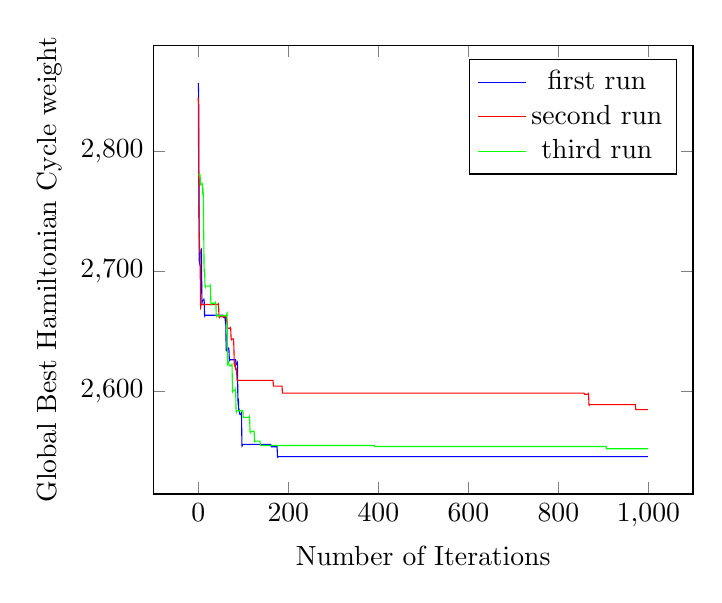
\begin{tikzpicture}
\begin{axis}[
    xlabel={Number of Iterations},
    ylabel={Global Best Hamiltonian Cycle weight},
    legend pos=north east,
    smooth
]
 
\addplot[
    color=blue,smooth
    ]
    coordinates {
    (0,2856.61711040324)(1,2834.4963736237473)(2,2715.4757208435844)(3,2715.4757208435844)(4,2715.4757208435844)(5,2715.4757208435844)(6,2715.4757208435844)(7,2715.4757208435844)(8,2676.029351741456)(9,2676.029351741456)(10,2676.0028690101685)(11,2676.0028690101685)(12,2676.0028690101685)(13,2676.0028690101685)(14,2663.618341609029)(15,2663.618341609029)(16,2663.618341609029)(17,2663.618341609029)(18,2663.618341609029)(19,2663.618341609029)(20,2663.618341609029)(21,2663.618341609029)(22,2663.618341609029)(23,2663.618341609029)(24,2663.618341609029)(25,2663.618341609029)(26,2663.618341609029)(27,2663.618341609029)(28,2663.618341609029)(29,2663.618341609029)(30,2663.618341609029)(31,2663.618341609029)(32,2663.618341609029)(33,2663.618341609029)(34,2663.618341609029)(35,2663.618341609029)(36,2663.618341609029)(37,2663.618341609029)(38,2663.618341609029)(39,2663.618341609029)(40,2663.618341609029)(41,2663.618341609029)(42,2663.618341609029)(43,2663.618341609029)(44,2663.618341609029)(45,2663.618341609029)(46,2663.618341609029)(47,2663.618341609029)(48,2663.618341609029)(49,2663.618341609029)(50,2663.618341609029)(51,2663.618341609029)(52,2663.618341609029)(53,2663.618341609029)(54,2663.618341609029)(55,2663.618341609029)(56,2661.793571283716)(57,2661.793571283716)(58,2661.793571283716)(59,2661.793571283716)(60,2659.0704046575734)(61,2659.0704046575734)(62,2635.5433152462265)(63,2635.5433152462265)(64,2635.5433152462265)(65,2635.5433152462265)(66,2635.5433152462265)(67,2635.5433152462265)(68,2635.5433152462265)(69,2626.616759923102)(70,2626.616759923102)(71,2626.616759923102)(72,2626.616759923102)(73,2626.616759923102)(74,2626.616759923102)(75,2626.616759923102)(76,2626.616759923102)(77,2626.616759923102)(78,2626.616759923102)(79,2626.616759923102)(80,2626.616759923102)(81,2626.616759923102)(82,2626.616759923102)(83,2626.616759923102)(84,2622.6071747724677)(85,2622.6071747724677)(86,2622.6071747724677)(87,2622.6071747724677)(88,2594.0131768664196)(89,2594.0131768664196)(90,2584.3235103283114)(91,2584.3235103283114)(92,2581.4081497232123)(93,2581.4081497232123)(94,2581.4081497232123)(95,2580.886950305201)(96,2580.886950305201)(97,2556.2235648122064)(98,2556.223564812205)(99,2556.223564812205)(100,2556.223564812205)(101,2556.223564812205)(102,2556.223564812205)(103,2556.223564812205)(104,2556.223564812205)(105,2556.223564812205)(106,2556.223564812205)(107,2556.223564812205)(108,2556.223564812205)(109,2556.223564812205)(110,2556.223564812205)(111,2556.223564812205)(112,2556.223564812205)(113,2556.223564812205)(114,2556.223564812205)(115,2556.223564812205)(116,2556.223564812205)(117,2556.223564812205)(118,2556.223564812205)(119,2556.223564812205)(120,2556.223564812205)(121,2556.223564812205)(122,2556.223564812205)(123,2556.223564812205)(124,2556.223564812205)(125,2556.223564812205)(126,2556.223564812205)(127,2556.223564812205)(128,2556.223564812205)(129,2556.223564812205)(130,2556.223564812205)(131,2556.223564812205)(132,2556.223564812205)(133,2556.223564812205)(134,2556.223564812205)(135,2556.223564812205)(136,2556.223564812205)(137,2556.223564812205)(138,2556.223564812205)(139,2556.223564812205)(140,2556.223564812205)(141,2556.223564812205)(142,2556.223564812205)(143,2556.223564812205)(144,2556.223564812205)(145,2556.223564812205)(146,2556.223564812205)(147,2556.223564812205)(148,2556.223564812205)(149,2556.223564812205)(150,2556.223564812205)(151,2556.2235648122046)(152,2556.2235648122046)(153,2556.2235648122046)(154,2556.2235648122046)(155,2556.2235648122046)(156,2556.2235648122046)(157,2556.2235648122046)(158,2556.2235648122046)(159,2556.2235648122046)(160,2556.2235648122046)(161,2556.2235648122046)(162,2554.3280923329603)(163,2554.3280923329603)(164,2554.3280923329603)(165,2554.3280923329603)(166,2554.3280923329603)(167,2554.3280923329603)(168,2554.3280923329603)(169,2554.3280923329603)(170,2554.3280923329603)(171,2554.3280923329603)(172,2554.3280923329603)(173,2554.3280923329603)(174,2554.3280923329603)(175,2554.3280923329603)(176,2546.103340814014)(177,2546.103340814013)(178,2546.103340814013)(179,2546.103340814013)(180,2546.103340814013)(181,2546.103340814013)(182,2546.103340814013)(183,2546.103340814013)(184,2546.103340814013)(185,2546.1033408140124)(186,2546.1033408140124)(187,2546.1033408140124)(188,2546.1033408140124)(189,2546.103340814012)(190,2546.103340814012)(191,2546.103340814012)(192,2546.103340814012)(193,2546.103340814012)(194,2546.103340814012)(195,2546.103340814012)(196,2546.103340814012)(197,2546.103340814012)(198,2546.103340814012)(199,2546.103340814012)(200,2546.103340814012)(201,2546.103340814012)(202,2546.103340814012)(203,2546.103340814012)(204,2546.103340814012)(205,2546.103340814012)(206,2546.103340814012)(207,2546.103340814012)(208,2546.103340814012)(209,2546.103340814012)(210,2546.103340814012)(211,2546.103340814012)(212,2546.103340814012)(213,2546.103340814012)(214,2546.103340814012)(215,2546.103340814012)(216,2546.103340814012)(217,2546.103340814012)(218,2546.103340814012)(219,2546.103340814012)(220,2546.103340814012)(221,2546.103340814012)(222,2546.103340814012)(223,2546.103340814012)(224,2546.103340814012)(225,2546.103340814012)(226,2546.103340814012)(227,2546.103340814012)(228,2546.103340814012)(229,2546.103340814012)(230,2546.103340814012)(231,2546.103340814012)(232,2546.103340814012)(233,2546.103340814012)(234,2546.103340814012)(235,2546.103340814012)(236,2546.103340814012)(237,2546.103340814012)(238,2546.103340814012)(239,2546.103340814012)(240,2546.103340814012)(241,2546.103340814012)(242,2546.103340814012)(243,2546.103340814012)(244,2546.103340814012)(245,2546.103340814012)(246,2546.103340814012)(247,2546.103340814012)(248,2546.103340814012)(249,2546.103340814012)(250,2546.103340814012)(251,2546.103340814012)(252,2546.103340814012)(253,2546.103340814012)(254,2546.103340814012)(255,2546.103340814012)(256,2546.103340814012)(257,2546.103340814012)(258,2546.103340814012)(259,2546.103340814012)(260,2546.103340814012)(261,2546.103340814012)(262,2546.103340814012)(263,2546.103340814012)(264,2546.103340814012)(265,2546.103340814012)(266,2546.103340814012)(267,2546.103340814012)(268,2546.103340814012)(269,2546.103340814012)(270,2546.103340814012)(271,2546.103340814012)(272,2546.103340814012)(273,2546.103340814012)(274,2546.103340814012)(275,2546.103340814012)(276,2546.103340814012)(277,2546.103340814012)(278,2546.103340814012)(279,2546.103340814012)(280,2546.103340814012)(281,2546.103340814012)(282,2546.103340814012)(283,2546.103340814012)(284,2546.103340814012)(285,2546.103340814012)(286,2546.1033408140115)(287,2546.1033408140115)(288,2546.1033408140115)(289,2546.1033408140115)(290,2546.1033408140115)(291,2546.1033408140115)(292,2546.1033408140115)(293,2546.1033408140115)(294,2546.1033408140115)(295,2546.1033408140115)(296,2546.1033408140115)(297,2546.1033408140115)(298,2546.1033408140115)(299,2546.1033408140115)(300,2546.1033408140115)(301,2546.1033408140115)(302,2546.1033408140115)(303,2546.1033408140115)(304,2546.1033408140115)(305,2546.1033408140115)(306,2546.1033408140115)(307,2546.1033408140115)(308,2546.1033408140115)(309,2546.1033408140115)(310,2546.1033408140115)(311,2546.1033408140115)(312,2546.1033408140115)(313,2546.1033408140115)(314,2546.1033408140115)(315,2546.1033408140115)(316,2546.1033408140115)(317,2546.1033408140115)(318,2546.1033408140115)(319,2546.1033408140115)(320,2546.1033408140115)(321,2546.1033408140115)(322,2546.1033408140115)(323,2546.1033408140115)(324,2546.1033408140115)(325,2546.1033408140115)(326,2546.1033408140115)(327,2546.1033408140115)(328,2546.1033408140115)(329,2546.1033408140115)(330,2546.1033408140115)(331,2546.1033408140115)(332,2546.1033408140115)(333,2546.1033408140115)(334,2546.1033408140115)(335,2546.1033408140115)(336,2546.1033408140115)(337,2546.1033408140115)(338,2546.1033408140115)(339,2546.1033408140115)(340,2546.1033408140115)(341,2546.1033408140115)(342,2546.1033408140115)(343,2546.1033408140115)(344,2546.1033408140115)(345,2546.1033408140115)(346,2546.1033408140115)(347,2546.1033408140115)(348,2546.1033408140115)(349,2546.1033408140115)(350,2546.1033408140115)(351,2546.1033408140115)(352,2546.1033408140115)(353,2546.1033408140115)(354,2546.1033408140115)(355,2546.1033408140115)(356,2546.1033408140115)(357,2546.1033408140115)(358,2546.1033408140115)(359,2546.1033408140115)(360,2546.1033408140115)(361,2546.1033408140115)(362,2546.1033408140115)(363,2546.1033408140115)(364,2546.1033408140115)(365,2546.1033408140115)(366,2546.1033408140115)(367,2546.1033408140115)(368,2546.1033408140115)(369,2546.1033408140115)(370,2546.1033408140115)(371,2546.1033408140115)(372,2546.1033408140115)(373,2546.1033408140115)(374,2546.1033408140115)(375,2546.1033408140115)(376,2546.1033408140115)(377,2546.1033408140115)(378,2546.1033408140115)(379,2546.1033408140115)(380,2546.1033408140115)(381,2546.1033408140115)(382,2546.1033408140115)(383,2546.1033408140115)(384,2546.1033408140115)(385,2546.1033408140115)(386,2546.1033408140115)(387,2546.1033408140115)(388,2546.1033408140115)(389,2546.1033408140115)(390,2546.1033408140115)(391,2546.1033408140115)(392,2546.1033408140115)(393,2546.1033408140115)(394,2546.1033408140115)(395,2546.1033408140115)(396,2546.1033408140115)(397,2546.1033408140115)(398,2546.1033408140115)(399,2546.1033408140115)(400,2546.1033408140115)(401,2546.1033408140115)(402,2546.1033408140115)(403,2546.1033408140115)(404,2546.1033408140115)(405,2546.1033408140115)(406,2546.1033408140115)(407,2546.1033408140115)(408,2546.1033408140115)(409,2546.1033408140115)(410,2546.1033408140115)(411,2546.1033408140115)(412,2546.1033408140115)(413,2546.1033408140115)(414,2546.1033408140115)(415,2546.1033408140115)(416,2546.1033408140115)(417,2546.1033408140115)(418,2546.1033408140115)(419,2546.1033408140115)(420,2546.1033408140115)(421,2546.1033408140115)(422,2546.1033408140115)(423,2546.1033408140115)(424,2546.1033408140115)(425,2546.1033408140115)(426,2546.1033408140115)(427,2546.1033408140115)(428,2546.1033408140115)(429,2546.1033408140115)(430,2546.1033408140115)(431,2546.1033408140115)(432,2546.1033408140115)(433,2546.1033408140115)(434,2546.1033408140115)(435,2546.1033408140115)(436,2546.1033408140115)(437,2546.1033408140115)(438,2546.1033408140115)(439,2546.1033408140115)(440,2546.1033408140115)(441,2546.1033408140115)(442,2546.1033408140115)(443,2546.1033408140115)(444,2546.1033408140115)(445,2546.1033408140115)(446,2546.1033408140115)(447,2546.1033408140115)(448,2546.1033408140115)(449,2546.1033408140115)(450,2546.1033408140115)(451,2546.1033408140115)(452,2546.1033408140115)(453,2546.1033408140115)(454,2546.1033408140115)(455,2546.1033408140115)(456,2546.1033408140115)(457,2546.1033408140115)(458,2546.1033408140115)(459,2546.1033408140115)(460,2546.1033408140115)(461,2546.1033408140115)(462,2546.1033408140115)(463,2546.1033408140115)(464,2546.1033408140115)(465,2546.1033408140115)(466,2546.1033408140115)(467,2546.1033408140115)(468,2546.1033408140115)(469,2546.1033408140115)(470,2546.1033408140115)(471,2546.1033408140115)(472,2546.1033408140115)(473,2546.1033408140115)(474,2546.1033408140115)(475,2546.1033408140115)(476,2546.1033408140115)(477,2546.1033408140115)(478,2546.1033408140115)(479,2546.1033408140115)(480,2546.1033408140115)(481,2546.1033408140115)(482,2546.1033408140115)(483,2546.1033408140115)(484,2546.1033408140115)(485,2546.1033408140115)(486,2546.1033408140115)(487,2546.1033408140115)(488,2546.1033408140115)(489,2546.1033408140115)(490,2546.1033408140115)(491,2546.1033408140115)(492,2546.1033408140115)(493,2546.1033408140115)(494,2546.1033408140115)(495,2546.1033408140115)(496,2546.1033408140115)(497,2546.1033408140115)(498,2546.1033408140115)(499,2546.1033408140115)(500,2546.1033408140115)(501,2546.1033408140115)(502,2546.1033408140115)(503,2546.1033408140115)(504,2546.1033408140115)(505,2546.1033408140115)(506,2546.1033408140115)(507,2546.1033408140115)(508,2546.1033408140115)(509,2546.1033408140115)(510,2546.1033408140115)(511,2546.1033408140115)(512,2546.1033408140115)(513,2546.1033408140115)(514,2546.1033408140115)(515,2546.1033408140115)(516,2546.1033408140115)(517,2546.1033408140115)(518,2546.1033408140115)(519,2546.1033408140115)(520,2546.1033408140115)(521,2546.1033408140115)(522,2546.1033408140115)(523,2546.1033408140115)(524,2546.1033408140115)(525,2546.1033408140115)(526,2546.1033408140115)(527,2546.1033408140115)(528,2546.1033408140115)(529,2546.1033408140115)(530,2546.1033408140115)(531,2546.1033408140115)(532,2546.1033408140115)(533,2546.1033408140115)(534,2546.1033408140115)(535,2546.1033408140115)(536,2546.1033408140115)(537,2546.1033408140115)(538,2546.1033408140115)(539,2546.1033408140115)(540,2546.1033408140115)(541,2546.1033408140115)(542,2546.1033408140115)(543,2546.1033408140115)(544,2546.1033408140115)(545,2546.1033408140115)(546,2546.1033408140115)(547,2546.1033408140115)(548,2546.1033408140115)(549,2546.1033408140115)(550,2546.1033408140115)(551,2546.1033408140115)(552,2546.1033408140115)(553,2546.1033408140115)(554,2546.1033408140115)(555,2546.1033408140115)(556,2546.1033408140115)(557,2546.1033408140115)(558,2546.1033408140115)(559,2546.1033408140115)(560,2546.1033408140115)(561,2546.1033408140115)(562,2546.1033408140115)(563,2546.1033408140115)(564,2546.1033408140115)(565,2546.1033408140115)(566,2546.1033408140115)(567,2546.1033408140115)(568,2546.1033408140115)(569,2546.1033408140115)(570,2546.1033408140115)(571,2546.1033408140115)(572,2546.1033408140115)(573,2546.1033408140115)(574,2546.1033408140115)(575,2546.1033408140115)(576,2546.1033408140115)(577,2546.1033408140115)(578,2546.1033408140115)(579,2546.1033408140115)(580,2546.1033408140115)(581,2546.1033408140115)(582,2546.1033408140115)(583,2546.1033408140115)(584,2546.1033408140115)(585,2546.1033408140115)(586,2546.1033408140115)(587,2546.1033408140115)(588,2546.1033408140115)(589,2546.1033408140115)(590,2546.1033408140115)(591,2546.1033408140115)(592,2546.1033408140115)(593,2546.1033408140115)(594,2546.1033408140115)(595,2546.1033408140115)(596,2546.1033408140115)(597,2546.1033408140115)(598,2546.1033408140115)(599,2546.1033408140115)(600,2546.1033408140115)(601,2546.1033408140115)(602,2546.1033408140115)(603,2546.1033408140115)(604,2546.1033408140115)(605,2546.1033408140115)(606,2546.1033408140115)(607,2546.1033408140115)(608,2546.1033408140115)(609,2546.1033408140115)(610,2546.1033408140115)(611,2546.1033408140115)(612,2546.1033408140115)(613,2546.1033408140115)(614,2546.1033408140115)(615,2546.1033408140115)(616,2546.1033408140115)(617,2546.1033408140115)(618,2546.1033408140115)(619,2546.1033408140115)(620,2546.1033408140115)(621,2546.1033408140115)(622,2546.1033408140115)(623,2546.1033408140115)(624,2546.1033408140115)(625,2546.1033408140115)(626,2546.1033408140115)(627,2546.1033408140115)(628,2546.1033408140115)(629,2546.1033408140115)(630,2546.1033408140115)(631,2546.1033408140115)(632,2546.1033408140115)(633,2546.1033408140115)(634,2546.1033408140115)(635,2546.1033408140115)(636,2546.1033408140115)(637,2546.1033408140115)(638,2546.1033408140115)(639,2546.1033408140115)(640,2546.1033408140115)(641,2546.1033408140115)(642,2546.1033408140115)(643,2546.1033408140115)(644,2546.1033408140115)(645,2546.1033408140115)(646,2546.1033408140115)(647,2546.1033408140115)(648,2546.1033408140115)(649,2546.1033408140115)(650,2546.1033408140115)(651,2546.1033408140115)(652,2546.1033408140115)(653,2546.1033408140115)(654,2546.1033408140115)(655,2546.1033408140115)(656,2546.1033408140115)(657,2546.1033408140115)(658,2546.1033408140115)(659,2546.1033408140115)(660,2546.1033408140115)(661,2546.1033408140115)(662,2546.1033408140115)(663,2546.1033408140115)(664,2546.1033408140115)(665,2546.1033408140115)(666,2546.1033408140115)(667,2546.1033408140115)(668,2546.1033408140115)(669,2546.1033408140115)(670,2546.1033408140115)(671,2546.1033408140115)(672,2546.1033408140115)(673,2546.1033408140115)(674,2546.1033408140115)(675,2546.1033408140115)(676,2546.1033408140115)(677,2546.1033408140115)(678,2546.1033408140115)(679,2546.1033408140115)(680,2546.1033408140115)(681,2546.1033408140115)(682,2546.1033408140115)(683,2546.1033408140115)(684,2546.1033408140115)(685,2546.1033408140115)(686,2546.1033408140115)(687,2546.1033408140115)(688,2546.1033408140115)(689,2546.1033408140115)(690,2546.1033408140115)(691,2546.1033408140115)(692,2546.1033408140115)(693,2546.1033408140115)(694,2546.1033408140115)(695,2546.1033408140115)(696,2546.1033408140115)(697,2546.1033408140115)(698,2546.1033408140115)(699,2546.1033408140115)(700,2546.1033408140115)(701,2546.1033408140115)(702,2546.1033408140115)(703,2546.1033408140115)(704,2546.1033408140115)(705,2546.1033408140115)(706,2546.1033408140115)(707,2546.1033408140115)(708,2546.1033408140115)(709,2546.1033408140115)(710,2546.1033408140115)(711,2546.1033408140115)(712,2546.1033408140115)(713,2546.1033408140115)(714,2546.1033408140115)(715,2546.1033408140115)(716,2546.1033408140115)(717,2546.1033408140115)(718,2546.1033408140115)(719,2546.1033408140115)(720,2546.1033408140115)(721,2546.1033408140115)(722,2546.1033408140115)(723,2546.1033408140115)(724,2546.1033408140115)(725,2546.1033408140115)(726,2546.1033408140115)(727,2546.1033408140115)(728,2546.1033408140115)(729,2546.1033408140115)(730,2546.1033408140115)(731,2546.1033408140115)(732,2546.1033408140115)(733,2546.1033408140115)(734,2546.1033408140115)(735,2546.1033408140115)(736,2546.1033408140115)(737,2546.1033408140115)(738,2546.1033408140115)(739,2546.1033408140115)(740,2546.1033408140115)(741,2546.1033408140115)(742,2546.1033408140115)(743,2546.1033408140115)(744,2546.1033408140115)(745,2546.1033408140115)(746,2546.1033408140115)(747,2546.1033408140115)(748,2546.1033408140115)(749,2546.1033408140115)(750,2546.1033408140115)(751,2546.1033408140115)(752,2546.1033408140115)(753,2546.1033408140115)(754,2546.1033408140115)(755,2546.1033408140115)(756,2546.1033408140115)(757,2546.1033408140115)(758,2546.1033408140115)(759,2546.1033408140115)(760,2546.1033408140115)(761,2546.1033408140115)(762,2546.1033408140115)(763,2546.1033408140115)(764,2546.1033408140115)(765,2546.1033408140115)(766,2546.1033408140115)(767,2546.1033408140115)(768,2546.1033408140115)(769,2546.1033408140115)(770,2546.1033408140115)(771,2546.1033408140115)(772,2546.1033408140115)(773,2546.1033408140115)(774,2546.1033408140115)(775,2546.1033408140115)(776,2546.1033408140115)(777,2546.1033408140115)(778,2546.1033408140115)(779,2546.1033408140115)(780,2546.1033408140115)(781,2546.1033408140115)(782,2546.1033408140115)(783,2546.1033408140115)(784,2546.1033408140115)(785,2546.1033408140115)(786,2546.1033408140115)(787,2546.1033408140115)(788,2546.1033408140115)(789,2546.1033408140115)(790,2546.1033408140115)(791,2546.1033408140115)(792,2546.1033408140115)(793,2546.1033408140115)(794,2546.1033408140115)(795,2546.1033408140115)(796,2546.1033408140115)(797,2546.1033408140115)(798,2546.1033408140115)(799,2546.1033408140115)(800,2546.1033408140115)(801,2546.1033408140115)(802,2546.1033408140115)(803,2546.1033408140115)(804,2546.1033408140115)(805,2546.1033408140115)(806,2546.1033408140115)(807,2546.1033408140115)(808,2546.1033408140115)(809,2546.1033408140115)(810,2546.1033408140115)(811,2546.1033408140115)(812,2546.1033408140115)(813,2546.1033408140115)(814,2546.1033408140115)(815,2546.1033408140115)(816,2546.1033408140115)(817,2546.1033408140115)(818,2546.1033408140115)(819,2546.1033408140115)(820,2546.1033408140115)(821,2546.1033408140115)(822,2546.1033408140115)(823,2546.1033408140115)(824,2546.1033408140115)(825,2546.1033408140115)(826,2546.1033408140115)(827,2546.1033408140115)(828,2546.1033408140115)(829,2546.1033408140115)(830,2546.1033408140115)(831,2546.1033408140115)(832,2546.1033408140115)(833,2546.1033408140115)(834,2546.1033408140115)(835,2546.1033408140115)(836,2546.1033408140115)(837,2546.1033408140115)(838,2546.1033408140115)(839,2546.1033408140115)(840,2546.1033408140115)(841,2546.1033408140115)(842,2546.1033408140115)(843,2546.1033408140115)(844,2546.1033408140115)(845,2546.1033408140115)(846,2546.1033408140115)(847,2546.1033408140115)(848,2546.1033408140115)(849,2546.1033408140115)(850,2546.1033408140115)(851,2546.1033408140115)(852,2546.1033408140115)(853,2546.1033408140115)(854,2546.1033408140115)(855,2546.1033408140115)(856,2546.1033408140115)(857,2546.1033408140115)(858,2546.1033408140115)(859,2546.1033408140115)(860,2546.1033408140115)(861,2546.1033408140115)(862,2546.1033408140115)(863,2546.1033408140115)(864,2546.1033408140115)(865,2546.1033408140115)(866,2546.1033408140115)(867,2546.1033408140115)(868,2546.1033408140115)(869,2546.1033408140115)(870,2546.1033408140115)(871,2546.1033408140115)(872,2546.1033408140115)(873,2546.1033408140115)(874,2546.1033408140115)(875,2546.1033408140115)(876,2546.1033408140115)(877,2546.1033408140115)(878,2546.1033408140115)(879,2546.1033408140115)(880,2546.1033408140115)(881,2546.1033408140115)(882,2546.1033408140115)(883,2546.1033408140115)(884,2546.1033408140115)(885,2546.1033408140115)(886,2546.1033408140115)(887,2546.1033408140115)(888,2546.1033408140115)(889,2546.1033408140115)(890,2546.1033408140115)(891,2546.1033408140115)(892,2546.1033408140115)(893,2546.1033408140115)(894,2546.1033408140115)(895,2546.1033408140115)(896,2546.1033408140115)(897,2546.1033408140115)(898,2546.1033408140115)(899,2546.1033408140115)(900,2546.1033408140115)(901,2546.1033408140115)(902,2546.1033408140115)(903,2546.1033408140115)(904,2546.1033408140115)(905,2546.1033408140115)(906,2546.1033408140115)(907,2546.1033408140115)(908,2546.1033408140115)(909,2546.1033408140115)(910,2546.1033408140115)(911,2546.1033408140115)(912,2546.1033408140115)(913,2546.1033408140115)(914,2546.1033408140115)(915,2546.1033408140115)(916,2546.1033408140115)(917,2546.1033408140115)(918,2546.1033408140115)(919,2546.1033408140115)(920,2546.1033408140115)(921,2546.1033408140115)(922,2546.1033408140115)(923,2546.1033408140115)(924,2546.1033408140115)(925,2546.1033408140115)(926,2546.1033408140115)(927,2546.1033408140115)(928,2546.1033408140115)(929,2546.1033408140115)(930,2546.1033408140115)(931,2546.1033408140115)(932,2546.1033408140115)(933,2546.1033408140115)(934,2546.1033408140115)(935,2546.1033408140115)(936,2546.1033408140115)(937,2546.1033408140115)(938,2546.1033408140115)(939,2546.1033408140115)(940,2546.1033408140115)(941,2546.1033408140115)(942,2546.1033408140115)(943,2546.1033408140115)(944,2546.1033408140115)(945,2546.1033408140115)(946,2546.1033408140115)(947,2546.1033408140115)(948,2546.1033408140115)(949,2546.1033408140115)(950,2546.1033408140115)(951,2546.1033408140115)(952,2546.1033408140115)(953,2546.1033408140115)(954,2546.1033408140115)(955,2546.1033408140115)(956,2546.1033408140115)(957,2546.1033408140115)(958,2546.1033408140115)(959,2546.1033408140115)(960,2546.1033408140115)(961,2546.1033408140115)(962,2546.1033408140115)(963,2546.1033408140115)(964,2546.1033408140115)(965,2546.1033408140115)(966,2546.1033408140115)(967,2546.1033408140115)(968,2546.1033408140115)(969,2546.1033408140115)(970,2546.1033408140115)(971,2546.1033408140115)(972,2546.1033408140115)(973,2546.1033408140115)(974,2546.1033408140115)(975,2546.1033408140115)(976,2546.1033408140115)(977,2546.1033408140115)(978,2546.1033408140115)(979,2546.1033408140115)(980,2546.1033408140115)(981,2546.1033408140115)(982,2546.1033408140115)(983,2546.1033408140115)(984,2546.1033408140115)(985,2546.1033408140115)(986,2546.1033408140115)(987,2546.1033408140115)(988,2546.1033408140115)(989,2546.1033408140115)(990,2546.1033408140115)(991,2546.1033408140115)(992,2546.1033408140115)(993,2546.1033408140115)(994,2546.1033408140115)(995,2546.1033408140115)(996,2546.1033408140115)(997,2546.1033408140115)(998,2546.1033408140115)(999,2546.1033408140115)
    };
   \addlegendentry{first run}
\addplot[
    color=red,smooth
    ]
    coordinates {
    (0,2844.4316858423276)(1,2778.274501695867)(2,2733.571118388988)(3,2718.6664583322427)(4,2714.8947212388125)(5,2672.480805827865)(6,2672.480805827865)(7,2672.480805827865)(8,2672.480805827865)(9,2672.480805827865)(10,2672.480805827865)(11,2672.480805827865)(12,2672.4808058278622)(13,2672.4808058278622)(14,2672.4808058278622)(15,2672.4808058278622)(16,2672.4808058278622)(17,2672.4808058278622)(18,2672.4808058278622)(19,2672.4808058278622)(20,2672.4808058278622)(21,2672.4808058278622)(22,2672.4808058278622)(23,2672.4808058278622)(24,2672.4808058278622)(25,2672.4808058278622)(26,2672.4808058278622)(27,2672.4808058278622)(28,2672.4808058278622)(29,2672.4808058278622)(30,2672.4808058278622)(31,2672.4808058278622)(32,2672.4808058278622)(33,2672.4808058278622)(34,2672.4808058278622)(35,2672.4808058278622)(36,2672.4808058278622)(37,2672.4808058278622)(38,2672.4808058278622)(39,2672.4808058278622)(40,2672.4808058278622)(41,2672.4808058278622)(42,2672.4808058278622)(43,2672.4808058278622)(44,2672.4808058278622)(45,2672.4808058278622)(46,2662.3375095568886)(47,2662.337509556887)(48,2662.337509556887)(49,2662.337509556887)(50,2662.337509556887)(51,2662.337509556887)(52,2662.337509556887)(53,2662.337509556887)(54,2662.337509556887)(55,2662.337509556887)(56,2662.337509556887)(57,2662.337509556887)(58,2662.337509556887)(59,2662.337509556887)(60,2662.337509556887)(61,2662.337509556887)(62,2662.337509556887)(63,2658.798667763867)(64,2658.798667763867)(65,2652.7390420568795)(66,2652.7390420568795)(67,2652.7390420568795)(68,2652.7390420568795)(69,2652.7390420568795)(70,2652.7390420568795)(71,2652.7390420568795)(72,2652.7390420568795)(73,2643.8382617808065)(74,2643.8382617808065)(75,2643.8382617808065)(76,2643.8382617808065)(77,2643.8382617808065)(78,2643.838261780806)(79,2637.89164077379)(80,2623.052792521236)(81,2623.052792521236)(82,2623.0527925212346)(83,2618.424387216354)(84,2618.424387216354)(85,2618.424387216354)(86,2610.292805234605)(87,2609.4263120544188)(88,2609.4263120544188)(89,2609.4263120544188)(90,2609.4263120544183)(91,2609.4263120544183)(92,2609.4263120544183)(93,2609.4263120544174)(94,2609.4263120544174)(95,2609.4263120544174)(96,2609.4263120544174)(97,2609.4263120544174)(98,2609.4263120544174)(99,2609.4263120544174)(100,2609.4263120544174)(101,2609.4263120544174)(102,2609.4263120544174)(103,2609.4263120544174)(104,2609.4263120544174)(105,2609.4263120544174)(106,2609.4263120544174)(107,2609.4263120544174)(108,2609.4263120544174)(109,2609.4263120544174)(110,2609.4263120544174)(111,2609.4263120544174)(112,2609.4263120544174)(113,2609.4263120544174)(114,2609.4263120544174)(115,2609.4263120544174)(116,2609.4263120544174)(117,2609.4263120544174)(118,2609.4263120544174)(119,2609.4263120544174)(120,2609.4263120544174)(121,2609.4263120544174)(122,2609.4263120544174)(123,2609.4263120544174)(124,2609.4263120544174)(125,2609.4263120544174)(126,2609.4263120544174)(127,2609.4263120544174)(128,2609.4263120544174)(129,2609.4263120544174)(130,2609.4263120544174)(131,2609.4263120544174)(132,2609.4263120544174)(133,2609.4263120544174)(134,2609.4263120544174)(135,2609.4263120544174)(136,2609.4263120544174)(137,2609.4263120544174)(138,2609.4263120544174)(139,2609.4263120544174)(140,2609.4263120544174)(141,2609.4263120544174)(142,2609.4263120544174)(143,2609.4263120544174)(144,2609.4263120544174)(145,2609.4263120544174)(146,2609.4263120544174)(147,2609.4263120544174)(148,2609.4263120544174)(149,2609.4263120544174)(150,2609.4263120544174)(151,2609.4263120544174)(152,2609.4263120544174)(153,2609.4263120544174)(154,2609.4263120544174)(155,2609.4263120544174)(156,2609.4263120544174)(157,2609.4263120544174)(158,2609.4263120544174)(159,2609.4263120544174)(160,2609.4263120544174)(161,2609.4263120544174)(162,2609.4263120544174)(163,2609.4263120544174)(164,2609.4263120544174)(165,2609.4263120544174)(166,2609.4263120544174)(167,2604.69260664025)(168,2604.69260664025)(169,2604.69260664025)(170,2604.69260664025)(171,2604.69260664025)(172,2604.69260664025)(173,2604.69260664025)(174,2604.69260664025)(175,2604.69260664025)(176,2604.69260664025)(177,2604.69260664025)(178,2604.69260664025)(179,2604.69260664025)(180,2604.69260664025)(181,2604.69260664025)(182,2604.69260664025)(183,2604.69260664025)(184,2604.69260664025)(185,2604.69260664025)(186,2604.69260664025)(187,2598.8027752178377)(188,2598.8027752178377)(189,2598.8027752178377)(190,2598.8027752178377)(191,2598.8027752178377)(192,2598.8027752178377)(193,2598.8027752178377)(194,2598.8027752178377)(195,2598.8027752178377)(196,2598.8027752178377)(197,2598.8027752178377)(198,2598.8027752178377)(199,2598.8027752178373)(200,2598.8027752178373)(201,2598.8027752178373)(202,2598.8027752178373)(203,2598.8027752178373)(204,2598.8027752178373)(205,2598.802775217837)(206,2598.802775217837)(207,2598.802775217837)(208,2598.802775217837)(209,2598.802775217837)(210,2598.802775217837)(211,2598.802775217837)(212,2598.802775217837)(213,2598.802775217837)(214,2598.802775217837)(215,2598.802775217837)(216,2598.802775217837)(217,2598.802775217837)(218,2598.802775217837)(219,2598.802775217837)(220,2598.802775217837)(221,2598.802775217837)(222,2598.802775217837)(223,2598.802775217837)(224,2598.802775217837)(225,2598.802775217837)(226,2598.802775217837)(227,2598.802775217837)(228,2598.802775217837)(229,2598.802775217837)(230,2598.802775217837)(231,2598.802775217837)(232,2598.802775217837)(233,2598.802775217837)(234,2598.802775217837)(235,2598.802775217837)(236,2598.802775217837)(237,2598.802775217837)(238,2598.802775217837)(239,2598.802775217837)(240,2598.802775217837)(241,2598.802775217837)(242,2598.802775217837)(243,2598.802775217837)(244,2598.802775217837)(245,2598.802775217837)(246,2598.802775217837)(247,2598.802775217837)(248,2598.802775217837)(249,2598.802775217837)(250,2598.802775217837)(251,2598.802775217837)(252,2598.802775217837)(253,2598.802775217837)(254,2598.802775217837)(255,2598.802775217837)(256,2598.802775217837)(257,2598.802775217837)(258,2598.802775217837)(259,2598.802775217837)(260,2598.802775217837)(261,2598.802775217837)(262,2598.802775217837)(263,2598.802775217837)(264,2598.802775217837)(265,2598.802775217837)(266,2598.802775217837)(267,2598.802775217837)(268,2598.802775217837)(269,2598.802775217837)(270,2598.802775217837)(271,2598.802775217837)(272,2598.802775217837)(273,2598.802775217837)(274,2598.802775217837)(275,2598.802775217837)(276,2598.802775217837)(277,2598.802775217837)(278,2598.802775217837)(279,2598.802775217837)(280,2598.802775217837)(281,2598.802775217837)(282,2598.802775217837)(283,2598.802775217837)(284,2598.802775217837)(285,2598.802775217837)(286,2598.802775217837)(287,2598.802775217837)(288,2598.802775217837)(289,2598.802775217837)(290,2598.802775217837)(291,2598.802775217837)(292,2598.802775217837)(293,2598.802775217837)(294,2598.802775217837)(295,2598.802775217837)(296,2598.802775217837)(297,2598.802775217837)(298,2598.802775217837)(299,2598.802775217837)(300,2598.802775217837)(301,2598.802775217837)(302,2598.802775217837)(303,2598.802775217837)(304,2598.802775217837)(305,2598.802775217837)(306,2598.802775217837)(307,2598.802775217837)(308,2598.802775217837)(309,2598.802775217837)(310,2598.802775217837)(311,2598.802775217837)(312,2598.802775217837)(313,2598.802775217837)(314,2598.802775217837)(315,2598.802775217837)(316,2598.802775217837)(317,2598.802775217837)(318,2598.802775217837)(319,2598.802775217837)(320,2598.802775217837)(321,2598.802775217837)(322,2598.802775217837)(323,2598.802775217837)(324,2598.802775217837)(325,2598.802775217837)(326,2598.802775217837)(327,2598.802775217837)(328,2598.802775217837)(329,2598.802775217837)(330,2598.802775217837)(331,2598.802775217837)(332,2598.802775217837)(333,2598.802775217837)(334,2598.802775217837)(335,2598.802775217837)(336,2598.802775217837)(337,2598.802775217837)(338,2598.802775217837)(339,2598.802775217837)(340,2598.802775217837)(341,2598.802775217837)(342,2598.802775217837)(343,2598.802775217837)(344,2598.802775217837)(345,2598.802775217837)(346,2598.802775217837)(347,2598.802775217837)(348,2598.802775217837)(349,2598.802775217837)(350,2598.802775217837)(351,2598.802775217837)(352,2598.802775217837)(353,2598.802775217837)(354,2598.802775217837)(355,2598.802775217837)(356,2598.802775217837)(357,2598.802775217837)(358,2598.802775217837)(359,2598.802775217837)(360,2598.802775217837)(361,2598.802775217837)(362,2598.802775217837)(363,2598.802775217837)(364,2598.802775217837)(365,2598.802775217837)(366,2598.802775217837)(367,2598.802775217837)(368,2598.802775217837)(369,2598.802775217837)(370,2598.802775217837)(371,2598.802775217837)(372,2598.802775217837)(373,2598.802775217837)(374,2598.802775217837)(375,2598.802775217837)(376,2598.802775217837)(377,2598.802775217837)(378,2598.802775217837)(379,2598.802775217837)(380,2598.802775217837)(381,2598.802775217837)(382,2598.802775217837)(383,2598.802775217837)(384,2598.802775217837)(385,2598.802775217837)(386,2598.802775217837)(387,2598.802775217837)(388,2598.802775217837)(389,2598.802775217837)(390,2598.802775217837)(391,2598.802775217837)(392,2598.802775217837)(393,2598.802775217837)(394,2598.802775217837)(395,2598.802775217837)(396,2598.802775217837)(397,2598.802775217837)(398,2598.802775217837)(399,2598.802775217837)(400,2598.802775217837)(401,2598.802775217837)(402,2598.802775217837)(403,2598.802775217837)(404,2598.802775217837)(405,2598.802775217837)(406,2598.802775217837)(407,2598.802775217837)(408,2598.802775217837)(409,2598.802775217837)(410,2598.802775217837)(411,2598.802775217837)(412,2598.802775217837)(413,2598.802775217837)(414,2598.802775217837)(415,2598.802775217837)(416,2598.802775217837)(417,2598.802775217837)(418,2598.802775217837)(419,2598.802775217837)(420,2598.802775217837)(421,2598.802775217837)(422,2598.802775217837)(423,2598.802775217837)(424,2598.802775217837)(425,2598.802775217837)(426,2598.802775217837)(427,2598.802775217837)(428,2598.802775217837)(429,2598.802775217837)(430,2598.802775217837)(431,2598.802775217837)(432,2598.802775217837)(433,2598.802775217837)(434,2598.802775217837)(435,2598.802775217837)(436,2598.802775217837)(437,2598.802775217837)(438,2598.802775217837)(439,2598.802775217837)(440,2598.802775217837)(441,2598.802775217837)(442,2598.802775217837)(443,2598.802775217837)(444,2598.802775217837)(445,2598.802775217837)(446,2598.802775217837)(447,2598.802775217837)(448,2598.802775217837)(449,2598.802775217837)(450,2598.802775217837)(451,2598.802775217837)(452,2598.802775217837)(453,2598.802775217837)(454,2598.802775217837)(455,2598.802775217837)(456,2598.802775217837)(457,2598.802775217837)(458,2598.802775217837)(459,2598.802775217837)(460,2598.802775217837)(461,2598.802775217837)(462,2598.802775217837)(463,2598.802775217837)(464,2598.802775217837)(465,2598.802775217837)(466,2598.802775217837)(467,2598.802775217837)(468,2598.802775217837)(469,2598.802775217837)(470,2598.802775217837)(471,2598.802775217837)(472,2598.802775217837)(473,2598.802775217837)(474,2598.802775217837)(475,2598.802775217837)(476,2598.802775217837)(477,2598.802775217837)(478,2598.802775217837)(479,2598.802775217837)(480,2598.802775217837)(481,2598.802775217837)(482,2598.802775217837)(483,2598.802775217837)(484,2598.802775217837)(485,2598.802775217837)(486,2598.802775217837)(487,2598.802775217837)(488,2598.802775217837)(489,2598.802775217837)(490,2598.802775217837)(491,2598.802775217837)(492,2598.802775217837)(493,2598.802775217837)(494,2598.802775217837)(495,2598.802775217837)(496,2598.802775217837)(497,2598.802775217837)(498,2598.802775217837)(499,2598.802775217837)(500,2598.802775217837)(501,2598.802775217837)(502,2598.802775217837)(503,2598.802775217837)(504,2598.802775217837)(505,2598.802775217837)(506,2598.802775217837)(507,2598.802775217837)(508,2598.802775217837)(509,2598.802775217837)(510,2598.802775217837)(511,2598.802775217837)(512,2598.802775217837)(513,2598.802775217837)(514,2598.802775217837)(515,2598.802775217837)(516,2598.802775217837)(517,2598.802775217837)(518,2598.802775217837)(519,2598.802775217837)(520,2598.802775217837)(521,2598.802775217837)(522,2598.802775217837)(523,2598.802775217837)(524,2598.802775217837)(525,2598.802775217837)(526,2598.802775217837)(527,2598.802775217837)(528,2598.802775217837)(529,2598.802775217837)(530,2598.802775217837)(531,2598.802775217837)(532,2598.802775217837)(533,2598.802775217837)(534,2598.802775217837)(535,2598.802775217837)(536,2598.802775217837)(537,2598.802775217837)(538,2598.802775217837)(539,2598.802775217837)(540,2598.802775217837)(541,2598.802775217837)(542,2598.802775217837)(543,2598.802775217837)(544,2598.802775217837)(545,2598.802775217837)(546,2598.802775217837)(547,2598.802775217837)(548,2598.802775217837)(549,2598.802775217837)(550,2598.802775217837)(551,2598.802775217837)(552,2598.802775217837)(553,2598.802775217837)(554,2598.802775217837)(555,2598.802775217837)(556,2598.802775217837)(557,2598.802775217837)(558,2598.802775217837)(559,2598.802775217837)(560,2598.802775217837)(561,2598.802775217837)(562,2598.802775217837)(563,2598.802775217837)(564,2598.802775217837)(565,2598.802775217837)(566,2598.802775217837)(567,2598.802775217837)(568,2598.802775217837)(569,2598.802775217837)(570,2598.802775217837)(571,2598.802775217837)(572,2598.802775217837)(573,2598.802775217837)(574,2598.802775217837)(575,2598.802775217837)(576,2598.802775217837)(577,2598.802775217837)(578,2598.802775217837)(579,2598.802775217837)(580,2598.802775217837)(581,2598.802775217837)(582,2598.802775217837)(583,2598.802775217837)(584,2598.802775217837)(585,2598.802775217837)(586,2598.802775217837)(587,2598.802775217837)(588,2598.802775217837)(589,2598.802775217837)(590,2598.802775217837)(591,2598.802775217837)(592,2598.802775217837)(593,2598.802775217837)(594,2598.802775217837)(595,2598.802775217837)(596,2598.802775217837)(597,2598.802775217837)(598,2598.802775217837)(599,2598.802775217837)(600,2598.802775217837)(601,2598.802775217837)(602,2598.802775217837)(603,2598.802775217837)(604,2598.802775217837)(605,2598.802775217837)(606,2598.802775217837)(607,2598.802775217837)(608,2598.802775217837)(609,2598.802775217837)(610,2598.802775217837)(611,2598.802775217837)(612,2598.802775217837)(613,2598.802775217837)(614,2598.802775217837)(615,2598.802775217837)(616,2598.802775217837)(617,2598.802775217837)(618,2598.802775217837)(619,2598.802775217837)(620,2598.802775217837)(621,2598.802775217837)(622,2598.802775217837)(623,2598.802775217837)(624,2598.802775217837)(625,2598.802775217837)(626,2598.802775217837)(627,2598.802775217837)(628,2598.802775217837)(629,2598.802775217837)(630,2598.802775217837)(631,2598.802775217837)(632,2598.802775217837)(633,2598.802775217837)(634,2598.802775217837)(635,2598.802775217837)(636,2598.802775217837)(637,2598.802775217837)(638,2598.802775217837)(639,2598.802775217837)(640,2598.802775217837)(641,2598.802775217837)(642,2598.802775217837)(643,2598.802775217837)(644,2598.802775217837)(645,2598.802775217837)(646,2598.802775217837)(647,2598.802775217837)(648,2598.802775217837)(649,2598.802775217837)(650,2598.802775217837)(651,2598.802775217837)(652,2598.802775217837)(653,2598.802775217837)(654,2598.802775217837)(655,2598.802775217837)(656,2598.802775217837)(657,2598.802775217837)(658,2598.802775217837)(659,2598.802775217837)(660,2598.802775217837)(661,2598.802775217837)(662,2598.802775217837)(663,2598.802775217837)(664,2598.802775217837)(665,2598.802775217837)(666,2598.802775217837)(667,2598.802775217837)(668,2598.802775217837)(669,2598.802775217837)(670,2598.802775217837)(671,2598.802775217837)(672,2598.802775217837)(673,2598.802775217837)(674,2598.802775217837)(675,2598.802775217837)(676,2598.802775217837)(677,2598.802775217837)(678,2598.802775217837)(679,2598.802775217837)(680,2598.802775217837)(681,2598.802775217837)(682,2598.802775217837)(683,2598.802775217837)(684,2598.802775217837)(685,2598.802775217837)(686,2598.802775217837)(687,2598.802775217837)(688,2598.802775217837)(689,2598.802775217837)(690,2598.802775217837)(691,2598.802775217837)(692,2598.802775217837)(693,2598.802775217837)(694,2598.802775217837)(695,2598.802775217837)(696,2598.802775217837)(697,2598.802775217837)(698,2598.802775217837)(699,2598.802775217837)(700,2598.802775217837)(701,2598.802775217837)(702,2598.802775217837)(703,2598.802775217837)(704,2598.802775217837)(705,2598.802775217837)(706,2598.802775217837)(707,2598.802775217837)(708,2598.802775217837)(709,2598.802775217837)(710,2598.802775217837)(711,2598.802775217837)(712,2598.802775217837)(713,2598.802775217837)(714,2598.802775217837)(715,2598.802775217837)(716,2598.802775217837)(717,2598.802775217837)(718,2598.802775217837)(719,2598.802775217837)(720,2598.802775217837)(721,2598.802775217837)(722,2598.802775217837)(723,2598.802775217837)(724,2598.802775217837)(725,2598.802775217837)(726,2598.802775217837)(727,2598.802775217837)(728,2598.802775217837)(729,2598.802775217837)(730,2598.802775217837)(731,2598.802775217837)(732,2598.802775217837)(733,2598.802775217837)(734,2598.802775217837)(735,2598.802775217837)(736,2598.802775217837)(737,2598.802775217837)(738,2598.802775217837)(739,2598.802775217837)(740,2598.802775217837)(741,2598.802775217837)(742,2598.802775217837)(743,2598.802775217837)(744,2598.802775217837)(745,2598.802775217837)(746,2598.802775217837)(747,2598.802775217837)(748,2598.802775217837)(749,2598.802775217837)(750,2598.802775217837)(751,2598.802775217837)(752,2598.802775217837)(753,2598.802775217837)(754,2598.802775217837)(755,2598.802775217837)(756,2598.802775217837)(757,2598.802775217837)(758,2598.802775217837)(759,2598.802775217837)(760,2598.802775217837)(761,2598.802775217837)(762,2598.802775217837)(763,2598.802775217837)(764,2598.802775217837)(765,2598.802775217837)(766,2598.802775217837)(767,2598.802775217837)(768,2598.802775217837)(769,2598.802775217837)(770,2598.802775217837)(771,2598.802775217837)(772,2598.802775217837)(773,2598.802775217837)(774,2598.802775217837)(775,2598.802775217837)(776,2598.802775217837)(777,2598.802775217837)(778,2598.802775217837)(779,2598.802775217837)(780,2598.802775217837)(781,2598.802775217837)(782,2598.802775217837)(783,2598.802775217837)(784,2598.802775217837)(785,2598.802775217837)(786,2598.802775217837)(787,2598.802775217837)(788,2598.802775217837)(789,2598.802775217837)(790,2598.802775217837)(791,2598.802775217837)(792,2598.802775217837)(793,2598.802775217837)(794,2598.802775217837)(795,2598.802775217837)(796,2598.802775217837)(797,2598.802775217837)(798,2598.802775217837)(799,2598.802775217837)(800,2598.802775217837)(801,2598.802775217837)(802,2598.802775217837)(803,2598.802775217837)(804,2598.802775217837)(805,2598.802775217837)(806,2598.802775217837)(807,2598.802775217837)(808,2598.802775217837)(809,2598.802775217837)(810,2598.802775217837)(811,2598.802775217837)(812,2598.802775217837)(813,2598.802775217837)(814,2598.802775217837)(815,2598.802775217837)(816,2598.802775217837)(817,2598.802775217837)(818,2598.802775217837)(819,2598.802775217837)(820,2598.802775217837)(821,2598.802775217837)(822,2598.802775217837)(823,2598.802775217837)(824,2598.802775217837)(825,2598.802775217837)(826,2598.802775217837)(827,2598.802775217837)(828,2598.802775217837)(829,2598.802775217837)(830,2598.802775217837)(831,2598.802775217837)(832,2598.802775217837)(833,2598.802775217837)(834,2598.802775217837)(835,2598.802775217837)(836,2598.802775217837)(837,2598.802775217837)(838,2598.802775217837)(839,2598.802775217837)(840,2598.802775217837)(841,2598.802775217837)(842,2598.802775217837)(843,2598.802775217837)(844,2598.802775217837)(845,2598.802775217837)(846,2598.802775217837)(847,2598.802775217837)(848,2598.802775217837)(849,2598.802775217837)(850,2598.802775217837)(851,2598.802775217837)(852,2598.802775217837)(853,2598.802775217837)(854,2598.802775217837)(855,2598.802775217837)(856,2598.802775217837)(857,2598.802775217837)(858,2597.913829702717)(859,2597.913829702717)(860,2597.913829702717)(861,2597.913829702717)(862,2597.913829702717)(863,2597.913829702717)(864,2597.913829702717)(865,2597.913829702717)(866,2597.913829702717)(867,2597.913829702717)(868,2589.329353960091)(869,2589.329353960091)(870,2589.329353960091)(871,2589.329353960091)(872,2589.329353960091)(873,2589.329353960091)(874,2589.329353960091)(875,2589.3293539600904)(876,2589.3293539600904)(877,2589.3293539600904)(878,2589.3293539600904)(879,2589.3293539600904)(880,2589.3293539600904)(881,2589.3293539600904)(882,2589.3293539600904)(883,2589.3293539600904)(884,2589.3293539600904)(885,2589.3293539600904)(886,2589.3293539600904)(887,2589.3293539600904)(888,2589.3293539600904)(889,2589.3293539600904)(890,2589.3293539600904)(891,2589.3293539600904)(892,2589.3293539600904)(893,2589.3293539600904)(894,2589.3293539600904)(895,2589.3293539600904)(896,2589.3293539600904)(897,2589.3293539600904)(898,2589.3293539600904)(899,2589.3293539600904)(900,2589.3293539600904)(901,2589.3293539600904)(902,2589.3293539600904)(903,2589.3293539600904)(904,2589.3293539600904)(905,2589.3293539600904)(906,2589.3293539600904)(907,2589.3293539600904)(908,2589.3293539600904)(909,2589.3293539600904)(910,2589.3293539600904)(911,2589.3293539600904)(912,2589.3293539600904)(913,2589.3293539600904)(914,2589.3293539600904)(915,2589.3293539600904)(916,2589.3293539600904)(917,2589.3293539600904)(918,2589.3293539600904)(919,2589.3293539600904)(920,2589.3293539600904)(921,2589.3293539600904)(922,2589.3293539600904)(923,2589.3293539600904)(924,2589.3293539600904)(925,2589.3293539600904)(926,2589.3293539600904)(927,2589.3293539600904)(928,2589.3293539600904)(929,2589.3293539600904)(930,2589.3293539600904)(931,2589.3293539600904)(932,2589.3293539600904)(933,2589.3293539600904)(934,2589.3293539600904)(935,2589.3293539600904)(936,2589.3293539600904)(937,2589.3293539600904)(938,2589.3293539600904)(939,2589.3293539600904)(940,2589.3293539600904)(941,2589.3293539600904)(942,2589.3293539600904)(943,2589.3293539600904)(944,2589.3293539600904)(945,2589.3293539600904)(946,2589.3293539600904)(947,2589.3293539600904)(948,2589.3293539600904)(949,2589.3293539600904)(950,2589.3293539600904)(951,2589.3293539600904)(952,2589.3293539600904)(953,2589.3293539600904)(954,2589.3293539600904)(955,2589.3293539600904)(956,2589.3293539600904)(957,2589.3293539600904)(958,2589.3293539600904)(959,2589.3293539600904)(960,2589.3293539600904)(961,2589.3293539600904)(962,2589.3293539600904)(963,2589.3293539600904)(964,2589.3293539600904)(965,2589.3293539600904)(966,2589.3293539600904)(967,2589.3293539600904)(968,2589.3293539600904)(969,2589.3293539600904)(970,2589.3293539600904)(971,2589.3293539600904)(972,2585.1918911531516)(973,2585.1918911531516)(974,2585.1918911531516)(975,2585.1918911531516)(976,2585.1918911531516)(977,2585.1918911531516)(978,2585.1918911531516)(979,2585.1918911531516)(980,2585.1918911531516)(981,2585.1918911531516)(982,2585.1918911531516)(983,2585.1918911531516)(984,2585.1918911531516)(985,2585.1918911531516)(986,2585.1918911531516)(987,2585.1918911531516)(988,2585.1918911531516)(989,2585.1918911531516)(990,2585.1918911531516)(991,2585.1918911531516)(992,2585.1918911531516)(993,2585.1918911531516)(994,2585.1918911531516)(995,2585.1918911531516)(996,2585.1918911531516)(997,2585.1918911531516)(998,2585.1918911531516)(999,2585.1918911531516)
    };
   \addlegendentry{second run}
\addplot[color=green,smooth]
coordinates{(0,2780.3379864821804)(1,2780.33798648218)(2,2780.337986482179)(3,2780.337986482179)(4,2780.337986482179)(5,2772.598182083272)(6,2772.598182083272)(7,2772.598182083272)(8,2772.598182083272)(9,2772.598182083272)(10,2764.522376019895)(11,2764.522376019895)(12,2735.419281271476)(13,2701.42795573103)(14,2701.42795573103)(15,2687.7375840591535)(16,2687.7375840591535)(17,2687.7375840591535)(18,2687.7375840591535)(19,2687.7375840591535)(20,2687.7375840591535)(21,2687.7375840591535)(22,2687.7375840591535)(23,2687.7375840591535)(24,2687.7375840591535)(25,2687.7375840591535)(26,2687.737584059153)(27,2687.737584059153)(28,2673.585365271897)(29,2673.585365271897)(30,2673.585365271897)(31,2673.5853652718965)(32,2673.5853652718965)(33,2673.5853652718965)(34,2673.5853652718965)(35,2673.5853652718965)(36,2673.5853652718965)(37,2673.5853652718965)(38,2673.585365271896)(39,2673.585365271896)(40,2663.149459662697)(41,2663.149459662697)(42,2663.149459662697)(43,2663.149459662697)(44,2663.149459662697)(45,2663.149459662697)(46,2663.149459662697)(47,2663.149459662697)(48,2663.149459662697)(49,2663.149459662697)(50,2663.149459662697)(51,2663.149459662697)(52,2663.149459662697)(53,2663.1494596626967)(54,2663.1494596626967)(55,2663.1494596626967)(56,2663.1494596626967)(57,2663.1494596626967)(58,2663.1494596626967)(59,2663.1494596626967)(60,2663.1494596626967)(61,2663.1494596626967)(62,2663.1494596626967)(63,2663.1494596626967)(64,2663.1494596626967)(65,2625.511180164227)(66,2625.511180164227)(67,2625.511180164227)(68,2622.8264366415947)(69,2621.581047406483)(70,2621.581047406483)(71,2621.581047406483)(72,2621.581047406483)(73,2621.581047406483)(74,2621.581047406483)(75,2621.581047406483)(76,2601.025994056362)(77,2601.025994056362)(78,2601.025994056362)(79,2601.025994056362)(80,2601.025994056362)(81,2601.025994056362)(82,2601.025994056362)(83,2601.025994056362)(84,2584.1938321180564)(85,2584.1938321180564)(86,2584.1938321180564)(87,2584.1938321180564)(88,2584.1938321180564)(89,2584.1938321180564)(90,2584.1938321180564)(91,2584.1938321180564)(92,2584.1938321180564)(93,2584.1938321180564)(94,2584.1938321180564)(95,2584.1938321180564)(96,2584.1938321180564)(97,2584.1938321180564)(98,2584.1938321180564)(99,2584.1938321180564)(100,2578.7417596723812)(101,2578.7417596723812)(102,2578.7417596723812)(103,2578.7417596723812)(104,2578.7417596723812)(105,2578.7417596723812)(106,2578.7417596723812)(107,2578.7417596723812)(108,2578.7417596723812)(109,2578.7417596723812)(110,2578.7417596723812)(111,2578.7417596723812)(112,2578.7417596723812)(113,2578.7417596723812)(114,2578.7417596723812)(115,2566.892540510172)(116,2566.8925405101713)(117,2566.8925405101713)(118,2566.8925405101713)(119,2566.8925405101713)(120,2566.8925405101713)(121,2566.8925405101713)(122,2566.8925405101713)(123,2566.8925405101713)(124,2566.8925405101713)(125,2558.985233063573)(126,2558.985233063573)(127,2558.985233063572)(128,2558.985233063572)(129,2558.9852330635717)(130,2558.9852330635717)(131,2558.9852330635717)(132,2558.9852330635717)(133,2558.9852330635717)(134,2558.9852330635717)(135,2558.9852330635717)(136,2558.9852330635717)(137,2558.9852330635717)(138,2555.34917792765)(139,2555.34917792765)(140,2555.34917792765)(141,2555.349177927649)(142,2555.349177927649)(143,2555.349177927649)(144,2555.349177927649)(145,2555.349177927649)(146,2555.349177927649)(147,2555.349177927649)(148,2555.349177927649)(149,2555.349177927649)(150,2555.349177927649)(151,2555.349177927649)(152,2555.349177927649)(153,2555.349177927649)(154,2555.349177927649)(155,2555.349177927649)(156,2555.349177927649)(157,2555.349177927649)(158,2555.349177927649)(159,2555.349177927649)(160,2555.349177927649)(161,2555.349177927649)(162,2555.349177927649)(163,2555.349177927649)(164,2555.349177927649)(165,2555.349177927649)(166,2555.349177927649)(167,2555.349177927649)(168,2555.349177927649)(169,2555.349177927649)(170,2555.3491779276487)(171,2555.3491779276487)(172,2555.3491779276487)(173,2555.3491779276487)(174,2555.3491779276487)(175,2555.3491779276487)(176,2555.3491779276487)(177,2555.3491779276487)(178,2555.3491779276487)(179,2555.3491779276487)(180,2555.3491779276487)(181,2555.3491779276487)(182,2555.3491779276487)(183,2555.3491779276487)(184,2555.3491779276487)(185,2555.3491779276487)(186,2555.3491779276487)(187,2555.3491779276487)(188,2555.3491779276487)(189,2555.3491779276487)(190,2555.3491779276487)(191,2555.3491779276487)(192,2555.3491779276487)(193,2555.3491779276487)(194,2555.3491779276487)(195,2555.3491779276487)(196,2555.3491779276487)(197,2555.3491779276487)(198,2555.3491779276487)(199,2555.3491779276487)(200,2555.3491779276487)(201,2555.3491779276487)(202,2555.3491779276487)(203,2555.3491779276487)(204,2555.3491779276487)(205,2555.3491779276487)(206,2555.3491779276487)(207,2555.3491779276487)(208,2555.3491779276487)(209,2555.3491779276487)(210,2555.3491779276487)(211,2555.3491779276487)(212,2555.3491779276487)(213,2555.3491779276487)(214,2555.3491779276487)(215,2555.3491779276487)(216,2555.3491779276487)(217,2555.3491779276487)(218,2555.3491779276487)(219,2555.3491779276487)(220,2555.3491779276487)(221,2555.3491779276487)(222,2555.3491779276487)(223,2555.3491779276487)(224,2555.3491779276487)(225,2555.3491779276487)(226,2555.3491779276487)(227,2555.3491779276487)(228,2555.3491779276487)(229,2555.3491779276487)(230,2555.3491779276487)(231,2555.3491779276487)(232,2555.3491779276487)(233,2555.3491779276487)(234,2555.3491779276487)(235,2555.3491779276487)(236,2555.3491779276487)(237,2555.3491779276487)(238,2555.3491779276487)(239,2555.3491779276487)(240,2555.3491779276487)(241,2555.3491779276487)(242,2555.3491779276487)(243,2555.3491779276487)(244,2555.3491779276487)(245,2555.3491779276487)(246,2555.3491779276487)(247,2555.3491779276487)(248,2555.3491779276487)(249,2555.3491779276487)(250,2555.3491779276487)(251,2555.3491779276487)(252,2555.3491779276487)(253,2555.3491779276487)(254,2555.3491779276487)(255,2555.3491779276487)(256,2555.3491779276487)(257,2555.3491779276487)(258,2555.3491779276487)(259,2555.3491779276487)(260,2555.3491779276487)(261,2555.3491779276487)(262,2555.3491779276487)(263,2555.3491779276487)(264,2555.3491779276487)(265,2555.3491779276487)(266,2555.3491779276487)(267,2555.3491779276487)(268,2555.3491779276487)(269,2555.3491779276487)(270,2555.3491779276487)(271,2555.3491779276487)(272,2555.3491779276487)(273,2555.3491779276487)(274,2555.3491779276487)(275,2555.3491779276487)(276,2555.3491779276487)(277,2555.3491779276487)(278,2555.3491779276487)(279,2555.3491779276487)(280,2555.3491779276487)(281,2555.3491779276487)(282,2555.3491779276487)(283,2555.3491779276487)(284,2555.3491779276487)(285,2555.3491779276487)(286,2555.3491779276487)(287,2555.3491779276487)(288,2555.3491779276487)(289,2555.3491779276487)(290,2555.3491779276487)(291,2555.3491779276487)(292,2555.3491779276487)(293,2555.3491779276487)(294,2555.3491779276487)(295,2555.3491779276487)(296,2555.3491779276487)(297,2555.3491779276487)(298,2555.3491779276487)(299,2555.3491779276487)(300,2555.3491779276487)(301,2555.3491779276487)(302,2555.3491779276487)(303,2555.3491779276487)(304,2555.3491779276487)(305,2555.3491779276487)(306,2555.3491779276487)(307,2555.3491779276487)(308,2555.3491779276487)(309,2555.3491779276487)(310,2555.3491779276487)(311,2555.3491779276487)(312,2555.3491779276487)(313,2555.3491779276487)(314,2555.3491779276487)(315,2555.3491779276487)(316,2555.3491779276487)(317,2555.3491779276487)(318,2555.3491779276487)(319,2555.3491779276487)(320,2555.3491779276487)(321,2555.3491779276487)(322,2555.3491779276487)(323,2555.3491779276487)(324,2555.3491779276487)(325,2555.3491779276487)(326,2555.3491779276487)(327,2555.3491779276487)(328,2555.3491779276487)(329,2555.3491779276487)(330,2555.3491779276487)(331,2555.3491779276487)(332,2555.3491779276487)(333,2555.3491779276487)(334,2555.3491779276487)(335,2555.3491779276487)(336,2555.3491779276487)(337,2555.3491779276487)(338,2555.3491779276487)(339,2555.3491779276487)(340,2555.3491779276487)(341,2555.3491779276487)(342,2555.3491779276487)(343,2555.3491779276487)(344,2555.3491779276487)(345,2555.3491779276487)(346,2555.3491779276487)(347,2555.3491779276487)(348,2555.3491779276487)(349,2555.3491779276487)(350,2555.3491779276487)(351,2555.3491779276487)(352,2555.3491779276487)(353,2555.3491779276487)(354,2555.3491779276487)(355,2555.3491779276487)(356,2555.3491779276487)(357,2555.3491779276487)(358,2555.3491779276487)(359,2555.3491779276487)(360,2555.3491779276487)(361,2555.3491779276487)(362,2555.3491779276487)(363,2555.3491779276487)(364,2555.3491779276487)(365,2555.3491779276487)(366,2555.3491779276487)(367,2555.3491779276487)(368,2555.3491779276487)(369,2555.3491779276487)(370,2555.3491779276487)(371,2555.3491779276487)(372,2555.3491779276487)(373,2555.3491779276487)(374,2555.3491779276487)(375,2555.3491779276487)(376,2555.3491779276487)(377,2555.3491779276487)(378,2555.3491779276487)(379,2555.3491779276487)(380,2555.3491779276487)(381,2555.3491779276487)(382,2555.3491779276487)(383,2555.3491779276487)(384,2555.3491779276487)(385,2555.3491779276487)(386,2555.3491779276487)(387,2555.3491779276487)(388,2555.3491779276487)(389,2555.3491779276487)(390,2555.3491779276487)(391,2555.3491779276487)(392,2554.4826847474637)(393,2554.4826847474637)(394,2554.4826847474637)(395,2554.4826847474615)(396,2554.4826847474615)(397,2554.4826847474615)(398,2554.4826847474615)(399,2554.4826847474615)(400,2554.4826847474615)(401,2554.4826847474615)(402,2554.4826847474615)(403,2554.4826847474615)(404,2554.4826847474615)(405,2554.4826847474615)(406,2554.4826847474615)(407,2554.4826847474615)(408,2554.4826847474615)(409,2554.4826847474615)(410,2554.4826847474615)(411,2554.4826847474615)(412,2554.4826847474615)(413,2554.4826847474615)(414,2554.4826847474615)(415,2554.4826847474615)(416,2554.4826847474615)(417,2554.4826847474615)(418,2554.4826847474615)(419,2554.4826847474615)(420,2554.4826847474615)(421,2554.4826847474615)(422,2554.4826847474615)(423,2554.4826847474615)(424,2554.4826847474615)(425,2554.4826847474615)(426,2554.4826847474615)(427,2554.4826847474615)(428,2554.4826847474615)(429,2554.4826847474615)(430,2554.4826847474615)(431,2554.4826847474615)(432,2554.4826847474615)(433,2554.4826847474615)(434,2554.4826847474615)(435,2554.4826847474615)(436,2554.4826847474615)(437,2554.4826847474615)(438,2554.4826847474615)(439,2554.4826847474615)(440,2554.4826847474615)(441,2554.4826847474615)(442,2554.4826847474615)(443,2554.4826847474615)(444,2554.4826847474615)(445,2554.4826847474615)(446,2554.4826847474615)(447,2554.4826847474615)(448,2554.4826847474615)(449,2554.4826847474615)(450,2554.4826847474615)(451,2554.4826847474615)(452,2554.4826847474615)(453,2554.4826847474615)(454,2554.4826847474615)(455,2554.4826847474615)(456,2554.4826847474615)(457,2554.4826847474615)(458,2554.4826847474615)(459,2554.4826847474615)(460,2554.4826847474615)(461,2554.4826847474615)(462,2554.4826847474615)(463,2554.4826847474615)(464,2554.4826847474615)(465,2554.4826847474615)(466,2554.4826847474615)(467,2554.4826847474615)(468,2554.4826847474615)(469,2554.4826847474615)(470,2554.4826847474615)(471,2554.4826847474615)(472,2554.4826847474615)(473,2554.4826847474615)(474,2554.4826847474615)(475,2554.4826847474615)(476,2554.4826847474615)(477,2554.4826847474615)(478,2554.4826847474615)(479,2554.4826847474615)(480,2554.4826847474615)(481,2554.4826847474615)(482,2554.4826847474615)(483,2554.4826847474615)(484,2554.4826847474615)(485,2554.4826847474615)(486,2554.4826847474615)(487,2554.4826847474615)(488,2554.4826847474615)(489,2554.4826847474615)(490,2554.4826847474615)(491,2554.4826847474615)(492,2554.4826847474615)(493,2554.4826847474615)(494,2554.4826847474615)(495,2554.4826847474615)(496,2554.4826847474615)(497,2554.4826847474615)(498,2554.4826847474615)(499,2554.4826847474615)(500,2554.4826847474615)(501,2554.4826847474615)(502,2554.4826847474615)(503,2554.4826847474615)(504,2554.4826847474615)(505,2554.4826847474615)(506,2554.4826847474615)(507,2554.4826847474615)(508,2554.4826847474615)(509,2554.4826847474615)(510,2554.4826847474615)(511,2554.4826847474615)(512,2554.4826847474615)(513,2554.4826847474615)(514,2554.4826847474615)(515,2554.4826847474615)(516,2554.4826847474615)(517,2554.4826847474615)(518,2554.4826847474615)(519,2554.4826847474615)(520,2554.4826847474615)(521,2554.4826847474615)(522,2554.4826847474615)(523,2554.4826847474615)(524,2554.4826847474615)(525,2554.4826847474615)(526,2554.4826847474615)(527,2554.4826847474615)(528,2554.4826847474615)(529,2554.4826847474615)(530,2554.4826847474615)(531,2554.4826847474615)(532,2554.4826847474615)(533,2554.4826847474615)(534,2554.4826847474615)(535,2554.4826847474615)(536,2554.4826847474615)(537,2554.4826847474615)(538,2554.4826847474615)(539,2554.4826847474615)(540,2554.4826847474615)(541,2554.4826847474615)(542,2554.4826847474615)(543,2554.4826847474615)(544,2554.4826847474615)(545,2554.4826847474615)(546,2554.4826847474615)(547,2554.4826847474615)(548,2554.4826847474615)(549,2554.4826847474615)(550,2554.4826847474615)(551,2554.4826847474615)(552,2554.4826847474615)(553,2554.4826847474615)(554,2554.4826847474615)(555,2554.4826847474615)(556,2554.4826847474615)(557,2554.4826847474615)(558,2554.4826847474615)(559,2554.4826847474615)(560,2554.4826847474615)(561,2554.4826847474615)(562,2554.4826847474615)(563,2554.4826847474615)(564,2554.4826847474615)(565,2554.4826847474615)(566,2554.4826847474615)(567,2554.4826847474615)(568,2554.4826847474615)(569,2554.4826847474615)(570,2554.4826847474615)(571,2554.4826847474615)(572,2554.4826847474615)(573,2554.4826847474615)(574,2554.4826847474615)(575,2554.4826847474615)(576,2554.4826847474615)(577,2554.4826847474615)(578,2554.4826847474615)(579,2554.4826847474615)(580,2554.4826847474615)(581,2554.4826847474615)(582,2554.4826847474615)(583,2554.4826847474615)(584,2554.4826847474615)(585,2554.4826847474615)(586,2554.4826847474615)(587,2554.4826847474615)(588,2554.4826847474615)(589,2554.4826847474615)(590,2554.4826847474615)(591,2554.4826847474615)(592,2554.4826847474615)(593,2554.4826847474615)(594,2554.4826847474615)(595,2554.4826847474615)(596,2554.4826847474615)(597,2554.4826847474615)(598,2554.4826847474615)(599,2554.4826847474615)(600,2554.4826847474615)(601,2554.4826847474615)(602,2554.4826847474615)(603,2554.4826847474615)(604,2554.4826847474615)(605,2554.4826847474615)(606,2554.4826847474615)(607,2554.4826847474615)(608,2554.4826847474615)(609,2554.4826847474615)(610,2554.4826847474615)(611,2554.4826847474615)(612,2554.4826847474615)(613,2554.4826847474615)(614,2554.4826847474615)(615,2554.4826847474615)(616,2554.4826847474615)(617,2554.4826847474615)(618,2554.4826847474615)(619,2554.4826847474615)(620,2554.4826847474615)(621,2554.4826847474615)(622,2554.4826847474615)(623,2554.4826847474615)(624,2554.4826847474615)(625,2554.4826847474615)(626,2554.4826847474615)(627,2554.4826847474615)(628,2554.4826847474615)(629,2554.4826847474615)(630,2554.4826847474615)(631,2554.4826847474615)(632,2554.4826847474615)(633,2554.4826847474615)(634,2554.4826847474615)(635,2554.4826847474615)(636,2554.4826847474615)(637,2554.4826847474615)(638,2554.4826847474615)(639,2554.4826847474615)(640,2554.4826847474615)(641,2554.4826847474615)(642,2554.4826847474615)(643,2554.4826847474615)(644,2554.4826847474615)(645,2554.4826847474615)(646,2554.4826847474615)(647,2554.4826847474615)(648,2554.4826847474615)(649,2554.4826847474615)(650,2554.4826847474615)(651,2554.4826847474615)(652,2554.4826847474615)(653,2554.4826847474615)(654,2554.4826847474615)(655,2554.4826847474615)(656,2554.4826847474615)(657,2554.4826847474615)(658,2554.4826847474615)(659,2554.4826847474615)(660,2554.4826847474615)(661,2554.4826847474615)(662,2554.4826847474615)(663,2554.4826847474615)(664,2554.4826847474615)(665,2554.4826847474615)(666,2554.4826847474615)(667,2554.4826847474615)(668,2554.4826847474615)(669,2554.4826847474615)(670,2554.4826847474615)(671,2554.4826847474615)(672,2554.4826847474615)(673,2554.4826847474615)(674,2554.4826847474615)(675,2554.4826847474615)(676,2554.4826847474615)(677,2554.4826847474615)(678,2554.4826847474615)(679,2554.4826847474615)(680,2554.4826847474615)(681,2554.4826847474615)(682,2554.4826847474615)(683,2554.4826847474615)(684,2554.4826847474615)(685,2554.4826847474615)(686,2554.4826847474615)(687,2554.4826847474615)(688,2554.4826847474615)(689,2554.4826847474615)(690,2554.4826847474615)(691,2554.4826847474615)(692,2554.4826847474615)(693,2554.4826847474615)(694,2554.4826847474615)(695,2554.4826847474615)(696,2554.4826847474615)(697,2554.4826847474615)(698,2554.4826847474615)(699,2554.4826847474615)(700,2554.4826847474615)(701,2554.4826847474615)(702,2554.4826847474615)(703,2554.4826847474615)(704,2554.4826847474615)(705,2554.4826847474615)(706,2554.4826847474615)(707,2554.4826847474615)(708,2554.4826847474615)(709,2554.4826847474615)(710,2554.4826847474615)(711,2554.4826847474615)(712,2554.4826847474615)(713,2554.4826847474615)(714,2554.4826847474615)(715,2554.4826847474615)(716,2554.4826847474615)(717,2554.4826847474615)(718,2554.4826847474615)(719,2554.4826847474615)(720,2554.4826847474615)(721,2554.4826847474615)(722,2554.4826847474615)(723,2554.4826847474615)(724,2554.4826847474615)(725,2554.4826847474615)(726,2554.4826847474615)(727,2554.4826847474615)(728,2554.4826847474615)(729,2554.4826847474615)(730,2554.4826847474615)(731,2554.4826847474615)(732,2554.4826847474615)(733,2554.4826847474615)(734,2554.4826847474615)(735,2554.4826847474615)(736,2554.4826847474615)(737,2554.4826847474615)(738,2554.4826847474615)(739,2554.4826847474615)(740,2554.4826847474615)(741,2554.4826847474615)(742,2554.4826847474615)(743,2554.4826847474615)(744,2554.4826847474615)(745,2554.4826847474615)(746,2554.4826847474615)(747,2554.4826847474615)(748,2554.4826847474615)(749,2554.4826847474615)(750,2554.4826847474615)(751,2554.4826847474615)(752,2554.4826847474615)(753,2554.4826847474615)(754,2554.4826847474615)(755,2554.4826847474615)(756,2554.4826847474615)(757,2554.4826847474615)(758,2554.4826847474615)(759,2554.4826847474615)(760,2554.4826847474615)(761,2554.4826847474615)(762,2554.4826847474615)(763,2554.4826847474615)(764,2554.4826847474615)(765,2554.4826847474615)(766,2554.4826847474615)(767,2554.4826847474615)(768,2554.4826847474615)(769,2554.4826847474615)(770,2554.4826847474615)(771,2554.4826847474615)(772,2554.4826847474615)(773,2554.4826847474615)(774,2554.4826847474615)(775,2554.4826847474615)(776,2554.4826847474615)(777,2554.4826847474615)(778,2554.4826847474615)(779,2554.4826847474615)(780,2554.4826847474615)(781,2554.4826847474615)(782,2554.4826847474615)(783,2554.4826847474615)(784,2554.4826847474615)(785,2554.4826847474615)(786,2554.4826847474615)(787,2554.4826847474615)(788,2554.4826847474615)(789,2554.4826847474615)(790,2554.4826847474615)(791,2554.4826847474615)(792,2554.4826847474615)(793,2554.4826847474615)(794,2554.4826847474615)(795,2554.4826847474615)(796,2554.4826847474615)(797,2554.4826847474615)(798,2554.4826847474615)(799,2554.4826847474615)(800,2554.4826847474615)(801,2554.4826847474615)(802,2554.4826847474615)(803,2554.4826847474615)(804,2554.4826847474615)(805,2554.4826847474615)(806,2554.4826847474615)(807,2554.4826847474615)(808,2554.4826847474615)(809,2554.4826847474615)(810,2554.4826847474615)(811,2554.4826847474615)(812,2554.4826847474615)(813,2554.4826847474615)(814,2554.4826847474615)(815,2554.4826847474615)(816,2554.4826847474615)(817,2554.4826847474615)(818,2554.4826847474615)(819,2554.4826847474615)(820,2554.4826847474615)(821,2554.4826847474615)(822,2554.4826847474615)(823,2554.4826847474615)(824,2554.4826847474615)(825,2554.4826847474615)(826,2554.4826847474615)(827,2554.4826847474615)(828,2554.4826847474615)(829,2554.4826847474615)(830,2554.4826847474615)(831,2554.4826847474615)(832,2554.4826847474615)(833,2554.4826847474615)(834,2554.4826847474615)(835,2554.4826847474615)(836,2554.4826847474615)(837,2554.4826847474615)(838,2554.4826847474615)(839,2554.4826847474615)(840,2554.4826847474615)(841,2554.4826847474615)(842,2554.4826847474615)(843,2554.4826847474615)(844,2554.4826847474615)(845,2554.4826847474615)(846,2554.4826847474615)(847,2554.4826847474615)(848,2554.4826847474615)(849,2554.4826847474615)(850,2554.4826847474615)(851,2554.4826847474615)(852,2554.4826847474615)(853,2554.4826847474615)(854,2554.4826847474615)(855,2554.4826847474615)(856,2554.4826847474615)(857,2554.4826847474615)(858,2554.4826847474615)(859,2554.4826847474615)(860,2554.4826847474615)(861,2554.4826847474615)(862,2554.4826847474615)(863,2554.4826847474615)(864,2554.4826847474615)(865,2554.4826847474615)(866,2554.4826847474615)(867,2554.4826847474615)(868,2554.4826847474615)(869,2554.4826847474615)(870,2554.4826847474615)(871,2554.4826847474615)(872,2554.4826847474615)(873,2554.4826847474615)(874,2554.4826847474615)(875,2554.4826847474615)(876,2554.4826847474615)(877,2554.4826847474615)(878,2554.4826847474615)(879,2554.4826847474615)(880,2554.4826847474615)(881,2554.4826847474615)(882,2554.4826847474615)(883,2554.4826847474615)(884,2554.4826847474615)(885,2554.4826847474615)(886,2554.4826847474615)(887,2554.4826847474615)(888,2554.4826847474615)(889,2554.4826847474615)(890,2554.4826847474615)(891,2554.4826847474615)(892,2554.4826847474615)(893,2554.4826847474615)(894,2554.4826847474615)(895,2554.4826847474615)(896,2554.4826847474615)(897,2554.4826847474615)(898,2554.4826847474615)(899,2554.4826847474615)(900,2554.4826847474615)(901,2554.4826847474615)(902,2554.4826847474615)(903,2554.4826847474615)(904,2554.4826847474615)(905,2554.4826847474615)(906,2554.4826847474615)(907,2552.6619706327724)(908,2552.6619706327724)(909,2552.6619706327724)(910,2552.6619706327724)(911,2552.6619706327724)(912,2552.661970632772)(913,2552.661970632772)(914,2552.661970632772)(915,2552.661970632771)(916,2552.661970632771)(917,2552.661970632771)(918,2552.661970632771)(919,2552.661970632771)(920,2552.661970632771)(921,2552.661970632771)(922,2552.661970632771)(923,2552.661970632771)(924,2552.661970632771)(925,2552.661970632771)(926,2552.661970632771)(927,2552.661970632771)(928,2552.661970632771)(929,2552.661970632771)(930,2552.661970632771)(931,2552.661970632771)(932,2552.661970632771)(933,2552.661970632771)(934,2552.661970632771)(935,2552.661970632771)(936,2552.661970632771)(937,2552.661970632771)(938,2552.661970632771)(939,2552.661970632771)(940,2552.661970632771)(941,2552.661970632771)(942,2552.661970632771)(943,2552.661970632771)(944,2552.661970632771)(945,2552.661970632771)(946,2552.661970632771)(947,2552.661970632771)(948,2552.661970632771)(949,2552.661970632771)(950,2552.661970632771)(951,2552.661970632771)(952,2552.661970632771)(953,2552.661970632771)(954,2552.661970632771)(955,2552.661970632771)(956,2552.661970632771)(957,2552.661970632771)(958,2552.661970632771)(959,2552.661970632771)(960,2552.661970632771)(961,2552.661970632771)(962,2552.661970632771)(963,2552.661970632771)(964,2552.661970632771)(965,2552.661970632771)(966,2552.661970632771)(967,2552.661970632771)(968,2552.661970632771)(969,2552.661970632771)(970,2552.661970632771)(971,2552.661970632771)(972,2552.661970632771)(973,2552.661970632771)(974,2552.661970632771)(975,2552.661970632771)(976,2552.661970632771)(977,2552.661970632771)(978,2552.661970632771)(979,2552.661970632771)(980,2552.661970632771)(981,2552.661970632771)(982,2552.661970632771)(983,2552.661970632771)(984,2552.661970632771)(985,2552.661970632771)(986,2552.661970632771)(987,2552.661970632771)(988,2552.661970632771)(989,2552.661970632771)(990,2552.661970632771)(991,2552.661970632771)(992,2552.661970632771)(993,2552.661970632771)(994,2552.661970632771)(995,2552.661970632771)(996,2552.661970632771)(997,2552.661970632771)(998,2552.661970632771)(999,2552.661970632771)};
\addlegendentry{third run}
\end{axis}
\end{tikzpicture}
\caption{Timing Experiment for gil262}
\label{plot2}
\end{figure}
\begin{figure}[H]
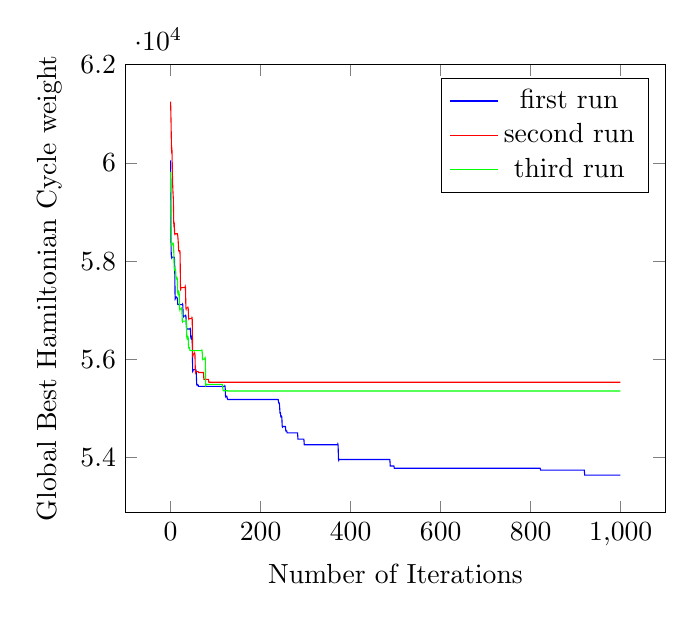
\begin{tikzpicture}
\begin{axis}[
    xlabel={Number of Iterations},
    ylabel={Global Best Hamiltonian Cycle weight},
    legend pos=north east,
    smooth
]
 
\addplot[
    color=blue,smooth
    ]
    coordinates {(0,60053.91441866802)(1,58359.69850730419)(2,58079.775107262445)(3,58079.775107262445)(4,58079.775107262445)(5,58079.775107262445)(6,58079.775107262445)(7,58079.775107262445)(8,58079.775107262445)(9,57949.369238302024)(10,57267.79144641113)(11,57267.79144641113)(12,57267.79144641113)(13,57267.79144641113)(14,57245.77681645975)(15,57245.77681645975)(16,57112.52005640735)(17,57112.52005640735)(18,57112.52005640735)(19,57112.52005640735)(20,57112.52005640735)(21,57112.52005640735)(22,57112.52005640735)(23,57112.52005640735)(24,57112.52005640735)(25,57112.52005640735)(26,57112.52005640735)(27,57112.52005640735)(28,56881.25954175375)(29,56881.25954175375)(30,56881.25954175375)(31,56881.25954175375)(32,56881.25954175375)(33,56881.25954175375)(34,56881.25954175375)(35,56683.90410555623)(36,56616.35791657801)(37,56616.35791657801)(38,56616.35791657801)(39,56616.35791657801)(40,56616.35791657801)(41,56616.35791657801)(42,56616.35791657801)(43,56616.35791657801)(44,56616.35791657801)(45,56430.00108344287)(46,56430.00108344287)(47,56430.00108344287)(48,56430.00108344287)(49,55788.02426694156)(50,55788.02426694156)(51,55788.02426694156)(52,55788.02426694156)(53,55788.02426694156)(54,55788.02426694156)(55,55788.02426694156)(56,55788.02426694156)(57,55721.301601550294)(58,55489.41855077049)(59,55489.41855077049)(60,55478.12231558228)(61,55478.12231558228)(62,55448.469723091795)(63,55448.46972309179)(64,55448.46972309179)(65,55448.46972309179)(66,55448.46972309179)(67,55448.46972309179)(68,55448.46972309179)(69,55448.46972309179)(70,55448.46972309179)(71,55448.46972309179)(72,55448.46972309179)(73,55448.46972309179)(74,55448.46972309179)(75,55448.46972309179)(76,55448.46972309179)(77,55448.46972309179)(78,55448.46972309178)(79,55448.46972309178)(80,55448.46972309178)(81,55448.46972309178)(82,55448.46972309178)(83,55448.46972309178)(84,55448.46972309178)(85,55448.46972309178)(86,55448.46972309178)(87,55448.46972309178)(88,55448.46972309178)(89,55448.46972309178)(90,55448.46972309178)(91,55448.46972309178)(92,55448.46972309178)(93,55448.46972309178)(94,55448.46972309178)(95,55448.46972309178)(96,55448.46972309178)(97,55448.46972309178)(98,55448.46972309178)(99,55448.46972309178)(100,55448.46972309178)(101,55448.46972309178)(102,55448.46972309178)(103,55448.46972309178)(104,55448.46972309178)(105,55448.46972309178)(106,55448.46972309178)(107,55448.46972309178)(108,55448.46972309178)(109,55448.46972309178)(110,55448.46972309178)(111,55448.46972309178)(112,55448.46972309178)(113,55448.46972309178)(114,55448.46972309178)(115,55448.46972309178)(116,55448.46972309178)(117,55448.46972309178)(118,55448.46972309178)(119,55448.46972309178)(120,55448.46972309178)(121,55448.46972309178)(122,55246.75379085121)(123,55246.7537908512)(124,55246.7537908512)(125,55246.7537908512)(126,55196.33169553296)(127,55180.82304552119)(128,55180.82304552119)(129,55180.82304552119)(130,55180.82304552119)(131,55180.82304552119)(132,55180.82304552119)(133,55180.82304552119)(134,55180.82304552119)(135,55180.82304552119)(136,55180.82304552119)(137,55180.82304552119)(138,55180.82304552119)(139,55180.82304552119)(140,55180.82304552119)(141,55180.82304552119)(142,55180.82304552119)(143,55180.82304552119)(144,55180.82304552119)(145,55180.82304552119)(146,55180.82304552119)(147,55180.82304552119)(148,55180.82304552119)(149,55180.82304552119)(150,55180.82304552119)(151,55180.82304552119)(152,55180.82304552119)(153,55180.82304552119)(154,55180.82304552119)(155,55180.82304552119)(156,55180.82304552119)(157,55180.82304552119)(158,55180.82304552119)(159,55180.82304552119)(160,55180.82304552119)(161,55180.82304552119)(162,55180.82304552119)(163,55180.82304552119)(164,55180.82304552119)(165,55180.82304552119)(166,55180.82304552119)(167,55180.82304552119)(168,55180.82304552119)(169,55180.82304552119)(170,55180.82304552119)(171,55180.82304552119)(172,55180.82304552119)(173,55180.82304552119)(174,55180.82304552119)(175,55180.82304552119)(176,55180.82304552119)(177,55180.82304552119)(178,55180.82304552119)(179,55180.82304552119)(180,55180.82304552119)(181,55180.82304552119)(182,55180.82304552119)(183,55180.82304552119)(184,55180.82304552119)(185,55180.82304552119)(186,55180.82304552119)(187,55180.82304552119)(188,55180.82304552119)(189,55180.82304552119)(190,55180.82304552119)(191,55180.82304552119)(192,55180.82304552119)(193,55180.82304552119)(194,55180.82304552119)(195,55180.82304552119)(196,55180.82304552119)(197,55180.82304552119)(198,55180.82304552119)(199,55180.82304552119)(200,55180.82304552119)(201,55180.82304552119)(202,55180.82304552119)(203,55180.82304552119)(204,55180.82304552119)(205,55180.82304552119)(206,55180.82304552119)(207,55180.82304552119)(208,55180.82304552119)(209,55180.82304552118)(210,55180.82304552118)(211,55180.82304552118)(212,55180.82304552118)(213,55180.82304552118)(214,55180.82304552118)(215,55180.82304552118)(216,55180.82304552118)(217,55180.82304552118)(218,55180.82304552118)(219,55180.82304552118)(220,55180.82304552118)(221,55180.82304552118)(222,55180.82304552118)(223,55180.82304552118)(224,55180.82304552118)(225,55180.82304552118)(226,55180.82304552118)(227,55180.82304552118)(228,55180.82304552118)(229,55180.82304552118)(230,55180.82304552118)(231,55180.82304552118)(232,55180.82304552118)(233,55180.82304552118)(234,55180.82304552118)(235,55180.82304552118)(236,55180.82304552118)(237,55180.82304552118)(238,55180.82304552118)(239,55180.82304552118)(240,55115.48472730248)(241,55115.48472730248)(242,55064.21553314375)(243,54903.689396996866)(244,54903.689396996866)(245,54823.240824524146)(246,54823.240824524146)(247,54823.240824524146)(248,54631.41856135874)(249,54631.41856135874)(250,54631.41856135874)(251,54631.41856135874)(252,54631.41856135874)(253,54631.41856135874)(254,54631.41856135874)(255,54631.41856135874)(256,54539.07760999644)(257,54539.07760999644)(258,54539.07760999644)(259,54500.4173601251)(260,54500.4173601251)(261,54500.4173601251)(262,54500.4173601251)(263,54500.4173601251)(264,54500.4173601251)(265,54500.4173601251)(266,54500.4173601251)(267,54500.4173601251)(268,54500.4173601251)(269,54500.4173601251)(270,54500.4173601251)(271,54500.4173601251)(272,54500.4173601251)(273,54500.4173601251)(274,54500.4173601251)(275,54500.4173601251)(276,54500.4173601251)(277,54500.4173601251)(278,54500.4173601251)(279,54500.4173601251)(280,54500.4173601251)(281,54500.4173601251)(282,54500.417360125095)(283,54372.26872285972)(284,54372.26872285972)(285,54372.26872285972)(286,54372.26872285972)(287,54372.26872285972)(288,54372.26872285972)(289,54372.26872285972)(290,54372.26872285972)(291,54372.26872285972)(292,54372.26872285972)(293,54372.26872285972)(294,54372.26872285972)(295,54372.26872285972)(296,54372.26872285972)(297,54258.16316889852)(298,54258.16316889852)(299,54258.16316889852)(300,54258.16316889852)(301,54258.16316889852)(302,54258.16316889852)(303,54258.16316889852)(304,54258.16316889852)(305,54258.16316889852)(306,54258.16316889852)(307,54258.16316889852)(308,54258.16316889852)(309,54258.16316889852)(310,54258.16316889852)(311,54258.16316889852)(312,54258.16316889852)(313,54258.16316889852)(314,54258.16316889852)(315,54258.16316889852)(316,54258.16316889852)(317,54258.16316889852)(318,54258.16316889852)(319,54258.16316889852)(320,54258.16316889852)(321,54258.16316889852)(322,54258.16316889852)(323,54258.16316889852)(324,54258.16316889852)(325,54258.16316889852)(326,54258.16316889852)(327,54258.16316889852)(328,54258.16316889852)(329,54258.16316889852)(330,54258.16316889852)(331,54258.16316889852)(332,54258.16316889852)(333,54258.16316889852)(334,54258.16316889852)(335,54258.16316889852)(336,54258.16316889852)(337,54258.16316889852)(338,54258.16316889852)(339,54258.16316889852)(340,54258.16316889852)(341,54258.16316889852)(342,54258.16316889852)(343,54258.16316889852)(344,54258.16316889852)(345,54258.16316889852)(346,54258.16316889852)(347,54258.16316889852)(348,54258.16316889852)(349,54258.16316889852)(350,54258.16316889852)(351,54258.16316889852)(352,54258.16316889852)(353,54258.16316889852)(354,54258.16316889852)(355,54258.16316889852)(356,54258.16316889852)(357,54258.16316889852)(358,54258.16316889852)(359,54258.16316889852)(360,54258.16316889852)(361,54258.16316889852)(362,54258.16316889852)(363,54258.16316889852)(364,54258.16316889852)(365,54258.16316889852)(366,54258.16316889852)(367,54258.16316889852)(368,54258.16316889852)(369,54258.16316889852)(370,54258.16316889852)(371,54258.16316889852)(372,54258.16316889852)(373,53958.50916256144)(374,53958.50916256144)(375,53958.50916256144)(376,53958.50916256144)(377,53958.50916256144)(378,53958.50916256144)(379,53958.50916256144)(380,53958.50916256144)(381,53958.50916256143)(382,53958.50916256143)(383,53958.50916256143)(384,53958.50916256143)(385,53958.50916256143)(386,53958.50916256143)(387,53958.50916256143)(388,53958.50916256143)(389,53958.50916256143)(390,53958.50916256143)(391,53958.50916256143)(392,53958.50916256143)(393,53958.50916256143)(394,53958.50916256143)(395,53958.50916256143)(396,53958.50916256143)(397,53958.50916256143)(398,53958.50916256143)(399,53958.50916256143)(400,53958.50916256143)(401,53958.50916256143)(402,53958.50916256143)(403,53958.50916256143)(404,53958.50916256143)(405,53958.50916256143)(406,53958.50916256143)(407,53958.50916256143)(408,53958.50916256143)(409,53958.50916256143)(410,53958.50916256143)(411,53958.50916256143)(412,53958.50916256143)(413,53958.50916256143)(414,53958.50916256143)(415,53958.50916256143)(416,53958.50916256143)(417,53958.50916256143)(418,53958.50916256143)(419,53958.50916256143)(420,53958.50916256143)(421,53958.50916256143)(422,53958.50916256143)(423,53958.50916256143)(424,53958.50916256143)(425,53958.50916256143)(426,53958.50916256143)(427,53958.50916256143)(428,53958.50916256143)(429,53958.50916256143)(430,53958.50916256143)(431,53958.50916256143)(432,53958.50916256143)(433,53958.50916256143)(434,53958.50916256143)(435,53958.50916256143)(436,53958.50916256143)(437,53958.50916256143)(438,53958.50916256143)(439,53958.50916256143)(440,53958.50916256143)(441,53958.50916256143)(442,53958.50916256143)(443,53958.50916256143)(444,53958.50916256143)(445,53958.50916256143)(446,53958.50916256143)(447,53958.50916256143)(448,53958.50916256143)(449,53958.50916256143)(450,53958.50916256143)(451,53958.50916256143)(452,53958.50916256143)(453,53958.50916256143)(454,53958.50916256143)(455,53958.50916256143)(456,53958.50916256143)(457,53958.50916256143)(458,53958.50916256143)(459,53958.50916256143)(460,53958.50916256143)(461,53958.50916256143)(462,53958.50916256143)(463,53958.50916256143)(464,53958.50916256143)(465,53958.50916256143)(466,53958.50916256143)(467,53958.50916256143)(468,53958.50916256143)(469,53958.50916256143)(470,53958.50916256143)(471,53958.50916256143)(472,53958.50916256143)(473,53958.50916256143)(474,53958.50916256143)(475,53958.50916256143)(476,53958.50916256143)(477,53958.50916256143)(478,53958.50916256143)(479,53958.50916256143)(480,53958.50916256143)(481,53958.50916256143)(482,53958.50916256143)(483,53958.50916256143)(484,53958.50916256143)(485,53958.50916256143)(486,53958.50916256143)(487,53958.50916256143)(488,53826.16868064484)(489,53826.16868064484)(490,53826.16868064484)(491,53826.16868064484)(492,53826.16868064484)(493,53826.16868064484)(494,53826.16868064484)(495,53826.16868064484)(496,53826.16868064484)(497,53779.701864029885)(498,53779.701864029885)(499,53779.701864029885)(500,53779.701864029885)(501,53779.701864029885)(502,53779.701864029885)(503,53779.701864029885)(504,53779.701864029885)(505,53779.701864029885)(506,53779.701864029885)(507,53779.701864029885)(508,53779.701864029885)(509,53779.701864029885)(510,53779.701864029885)(511,53779.701864029885)(512,53779.701864029885)(513,53779.701864029885)(514,53779.701864029885)(515,53779.701864029885)(516,53779.701864029885)(517,53779.701864029885)(518,53779.701864029885)(519,53779.701864029885)(520,53779.701864029885)(521,53779.701864029885)(522,53779.701864029885)(523,53779.701864029885)(524,53779.701864029885)(525,53779.701864029885)(526,53779.701864029885)(527,53779.701864029885)(528,53779.701864029885)(529,53779.701864029885)(530,53779.701864029885)(531,53779.701864029885)(532,53779.701864029885)(533,53779.701864029885)(534,53779.701864029885)(535,53779.701864029885)(536,53779.701864029885)(537,53779.701864029885)(538,53779.701864029885)(539,53779.701864029885)(540,53779.701864029885)(541,53779.701864029885)(542,53779.701864029885)(543,53779.701864029885)(544,53779.701864029885)(545,53779.701864029885)(546,53779.701864029885)(547,53779.701864029885)(548,53779.701864029885)(549,53779.701864029885)(550,53779.701864029885)(551,53779.701864029885)(552,53779.701864029885)(553,53779.701864029885)(554,53779.70186402988)(555,53779.70186402988)(556,53779.70186402988)(557,53779.70186402988)(558,53779.70186402988)(559,53779.70186402988)(560,53779.70186402988)(561,53779.70186402988)(562,53779.70186402988)(563,53779.70186402988)(564,53779.70186402988)(565,53779.70186402988)(566,53779.70186402988)(567,53779.70186402988)(568,53779.70186402988)(569,53779.70186402988)(570,53779.70186402988)(571,53779.70186402988)(572,53779.70186402988)(573,53779.70186402988)(574,53779.70186402988)(575,53779.70186402988)(576,53779.70186402988)(577,53779.70186402988)(578,53779.70186402988)(579,53779.70186402988)(580,53779.70186402988)(581,53779.70186402988)(582,53779.70186402988)(583,53779.70186402988)(584,53779.70186402988)(585,53779.70186402988)(586,53779.70186402988)(587,53779.70186402988)(588,53779.70186402988)(589,53779.70186402988)(590,53779.70186402988)(591,53779.70186402988)(592,53779.70186402988)(593,53779.70186402988)(594,53779.70186402988)(595,53779.70186402988)(596,53779.70186402988)(597,53779.70186402988)(598,53779.70186402988)(599,53779.70186402987)(600,53779.70186402987)(601,53779.70186402987)(602,53779.70186402987)(603,53779.70186402987)(604,53779.70186402987)(605,53779.70186402987)(606,53779.70186402987)(607,53779.70186402987)(608,53779.70186402987)(609,53779.70186402987)(610,53779.70186402987)(611,53779.70186402987)(612,53779.70186402987)(613,53779.70186402987)(614,53779.70186402987)(615,53779.70186402987)(616,53779.70186402987)(617,53779.70186402987)(618,53779.70186402987)(619,53779.70186402987)(620,53779.70186402987)(621,53779.70186402987)(622,53779.70186402987)(623,53779.70186402987)(624,53779.70186402987)(625,53779.70186402987)(626,53779.70186402987)(627,53779.70186402987)(628,53779.70186402987)(629,53779.70186402987)(630,53779.70186402987)(631,53779.70186402987)(632,53779.70186402987)(633,53779.70186402987)(634,53779.70186402987)(635,53779.70186402987)(636,53779.70186402987)(637,53779.70186402987)(638,53779.70186402987)(639,53779.70186402987)(640,53779.70186402987)(641,53779.70186402987)(642,53779.70186402987)(643,53779.70186402987)(644,53779.70186402987)(645,53779.70186402987)(646,53779.70186402987)(647,53779.70186402987)(648,53779.70186402987)(649,53779.70186402987)(650,53779.70186402987)(651,53779.70186402987)(652,53779.70186402987)(653,53779.70186402987)(654,53779.70186402987)(655,53779.70186402987)(656,53779.70186402987)(657,53779.70186402987)(658,53779.70186402987)(659,53779.70186402987)(660,53779.70186402987)(661,53779.70186402987)(662,53779.70186402987)(663,53779.70186402987)(664,53779.70186402987)(665,53779.70186402987)(666,53779.70186402987)(667,53779.70186402987)(668,53779.70186402987)(669,53779.70186402987)(670,53779.70186402987)(671,53779.70186402987)(672,53779.70186402987)(673,53779.70186402987)(674,53779.70186402987)(675,53779.70186402987)(676,53779.70186402987)(677,53779.70186402987)(678,53779.70186402987)(679,53779.70186402987)(680,53779.70186402987)(681,53779.70186402987)(682,53779.70186402987)(683,53779.70186402987)(684,53779.70186402987)(685,53779.70186402987)(686,53779.70186402987)(687,53779.70186402987)(688,53779.70186402987)(689,53779.70186402987)(690,53779.70186402987)(691,53779.70186402987)(692,53779.70186402987)(693,53779.70186402987)(694,53779.70186402987)(695,53779.70186402987)(696,53779.70186402987)(697,53779.70186402987)(698,53779.70186402987)(699,53779.70186402987)(700,53779.70186402987)(701,53779.70186402987)(702,53779.70186402987)(703,53779.70186402987)(704,53779.70186402987)(705,53779.70186402987)(706,53779.70186402987)(707,53779.70186402987)(708,53779.70186402987)(709,53779.70186402987)(710,53779.70186402987)(711,53779.70186402987)(712,53779.70186402987)(713,53779.70186402987)(714,53779.70186402987)(715,53779.70186402987)(716,53779.70186402987)(717,53779.70186402987)(718,53779.70186402987)(719,53779.70186402987)(720,53779.70186402987)(721,53779.70186402987)(722,53779.70186402987)(723,53779.70186402987)(724,53779.70186402987)(725,53779.70186402987)(726,53779.70186402987)(727,53779.70186402987)(728,53779.70186402987)(729,53779.70186402987)(730,53779.70186402987)(731,53779.70186402987)(732,53779.70186402987)(733,53779.70186402987)(734,53779.70186402987)(735,53779.70186402987)(736,53779.70186402987)(737,53779.70186402987)(738,53779.70186402987)(739,53779.70186402987)(740,53779.70186402987)(741,53779.70186402987)(742,53779.70186402987)(743,53779.70186402987)(744,53779.70186402987)(745,53779.70186402987)(746,53779.70186402987)(747,53779.70186402987)(748,53779.70186402987)(749,53779.70186402987)(750,53779.70186402987)(751,53779.70186402987)(752,53779.70186402987)(753,53779.70186402987)(754,53779.70186402987)(755,53779.70186402987)(756,53779.70186402987)(757,53779.70186402987)(758,53779.70186402987)(759,53779.70186402987)(760,53779.70186402987)(761,53779.70186402987)(762,53779.70186402987)(763,53779.70186402987)(764,53779.70186402987)(765,53779.70186402987)(766,53779.70186402987)(767,53779.70186402987)(768,53779.70186402987)(769,53779.70186402987)(770,53779.70186402987)(771,53779.70186402987)(772,53779.70186402987)(773,53779.70186402987)(774,53779.70186402987)(775,53779.70186402987)(776,53779.70186402987)(777,53779.70186402987)(778,53779.70186402987)(779,53779.70186402987)(780,53779.70186402987)(781,53779.70186402987)(782,53779.70186402987)(783,53779.70186402987)(784,53779.70186402987)(785,53779.70186402987)(786,53779.70186402987)(787,53779.70186402987)(788,53779.70186402987)(789,53779.70186402987)(790,53779.70186402987)(791,53779.70186402987)(792,53779.70186402987)(793,53779.70186402987)(794,53779.70186402987)(795,53779.70186402987)(796,53779.70186402987)(797,53779.70186402987)(798,53779.70186402987)(799,53779.70186402987)(800,53779.70186402987)(801,53779.70186402987)(802,53779.70186402987)(803,53779.70186402987)(804,53779.70186402987)(805,53779.70186402987)(806,53779.70186402987)(807,53779.70186402987)(808,53779.70186402987)(809,53779.70186402987)(810,53779.70186402987)(811,53779.70186402987)(812,53779.70186402987)(813,53779.70186402987)(814,53779.70186402987)(815,53779.70186402987)(816,53779.70186402987)(817,53779.70186402987)(818,53779.70186402987)(819,53779.70186402987)(820,53779.70186402987)(821,53779.70186402987)(822,53743.137497600095)(823,53743.137497600095)(824,53743.137497600095)(825,53743.137497600095)(826,53743.137497600095)(827,53743.137497600095)(828,53743.137497600095)(829,53743.137497600095)(830,53743.137497600095)(831,53743.137497600095)(832,53743.137497600095)(833,53743.137497600095)(834,53743.137497600095)(835,53743.137497600095)(836,53743.137497600095)(837,53743.137497600095)(838,53743.137497600095)(839,53743.137497600095)(840,53743.137497600095)(841,53743.137497600095)(842,53743.137497600095)(843,53743.137497600095)(844,53743.137497600095)(845,53743.137497600095)(846,53743.137497600095)(847,53743.137497600095)(848,53743.137497600095)(849,53743.137497600095)(850,53743.137497600095)(851,53743.137497600095)(852,53743.137497600095)(853,53743.137497600095)(854,53743.137497600095)(855,53743.137497600095)(856,53743.137497600095)(857,53743.137497600095)(858,53743.137497600095)(859,53743.137497600095)(860,53743.137497600095)(861,53743.137497600095)(862,53743.137497600095)(863,53743.137497600095)(864,53743.137497600095)(865,53743.137497600095)(866,53743.137497600095)(867,53743.137497600095)(868,53743.137497600095)(869,53743.137497600095)(870,53743.137497600095)(871,53743.137497600095)(872,53743.137497600095)(873,53743.137497600095)(874,53743.137497600095)(875,53743.137497600095)(876,53743.137497600095)(877,53743.137497600095)(878,53743.137497600095)(879,53743.137497600095)(880,53743.137497600095)(881,53743.137497600095)(882,53743.137497600095)(883,53743.137497600095)(884,53743.137497600095)(885,53743.137497600095)(886,53743.137497600095)(887,53743.137497600095)(888,53743.137497600095)(889,53743.137497600095)(890,53743.137497600095)(891,53743.137497600095)(892,53743.137497600095)(893,53743.137497600095)(894,53743.137497600095)(895,53743.137497600095)(896,53743.137497600095)(897,53743.137497600095)(898,53743.137497600095)(899,53743.137497600095)(900,53743.137497600095)(901,53743.137497600095)(902,53743.137497600095)(903,53743.137497600095)(904,53743.137497600095)(905,53743.137497600095)(906,53743.137497600095)(907,53743.137497600095)(908,53743.137497600095)(909,53743.137497600095)(910,53743.137497600095)(911,53743.137497600095)(912,53743.137497600095)(913,53743.137497600095)(914,53743.137497600095)(915,53743.137497600095)(916,53743.137497600095)(917,53743.137497600095)(918,53743.137497600095)(919,53743.137497600095)(920,53639.41397407093)(921,53639.41397407093)(922,53639.41397407093)(923,53639.41397407093)(924,53639.41397407093)(925,53639.41397407093)(926,53639.41397407093)(927,53639.41397407093)(928,53639.41397407093)(929,53639.41397407093)(930,53639.41397407093)(931,53639.41397407093)(932,53639.41397407093)(933,53639.41397407093)(934,53639.41397407093)(935,53639.41397407093)(936,53639.41397407093)(937,53639.41397407093)(938,53639.41397407093)(939,53639.41397407093)(940,53639.41397407093)(941,53639.41397407093)(942,53639.41397407093)(943,53639.41397407093)(944,53639.41397407093)(945,53639.41397407093)(946,53639.41397407093)(947,53639.41397407093)(948,53639.41397407093)(949,53639.41397407093)(950,53639.41397407093)(951,53639.41397407093)(952,53639.41397407093)(953,53639.41397407093)(954,53639.41397407093)(955,53639.41397407093)(956,53639.41397407093)(957,53639.41397407093)(958,53639.41397407093)(959,53639.41397407093)(960,53639.41397407093)(961,53639.41397407093)(962,53639.41397407093)(963,53639.41397407093)(964,53639.41397407093)(965,53639.41397407093)(966,53639.41397407093)(967,53639.41397407093)(968,53639.41397407093)(969,53639.41397407093)(970,53639.41397407093)(971,53639.41397407093)(972,53639.41397407093)(973,53639.41397407093)(974,53639.41397407093)(975,53639.41397407093)(976,53639.41397407093)(977,53639.41397407093)(978,53639.41397407093)(979,53639.41397407093)(980,53639.41397407093)(981,53639.41397407093)(982,53639.41397407093)(983,53639.41397407093)(984,53639.41397407093)(985,53639.41397407093)(986,53639.41397407093)(987,53639.41397407093)(988,53639.41397407093)(989,53639.41397407093)(990,53639.41397407093)(991,53639.41397407093)(992,53639.41397407093)(993,53639.41397407093)(994,53639.41397407093)(995,53639.41397407093)(996,53639.41397407093)(997,53639.41397407093)(998,53639.41397407093)(999,53639.41397407093)
    };
   \addlegendentry{first run}
\addplot[
    color=red,smooth
    ]
    coordinates {
	(0,61249.97723448629)(1,60814.377686011394)(2,60281.671561080955)(3,60256.02919927783)(4,59763.343382177765)(5,59452.22220637821)(6,59276.771798847396)(7,58774.87039775655)(8,58774.87039775655)(9,58557.64522794433)(10,58557.64522794433)(11,58557.64522794433)(12,58557.64522794433)(13,58557.64522794433)(14,58557.64522794433)(15,58557.64522794433)(16,58504.33694605673)(17,58379.910998468964)(18,58214.30625613625)(19,58214.30625613625)(20,58214.30625613625)(21,58135.95061092619)(22,57460.195965748746)(23,57460.195965748746)(24,57460.195965748746)(25,57460.195965748746)(26,57460.195965748746)(27,57460.195965748746)(28,57460.195965748746)(29,57460.195965748746)(30,57460.195965748746)(31,57460.195965748746)(32,57460.195965748746)(33,57460.195965748746)(34,57046.587901164334)(35,57046.587901164334)(36,57046.587901164334)(37,57046.587901164334)(38,57046.587901164334)(39,57046.587901164334)(40,56829.13119955657)(41,56829.13119955657)(42,56829.13119955657)(43,56829.13119955657)(44,56829.13119955657)(45,56829.13119955657)(46,56829.13119955657)(47,56829.13119955657)(48,56809.33849738488)(49,56106.53949524769)(50,56106.53949524769)(51,56106.53949524769)(52,56106.53949524769)(53,56106.53949524769)(54,56106.53949524769)(55,55749.01162312865)(56,55749.01162312865)(57,55749.01162312865)(58,55749.01162312865)(59,55749.01162312865)(60,55749.01162312865)(61,55749.01162312865)(62,55729.60204933076)(63,55729.60204933076)(64,55729.60204933076)(65,55729.60204933076)(66,55729.60204933076)(67,55729.60204933076)(68,55729.60204933076)(69,55729.60204933076)(70,55729.60204933076)(71,55729.60204933075)(72,55729.60204933075)(73,55729.60204933075)(74,55590.157176877154)(75,55590.157176877154)(76,55590.157176877154)(77,55590.157176877154)(78,55590.15717687714)(79,55590.15717687714)(80,55590.15717687714)(81,55590.15717687714)(82,55590.15717687714)(83,55590.15717687714)(84,55590.15717687714)(85,55531.578533114465)(86,55531.57853311445)(87,55531.57853311445)(88,55531.57853311445)(89,55531.57853311445)(90,55531.57853311445)(91,55531.57853311445)(92,55531.57853311445)(93,55531.57853311445)(94,55531.57853311445)(95,55531.57853311445)(96,55531.57853311445)(97,55531.57853311445)(98,55531.57853311445)(99,55531.57853311445)(100,55531.57853311445)(101,55531.57853311445)(102,55531.57853311445)(103,55531.57853311445)(104,55531.57853311445)(105,55531.57853311445)(106,55531.57853311445)(107,55531.57853311445)(108,55531.57853311444)(109,55531.57853311444)(110,55531.57853311444)(111,55531.57853311444)(112,55531.57853311444)(113,55531.57853311444)(114,55531.57853311444)(115,55531.57853311444)(116,55531.57853311444)(117,55531.57853311444)(118,55531.57853311444)(119,55531.57853311444)(120,55531.57853311444)(121,55531.57853311444)(122,55531.57853311444)(123,55531.57853311444)(124,55531.57853311444)(125,55531.57853311444)(126,55531.57853311444)(127,55531.57853311444)(128,55531.57853311444)(129,55531.57853311444)(130,55531.57853311444)(131,55531.57853311444)(132,55531.57853311444)(133,55531.57853311444)(134,55531.57853311444)(135,55531.57853311444)(136,55531.57853311444)(137,55531.57853311444)(138,55531.57853311444)(139,55531.57853311444)(140,55531.57853311444)(141,55531.57853311444)(142,55531.57853311444)(143,55531.57853311444)(144,55531.57853311444)(145,55531.57853311444)(146,55531.57853311444)(147,55531.57853311444)(148,55531.57853311444)(149,55531.57853311444)(150,55531.57853311444)(151,55531.57853311444)(152,55531.57853311444)(153,55531.57853311444)(154,55531.57853311444)(155,55531.57853311444)(156,55531.57853311444)(157,55531.57853311444)(158,55531.57853311444)(159,55531.57853311444)(160,55531.57853311444)(161,55531.57853311444)(162,55531.57853311444)(163,55531.57853311444)(164,55531.57853311444)(165,55531.57853311444)(166,55531.57853311444)(167,55531.57853311444)(168,55531.57853311444)(169,55531.57853311444)(170,55531.57853311444)(171,55531.57853311444)(172,55531.57853311444)(173,55531.57853311444)(174,55531.57853311444)(175,55531.57853311444)(176,55531.57853311444)(177,55531.57853311444)(178,55531.57853311444)(179,55531.57853311444)(180,55531.57853311444)(181,55531.57853311444)(182,55531.57853311444)(183,55531.57853311444)(184,55531.57853311444)(185,55531.57853311444)(186,55531.57853311444)(187,55531.57853311444)(188,55531.57853311444)(189,55531.57853311444)(190,55531.57853311444)(191,55531.57853311444)(192,55531.57853311444)(193,55531.57853311444)(194,55531.57853311444)(195,55531.57853311444)(196,55531.57853311444)(197,55531.57853311444)(198,55531.57853311444)(199,55531.57853311444)(200,55531.57853311444)(201,55531.57853311444)(202,55531.57853311444)(203,55531.57853311444)(204,55531.57853311444)(205,55531.57853311444)(206,55531.57853311444)(207,55531.57853311444)(208,55531.57853311444)(209,55531.57853311444)(210,55531.57853311444)(211,55531.57853311444)(212,55531.57853311444)(213,55531.57853311444)(214,55531.57853311444)(215,55531.57853311444)(216,55531.57853311444)(217,55531.57853311444)(218,55531.57853311444)(219,55531.57853311444)(220,55531.57853311444)(221,55531.57853311444)(222,55531.57853311444)(223,55531.57853311444)(224,55531.57853311444)(225,55531.57853311444)(226,55531.57853311444)(227,55531.57853311444)(228,55531.57853311444)(229,55531.57853311444)(230,55531.57853311444)(231,55531.57853311444)(232,55531.57853311444)(233,55531.57853311444)(234,55531.57853311444)(235,55531.57853311444)(236,55531.57853311444)(237,55531.57853311444)(238,55531.57853311444)(239,55531.57853311444)(240,55531.57853311444)(241,55531.57853311444)(242,55531.57853311444)(243,55531.57853311444)(244,55531.57853311444)(245,55531.57853311444)(246,55531.57853311444)(247,55531.57853311444)(248,55531.57853311444)(249,55531.57853311444)(250,55531.57853311444)(251,55531.57853311444)(252,55531.57853311444)(253,55531.57853311444)(254,55531.57853311444)(255,55531.57853311444)(256,55531.57853311444)(257,55531.57853311444)(258,55531.57853311444)(259,55531.57853311444)(260,55531.57853311444)(261,55531.57853311444)(262,55531.57853311444)(263,55531.57853311444)(264,55531.57853311444)(265,55531.57853311444)(266,55531.57853311444)(267,55531.57853311444)(268,55531.57853311444)(269,55531.57853311444)(270,55531.57853311444)(271,55531.57853311444)(272,55531.57853311444)(273,55531.57853311444)(274,55531.57853311444)(275,55531.57853311444)(276,55531.57853311444)(277,55531.57853311444)(278,55531.57853311444)(279,55531.57853311444)(280,55531.57853311444)(281,55531.57853311444)(282,55531.57853311444)(283,55531.57853311444)(284,55531.57853311444)(285,55531.57853311444)(286,55531.57853311444)(287,55531.57853311444)(288,55531.57853311444)(289,55531.57853311444)(290,55531.57853311444)(291,55531.57853311444)(292,55531.57853311444)(293,55531.57853311444)(294,55531.57853311444)(295,55531.57853311444)(296,55531.57853311444)(297,55531.57853311444)(298,55531.57853311444)(299,55531.57853311444)(300,55531.57853311444)(301,55531.57853311444)(302,55531.57853311444)(303,55531.57853311444)(304,55531.57853311444)(305,55531.57853311444)(306,55531.57853311444)(307,55531.57853311444)(308,55531.57853311444)(309,55531.57853311444)(310,55531.57853311444)(311,55531.57853311444)(312,55531.57853311444)(313,55531.57853311444)(314,55531.57853311444)(315,55531.57853311444)(316,55531.57853311444)(317,55531.57853311444)(318,55531.57853311444)(319,55531.57853311444)(320,55531.57853311444)(321,55531.57853311444)(322,55531.57853311444)(323,55531.57853311444)(324,55531.57853311444)(325,55531.57853311444)(326,55531.57853311444)(327,55531.57853311444)(328,55531.57853311444)(329,55531.57853311444)(330,55531.57853311444)(331,55531.57853311444)(332,55531.57853311444)(333,55531.57853311444)(334,55531.57853311444)(335,55531.57853311444)(336,55531.57853311444)(337,55531.57853311444)(338,55531.57853311444)(339,55531.57853311444)(340,55531.57853311444)(341,55531.57853311444)(342,55531.57853311444)(343,55531.57853311444)(344,55531.57853311444)(345,55531.57853311444)(346,55531.57853311444)(347,55531.57853311444)(348,55531.57853311444)(349,55531.57853311444)(350,55531.57853311444)(351,55531.57853311444)(352,55531.57853311444)(353,55531.57853311444)(354,55531.57853311444)(355,55531.57853311444)(356,55531.57853311444)(357,55531.57853311444)(358,55531.57853311444)(359,55531.57853311444)(360,55531.57853311444)(361,55531.57853311444)(362,55531.57853311444)(363,55531.57853311444)(364,55531.57853311444)(365,55531.57853311444)(366,55531.57853311444)(367,55531.57853311444)(368,55531.57853311444)(369,55531.57853311444)(370,55531.57853311444)(371,55531.57853311444)(372,55531.57853311444)(373,55531.57853311444)(374,55531.57853311444)(375,55531.57853311444)(376,55531.57853311444)(377,55531.57853311444)(378,55531.57853311444)(379,55531.57853311444)(380,55531.57853311444)(381,55531.57853311444)(382,55531.57853311444)(383,55531.57853311444)(384,55531.57853311444)(385,55531.57853311444)(386,55531.57853311444)(387,55531.57853311444)(388,55531.57853311444)(389,55531.57853311444)(390,55531.57853311444)(391,55531.57853311444)(392,55531.57853311444)(393,55531.57853311444)(394,55531.57853311444)(395,55531.57853311444)(396,55531.57853311444)(397,55531.57853311444)(398,55531.57853311444)(399,55531.57853311444)(400,55531.57853311444)(401,55531.57853311444)(402,55531.57853311444)(403,55531.57853311444)(404,55531.57853311444)(405,55531.57853311444)(406,55531.57853311444)(407,55531.57853311444)(408,55531.57853311444)(409,55531.57853311444)(410,55531.57853311444)(411,55531.57853311444)(412,55531.57853311444)(413,55531.57853311444)(414,55531.57853311444)(415,55531.57853311444)(416,55531.57853311444)(417,55531.57853311444)(418,55531.57853311444)(419,55531.57853311444)(420,55531.57853311444)(421,55531.57853311444)(422,55531.57853311444)(423,55531.57853311444)(424,55531.57853311444)(425,55531.57853311444)(426,55531.57853311444)(427,55531.57853311444)(428,55531.57853311444)(429,55531.57853311444)(430,55531.57853311444)(431,55531.57853311444)(432,55531.57853311444)(433,55531.57853311444)(434,55531.57853311444)(435,55531.57853311444)(436,55531.57853311444)(437,55531.57853311444)(438,55531.57853311444)(439,55531.57853311444)(440,55531.57853311444)(441,55531.57853311444)(442,55531.57853311444)(443,55531.57853311444)(444,55531.57853311444)(445,55531.57853311444)(446,55531.57853311444)(447,55531.57853311444)(448,55531.57853311444)(449,55531.57853311444)(450,55531.57853311444)(451,55531.57853311444)(452,55531.57853311444)(453,55531.57853311444)(454,55531.57853311444)(455,55531.57853311444)(456,55531.57853311444)(457,55531.57853311444)(458,55531.57853311444)(459,55531.57853311444)(460,55531.57853311444)(461,55531.57853311444)(462,55531.57853311444)(463,55531.57853311444)(464,55531.57853311444)(465,55531.57853311444)(466,55531.57853311444)(467,55531.57853311444)(468,55531.57853311444)(469,55531.57853311444)(470,55531.57853311444)(471,55531.57853311444)(472,55531.57853311444)(473,55531.57853311444)(474,55531.57853311444)(475,55531.57853311444)(476,55531.57853311444)(477,55531.57853311444)(478,55531.57853311444)(479,55531.57853311444)(480,55531.57853311444)(481,55531.57853311444)(482,55531.57853311444)(483,55531.57853311444)(484,55531.57853311444)(485,55531.57853311444)(486,55531.57853311444)(487,55531.57853311444)(488,55531.57853311444)(489,55531.57853311444)(490,55531.57853311444)(491,55531.57853311444)(492,55531.57853311444)(493,55531.57853311444)(494,55531.57853311444)(495,55531.57853311444)(496,55531.57853311444)(497,55531.57853311444)(498,55531.57853311444)(499,55531.57853311444)(500,55531.57853311444)(501,55531.57853311444)(502,55531.57853311444)(503,55531.57853311444)(504,55531.57853311444)(505,55531.57853311444)(506,55531.57853311444)(507,55531.57853311444)(508,55531.57853311444)(509,55531.57853311444)(510,55531.57853311444)(511,55531.57853311444)(512,55531.57853311444)(513,55531.57853311444)(514,55531.57853311444)(515,55531.57853311444)(516,55531.57853311444)(517,55531.57853311444)(518,55531.57853311444)(519,55531.57853311444)(520,55531.57853311444)(521,55531.57853311444)(522,55531.57853311444)(523,55531.57853311444)(524,55531.57853311444)(525,55531.57853311444)(526,55531.57853311444)(527,55531.57853311444)(528,55531.57853311444)(529,55531.57853311444)(530,55531.57853311444)(531,55531.57853311444)(532,55531.57853311444)(533,55531.57853311444)(534,55531.57853311444)(535,55531.57853311444)(536,55531.57853311444)(537,55531.57853311444)(538,55531.57853311444)(539,55531.57853311444)(540,55531.57853311444)(541,55531.57853311444)(542,55531.57853311444)(543,55531.57853311444)(544,55531.57853311444)(545,55531.57853311444)(546,55531.57853311444)(547,55531.57853311444)(548,55531.57853311444)(549,55531.57853311444)(550,55531.57853311444)(551,55531.57853311444)(552,55531.57853311444)(553,55531.57853311444)(554,55531.57853311444)(555,55531.57853311444)(556,55531.57853311444)(557,55531.57853311444)(558,55531.57853311444)(559,55531.57853311444)(560,55531.57853311444)(561,55531.57853311444)(562,55531.57853311444)(563,55531.57853311444)(564,55531.57853311444)(565,55531.57853311444)(566,55531.57853311444)(567,55531.57853311444)(568,55531.57853311444)(569,55531.57853311444)(570,55531.57853311444)(571,55531.57853311444)(572,55531.57853311444)(573,55531.57853311444)(574,55531.57853311444)(575,55531.57853311444)(576,55531.57853311444)(577,55531.57853311444)(578,55531.57853311444)(579,55531.57853311444)(580,55531.57853311444)(581,55531.57853311444)(582,55531.57853311444)(583,55531.57853311444)(584,55531.57853311444)(585,55531.57853311444)(586,55531.57853311444)(587,55531.57853311444)(588,55531.57853311444)(589,55531.57853311444)(590,55531.57853311444)(591,55531.57853311444)(592,55531.57853311444)(593,55531.57853311444)(594,55531.57853311444)(595,55531.57853311444)(596,55531.57853311444)(597,55531.57853311444)(598,55531.57853311444)(599,55531.57853311444)(600,55531.57853311444)(601,55531.57853311444)(602,55531.57853311444)(603,55531.57853311444)(604,55531.57853311444)(605,55531.57853311444)(606,55531.57853311444)(607,55531.57853311444)(608,55531.57853311444)(609,55531.57853311444)(610,55531.57853311444)(611,55531.57853311444)(612,55531.57853311444)(613,55531.57853311444)(614,55531.57853311444)(615,55531.57853311444)(616,55531.57853311444)(617,55531.57853311444)(618,55531.57853311444)(619,55531.57853311444)(620,55531.57853311444)(621,55531.57853311444)(622,55531.57853311444)(623,55531.57853311444)(624,55531.57853311444)(625,55531.57853311444)(626,55531.57853311444)(627,55531.57853311444)(628,55531.57853311444)(629,55531.57853311444)(630,55531.57853311444)(631,55531.57853311444)(632,55531.57853311444)(633,55531.57853311444)(634,55531.57853311444)(635,55531.57853311444)(636,55531.57853311444)(637,55531.57853311444)(638,55531.57853311444)(639,55531.57853311444)(640,55531.57853311444)(641,55531.57853311444)(642,55531.57853311444)(643,55531.57853311444)(644,55531.57853311444)(645,55531.57853311444)(646,55531.57853311444)(647,55531.57853311444)(648,55531.57853311444)(649,55531.57853311444)(650,55531.57853311444)(651,55531.57853311444)(652,55531.57853311444)(653,55531.57853311444)(654,55531.57853311444)(655,55531.57853311444)(656,55531.57853311444)(657,55531.57853311444)(658,55531.57853311444)(659,55531.57853311444)(660,55531.57853311444)(661,55531.57853311444)(662,55531.57853311444)(663,55531.57853311444)(664,55531.57853311444)(665,55531.57853311444)(666,55531.57853311444)(667,55531.57853311444)(668,55531.57853311444)(669,55531.57853311444)(670,55531.57853311444)(671,55531.57853311444)(672,55531.57853311444)(673,55531.57853311444)(674,55531.57853311444)(675,55531.57853311444)(676,55531.57853311444)(677,55531.57853311444)(678,55531.57853311444)(679,55531.57853311444)(680,55531.57853311444)(681,55531.57853311444)(682,55531.57853311444)(683,55531.57853311444)(684,55531.57853311444)(685,55531.57853311444)(686,55531.57853311444)(687,55531.57853311444)(688,55531.57853311444)(689,55531.57853311444)(690,55531.57853311444)(691,55531.57853311444)(692,55531.57853311444)(693,55531.57853311444)(694,55531.57853311444)(695,55531.57853311444)(696,55531.57853311444)(697,55531.57853311444)(698,55531.57853311444)(699,55531.57853311444)(700,55531.57853311444)(701,55531.57853311444)(702,55531.57853311444)(703,55531.57853311444)(704,55531.57853311444)(705,55531.57853311444)(706,55531.57853311444)(707,55531.57853311444)(708,55531.57853311444)(709,55531.57853311444)(710,55531.57853311444)(711,55531.57853311444)(712,55531.57853311444)(713,55531.57853311444)(714,55531.57853311444)(715,55531.57853311444)(716,55531.57853311444)(717,55531.57853311444)(718,55531.57853311444)(719,55531.57853311444)(720,55531.57853311444)(721,55531.57853311444)(722,55531.57853311444)(723,55531.57853311444)(724,55531.57853311444)(725,55531.57853311444)(726,55531.57853311444)(727,55531.57853311444)(728,55531.57853311444)(729,55531.57853311444)(730,55531.57853311444)(731,55531.57853311444)(732,55531.57853311444)(733,55531.57853311444)(734,55531.57853311444)(735,55531.57853311444)(736,55531.57853311444)(737,55531.57853311444)(738,55531.57853311444)(739,55531.57853311444)(740,55531.57853311444)(741,55531.57853311444)(742,55531.57853311444)(743,55531.57853311444)(744,55531.57853311444)(745,55531.57853311444)(746,55531.57853311444)(747,55531.57853311444)(748,55531.57853311444)(749,55531.57853311444)(750,55531.57853311444)(751,55531.57853311444)(752,55531.57853311444)(753,55531.57853311444)(754,55531.57853311444)(755,55531.57853311444)(756,55531.57853311444)(757,55531.57853311444)(758,55531.57853311444)(759,55531.57853311444)(760,55531.57853311444)(761,55531.57853311444)(762,55531.57853311444)(763,55531.57853311444)(764,55531.57853311444)(765,55531.57853311444)(766,55531.57853311444)(767,55531.57853311444)(768,55531.57853311444)(769,55531.57853311444)(770,55531.57853311444)(771,55531.57853311444)(772,55531.57853311444)(773,55531.57853311444)(774,55531.57853311444)(775,55531.57853311444)(776,55531.57853311444)(777,55531.57853311444)(778,55531.57853311444)(779,55531.57853311444)(780,55531.57853311444)(781,55531.57853311444)(782,55531.57853311444)(783,55531.57853311444)(784,55531.57853311444)(785,55531.57853311444)(786,55531.57853311444)(787,55531.57853311444)(788,55531.57853311444)(789,55531.57853311444)(790,55531.57853311444)(791,55531.57853311444)(792,55531.57853311444)(793,55531.57853311444)(794,55531.57853311444)(795,55531.57853311444)(796,55531.57853311444)(797,55531.57853311444)(798,55531.57853311444)(799,55531.57853311444)(800,55531.57853311444)(801,55531.57853311444)(802,55531.57853311444)(803,55531.57853311444)(804,55531.57853311444)(805,55531.57853311444)(806,55531.57853311444)(807,55531.57853311444)(808,55531.57853311444)(809,55531.57853311444)(810,55531.57853311444)(811,55531.57853311444)(812,55531.57853311444)(813,55531.57853311444)(814,55531.57853311444)(815,55531.57853311444)(816,55531.57853311444)(817,55531.57853311444)(818,55531.57853311444)(819,55531.57853311444)(820,55531.57853311444)(821,55531.57853311444)(822,55531.57853311444)(823,55531.57853311444)(824,55531.57853311444)(825,55531.57853311444)(826,55531.57853311444)(827,55531.57853311444)(828,55531.57853311444)(829,55531.57853311444)(830,55531.57853311444)(831,55531.57853311444)(832,55531.57853311444)(833,55531.57853311444)(834,55531.57853311444)(835,55531.57853311444)(836,55531.57853311444)(837,55531.57853311444)(838,55531.57853311444)(839,55531.57853311444)(840,55531.57853311444)(841,55531.57853311444)(842,55531.57853311444)(843,55531.57853311444)(844,55531.57853311444)(845,55531.57853311444)(846,55531.57853311444)(847,55531.57853311444)(848,55531.57853311444)(849,55531.57853311444)(850,55531.57853311444)(851,55531.57853311444)(852,55531.57853311444)(853,55531.57853311444)(854,55531.57853311444)(855,55531.57853311444)(856,55531.57853311444)(857,55531.57853311444)(858,55531.57853311444)(859,55531.57853311444)(860,55531.57853311444)(861,55531.57853311444)(862,55531.57853311444)(863,55531.57853311444)(864,55531.57853311444)(865,55531.57853311444)(866,55531.57853311444)(867,55531.57853311444)(868,55531.57853311444)(869,55531.57853311444)(870,55531.57853311444)(871,55531.57853311444)(872,55531.57853311444)(873,55531.57853311444)(874,55531.57853311444)(875,55531.57853311444)(876,55531.57853311444)(877,55531.57853311444)(878,55531.57853311444)(879,55531.57853311444)(880,55531.57853311444)(881,55531.57853311444)(882,55531.57853311444)(883,55531.57853311444)(884,55531.57853311444)(885,55531.57853311444)(886,55531.57853311444)(887,55531.57853311444)(888,55531.57853311444)(889,55531.57853311444)(890,55531.57853311444)(891,55531.57853311444)(892,55531.57853311444)(893,55531.57853311444)(894,55531.57853311444)(895,55531.57853311444)(896,55531.57853311444)(897,55531.57853311444)(898,55531.57853311444)(899,55531.57853311444)(900,55531.57853311444)(901,55531.57853311444)(902,55531.57853311444)(903,55531.57853311444)(904,55531.57853311444)(905,55531.57853311444)(906,55531.57853311444)(907,55531.57853311444)(908,55531.57853311444)(909,55531.57853311444)(910,55531.57853311444)(911,55531.57853311444)(912,55531.57853311444)(913,55531.57853311444)(914,55531.57853311444)(915,55531.57853311444)(916,55531.57853311444)(917,55531.57853311444)(918,55531.57853311444)(919,55531.57853311444)(920,55531.57853311444)(921,55531.57853311444)(922,55531.57853311444)(923,55531.57853311444)(924,55531.57853311444)(925,55531.57853311444)(926,55531.57853311444)(927,55531.57853311444)(928,55531.57853311444)(929,55531.57853311444)(930,55531.57853311444)(931,55531.57853311444)(932,55531.57853311444)(933,55531.57853311444)(934,55531.57853311444)(935,55531.57853311444)(936,55531.57853311444)(937,55531.57853311444)(938,55531.57853311444)(939,55531.57853311444)(940,55531.57853311444)(941,55531.57853311444)(942,55531.57853311444)(943,55531.57853311444)(944,55531.57853311444)(945,55531.57853311444)(946,55531.57853311444)(947,55531.57853311444)(948,55531.57853311444)(949,55531.57853311444)(950,55531.57853311444)(951,55531.57853311444)(952,55531.57853311444)(953,55531.57853311444)(954,55531.57853311444)(955,55531.57853311444)(956,55531.57853311444)(957,55531.57853311444)(958,55531.57853311444)(959,55531.57853311444)(960,55531.57853311444)(961,55531.57853311444)(962,55531.57853311444)(963,55531.57853311444)(964,55531.57853311444)(965,55531.57853311444)(966,55531.57853311444)(967,55531.57853311444)(968,55531.57853311444)(969,55531.57853311444)(970,55531.57853311444)(971,55531.57853311444)(972,55531.57853311444)(973,55531.57853311444)(974,55531.57853311444)(975,55531.57853311444)(976,55531.57853311444)(977,55531.57853311444)(978,55531.57853311444)(979,55531.57853311444)(980,55531.57853311444)(981,55531.57853311444)(982,55531.57853311444)(983,55531.57853311444)(984,55531.57853311444)(985,55531.57853311444)(986,55531.57853311444)(987,55531.57853311444)(988,55531.57853311444)(989,55531.57853311444)(990,55531.57853311444)(991,55531.57853311444)(992,55531.57853311444)(993,55531.57853311444)(994,55531.57853311444)(995,55531.57853311444)(996,55531.57853311444)(997,55531.57853311444)(998,55531.57853311444)(999,55531.57853311444)
    };
   \addlegendentry{second run}
\addplot[color=green,smooth]
coordinates{
(0,59816.7548242765)(1,58909.818939042285)(2,58353.99087127681)(3,58353.99087127681)(4,58353.99087127681)(5,58353.99087127681)(6,58353.99087127681)(7,58196.018562788915)(8,57853.984068095255)(9,57853.984068095255)(10,57824.33147560476)(11,57824.33147560476)(12,57676.05048644259)(13,57633.22921421645)(14,57633.22921421645)(15,57633.22921421645)(16,57347.3962951873)(17,57347.3962951873)(18,57347.3962951873)(19,57347.3962951873)(20,57023.93248838779)(21,57023.93248838779)(22,57023.93248838779)(23,57023.93248838779)(24,57023.93248838779)(25,57023.93248838779)(26,56776.86188244469)(27,56776.86188244469)(28,56776.86188244469)(29,56776.86188244469)(30,56776.86188244469)(31,56776.86188244469)(32,56776.86188244469)(33,56776.86188244469)(34,56776.86188244469)(35,56776.86188244469)(36,56446.764427599206)(37,56446.764427599206)(38,56446.764427599206)(39,56446.764427599206)(40,56243.70782115967)(41,56243.70782115967)(42,56243.70782115967)(43,56176.877959767844)(44,56176.877959767844)(45,56176.877959767844)(46,56176.877959767844)(47,56176.877959767844)(48,56176.877959767844)(49,56176.877959767844)(50,56176.877959767844)(51,56176.877959767844)(52,56176.877959767844)(53,56176.877959767844)(54,56176.877959767844)(55,56176.877959767844)(56,56176.877959767844)(57,56176.877959767844)(58,56176.877959767844)(59,56176.877959767844)(60,56176.877959767844)(61,56176.877959767844)(62,56176.877959767844)(63,56176.877959767844)(64,56176.877959767844)(65,56176.877959767844)(66,56176.877959767844)(67,56176.877959767844)(68,56176.877959767844)(69,56176.877959767844)(70,56176.877959767844)(71,56003.08418532756)(72,56003.08418532756)(73,56003.08418532756)(74,56003.08418532756)(75,56003.08418532756)(76,56003.08418532756)(77,56003.08418532756)(78,55489.949191136446)(79,55489.949191136446)(80,55489.94919113644)(81,55489.94919113644)(82,55489.94919113644)(83,55489.94919113644)(84,55489.94919113644)(85,55489.94919113644)(86,55489.94919113644)(87,55489.94919113644)(88,55489.94919113644)(89,55489.94919113644)(90,55489.94919113644)(91,55489.94919113644)(92,55489.94919113644)(93,55489.94919113644)(94,55489.94919113644)(95,55489.94919113644)(96,55489.94919113644)(97,55489.94919113644)(98,55489.94919113644)(99,55489.94919113644)(100,55489.94919113644)(101,55489.94919113644)(102,55489.94919113644)(103,55489.94919113644)(104,55489.94919113644)(105,55489.94919113644)(106,55489.94919113644)(107,55489.94919113644)(108,55489.94919113644)(109,55489.94919113644)(110,55489.94919113644)(111,55489.94919113644)(112,55489.94919113644)(113,55489.94919113644)(114,55489.94919113644)(115,55489.94919113644)(116,55406.098027882756)(117,55359.73882351117)(118,55359.73882351117)(119,55359.73882351117)(120,55359.73882351117)(121,55359.73882351117)(122,55359.73882351117)(123,55359.73882351117)(124,55359.73882351117)(125,55359.73882351117)(126,55359.73882351117)(127,55352.933496820035)(128,55352.933496820035)(129,55352.933496820035)(130,55352.933496820035)(131,55352.933496820035)(132,55352.933496820035)(133,55352.933496820035)(134,55352.933496820035)(135,55352.933496820035)(136,55352.933496820035)(137,55352.933496820035)(138,55352.933496820035)(139,55352.933496820035)(140,55352.933496820035)(141,55352.933496820035)(142,55352.933496820035)(143,55352.933496820035)(144,55352.933496820035)(145,55352.933496820035)(146,55352.933496820035)(147,55352.933496820035)(148,55352.933496820035)(149,55352.933496820035)(150,55352.933496820035)(151,55352.933496820035)(152,55352.933496820035)(153,55352.933496820035)(154,55352.933496820035)(155,55352.933496820035)(156,55352.933496820035)(157,55352.933496820035)(158,55352.933496820035)(159,55352.933496820035)(160,55352.933496820035)(161,55352.933496820035)(162,55352.933496820035)(163,55352.933496820035)(164,55352.933496820035)(165,55352.933496820035)(166,55352.933496820035)(167,55352.933496820035)(168,55352.933496820035)(169,55352.933496820035)(170,55352.933496820035)(171,55352.933496820035)(172,55352.933496820035)(173,55352.933496820035)(174,55352.933496820035)(175,55352.933496820035)(176,55352.933496820035)(177,55352.933496820035)(178,55352.933496820035)(179,55352.933496820035)(180,55352.933496820035)(181,55352.933496820035)(182,55352.933496820035)(183,55352.933496820035)(184,55352.933496820035)(185,55352.933496820035)(186,55352.933496820035)(187,55352.933496820035)(188,55352.933496820035)(189,55352.933496820035)(190,55352.933496820035)(191,55352.933496820035)(192,55352.933496820035)(193,55352.933496820035)(194,55352.933496820035)(195,55352.933496820035)(196,55352.933496820035)(197,55352.933496820035)(198,55352.933496820035)(199,55352.933496820035)(200,55352.933496820035)(201,55352.933496820035)(202,55352.933496820035)(203,55352.933496820035)(204,55352.933496820035)(205,55352.933496820035)(206,55352.933496820035)(207,55352.933496820035)(208,55352.933496820035)(209,55352.933496820035)(210,55352.933496820035)(211,55352.933496820035)(212,55352.933496820035)(213,55352.933496820035)(214,55352.933496820035)(215,55352.933496820035)(216,55352.933496820035)(217,55352.933496820035)(218,55352.933496820035)(219,55352.933496820035)(220,55352.933496820035)(221,55352.933496820035)(222,55352.933496820035)(223,55352.933496820035)(224,55352.933496820035)(225,55352.933496820035)(226,55352.933496820035)(227,55352.933496820035)(228,55352.933496820035)(229,55352.933496820035)(230,55352.933496820035)(231,55352.933496820035)(232,55352.933496820035)(233,55352.933496820035)(234,55352.933496820035)(235,55352.933496820035)(236,55352.933496820035)(237,55352.933496820035)(238,55352.933496820035)(239,55352.933496820035)(240,55352.933496820035)(241,55352.933496820035)(242,55352.933496820035)(243,55352.933496820035)(244,55352.933496820035)(245,55352.933496820035)(246,55352.933496820035)(247,55352.933496820035)(248,55352.933496820035)(249,55352.933496820035)(250,55352.933496820035)(251,55352.933496820035)(252,55352.933496820035)(253,55352.933496820035)(254,55352.933496820035)(255,55352.933496820035)(256,55352.933496820035)(257,55352.933496820035)(258,55352.933496820035)(259,55352.933496820035)(260,55352.933496820035)(261,55352.933496820035)(262,55352.933496820035)(263,55352.933496820035)(264,55352.933496820035)(265,55352.933496820035)(266,55352.933496820035)(267,55352.933496820035)(268,55352.933496820035)(269,55352.933496820035)(270,55352.933496820035)(271,55352.933496820035)(272,55352.933496820035)(273,55352.933496820035)(274,55352.933496820035)(275,55352.933496820035)(276,55352.933496820035)(277,55352.933496820035)(278,55352.933496820035)(279,55352.933496820035)(280,55352.933496820035)(281,55352.933496820035)(282,55352.933496820035)(283,55352.933496820035)(284,55352.933496820035)(285,55352.933496820035)(286,55352.933496820035)(287,55352.933496820035)(288,55352.933496820035)(289,55352.933496820035)(290,55352.933496820035)(291,55352.933496820035)(292,55352.933496820035)(293,55352.933496820035)(294,55352.933496820035)(295,55352.933496820035)(296,55352.933496820035)(297,55352.933496820035)(298,55352.933496820035)(299,55352.933496820035)(300,55352.933496820035)(301,55352.933496820035)(302,55352.933496820035)(303,55352.933496820035)(304,55352.933496820035)(305,55352.933496820035)(306,55352.933496820035)(307,55352.933496820035)(308,55352.933496820035)(309,55352.933496820035)(310,55352.933496820035)(311,55352.933496820035)(312,55352.933496820035)(313,55352.933496820035)(314,55352.933496820035)(315,55352.933496820035)(316,55352.933496820035)(317,55352.933496820035)(318,55352.933496820035)(319,55352.933496820035)(320,55352.933496820035)(321,55352.933496820035)(322,55352.933496820035)(323,55352.933496820035)(324,55352.933496820035)(325,55352.933496820035)(326,55352.933496820035)(327,55352.933496820035)(328,55352.933496820035)(329,55352.933496820035)(330,55352.933496820035)(331,55352.933496820035)(332,55352.933496820035)(333,55352.933496820035)(334,55352.933496820035)(335,55352.933496820035)(336,55352.933496820035)(337,55352.933496820035)(338,55352.933496820035)(339,55352.933496820035)(340,55352.933496820035)(341,55352.933496820035)(342,55352.933496820035)(343,55352.933496820035)(344,55352.933496820035)(345,55352.933496820035)(346,55352.933496820035)(347,55352.933496820035)(348,55352.933496820035)(349,55352.933496820035)(350,55352.933496820035)(351,55352.933496820035)(352,55352.933496820035)(353,55352.933496820035)(354,55352.933496820035)(355,55352.933496820035)(356,55352.933496820035)(357,55352.933496820035)(358,55352.933496820035)(359,55352.933496820035)(360,55352.933496820035)(361,55352.933496820035)(362,55352.933496820035)(363,55352.933496820035)(364,55352.933496820035)(365,55352.933496820035)(366,55352.933496820035)(367,55352.933496820035)(368,55352.933496820035)(369,55352.933496820035)(370,55352.933496820035)(371,55352.933496820035)(372,55352.933496820035)(373,55352.933496820035)(374,55352.933496820035)(375,55352.933496820035)(376,55352.933496820035)(377,55352.933496820035)(378,55352.933496820035)(379,55352.933496820035)(380,55352.933496820035)(381,55352.933496820035)(382,55352.933496820035)(383,55352.933496820035)(384,55352.933496820035)(385,55352.933496820035)(386,55352.933496820035)(387,55352.933496820035)(388,55352.933496820035)(389,55352.933496820035)(390,55352.933496820035)(391,55352.933496820035)(392,55352.933496820035)(393,55352.933496820035)(394,55352.933496820035)(395,55352.933496820035)(396,55352.933496820035)(397,55352.933496820035)(398,55352.933496820035)(399,55352.933496820035)(400,55352.933496820035)(401,55352.933496820035)(402,55352.933496820035)(403,55352.933496820035)(404,55352.933496820035)(405,55352.933496820035)(406,55352.933496820035)(407,55352.933496820035)(408,55352.933496820035)(409,55352.933496820035)(410,55352.933496820035)(411,55352.933496820035)(412,55352.933496820035)(413,55352.933496820035)(414,55352.933496820035)(415,55352.933496820035)(416,55352.933496820035)(417,55352.933496820035)(418,55352.933496820035)(419,55352.933496820035)(420,55352.933496820035)(421,55352.933496820035)(422,55352.933496820035)(423,55352.933496820035)(424,55352.933496820035)(425,55352.933496820035)(426,55352.933496820035)(427,55352.933496820035)(428,55352.933496820035)(429,55352.933496820035)(430,55352.933496820035)(431,55352.933496820035)(432,55352.933496820035)(433,55352.933496820035)(434,55352.933496820035)(435,55352.933496820035)(436,55352.933496820035)(437,55352.933496820035)(438,55352.933496820035)(439,55352.933496820035)(440,55352.933496820035)(441,55352.933496820035)(442,55352.933496820035)(443,55352.933496820035)(444,55352.933496820035)(445,55352.933496820035)(446,55352.933496820035)(447,55352.933496820035)(448,55352.933496820035)(449,55352.933496820035)(450,55352.933496820035)(451,55352.933496820035)(452,55352.933496820035)(453,55352.933496820035)(454,55352.933496820035)(455,55352.933496820035)(456,55352.933496820035)(457,55352.933496820035)(458,55352.933496820035)(459,55352.933496820035)(460,55352.933496820035)(461,55352.933496820035)(462,55352.933496820035)(463,55352.933496820035)(464,55352.933496820035)(465,55352.933496820035)(466,55352.933496820035)(467,55352.933496820035)(468,55352.933496820035)(469,55352.933496820035)(470,55352.933496820035)(471,55352.933496820035)(472,55352.933496820035)(473,55352.933496820035)(474,55352.933496820035)(475,55352.933496820035)(476,55352.933496820035)(477,55352.933496820035)(478,55352.933496820035)(479,55352.933496820035)(480,55352.933496820035)(481,55352.933496820035)(482,55352.933496820035)(483,55352.933496820035)(484,55352.933496820035)(485,55352.933496820035)(486,55352.933496820035)(487,55352.933496820035)(488,55352.933496820035)(489,55352.933496820035)(490,55352.933496820035)(491,55352.933496820035)(492,55352.933496820035)(493,55352.933496820035)(494,55352.933496820035)(495,55352.933496820035)(496,55352.933496820035)(497,55352.933496820035)(498,55352.933496820035)(499,55352.933496820035)(500,55352.933496820035)(501,55352.933496820035)(502,55352.933496820035)(503,55352.933496820035)(504,55352.933496820035)(505,55352.933496820035)(506,55352.933496820035)(507,55352.933496820035)(508,55352.933496820035)(509,55352.933496820035)(510,55352.933496820035)(511,55352.933496820035)(512,55352.933496820035)(513,55352.933496820035)(514,55352.933496820035)(515,55352.933496820035)(516,55352.933496820035)(517,55352.933496820035)(518,55352.933496820035)(519,55352.933496820035)(520,55352.933496820035)(521,55352.933496820035)(522,55352.933496820035)(523,55352.933496820035)(524,55352.933496820035)(525,55352.933496820035)(526,55352.933496820035)(527,55352.933496820035)(528,55352.933496820035)(529,55352.933496820035)(530,55352.933496820035)(531,55352.933496820035)(532,55352.933496820035)(533,55352.933496820035)(534,55352.933496820035)(535,55352.933496820035)(536,55352.933496820035)(537,55352.933496820035)(538,55352.933496820035)(539,55352.933496820035)(540,55352.933496820035)(541,55352.933496820035)(542,55352.933496820035)(543,55352.933496820035)(544,55352.933496820035)(545,55352.933496820035)(546,55352.933496820035)(547,55352.933496820035)(548,55352.933496820035)(549,55352.933496820035)(550,55352.933496820035)(551,55352.933496820035)(552,55352.933496820035)(553,55352.933496820035)(554,55352.933496820035)(555,55352.933496820035)(556,55352.933496820035)(557,55352.933496820035)(558,55352.933496820035)(559,55352.933496820035)(560,55352.933496820035)(561,55352.933496820035)(562,55352.933496820035)(563,55352.933496820035)(564,55352.933496820035)(565,55352.933496820035)(566,55352.933496820035)(567,55352.933496820035)(568,55352.933496820035)(569,55352.933496820035)(570,55352.933496820035)(571,55352.933496820035)(572,55352.933496820035)(573,55352.933496820035)(574,55352.933496820035)(575,55352.933496820035)(576,55352.933496820035)(577,55352.933496820035)(578,55352.933496820035)(579,55352.933496820035)(580,55352.933496820035)(581,55352.933496820035)(582,55352.933496820035)(583,55352.933496820035)(584,55352.933496820035)(585,55352.933496820035)(586,55352.933496820035)(587,55352.933496820035)(588,55352.933496820035)(589,55352.933496820035)(590,55352.933496820035)(591,55352.933496820035)(592,55352.933496820035)(593,55352.933496820035)(594,55352.933496820035)(595,55352.933496820035)(596,55352.933496820035)(597,55352.933496820035)(598,55352.933496820035)(599,55352.933496820035)(600,55352.933496820035)(601,55352.933496820035)(602,55352.933496820035)(603,55352.933496820035)(604,55352.933496820035)(605,55352.933496820035)(606,55352.933496820035)(607,55352.933496820035)(608,55352.933496820035)(609,55352.933496820035)(610,55352.933496820035)(611,55352.933496820035)(612,55352.933496820035)(613,55352.933496820035)(614,55352.933496820035)(615,55352.933496820035)(616,55352.933496820035)(617,55352.933496820035)(618,55352.933496820035)(619,55352.933496820035)(620,55352.933496820035)(621,55352.933496820035)(622,55352.933496820035)(623,55352.933496820035)(624,55352.933496820035)(625,55352.933496820035)(626,55352.933496820035)(627,55352.933496820035)(628,55352.933496820035)(629,55352.933496820035)(630,55352.933496820035)(631,55352.933496820035)(632,55352.933496820035)(633,55352.933496820035)(634,55352.933496820035)(635,55352.933496820035)(636,55352.933496820035)(637,55352.933496820035)(638,55352.933496820035)(639,55352.933496820035)(640,55352.933496820035)(641,55352.933496820035)(642,55352.933496820035)(643,55352.933496820035)(644,55352.933496820035)(645,55352.933496820035)(646,55352.933496820035)(647,55352.933496820035)(648,55352.933496820035)(649,55352.933496820035)(650,55352.933496820035)(651,55352.933496820035)(652,55352.933496820035)(653,55352.933496820035)(654,55352.933496820035)(655,55352.933496820035)(656,55352.933496820035)(657,55352.933496820035)(658,55352.933496820035)(659,55352.933496820035)(660,55352.933496820035)(661,55352.933496820035)(662,55352.933496820035)(663,55352.933496820035)(664,55352.933496820035)(665,55352.933496820035)(666,55352.933496820035)(667,55352.933496820035)(668,55352.933496820035)(669,55352.933496820035)(670,55352.933496820035)(671,55352.933496820035)(672,55352.933496820035)(673,55352.933496820035)(674,55352.933496820035)(675,55352.933496820035)(676,55352.933496820035)(677,55352.933496820035)(678,55352.933496820035)(679,55352.933496820035)(680,55352.933496820035)(681,55352.933496820035)(682,55352.933496820035)(683,55352.933496820035)(684,55352.933496820035)(685,55352.933496820035)(686,55352.933496820035)(687,55352.933496820035)(688,55352.933496820035)(689,55352.933496820035)(690,55352.933496820035)(691,55352.933496820035)(692,55352.933496820035)(693,55352.933496820035)(694,55352.933496820035)(695,55352.933496820035)(696,55352.933496820035)(697,55352.933496820035)(698,55352.933496820035)(699,55352.933496820035)(700,55352.933496820035)(701,55352.933496820035)(702,55352.933496820035)(703,55352.933496820035)(704,55352.933496820035)(705,55352.933496820035)(706,55352.933496820035)(707,55352.933496820035)(708,55352.933496820035)(709,55352.933496820035)(710,55352.933496820035)(711,55352.933496820035)(712,55352.933496820035)(713,55352.933496820035)(714,55352.933496820035)(715,55352.933496820035)(716,55352.933496820035)(717,55352.933496820035)(718,55352.933496820035)(719,55352.933496820035)(720,55352.933496820035)(721,55352.933496820035)(722,55352.933496820035)(723,55352.933496820035)(724,55352.933496820035)(725,55352.933496820035)(726,55352.933496820035)(727,55352.933496820035)(728,55352.933496820035)(729,55352.933496820035)(730,55352.933496820035)(731,55352.933496820035)(732,55352.933496820035)(733,55352.933496820035)(734,55352.933496820035)(735,55352.933496820035)(736,55352.933496820035)(737,55352.933496820035)(738,55352.933496820035)(739,55352.933496820035)(740,55352.933496820035)(741,55352.933496820035)(742,55352.933496820035)(743,55352.933496820035)(744,55352.933496820035)(745,55352.933496820035)(746,55352.933496820035)(747,55352.933496820035)(748,55352.933496820035)(749,55352.933496820035)(750,55352.933496820035)(751,55352.933496820035)(752,55352.933496820035)(753,55352.933496820035)(754,55352.933496820035)(755,55352.933496820035)(756,55352.933496820035)(757,55352.933496820035)(758,55352.933496820035)(759,55352.933496820035)(760,55352.933496820035)(761,55352.933496820035)(762,55352.933496820035)(763,55352.933496820035)(764,55352.933496820035)(765,55352.933496820035)(766,55352.933496820035)(767,55352.933496820035)(768,55352.933496820035)(769,55352.933496820035)(770,55352.933496820035)(771,55352.933496820035)(772,55352.933496820035)(773,55352.933496820035)(774,55352.933496820035)(775,55352.933496820035)(776,55352.933496820035)(777,55352.933496820035)(778,55352.933496820035)(779,55352.933496820035)(780,55352.933496820035)(781,55352.933496820035)(782,55352.933496820035)(783,55352.933496820035)(784,55352.933496820035)(785,55352.933496820035)(786,55352.933496820035)(787,55352.933496820035)(788,55352.933496820035)(789,55352.933496820035)(790,55352.933496820035)(791,55352.933496820035)(792,55352.933496820035)(793,55352.933496820035)(794,55352.933496820035)(795,55352.933496820035)(796,55352.933496820035)(797,55352.933496820035)(798,55352.933496820035)(799,55352.933496820035)(800,55352.933496820035)(801,55352.933496820035)(802,55352.933496820035)(803,55352.933496820035)(804,55352.933496820035)(805,55352.933496820035)(806,55352.933496820035)(807,55352.933496820035)(808,55352.933496820035)(809,55352.933496820035)(810,55352.933496820035)(811,55352.933496820035)(812,55352.933496820035)(813,55352.933496820035)(814,55352.933496820035)(815,55352.933496820035)(816,55352.933496820035)(817,55352.933496820035)(818,55352.933496820035)(819,55352.933496820035)(820,55352.933496820035)(821,55352.933496820035)(822,55352.933496820035)(823,55352.933496820035)(824,55352.933496820035)(825,55352.933496820035)(826,55352.933496820035)(827,55352.933496820035)(828,55352.933496820035)(829,55352.933496820035)(830,55352.933496820035)(831,55352.933496820035)(832,55352.933496820035)(833,55352.933496820035)(834,55352.933496820035)(835,55352.933496820035)(836,55352.933496820035)(837,55352.933496820035)(838,55352.933496820035)(839,55352.933496820035)(840,55352.933496820035)(841,55352.933496820035)(842,55352.933496820035)(843,55352.933496820035)(844,55352.933496820035)(845,55352.933496820035)(846,55352.933496820035)(847,55352.933496820035)(848,55352.933496820035)(849,55352.933496820035)(850,55352.933496820035)(851,55352.933496820035)(852,55352.933496820035)(853,55352.933496820035)(854,55352.933496820035)(855,55352.933496820035)(856,55352.933496820035)(857,55352.933496820035)(858,55352.933496820035)(859,55352.933496820035)(860,55352.933496820035)(861,55352.933496820035)(862,55352.933496820035)(863,55352.933496820035)(864,55352.933496820035)(865,55352.933496820035)(866,55352.933496820035)(867,55352.933496820035)(868,55352.933496820035)(869,55352.933496820035)(870,55352.933496820035)(871,55352.933496820035)(872,55352.933496820035)(873,55352.933496820035)(874,55352.933496820035)(875,55352.933496820035)(876,55352.933496820035)(877,55352.933496820035)(878,55352.933496820035)(879,55352.933496820035)(880,55352.933496820035)(881,55352.933496820035)(882,55352.933496820035)(883,55352.933496820035)(884,55352.933496820035)(885,55352.933496820035)(886,55352.933496820035)(887,55352.933496820035)(888,55352.933496820035)(889,55352.933496820035)(890,55352.933496820035)(891,55352.933496820035)(892,55352.933496820035)(893,55352.933496820035)(894,55352.933496820035)(895,55352.933496820035)(896,55352.933496820035)(897,55352.933496820035)(898,55352.933496820035)(899,55352.933496820035)(900,55352.933496820035)(901,55352.933496820035)(902,55352.933496820035)(903,55352.933496820035)(904,55352.933496820035)(905,55352.933496820035)(906,55352.933496820035)(907,55352.933496820035)(908,55352.933496820035)(909,55352.933496820035)(910,55352.933496820035)(911,55352.933496820035)(912,55352.933496820035)(913,55352.933496820035)(914,55352.933496820035)(915,55352.933496820035)(916,55352.933496820035)(917,55352.933496820035)(918,55352.933496820035)(919,55352.933496820035)(920,55352.933496820035)(921,55352.933496820035)(922,55352.933496820035)(923,55352.933496820035)(924,55352.933496820035)(925,55352.933496820035)(926,55352.933496820035)(927,55352.933496820035)(928,55352.933496820035)(929,55352.933496820035)(930,55352.933496820035)(931,55352.933496820035)(932,55352.933496820035)(933,55352.933496820035)(934,55352.933496820035)(935,55352.933496820035)(936,55352.933496820035)(937,55352.933496820035)(938,55352.933496820035)(939,55352.933496820035)(940,55352.933496820035)(941,55352.933496820035)(942,55352.933496820035)(943,55352.933496820035)(944,55352.933496820035)(945,55352.933496820035)(946,55352.933496820035)(947,55352.933496820035)(948,55352.933496820035)(949,55352.933496820035)(950,55352.933496820035)(951,55352.933496820035)(952,55352.933496820035)(953,55352.933496820035)(954,55352.933496820035)(955,55352.933496820035)(956,55352.933496820035)(957,55352.933496820035)(958,55352.933496820035)(959,55352.933496820035)(960,55352.933496820035)(961,55352.933496820035)(962,55352.933496820035)(963,55352.933496820035)(964,55352.933496820035)(965,55352.933496820035)(966,55352.933496820035)(967,55352.933496820035)(968,55352.933496820035)(969,55352.933496820035)(970,55352.933496820035)(971,55352.933496820035)(972,55352.933496820035)(973,55352.933496820035)(974,55352.933496820035)(975,55352.933496820035)(976,55352.933496820035)(977,55352.933496820035)(978,55352.933496820035)(979,55352.933496820035)(980,55352.933496820035)(981,55352.933496820035)(982,55352.933496820035)(983,55352.933496820035)(984,55352.933496820035)(985,55352.933496820035)(986,55352.933496820035)(987,55352.933496820035)(988,55352.933496820035)(989,55352.933496820035)(990,55352.933496820035)(991,55352.933496820035)(992,55352.933496820035)(993,55352.933496820035)(994,55352.933496820035)(995,55352.933496820035)(996,55352.933496820035)(997,55352.933496820035)(998,55352.933496820035)(999,55352.933496820035)
};
\addlegendentry{third run}
\end{axis}
\end{tikzpicture}
\caption{Timing Experiment for pcb442}
\label{plot3}
\end{figure}
From Plots \ref{plot1}, \ref{plot2}, \ref{plot3}, it can be deduced that the ACS converges in value to the optimal solution by a behavior which is similar to that of an exponential decay. In fact, it can be observed that when the number of iterations is small, the ACS continuously finds better Hamiltonian cycles. This can be seen from the plots because, when the number of iterations is small, the curve decreases. However, when the number of iterations are increased, the ACS algorithm finds it harder to find better Hamiltonian cycles. Again this can be seen from the plots due to longer straight lines when the number of iterations is large. This observation has some important consequences. In fact, since the convergence in solution to the optimal value is empirically observed to follow that of an exponential decay, this means that the ACS algorithm may reach a point where an infinite amount of time needs to elapse for the ACS algorithm to find a shorter Hamiltonian cycle. For example, in the blue curve of Plot \ref{plot3} above, a lot of iterations need to be executed after the 450th iteration compared to the 150th iteration. In addition to this consequence, this empirical observation also complements the difficulty in Theoretically finding any results about the speed of convergence.Having empirically analyzed the ACS algorithm, it is now time to compare the results obtained from the empirical analysis of the TAMSA, NNA, and the ACS algorithm. 
%arrange approximation factor average
\subsection{Comparison of the Empirical Results of the ACS, the TAMSA, and the NNA}
Comparing Tables \ref{tab:TAMSA_results}, \ref{tab:NNA_results}, and \ref{tab:ACS_results}, it is evident that in terms of accuracy of approximations, the ACS outperforms both the TAMSA and the NNA for all TSP instances in ($\real^2$, d) which where chosen. This empirical result suggests that for TSP instances in ($\real^2$, $d$), the ACS algorithm should be used instead of the TAMSA and the NNA, regardless of the fact that the TAMSA and the NNA have approximation ratios which are known. This confirms the statement made in Section \ref{TAMSA_SECTION} that, in practice it is better to design an algorithm that is guaranteed to find an optimal solution if given enough time.\\\\
Apart from the fact that the ACS outperforms both the TAMSA and the NNA in terms of accuracy of approximations, it is also good to deduce which algorithm from the TAMSA and the NNA gives the best approximations. From Tables \ref{tab:NNA_results}, \ref{tab:TAMSA_results} it can be deduced that the NNA outperforms the TAMSA in all instances defined in ($\real^2$,$d$) which it was applied to. This result is may come as a surprise because, the NNA's approximation ratio increases logarithmically with respect to the instance size, unlike that of the TAMSA which is constant. It is important to note that this result may only be true because, the TAMSA and the NNA where optimized as discussed in Sections \ref{tamsa_analysis}, \ref{NNA_analyze} to return the best result possible. Hence, it may be the case that if not optimized, the TAMSA may give better results on average than the NNA. However, regardless of this, the empirical results suggest that the NNA at best will give a better approximation than the TAMSA for instances in ($\real^2$,$d$).
\newpage
\section{Conclusion}
\newpage
\bibliography{bibliography}
\nocite{*}
\bibliographystyle{IEEEtran}
\end{document}